\documentclass[twoside]{book}

% Packages required by doxygen
\usepackage{fixltx2e}
\usepackage{calc}
\usepackage{doxygen}
\usepackage[export]{adjustbox} % also loads graphicx
\usepackage{graphicx}
\usepackage[utf8]{inputenc}
\usepackage{makeidx}
\usepackage{multicol}
\usepackage{multirow}
\PassOptionsToPackage{warn}{textcomp}
\usepackage{textcomp}
\usepackage[nointegrals]{wasysym}
\usepackage[table]{xcolor}

% Font selection
\usepackage[T1]{fontenc}
\usepackage[scaled=.90]{helvet}
\usepackage{courier}
\usepackage{amssymb}
\usepackage{sectsty}
\renewcommand{\familydefault}{\sfdefault}
\allsectionsfont{%
  \fontseries{bc}\selectfont%
  \color{darkgray}%
}
\renewcommand{\DoxyLabelFont}{%
  \fontseries{bc}\selectfont%
  \color{darkgray}%
}
\newcommand{\+}{\discretionary{\mbox{\scriptsize$\hookleftarrow$}}{}{}}

% Page & text layout
\usepackage{geometry}
\geometry{%
  a4paper,%
  top=2.5cm,%
  bottom=2.5cm,%
  left=2.5cm,%
  right=2.5cm%
}
\tolerance=750
\hfuzz=15pt
\hbadness=750
\setlength{\emergencystretch}{15pt}
\setlength{\parindent}{0cm}
\setlength{\parskip}{0.2cm}
\makeatletter
\renewcommand{\paragraph}{%
  \@startsection{paragraph}{4}{0ex}{-1.0ex}{1.0ex}{%
    \normalfont\normalsize\bfseries\SS@parafont%
  }%
}
\renewcommand{\subparagraph}{%
  \@startsection{subparagraph}{5}{0ex}{-1.0ex}{1.0ex}{%
    \normalfont\normalsize\bfseries\SS@subparafont%
  }%
}
\makeatother

% Headers & footers
\usepackage{fancyhdr}
\pagestyle{fancyplain}
\fancyhead[LE]{\fancyplain{}{\bfseries\thepage}}
\fancyhead[CE]{\fancyplain{}{}}
\fancyhead[RE]{\fancyplain{}{\bfseries\leftmark}}
\fancyhead[LO]{\fancyplain{}{\bfseries\rightmark}}
\fancyhead[CO]{\fancyplain{}{}}
\fancyhead[RO]{\fancyplain{}{\bfseries\thepage}}
\fancyfoot[LE]{\fancyplain{}{}}
\fancyfoot[CE]{\fancyplain{}{}}
\fancyfoot[RE]{\fancyplain{}{\bfseries\scriptsize Generated on Tue Jun 30 2015 12\+:16\+:53 for Active\+Crowd\+Toolkit by Doxygen }}
\fancyfoot[LO]{\fancyplain{}{\bfseries\scriptsize Generated on Tue Jun 30 2015 12\+:16\+:53 for Active\+Crowd\+Toolkit by Doxygen }}
\fancyfoot[CO]{\fancyplain{}{}}
\fancyfoot[RO]{\fancyplain{}{}}
\renewcommand{\footrulewidth}{0.4pt}
\renewcommand{\chaptermark}[1]{%
  \markboth{#1}{}%
}
\renewcommand{\sectionmark}[1]{%
  \markright{\thesection\ #1}%
}

% Indices & bibliography
\usepackage{natbib}
\usepackage[titles]{tocloft}
\setcounter{tocdepth}{3}
\setcounter{secnumdepth}{5}
\makeindex

% Hyperlinks (required, but should be loaded last)
\usepackage{ifpdf}
\ifpdf
  \usepackage[pdftex,pagebackref=true]{hyperref}
\else
  \usepackage[ps2pdf,pagebackref=true]{hyperref}
\fi
\hypersetup{%
  colorlinks=true,%
  linkcolor=blue,%
  citecolor=blue,%
  unicode%
}

% Custom commands
\newcommand{\clearemptydoublepage}{%
  \newpage{\pagestyle{empty}\cleardoublepage}%
}


%===== C O N T E N T S =====

\begin{document}

% Titlepage & ToC
\hypersetup{pageanchor=false,
             bookmarks=true,
             bookmarksnumbered=true,
             pdfencoding=unicode
            }
\pagenumbering{roman}
\begin{titlepage}
\vspace*{7cm}
\begin{center}%
{\Large Active\+Crowd\+Toolkit \\[1ex]\large 0.\+1 }\\
\vspace*{1cm}
{\large Generated by Doxygen 1.8.10}\\
\vspace*{0.5cm}
{\small Tue Jun 30 2015 12:16:53}\\
\end{center}
\end{titlepage}
\clearemptydoublepage
\tableofcontents
\clearemptydoublepage
\pagenumbering{arabic}
\hypersetup{pageanchor=true}

%--- Begin generated contents ---
\chapter{Namespace Index}
\section{Namespace List}
Here is a list of all documented namespaces with brief descriptions\+:\begin{DoxyCompactList}
\item\contentsline{section}{\hyperlink{namespace_crowdsourcing_models}{Crowdsourcing\+Models} }{\pageref{namespace_crowdsourcing_models}}{}
\item\contentsline{section}{\hyperlink{namespace_crowdsourcing_project}{Crowdsourcing\+Project} }{\pageref{namespace_crowdsourcing_project}}{}
\item\contentsline{section}{\hyperlink{namespace_crowdsourcing_project_1_1_statistics}{Crowdsourcing\+Project.\+Statistics} }{\pageref{namespace_crowdsourcing_project_1_1_statistics}}{}
\item\contentsline{section}{\hyperlink{namespace_get_another_label}{Get\+Another\+Label} }{\pageref{namespace_get_another_label}}{}
\item\contentsline{section}{\hyperlink{namespace_microsoft_research}{Microsoft\+Research} }{\pageref{namespace_microsoft_research}}{}
\item\contentsline{section}{\hyperlink{namespace_microsoft_research_1_1_infer}{Microsoft\+Research.\+Infer} }{\pageref{namespace_microsoft_research_1_1_infer}}{}
\item\contentsline{section}{\hyperlink{namespace_microsoft_research_1_1_infer_1_1_models}{Microsoft\+Research.\+Infer.\+Models} }{\pageref{namespace_microsoft_research_1_1_infer_1_1_models}}{}
\item\contentsline{section}{\hyperlink{namespace_microsoft_research_1_1_infer_1_1_models_1_1_user}{Microsoft\+Research.\+Infer.\+Models.\+User} }{\pageref{namespace_microsoft_research_1_1_infer_1_1_models_1_1_user}}{}
\end{DoxyCompactList}

\chapter{Hierarchical Index}
\section{Class Hierarchy}
This inheritance list is sorted roughly, but not completely, alphabetically\+:\begin{DoxyCompactList}
\item \contentsline{section}{Crowdsourcing\+Models.\+Active\+Crowd\+Toolkit\+Experiment}{\pageref{class_crowdsourcing_models_1_1_active_crowd_toolkit_experiment}}{}
\item \contentsline{section}{Crowdsourcing\+Models.\+Active\+Learning}{\pageref{class_crowdsourcing_models_1_1_active_learning}}{}
\item \contentsline{section}{Crowdsourcing\+Models.\+Active\+Learning\+Result}{\pageref{class_crowdsourcing_models_1_1_active_learning_result}}{}
\item \contentsline{section}{Crowdsourcing\+Models.\+B\+C\+C}{\pageref{class_crowdsourcing_models_1_1_b_c_c}}{}
\begin{DoxyCompactList}
\item \contentsline{section}{Crowdsourcing\+Models.\+C\+B\+C\+C}{\pageref{class_crowdsourcing_models_1_1_c_b_c_c}}{}
\end{DoxyCompactList}
\item \contentsline{section}{Crowdsourcing\+Models.\+B\+C\+C\+Posteriors}{\pageref{class_crowdsourcing_models_1_1_b_c_c_posteriors}}{}
\begin{DoxyCompactList}
\item \contentsline{section}{Crowdsourcing\+Models.\+C\+B\+C\+C\+Posteriors}{\pageref{class_crowdsourcing_models_1_1_c_b_c_c_posteriors}}{}
\end{DoxyCompactList}
\item \contentsline{section}{Crowdsourcing\+Project.\+Statistics.\+Confusion\+Matrix}{\pageref{class_crowdsourcing_project_1_1_statistics_1_1_confusion_matrix}}{}
\begin{DoxyCompactList}
\item \contentsline{section}{Crowdsourcing\+Project.\+Statistics.\+Receiver\+Operating\+Characteristic.\+Point}{\pageref{class_crowdsourcing_project_1_1_statistics_1_1_receiver_operating_characteristic_1_1_point}}{}
\end{DoxyCompactList}
\item \contentsline{section}{Crowdsourcing\+Models.\+Data\+Mapping}{\pageref{class_crowdsourcing_models_1_1_data_mapping}}{}
\item \contentsline{section}{Crowdsourcing\+Models.\+Datum}{\pageref{class_crowdsourcing_models_1_1_datum}}{}
\item \contentsline{section}{Get\+Another\+Label.\+Dawid\+Skene}{\pageref{class_get_another_label_1_1_dawid_skene}}{}
\item I\+Generated\+Algorithm\begin{DoxyCompactList}
\item \contentsline{section}{Microsoft\+Research.\+Infer.\+Models.\+User.\+Model\+\_\+\+E\+P}{\pageref{class_microsoft_research_1_1_infer_1_1_models_1_1_user_1_1_model___e_p}}{}
\end{DoxyCompactList}
\item \contentsline{section}{Get\+Another\+Label.\+Labeling}{\pageref{class_get_another_label_1_1_labeling}}{}
\item \contentsline{section}{Crowdsourcing\+Models.\+Results.\+Non\+Task\+Worker\+Parameters}{\pageref{struct_crowdsourcing_models_1_1_results_1_1_non_task_worker_parameters}}{}
\item \contentsline{section}{Crowdsourcing\+Models.\+Program}{\pageref{class_crowdsourcing_models_1_1_program}}{}
\item Read\+Only\+Collection\begin{DoxyCompactList}
\item \contentsline{section}{Crowdsourcing\+Project.\+Statistics.\+Receiver\+Operating\+Characteristic.\+Point\+Collection}{\pageref{class_crowdsourcing_project_1_1_statistics_1_1_receiver_operating_characteristic_1_1_point_collection}}{}
\end{DoxyCompactList}
\item \contentsline{section}{Crowdsourcing\+Project.\+Statistics.\+Receiver\+Operating\+Characteristic}{\pageref{class_crowdsourcing_project_1_1_statistics_1_1_receiver_operating_characteristic}}{}
\item \contentsline{section}{Crowdsourcing\+Models.\+Results}{\pageref{class_crowdsourcing_models_1_1_results}}{}
\item \contentsline{section}{Crowdsourcing\+Project.\+Statistics.\+Statistics\+\_\+test}{\pageref{class_crowdsourcing_project_1_1_statistics_1_1_statistics__test}}{}
\end{DoxyCompactList}

\chapter{Class Index}
\section{Class List}
Here are the classes, structs, unions and interfaces with brief descriptions\+:\begin{DoxyCompactList}
\item\contentsline{section}{\hyperlink{class_crowdsourcing_models_1_1_active_crowd_toolkit_experiment}{Crowdsourcing\+Models.\+Active\+Crowd\+Toolkit\+Experiment} }{\pageref{class_crowdsourcing_models_1_1_active_crowd_toolkit_experiment}}{}
\item\contentsline{section}{\hyperlink{class_crowdsourcing_models_1_1_active_learning}{Crowdsourcing\+Models.\+Active\+Learning} \\*Class of active learning functions }{\pageref{class_crowdsourcing_models_1_1_active_learning}}{}
\item\contentsline{section}{\hyperlink{class_crowdsourcing_models_1_1_active_learning_result}{Crowdsourcing\+Models.\+Active\+Learning\+Result} }{\pageref{class_crowdsourcing_models_1_1_active_learning_result}}{}
\item\contentsline{section}{\hyperlink{class_crowdsourcing_models_1_1_b_c_c}{Crowdsourcing\+Models.\+B\+C\+C} \\*The \hyperlink{class_crowdsourcing_models_1_1_b_c_c}{B\+C\+C} model class. }{\pageref{class_crowdsourcing_models_1_1_b_c_c}}{}
\item\contentsline{section}{\hyperlink{class_crowdsourcing_models_1_1_b_c_c_posteriors}{Crowdsourcing\+Models.\+B\+C\+C\+Posteriors} \\*The \hyperlink{class_crowdsourcing_models_1_1_b_c_c}{B\+C\+C} posteriors class. }{\pageref{class_crowdsourcing_models_1_1_b_c_c_posteriors}}{}
\item\contentsline{section}{\hyperlink{class_crowdsourcing_models_1_1_c_b_c_c}{Crowdsourcing\+Models.\+C\+B\+C\+C} \\*The \hyperlink{class_crowdsourcing_models_1_1_c_b_c_c}{C\+B\+C\+C} model class. }{\pageref{class_crowdsourcing_models_1_1_c_b_c_c}}{}
\item\contentsline{section}{\hyperlink{class_crowdsourcing_models_1_1_c_b_c_c_posteriors}{Crowdsourcing\+Models.\+C\+B\+C\+C\+Posteriors} \\*\hyperlink{class_crowdsourcing_models_1_1_c_b_c_c}{C\+B\+C\+C} posterior object. }{\pageref{class_crowdsourcing_models_1_1_c_b_c_c_posteriors}}{}
\item\contentsline{section}{\hyperlink{class_crowdsourcing_project_1_1_statistics_1_1_confusion_matrix}{Crowdsourcing\+Project.\+Statistics.\+Confusion\+Matrix} \\*Confusion Matrix class }{\pageref{class_crowdsourcing_project_1_1_statistics_1_1_confusion_matrix}}{}
\item\contentsline{section}{\hyperlink{class_crowdsourcing_models_1_1_data_mapping}{Crowdsourcing\+Models.\+Data\+Mapping} \\*Data mapping class. This class manages the mapping between the data (which is in the form of task, worker ids, and labels) and the model data (which is in term of indices). }{\pageref{class_crowdsourcing_models_1_1_data_mapping}}{}
\item\contentsline{section}{\hyperlink{class_crowdsourcing_models_1_1_datum}{Crowdsourcing\+Models.\+Datum} \\*This class represents a single datum, and has methods to read in data. }{\pageref{class_crowdsourcing_models_1_1_datum}}{}
\item\contentsline{section}{\hyperlink{class_get_another_label_1_1_dawid_skene}{Get\+Another\+Label.\+Dawid\+Skene} }{\pageref{class_get_another_label_1_1_dawid_skene}}{}
\item\contentsline{section}{\hyperlink{class_get_another_label_1_1_labeling}{Get\+Another\+Label.\+Labeling} }{\pageref{class_get_another_label_1_1_labeling}}{}
\item\contentsline{section}{\hyperlink{class_microsoft_research_1_1_infer_1_1_models_1_1_user_1_1_model___e_p}{Microsoft\+Research.\+Infer.\+Models.\+User.\+Model\+\_\+\+E\+P} \\*Generated algorithm for performing inference. }{\pageref{class_microsoft_research_1_1_infer_1_1_models_1_1_user_1_1_model___e_p}}{}
\item\contentsline{section}{\hyperlink{struct_crowdsourcing_models_1_1_results_1_1_non_task_worker_parameters}{Crowdsourcing\+Models.\+Results.\+Non\+Task\+Worker\+Parameters} }{\pageref{struct_crowdsourcing_models_1_1_results_1_1_non_task_worker_parameters}}{}
\item\contentsline{section}{\hyperlink{class_crowdsourcing_project_1_1_statistics_1_1_receiver_operating_characteristic_1_1_point}{Crowdsourcing\+Project.\+Statistics.\+Receiver\+Operating\+Characteristic.\+Point} \\*Object to hold information about a Receiver Operating Characteristic Curve \hyperlink{class_crowdsourcing_project_1_1_statistics_1_1_receiver_operating_characteristic_1_1_point}{Point} }{\pageref{class_crowdsourcing_project_1_1_statistics_1_1_receiver_operating_characteristic_1_1_point}}{}
\item\contentsline{section}{\hyperlink{class_crowdsourcing_project_1_1_statistics_1_1_receiver_operating_characteristic_1_1_point_collection}{Crowdsourcing\+Project.\+Statistics.\+Receiver\+Operating\+Characteristic.\+Point\+Collection} \\*Represents a Collection of Receiver Operating Characteristic (R\+O\+C) Curve points. This class cannot be instantiated. }{\pageref{class_crowdsourcing_project_1_1_statistics_1_1_receiver_operating_characteristic_1_1_point_collection}}{}
\item\contentsline{section}{\hyperlink{class_crowdsourcing_models_1_1_program}{Crowdsourcing\+Models.\+Program} \\*The class for the main program. }{\pageref{class_crowdsourcing_models_1_1_program}}{}
\item\contentsline{section}{\hyperlink{class_crowdsourcing_project_1_1_statistics_1_1_receiver_operating_characteristic}{Crowdsourcing\+Project.\+Statistics.\+Receiver\+Operating\+Characteristic} \\*Receiver Operating Characteristic (R\+O\+C) Curve }{\pageref{class_crowdsourcing_project_1_1_statistics_1_1_receiver_operating_characteristic}}{}
\item\contentsline{section}{\hyperlink{class_crowdsourcing_models_1_1_results}{Crowdsourcing\+Models.\+Results} }{\pageref{class_crowdsourcing_models_1_1_results}}{}
\item\contentsline{section}{\hyperlink{class_crowdsourcing_project_1_1_statistics_1_1_statistics__test}{Crowdsourcing\+Project.\+Statistics.\+Statistics\+\_\+test} }{\pageref{class_crowdsourcing_project_1_1_statistics_1_1_statistics__test}}{}
\end{DoxyCompactList}

\chapter{Namespace Documentation}
\hypertarget{namespace_crowdsourcing_models}{}\section{Crowdsourcing\+Models Namespace Reference}
\label{namespace_crowdsourcing_models}\index{Crowdsourcing\+Models@{Crowdsourcing\+Models}}
\subsection*{Classes}
\begin{DoxyCompactItemize}
\item 
class \hyperlink{class_crowdsourcing_models_1_1_active_crowd_toolkit_experiment}{Active\+Crowd\+Toolkit\+Experiment}
\item 
class \hyperlink{class_crowdsourcing_models_1_1_active_learning}{Active\+Learning}
\begin{DoxyCompactList}\small\item\em Class of active learning functions \end{DoxyCompactList}\item 
class \hyperlink{class_crowdsourcing_models_1_1_active_learning_result}{Active\+Learning\+Result}
\item 
class \hyperlink{class_crowdsourcing_models_1_1_b_c_c}{B\+C\+C}
\begin{DoxyCompactList}\small\item\em The \hyperlink{class_crowdsourcing_models_1_1_b_c_c}{B\+C\+C} model class. \end{DoxyCompactList}\item 
class \hyperlink{class_crowdsourcing_models_1_1_b_c_c_posteriors}{B\+C\+C\+Posteriors}
\begin{DoxyCompactList}\small\item\em The \hyperlink{class_crowdsourcing_models_1_1_b_c_c}{B\+C\+C} posteriors class. \end{DoxyCompactList}\item 
class \hyperlink{class_crowdsourcing_models_1_1_c_b_c_c}{C\+B\+C\+C}
\begin{DoxyCompactList}\small\item\em The \hyperlink{class_crowdsourcing_models_1_1_c_b_c_c}{C\+B\+C\+C} model class. \end{DoxyCompactList}\item 
class \hyperlink{class_crowdsourcing_models_1_1_c_b_c_c_posteriors}{C\+B\+C\+C\+Posteriors}
\begin{DoxyCompactList}\small\item\em \hyperlink{class_crowdsourcing_models_1_1_c_b_c_c}{C\+B\+C\+C} posterior object. \end{DoxyCompactList}\item 
class \hyperlink{class_crowdsourcing_models_1_1_data_mapping}{Data\+Mapping}
\begin{DoxyCompactList}\small\item\em Data mapping class. This class manages the mapping between the data (which is in the form of task, worker ids, and labels) and the model data (which is in term of indices). \end{DoxyCompactList}\item 
class \hyperlink{class_crowdsourcing_models_1_1_datum}{Datum}
\begin{DoxyCompactList}\small\item\em This class represents a single datum, and has methods to read in data. \end{DoxyCompactList}\item 
class \hyperlink{class_crowdsourcing_models_1_1_program}{Program}
\begin{DoxyCompactList}\small\item\em The class for the main program. \end{DoxyCompactList}\item 
class \hyperlink{class_crowdsourcing_models_1_1_results}{Results}
\end{DoxyCompactItemize}
\subsection*{Enumerations}
\begin{DoxyCompactItemize}
\item 
enum \hyperlink{namespace_crowdsourcing_models_ae187d0e1d9fe64e7ebcb9d948d02d2d0}{Run\+Type} \{ \\*
\hyperlink{namespace_crowdsourcing_models_ae187d0e1d9fe64e7ebcb9d948d02d2d0af6c35bf8a6bbb9f7b7d7e9505b0199a4}{Run\+Type.\+Vote\+Distribution} = 0, 
\hyperlink{namespace_crowdsourcing_models_ae187d0e1d9fe64e7ebcb9d948d02d2d0a7aa11c546d2299308f7bbdc7750e20e8}{Run\+Type.\+Majority\+Vote} = 1, 
\hyperlink{namespace_crowdsourcing_models_ae187d0e1d9fe64e7ebcb9d948d02d2d0a1a0fe590c885551647c3f78463da3a0b}{Run\+Type.\+Dawid\+Skene} = 2, 
\hyperlink{namespace_crowdsourcing_models_ae187d0e1d9fe64e7ebcb9d948d02d2d0a1fc5efe020980df2413a97ce9f2f586f}{Run\+Type.\+B\+C\+C} = 3, 
\\*
\hyperlink{namespace_crowdsourcing_models_ae187d0e1d9fe64e7ebcb9d948d02d2d0ad38f8fcb687a14cf5c9351a299aa8d19}{Run\+Type.\+C\+B\+C\+C} = 4
 \}\begin{DoxyCompactList}\small\item\em Options for which model to run. \end{DoxyCompactList}
\item 
enum \hyperlink{namespace_crowdsourcing_models_a1bb21d66b6c86daa36af97d919528356}{Task\+Selection\+Method} \{ {\bfseries Random\+Task}, 
{\bfseries Entropy\+Task}, 
{\bfseries Uniform\+Task}
 \}\begin{DoxyCompactList}\small\item\em Metrics for selecting tasks. \end{DoxyCompactList}
\item 
enum \hyperlink{namespace_crowdsourcing_models_a1f0e849dc0691caa8fda0ce7778756a6}{Worker\+Selection\+Method} \{ {\bfseries Random\+Worker}, 
{\bfseries Best\+Worker}
 \}\begin{DoxyCompactList}\small\item\em Metrics for selecting workers \end{DoxyCompactList}
\item 
enum \hyperlink{namespace_crowdsourcing_models_ac2299b85781ea82aa2c8850723c8a063}{Run\+Mode} \{ \\*
\hyperlink{namespace_crowdsourcing_models_ac2299b85781ea82aa2c8850723c8a063a22fb04e637893f1a158838192ae8b5a8}{Run\+Mode.\+Clear\+Results}, 
\hyperlink{namespace_crowdsourcing_models_ac2299b85781ea82aa2c8850723c8a063a7b487b1f767aedc4203de4188aac7d0f}{Run\+Mode.\+Batch\+Training}, 
\hyperlink{namespace_crowdsourcing_models_ac2299b85781ea82aa2c8850723c8a063ad7be9344e693b609adcee347febe075e}{Run\+Mode.\+Online\+Training}, 
\hyperlink{namespace_crowdsourcing_models_ac2299b85781ea82aa2c8850723c8a063a14bdf8e8251e892826ae8fce56c028df}{Run\+Mode.\+Look\+Ahead\+Experiment}, 
\\*
\hyperlink{namespace_crowdsourcing_models_ac2299b85781ea82aa2c8850723c8a063aaf5e8790a70d645b4800b6b901301f56}{Run\+Mode.\+Load\+And\+Use\+Community\+Priors}, 
\hyperlink{namespace_crowdsourcing_models_ac2299b85781ea82aa2c8850723c8a063a3964d4f40b6166aa9d370855bd20f662}{Run\+Mode.\+Prediction}
 \}\begin{DoxyCompactList}\small\item\em The different modes in which the model can be run. \end{DoxyCompactList}
\end{DoxyCompactItemize}


\subsection{Enumeration Type Documentation}
\hypertarget{namespace_crowdsourcing_models_ac2299b85781ea82aa2c8850723c8a063}{}\index{Crowdsourcing\+Models@{Crowdsourcing\+Models}!Run\+Mode@{Run\+Mode}}
\index{Run\+Mode@{Run\+Mode}!Crowdsourcing\+Models@{Crowdsourcing\+Models}}
\subsubsection[{Run\+Mode}]{\setlength{\rightskip}{0pt plus 5cm}enum {\bf Crowdsourcing\+Models.\+Run\+Mode}\hspace{0.3cm}{\ttfamily [strong]}}\label{namespace_crowdsourcing_models_ac2299b85781ea82aa2c8850723c8a063}


The different modes in which the model can be run. 

\begin{Desc}
\item[Enumerator]\par
\begin{description}
\index{Clear\+Results@{Clear\+Results}!Crowdsourcing\+Models@{Crowdsourcing\+Models}}\index{Crowdsourcing\+Models@{Crowdsourcing\+Models}!Clear\+Results@{Clear\+Results}}\item[{\em 
\hypertarget{namespace_crowdsourcing_models_ac2299b85781ea82aa2c8850723c8a063a22fb04e637893f1a158838192ae8b5a8}{}Clear\+Results\label{namespace_crowdsourcing_models_ac2299b85781ea82aa2c8850723c8a063a22fb04e637893f1a158838192ae8b5a8}
}]Clears all posteriors \index{Batch\+Training@{Batch\+Training}!Crowdsourcing\+Models@{Crowdsourcing\+Models}}\index{Crowdsourcing\+Models@{Crowdsourcing\+Models}!Batch\+Training@{Batch\+Training}}\item[{\em 
\hypertarget{namespace_crowdsourcing_models_ac2299b85781ea82aa2c8850723c8a063a7b487b1f767aedc4203de4188aac7d0f}{}Batch\+Training\label{namespace_crowdsourcing_models_ac2299b85781ea82aa2c8850723c8a063a7b487b1f767aedc4203de4188aac7d0f}
}]Training from a batch of data -\/ uses initial priors. \index{Online\+Training@{Online\+Training}!Crowdsourcing\+Models@{Crowdsourcing\+Models}}\index{Crowdsourcing\+Models@{Crowdsourcing\+Models}!Online\+Training@{Online\+Training}}\item[{\em 
\hypertarget{namespace_crowdsourcing_models_ac2299b85781ea82aa2c8850723c8a063ad7be9344e693b609adcee347febe075e}{}Online\+Training\label{namespace_crowdsourcing_models_ac2299b85781ea82aa2c8850723c8a063ad7be9344e693b609adcee347febe075e}
}]Online training from a batch of data -\/ uses previous posteriors as priors. \index{Look\+Ahead\+Experiment@{Look\+Ahead\+Experiment}!Crowdsourcing\+Models@{Crowdsourcing\+Models}}\index{Crowdsourcing\+Models@{Crowdsourcing\+Models}!Look\+Ahead\+Experiment@{Look\+Ahead\+Experiment}}\item[{\em 
\hypertarget{namespace_crowdsourcing_models_ac2299b85781ea82aa2c8850723c8a063a14bdf8e8251e892826ae8fce56c028df}{}Look\+Ahead\+Experiment\label{namespace_crowdsourcing_models_ac2299b85781ea82aa2c8850723c8a063a14bdf8e8251e892826ae8fce56c028df}
}]Online training where we don\textquotesingle{}t update the posteriors \index{Load\+And\+Use\+Community\+Priors@{Load\+And\+Use\+Community\+Priors}!Crowdsourcing\+Models@{Crowdsourcing\+Models}}\index{Crowdsourcing\+Models@{Crowdsourcing\+Models}!Load\+And\+Use\+Community\+Priors@{Load\+And\+Use\+Community\+Priors}}\item[{\em 
\hypertarget{namespace_crowdsourcing_models_ac2299b85781ea82aa2c8850723c8a063aaf5e8790a70d645b4800b6b901301f56}{}Load\+And\+Use\+Community\+Priors\label{namespace_crowdsourcing_models_ac2299b85781ea82aa2c8850723c8a063aaf5e8790a70d645b4800b6b901301f56}
}]Use communities as workers in a \hyperlink{class_crowdsourcing_models_1_1_b_c_c}{B\+C\+C} \index{Prediction@{Prediction}!Crowdsourcing\+Models@{Crowdsourcing\+Models}}\index{Crowdsourcing\+Models@{Crowdsourcing\+Models}!Prediction@{Prediction}}\item[{\em 
\hypertarget{namespace_crowdsourcing_models_ac2299b85781ea82aa2c8850723c8a063a3964d4f40b6166aa9d370855bd20f662}{}Prediction\label{namespace_crowdsourcing_models_ac2299b85781ea82aa2c8850723c8a063a3964d4f40b6166aa9d370855bd20f662}
}]Prediction of worker labels \end{description}
\end{Desc}
\hypertarget{namespace_crowdsourcing_models_ae187d0e1d9fe64e7ebcb9d948d02d2d0}{}\index{Crowdsourcing\+Models@{Crowdsourcing\+Models}!Run\+Type@{Run\+Type}}
\index{Run\+Type@{Run\+Type}!Crowdsourcing\+Models@{Crowdsourcing\+Models}}
\subsubsection[{Run\+Type}]{\setlength{\rightskip}{0pt plus 5cm}enum {\bf Crowdsourcing\+Models.\+Run\+Type}\hspace{0.3cm}{\ttfamily [strong]}}\label{namespace_crowdsourcing_models_ae187d0e1d9fe64e7ebcb9d948d02d2d0}


Options for which model to run. 

\begin{Desc}
\item[Enumerator]\par
\begin{description}
\index{Vote\+Distribution@{Vote\+Distribution}!Crowdsourcing\+Models@{Crowdsourcing\+Models}}\index{Crowdsourcing\+Models@{Crowdsourcing\+Models}!Vote\+Distribution@{Vote\+Distribution}}\item[{\em 
\hypertarget{namespace_crowdsourcing_models_ae187d0e1d9fe64e7ebcb9d948d02d2d0af6c35bf8a6bbb9f7b7d7e9505b0199a4}{}Vote\+Distribution\label{namespace_crowdsourcing_models_ae187d0e1d9fe64e7ebcb9d948d02d2d0af6c35bf8a6bbb9f7b7d7e9505b0199a4}
}]The true label distribution as given by the normalised workers\textquotesingle{} label counts. \index{Majority\+Vote@{Majority\+Vote}!Crowdsourcing\+Models@{Crowdsourcing\+Models}}\index{Crowdsourcing\+Models@{Crowdsourcing\+Models}!Majority\+Vote@{Majority\+Vote}}\item[{\em 
\hypertarget{namespace_crowdsourcing_models_ae187d0e1d9fe64e7ebcb9d948d02d2d0a7aa11c546d2299308f7bbdc7750e20e8}{}Majority\+Vote\label{namespace_crowdsourcing_models_ae187d0e1d9fe64e7ebcb9d948d02d2d0a7aa11c546d2299308f7bbdc7750e20e8}
}]The true label is the majority label. \index{Dawid\+Skene@{Dawid\+Skene}!Crowdsourcing\+Models@{Crowdsourcing\+Models}}\index{Crowdsourcing\+Models@{Crowdsourcing\+Models}!Dawid\+Skene@{Dawid\+Skene}}\item[{\em 
\hypertarget{namespace_crowdsourcing_models_ae187d0e1d9fe64e7ebcb9d948d02d2d0a1a0fe590c885551647c3f78463da3a0b}{}Dawid\+Skene\label{namespace_crowdsourcing_models_ae187d0e1d9fe64e7ebcb9d948d02d2d0a1a0fe590c885551647c3f78463da3a0b}
}]The Dawid-\/\+Skene model. \index{B\+C\+C@{B\+C\+C}!Crowdsourcing\+Models@{Crowdsourcing\+Models}}\index{Crowdsourcing\+Models@{Crowdsourcing\+Models}!B\+C\+C@{B\+C\+C}}\item[{\em 
\hypertarget{namespace_crowdsourcing_models_ae187d0e1d9fe64e7ebcb9d948d02d2d0a1fc5efe020980df2413a97ce9f2f586f}{}B\+C\+C\label{namespace_crowdsourcing_models_ae187d0e1d9fe64e7ebcb9d948d02d2d0a1fc5efe020980df2413a97ce9f2f586f}
}]The \hyperlink{class_crowdsourcing_models_1_1_b_c_c}{B\+C\+C} model. \index{C\+B\+C\+C@{C\+B\+C\+C}!Crowdsourcing\+Models@{Crowdsourcing\+Models}}\index{Crowdsourcing\+Models@{Crowdsourcing\+Models}!C\+B\+C\+C@{C\+B\+C\+C}}\item[{\em 
\hypertarget{namespace_crowdsourcing_models_ae187d0e1d9fe64e7ebcb9d948d02d2d0ad38f8fcb687a14cf5c9351a299aa8d19}{}C\+B\+C\+C\label{namespace_crowdsourcing_models_ae187d0e1d9fe64e7ebcb9d948d02d2d0ad38f8fcb687a14cf5c9351a299aa8d19}
}]The \hyperlink{class_crowdsourcing_models_1_1_c_b_c_c}{C\+B\+C\+C} model. \end{description}
\end{Desc}
\hypertarget{namespace_crowdsourcing_models_a1bb21d66b6c86daa36af97d919528356}{}\index{Crowdsourcing\+Models@{Crowdsourcing\+Models}!Task\+Selection\+Method@{Task\+Selection\+Method}}
\index{Task\+Selection\+Method@{Task\+Selection\+Method}!Crowdsourcing\+Models@{Crowdsourcing\+Models}}
\subsubsection[{Task\+Selection\+Method}]{\setlength{\rightskip}{0pt plus 5cm}enum {\bf Crowdsourcing\+Models.\+Task\+Selection\+Method}\hspace{0.3cm}{\ttfamily [strong]}}\label{namespace_crowdsourcing_models_a1bb21d66b6c86daa36af97d919528356}


Metrics for selecting tasks. 

\hypertarget{namespace_crowdsourcing_models_a1f0e849dc0691caa8fda0ce7778756a6}{}\index{Crowdsourcing\+Models@{Crowdsourcing\+Models}!Worker\+Selection\+Method@{Worker\+Selection\+Method}}
\index{Worker\+Selection\+Method@{Worker\+Selection\+Method}!Crowdsourcing\+Models@{Crowdsourcing\+Models}}
\subsubsection[{Worker\+Selection\+Method}]{\setlength{\rightskip}{0pt plus 5cm}enum {\bf Crowdsourcing\+Models.\+Worker\+Selection\+Method}\hspace{0.3cm}{\ttfamily [strong]}}\label{namespace_crowdsourcing_models_a1f0e849dc0691caa8fda0ce7778756a6}


Metrics for selecting workers 


\hypertarget{namespace_crowdsourcing_project}{}\section{Crowdsourcing\+Project Namespace Reference}
\label{namespace_crowdsourcing_project}\index{Crowdsourcing\+Project@{Crowdsourcing\+Project}}
\subsection*{Namespaces}
\begin{DoxyCompactItemize}
\item 
namespace \hyperlink{namespace_crowdsourcing_project_1_1_statistics}{Statistics}
\end{DoxyCompactItemize}

\hypertarget{namespace_crowdsourcing_project_1_1_statistics}{}\section{Crowdsourcing\+Project.\+Statistics Namespace Reference}
\label{namespace_crowdsourcing_project_1_1_statistics}\index{Crowdsourcing\+Project.\+Statistics@{Crowdsourcing\+Project.\+Statistics}}
\subsection*{Classes}
\begin{DoxyCompactItemize}
\item 
class \hyperlink{class_crowdsourcing_project_1_1_statistics_1_1_confusion_matrix}{Confusion\+Matrix}
\begin{DoxyCompactList}\small\item\em Confusion Matrix class \end{DoxyCompactList}\item 
class \hyperlink{class_crowdsourcing_project_1_1_statistics_1_1_receiver_operating_characteristic}{Receiver\+Operating\+Characteristic}
\begin{DoxyCompactList}\small\item\em Receiver Operating Characteristic (R\+O\+C) Curve \end{DoxyCompactList}\item 
class \hyperlink{class_crowdsourcing_project_1_1_statistics_1_1_statistics__test}{Statistics\+\_\+test}
\end{DoxyCompactItemize}

\hypertarget{namespace_get_another_label}{}\section{Get\+Another\+Label Namespace Reference}
\label{namespace_get_another_label}\index{Get\+Another\+Label@{Get\+Another\+Label}}
\subsection*{Classes}
\begin{DoxyCompactItemize}
\item 
class \hyperlink{class_get_another_label_1_1_dawid_skene}{Dawid\+Skene}
\item 
class \hyperlink{class_get_another_label_1_1_labeling}{Labeling}
\end{DoxyCompactItemize}

\hypertarget{namespace_microsoft_research}{}\section{Microsoft\+Research Namespace Reference}
\label{namespace_microsoft_research}\index{Microsoft\+Research@{Microsoft\+Research}}
\subsection*{Namespaces}
\begin{DoxyCompactItemize}
\item 
namespace \hyperlink{namespace_microsoft_research_1_1_infer}{Infer}
\end{DoxyCompactItemize}

\hypertarget{namespace_microsoft_research_1_1_infer}{}\section{Microsoft\+Research.\+Infer Namespace Reference}
\label{namespace_microsoft_research_1_1_infer}\index{Microsoft\+Research.\+Infer@{Microsoft\+Research.\+Infer}}
\subsection*{Namespaces}
\begin{DoxyCompactItemize}
\item 
namespace \hyperlink{namespace_microsoft_research_1_1_infer_1_1_models}{Models}
\end{DoxyCompactItemize}

\hypertarget{namespace_microsoft_research_1_1_infer_1_1_models}{}\section{Microsoft\+Research.\+Infer.\+Models Namespace Reference}
\label{namespace_microsoft_research_1_1_infer_1_1_models}\index{Microsoft\+Research.\+Infer.\+Models@{Microsoft\+Research.\+Infer.\+Models}}
\subsection*{Namespaces}
\begin{DoxyCompactItemize}
\item 
namespace \hyperlink{namespace_microsoft_research_1_1_infer_1_1_models_1_1_user}{User}
\end{DoxyCompactItemize}

\hypertarget{namespace_microsoft_research_1_1_infer_1_1_models_1_1_user}{}\section{Microsoft\+Research.\+Infer.\+Models.\+User Namespace Reference}
\label{namespace_microsoft_research_1_1_infer_1_1_models_1_1_user}\index{Microsoft\+Research.\+Infer.\+Models.\+User@{Microsoft\+Research.\+Infer.\+Models.\+User}}
\subsection*{Classes}
\begin{DoxyCompactItemize}
\item 
class \hyperlink{class_microsoft_research_1_1_infer_1_1_models_1_1_user_1_1_model___e_p}{Model\+\_\+\+E\+P}
\begin{DoxyCompactList}\small\item\em Generated algorithm for performing inference. \end{DoxyCompactList}\end{DoxyCompactItemize}

\chapter{Class Documentation}
\hypertarget{class_crowdsourcing_models_1_1_active_crowd_toolkit_experiment}{}\section{Crowdsourcing\+Models.\+Active\+Crowd\+Toolkit\+Experiment Class Reference}
\label{class_crowdsourcing_models_1_1_active_crowd_toolkit_experiment}\index{Crowdsourcing\+Models.\+Active\+Crowd\+Toolkit\+Experiment@{Crowdsourcing\+Models.\+Active\+Crowd\+Toolkit\+Experiment}}
\subsection*{Static Public Member Functions}
\begin{DoxyCompactItemize}
\item 
static void \hyperlink{class_crowdsourcing_models_1_1_active_crowd_toolkit_experiment_a958016fbde8077ac87a74ba9f7e48458}{Run} (string\mbox{[}$\,$\mbox{]} args)
\begin{DoxyCompactList}\small\item\em Method for the H\+C\+O\+M\+P15-\/\+Active\+Crowd\+Toolkit experiment \end{DoxyCompactList}\item 
static void \hyperlink{class_crowdsourcing_models_1_1_active_crowd_toolkit_experiment_aca28c2bc4fc69f150b9ed428802ff078}{Run\+Active\+Learning} (string data\+Set, \hyperlink{namespace_crowdsourcing_models_ae187d0e1d9fe64e7ebcb9d948d02d2d0}{Run\+Type} run\+Type, \hyperlink{namespace_crowdsourcing_models_a1bb21d66b6c86daa36af97d919528356}{Task\+Selection\+Method} task\+Selection\+Method, \hyperlink{namespace_crowdsourcing_models_a1f0e849dc0691caa8fda0ce7778756a6}{Worker\+Selection\+Method} worker\+Selection\+Method, int Initial\+Num\+Labels\+Per\+Task, \hyperlink{class_crowdsourcing_models_1_1_b_c_c}{B\+C\+C} model, int community\+Count=4)
\begin{DoxyCompactList}\small\item\em Runs the active learning experiment on a single data set. \end{DoxyCompactList}\item 
static void \hyperlink{class_crowdsourcing_models_1_1_active_crowd_toolkit_experiment_a1c43bb1a03b9362f0111dac170a48cca}{Run\+Active\+Learning\+Experiment} (int start\+Index, int end\+Index, \hyperlink{namespace_crowdsourcing_models_a1bb21d66b6c86daa36af97d919528356}{Task\+Selection\+Method} \hyperlink{namespace_crowdsourcing_models_a1bb21d66b6c86daa36af97d919528356}{Task\+Selection\+Method}, \hyperlink{namespace_crowdsourcing_models_a1f0e849dc0691caa8fda0ce7778756a6}{Worker\+Selection\+Method} \hyperlink{namespace_crowdsourcing_models_a1f0e849dc0691caa8fda0ce7778756a6}{Worker\+Selection\+Method}, int Initial\+Num\+Labels\+Per\+Task)
\begin{DoxyCompactList}\small\item\em Runs the active learning experiment presented in Venanzi et.\+al (W\+W\+W14) \char`\"{}\+Community-\/\+Based Data Aggregation Models for Crowdsourcing\char`\"{} for all the models with an array of data sets. \end{DoxyCompactList}\item 
\hypertarget{class_crowdsourcing_models_1_1_active_crowd_toolkit_experiment_ad500aeddfb4cd4509e5575a6e4902779}{}static \hyperlink{class_crowdsourcing_models_1_1_results}{Results} {\bfseries Run\+Batch\+Learning} (string data\+Set\+Path, \hyperlink{namespace_crowdsourcing_models_ae187d0e1d9fe64e7ebcb9d948d02d2d0}{Run\+Type} run\+Type, \hyperlink{class_crowdsourcing_models_1_1_b_c_c}{B\+C\+C} model=null, int num\+Communities=3)\label{class_crowdsourcing_models_1_1_active_crowd_toolkit_experiment_ad500aeddfb4cd4509e5575a6e4902779}

\item 
static void \hyperlink{class_crowdsourcing_models_1_1_active_crowd_toolkit_experiment_aed18fc802fcb10cb4e36e1d87aa1f47f}{Aggregate\+Results} (string Load\+Results\+Dir)
\end{DoxyCompactItemize}
\subsection*{Static Public Attributes}
\begin{DoxyCompactItemize}
\item 
\hypertarget{class_crowdsourcing_models_1_1_active_crowd_toolkit_experiment_ae5f46a4d791b3033957757238f8b1b68}{}static int {\bfseries End\+Cluster\+Run} = 100\label{class_crowdsourcing_models_1_1_active_crowd_toolkit_experiment_ae5f46a4d791b3033957757238f8b1b68}

\item 
\hypertarget{class_crowdsourcing_models_1_1_active_crowd_toolkit_experiment_a25cccc757eff0be550c8295f6b66627c}{}static int {\bfseries Start\+Cluster\+Run} = 1\label{class_crowdsourcing_models_1_1_active_crowd_toolkit_experiment_a25cccc757eff0be550c8295f6b66627c}

\item 
\hypertarget{class_crowdsourcing_models_1_1_active_crowd_toolkit_experiment_a1558e23c04ed21e11b6375283679a4df}{}static string\mbox{[}$\,$\mbox{]} {\bfseries Datasets\+Path}\label{class_crowdsourcing_models_1_1_active_crowd_toolkit_experiment_a1558e23c04ed21e11b6375283679a4df}

\item 
static string \hyperlink{class_crowdsourcing_models_1_1_active_crowd_toolkit_experiment_ac1654b01a9ba72b7f6b03b72467e628c}{Results\+Path} = @\char`\"{}Results\+Active\+Crowd\+Toolkit/\char`\"{}
\begin{DoxyCompactList}\small\item\em The path to the results directory. \end{DoxyCompactList}\item 
static string \hyperlink{class_crowdsourcing_models_1_1_active_crowd_toolkit_experiment_a244274186037359d3d71723cd7c8dd76}{Results\+Dir} = \char`\"{}\char`\"{}
\begin{DoxyCompactList}\small\item\em The path to the results directory including the cluster run (e.\+g., Results/\+Run1). \end{DoxyCompactList}\end{DoxyCompactItemize}


\subsection{Member Function Documentation}
\hypertarget{class_crowdsourcing_models_1_1_active_crowd_toolkit_experiment_aed18fc802fcb10cb4e36e1d87aa1f47f}{}\index{Crowdsourcing\+Models\+::\+Active\+Crowd\+Toolkit\+Experiment@{Crowdsourcing\+Models\+::\+Active\+Crowd\+Toolkit\+Experiment}!Aggregate\+Results@{Aggregate\+Results}}
\index{Aggregate\+Results@{Aggregate\+Results}!Crowdsourcing\+Models\+::\+Active\+Crowd\+Toolkit\+Experiment@{Crowdsourcing\+Models\+::\+Active\+Crowd\+Toolkit\+Experiment}}
\subsubsection[{Aggregate\+Results(string Load\+Results\+Dir)}]{\setlength{\rightskip}{0pt plus 5cm}static void Crowdsourcing\+Models.\+Active\+Crowd\+Toolkit\+Experiment.\+Aggregate\+Results (
\begin{DoxyParamCaption}
\item[{string}]{Load\+Results\+Dir}
\end{DoxyParamCaption}
)\hspace{0.3cm}{\ttfamily [inline]}, {\ttfamily [static]}}\label{class_crowdsourcing_models_1_1_active_crowd_toolkit_experiment_aed18fc802fcb10cb4e36e1d87aa1f47f}
The results matrix is a dictionary with 1-\/level key = filename, 2-\/level key is the accuracy name, 3-\/level key is the labelling round and the value is the array of accuracies at that round

Compute averages

Print report\hypertarget{class_crowdsourcing_models_1_1_active_crowd_toolkit_experiment_a958016fbde8077ac87a74ba9f7e48458}{}\index{Crowdsourcing\+Models\+::\+Active\+Crowd\+Toolkit\+Experiment@{Crowdsourcing\+Models\+::\+Active\+Crowd\+Toolkit\+Experiment}!Run@{Run}}
\index{Run@{Run}!Crowdsourcing\+Models\+::\+Active\+Crowd\+Toolkit\+Experiment@{Crowdsourcing\+Models\+::\+Active\+Crowd\+Toolkit\+Experiment}}
\subsubsection[{Run(string[] args)}]{\setlength{\rightskip}{0pt plus 5cm}static void Crowdsourcing\+Models.\+Active\+Crowd\+Toolkit\+Experiment.\+Run (
\begin{DoxyParamCaption}
\item[{string\mbox{[}$\,$\mbox{]}}]{args}
\end{DoxyParamCaption}
)\hspace{0.3cm}{\ttfamily [inline]}, {\ttfamily [static]}}\label{class_crowdsourcing_models_1_1_active_crowd_toolkit_experiment_a958016fbde8077ac87a74ba9f7e48458}


Method for the H\+C\+O\+M\+P15-\/\+Active\+Crowd\+Toolkit experiment 

\hypertarget{class_crowdsourcing_models_1_1_active_crowd_toolkit_experiment_aca28c2bc4fc69f150b9ed428802ff078}{}\index{Crowdsourcing\+Models\+::\+Active\+Crowd\+Toolkit\+Experiment@{Crowdsourcing\+Models\+::\+Active\+Crowd\+Toolkit\+Experiment}!Run\+Active\+Learning@{Run\+Active\+Learning}}
\index{Run\+Active\+Learning@{Run\+Active\+Learning}!Crowdsourcing\+Models\+::\+Active\+Crowd\+Toolkit\+Experiment@{Crowdsourcing\+Models\+::\+Active\+Crowd\+Toolkit\+Experiment}}
\subsubsection[{Run\+Active\+Learning(string data\+Set, Run\+Type run\+Type, Task\+Selection\+Method task\+Selection\+Method, Worker\+Selection\+Method worker\+Selection\+Method, int Initial\+Num\+Labels\+Per\+Task, B\+C\+C model, int community\+Count=4)}]{\setlength{\rightskip}{0pt plus 5cm}static void Crowdsourcing\+Models.\+Active\+Crowd\+Toolkit\+Experiment.\+Run\+Active\+Learning (
\begin{DoxyParamCaption}
\item[{string}]{data\+Set, }
\item[{{\bf Run\+Type}}]{run\+Type, }
\item[{{\bf Task\+Selection\+Method}}]{task\+Selection\+Method, }
\item[{{\bf Worker\+Selection\+Method}}]{worker\+Selection\+Method, }
\item[{int}]{Initial\+Num\+Labels\+Per\+Task, }
\item[{{\bf B\+C\+C}}]{model, }
\item[{int}]{community\+Count = {\ttfamily 4}}
\end{DoxyParamCaption}
)\hspace{0.3cm}{\ttfamily [inline]}, {\ttfamily [static]}}\label{class_crowdsourcing_models_1_1_active_crowd_toolkit_experiment_aca28c2bc4fc69f150b9ed428802ff078}


Runs the active learning experiment on a single data set. 


\begin{DoxyParams}{Parameters}
{\em data\+Set} & The data.\\
\hline
{\em run\+Type} & The model run type.\\
\hline
{\em task\+Selection\+Method} & The method for selecting tasks (Random / Entropy).\\
\hline
{\em model} & The model instance.\\
\hline
{\em community\+Count} & The number of communities (only for \hyperlink{class_crowdsourcing_models_1_1_c_b_c_c}{C\+B\+C\+C}).\\
\hline
\end{DoxyParams}
\hypertarget{class_crowdsourcing_models_1_1_active_crowd_toolkit_experiment_a1c43bb1a03b9362f0111dac170a48cca}{}\index{Crowdsourcing\+Models\+::\+Active\+Crowd\+Toolkit\+Experiment@{Crowdsourcing\+Models\+::\+Active\+Crowd\+Toolkit\+Experiment}!Run\+Active\+Learning\+Experiment@{Run\+Active\+Learning\+Experiment}}
\index{Run\+Active\+Learning\+Experiment@{Run\+Active\+Learning\+Experiment}!Crowdsourcing\+Models\+::\+Active\+Crowd\+Toolkit\+Experiment@{Crowdsourcing\+Models\+::\+Active\+Crowd\+Toolkit\+Experiment}}
\subsubsection[{Run\+Active\+Learning\+Experiment(int start\+Index, int end\+Index, Task\+Selection\+Method Task\+Selection\+Method, Worker\+Selection\+Method Worker\+Selection\+Method, int Initial\+Num\+Labels\+Per\+Task)}]{\setlength{\rightskip}{0pt plus 5cm}static void Crowdsourcing\+Models.\+Active\+Crowd\+Toolkit\+Experiment.\+Run\+Active\+Learning\+Experiment (
\begin{DoxyParamCaption}
\item[{int}]{start\+Index, }
\item[{int}]{end\+Index, }
\item[{{\bf Task\+Selection\+Method}}]{Task\+Selection\+Method, }
\item[{{\bf Worker\+Selection\+Method}}]{Worker\+Selection\+Method, }
\item[{int}]{Initial\+Num\+Labels\+Per\+Task}
\end{DoxyParamCaption}
)\hspace{0.3cm}{\ttfamily [inline]}, {\ttfamily [static]}}\label{class_crowdsourcing_models_1_1_active_crowd_toolkit_experiment_a1c43bb1a03b9362f0111dac170a48cca}


Runs the active learning experiment presented in Venanzi et.\+al (W\+W\+W14) \char`\"{}\+Community-\/\+Based Data Aggregation Models for Crowdsourcing\char`\"{} for all the models with an array of data sets. 


\begin{DoxyParams}{Parameters}
{\em start\+Index} & First instance of the data set array.\\
\hline
{\em end\+Index} & Last instance of the data set array.\\
\hline
{\em which\+Model} & Model to run.\\
\hline
\end{DoxyParams}


\subsection{Member Data Documentation}
\hypertarget{class_crowdsourcing_models_1_1_active_crowd_toolkit_experiment_a244274186037359d3d71723cd7c8dd76}{}\index{Crowdsourcing\+Models\+::\+Active\+Crowd\+Toolkit\+Experiment@{Crowdsourcing\+Models\+::\+Active\+Crowd\+Toolkit\+Experiment}!Results\+Dir@{Results\+Dir}}
\index{Results\+Dir@{Results\+Dir}!Crowdsourcing\+Models\+::\+Active\+Crowd\+Toolkit\+Experiment@{Crowdsourcing\+Models\+::\+Active\+Crowd\+Toolkit\+Experiment}}
\subsubsection[{Results\+Dir}]{\setlength{\rightskip}{0pt plus 5cm}string Crowdsourcing\+Models.\+Active\+Crowd\+Toolkit\+Experiment.\+Results\+Dir = \char`\"{}\char`\"{}\hspace{0.3cm}{\ttfamily [static]}}\label{class_crowdsourcing_models_1_1_active_crowd_toolkit_experiment_a244274186037359d3d71723cd7c8dd76}


The path to the results directory including the cluster run (e.\+g., Results/\+Run1). 

\hypertarget{class_crowdsourcing_models_1_1_active_crowd_toolkit_experiment_ac1654b01a9ba72b7f6b03b72467e628c}{}\index{Crowdsourcing\+Models\+::\+Active\+Crowd\+Toolkit\+Experiment@{Crowdsourcing\+Models\+::\+Active\+Crowd\+Toolkit\+Experiment}!Results\+Path@{Results\+Path}}
\index{Results\+Path@{Results\+Path}!Crowdsourcing\+Models\+::\+Active\+Crowd\+Toolkit\+Experiment@{Crowdsourcing\+Models\+::\+Active\+Crowd\+Toolkit\+Experiment}}
\subsubsection[{Results\+Path}]{\setlength{\rightskip}{0pt plus 5cm}string Crowdsourcing\+Models.\+Active\+Crowd\+Toolkit\+Experiment.\+Results\+Path = @\char`\"{}Results\+Active\+Crowd\+Toolkit/\char`\"{}\hspace{0.3cm}{\ttfamily [static]}}\label{class_crowdsourcing_models_1_1_active_crowd_toolkit_experiment_ac1654b01a9ba72b7f6b03b72467e628c}


The path to the results directory. 



The documentation for this class was generated from the following file\+:\begin{DoxyCompactItemize}
\item 
C\+:/\+Users/\+Matteo/\+Source/\+Repos/active-\/crowd/\+Crowdsourcing\+Models/\+Tests/Active\+Crowd\+Toolkit\+Experiment.\+cs\end{DoxyCompactItemize}

\hypertarget{class_crowdsourcing_models_1_1_active_learning}{}\section{Crowdsourcing\+Models.\+Active\+Learning Class Reference}
\label{class_crowdsourcing_models_1_1_active_learning}\index{Crowdsourcing\+Models.\+Active\+Learning@{Crowdsourcing\+Models.\+Active\+Learning}}


Class of active learning functions  


\subsection*{Public Member Functions}
\begin{DoxyCompactItemize}
\item 
\hyperlink{class_crowdsourcing_models_1_1_active_learning_aef1d1c747eea4e3171b37781023e3ec4}{Active\+Learning} (I\+List$<$ \hyperlink{class_crowdsourcing_models_1_1_datum}{Datum} $>$ data, \hyperlink{class_crowdsourcing_models_1_1_b_c_c}{B\+C\+C} model, \hyperlink{class_crowdsourcing_models_1_1_results}{Results} \hyperlink{class_crowdsourcing_models_1_1_active_learning_a4f3abbe012947f48a2476130e2dd9d1e}{results}, int num\+Communities)
\begin{DoxyCompactList}\small\item\em Constructs an active learning instance with a specified data set and model instance. \end{DoxyCompactList}\item 
void \hyperlink{class_crowdsourcing_models_1_1_active_learning_ad7b1f2430964dab42489d47ffc4cb4cc}{Update\+Active\+Learning\+Results} (\hyperlink{class_crowdsourcing_models_1_1_results}{Results} \hyperlink{class_crowdsourcing_models_1_1_active_learning_a4f3abbe012947f48a2476130e2dd9d1e}{results})
\begin{DoxyCompactList}\small\item\em Updates the active learning results object. \end{DoxyCompactList}\item 
Dictionary$<$ string, \hyperlink{class_crowdsourcing_models_1_1_active_learning_result}{Active\+Learning\+Result} $>$ \hyperlink{class_crowdsourcing_models_1_1_active_learning_aca2a388ec0e95835d2d89270c4f171e5}{Entropy\+True\+Label} ()
\begin{DoxyCompactList}\small\item\em Computes the entropy on the true label posterior distribution of the active learning results. \end{DoxyCompactList}\end{DoxyCompactItemize}
\subsection*{Static Public Member Functions}
\begin{DoxyCompactItemize}
\item 
static void \hyperlink{class_crowdsourcing_models_1_1_active_learning_a8df4de56ff6f544dc7f8f86c2ad826f2}{Run\+Active\+Learning} (I\+List$<$ \hyperlink{class_crowdsourcing_models_1_1_datum}{Datum} $>$ data, string model\+Name, \hyperlink{namespace_crowdsourcing_models_ae187d0e1d9fe64e7ebcb9d948d02d2d0}{Run\+Type} run\+Type, \hyperlink{class_crowdsourcing_models_1_1_b_c_c}{B\+C\+C} model, \hyperlink{namespace_crowdsourcing_models_a1bb21d66b6c86daa36af97d919528356}{Task\+Selection\+Method} task\+Selection\+Method, \hyperlink{namespace_crowdsourcing_models_a1f0e849dc0691caa8fda0ce7778756a6}{Worker\+Selection\+Method} worker\+Selection\+Method, string results\+Dir, int community\+Count=-\/1, int initial\+Num\+Labels\+Per\+Task=1, int num\+Increm\+Data=1)
\begin{DoxyCompactList}\small\item\em Runs the standard active learning procedure on a model instance and an input data set. \end{DoxyCompactList}\item 
static void \hyperlink{class_crowdsourcing_models_1_1_active_learning_a5235db06f954b42ed1caca2e2efebe7b}{Run\+Parallel\+Active\+Learning} (I\+List$<$ \hyperlink{class_crowdsourcing_models_1_1_datum}{Datum} $>$ data, string\mbox{[}$\,$\mbox{]} model\+Name, \hyperlink{namespace_crowdsourcing_models_ae187d0e1d9fe64e7ebcb9d948d02d2d0}{Run\+Type}\mbox{[}$\,$\mbox{]} run\+Type, \hyperlink{class_crowdsourcing_models_1_1_b_c_c}{B\+C\+C}\mbox{[}$\,$\mbox{]} model, \hyperlink{namespace_crowdsourcing_models_a1bb21d66b6c86daa36af97d919528356}{Task\+Selection\+Method}\mbox{[}$\,$\mbox{]} task\+Selection\+Method, \hyperlink{namespace_crowdsourcing_models_a1f0e849dc0691caa8fda0ce7778756a6}{Worker\+Selection\+Method}\mbox{[}$\,$\mbox{]} worker\+Selection\+Method, int community\+Count=-\/1, int initial\+Num\+Labels\+Per\+Task=1, int num\+Increm\+Data=1)
\begin{DoxyCompactList}\small\item\em Runs the standard active learning procedure in parallel on an array of model instances and an input data set. \end{DoxyCompactList}\item 
static void \hyperlink{class_crowdsourcing_models_1_1_active_learning_aab85c3baf7e24604c852674e2c1c51e4}{Do\+Snapshot} (List$<$ double $>$ \hyperlink{class_crowdsourcing_models_1_1_active_learning_a1ccb8af29304a1b08074ff2bb44b9af6}{accuracy}, List$<$ double $>$ avg\+Recall, List$<$ \hyperlink{class_crowdsourcing_models_1_1_active_learning_result}{Active\+Learning\+Result} $>$ task\+Value, \hyperlink{class_crowdsourcing_models_1_1_results}{Results} \hyperlink{class_crowdsourcing_models_1_1_active_learning_a4f3abbe012947f48a2476130e2dd9d1e}{results}, string model\+Name, string suffix, string results\+Dir, int project\+Initial\+Num\+Labels\+Per\+Task, double lipschitz\+Constant=-\/1)
\begin{DoxyCompactList}\small\item\em Saves the results of the inference and the model\textquotesingle{}s parameters on csv files. \end{DoxyCompactList}\item 
static List$<$ \hyperlink{class_crowdsourcing_models_1_1_datum}{Datum} $>$ \hyperlink{class_crowdsourcing_models_1_1_active_learning_a0991980eba65da91a31e7273e9fba0a1}{Get\+Subdata} (Dictionary$<$ string, \hyperlink{class_crowdsourcing_models_1_1_datum}{Datum}\mbox{[}$\,$\mbox{]}$>$ grouped\+Randomised\+Data, Dictionary$<$ string, int $>$ current\+Counts, Dictionary$<$ string, Hash\+Set$<$ string $>$$>$ workers\+Per\+Task)
\begin{DoxyCompactList}\small\item\em Returns a list of sub-\/data selected sequentially from the input data list. \end{DoxyCompactList}\item 
\hypertarget{class_crowdsourcing_models_1_1_active_learning_a9681d34ab9a980bd286fb76521c5157c}{}static List$<$ \hyperlink{class_crowdsourcing_models_1_1_datum}{Datum} $>$ {\bfseries Get\+Next\+Data} (Dictionary$<$ string, \hyperlink{class_crowdsourcing_models_1_1_datum}{Datum}\mbox{[}$\,$\mbox{]}$>$ grouped\+Randomised\+Data, List$<$ Tuple$<$ string, string, \hyperlink{class_crowdsourcing_models_1_1_active_learning_result}{Active\+Learning\+Result} $>$$>$ label\+Value, Dictionary$<$ string, int $>$ current\+Counts, Dictionary$<$ string, int $>$ total\+Counts, Dictionary$<$ string, Hash\+Set$<$ string $>$$>$ workers\+Per\+Task, int num\+Increm\+Data)\label{class_crowdsourcing_models_1_1_active_learning_a9681d34ab9a980bd286fb76521c5157c}

\item 
\hypertarget{class_crowdsourcing_models_1_1_active_learning_aa8339fabc81f41dbd42dc8301640278f}{}static \hyperlink{class_crowdsourcing_models_1_1_datum}{Datum} {\bfseries Get\+Random\+Datum} (Dictionary$<$ string, \hyperlink{class_crowdsourcing_models_1_1_datum}{Datum}\mbox{[}$\,$\mbox{]}$>$ grouped\+Randomised\+Data, Dictionary$<$ string, int $>$ current\+Counts, Dictionary$<$ string, Hash\+Set$<$ string $>$$>$ workers\+Per\+Task)\label{class_crowdsourcing_models_1_1_active_learning_aa8339fabc81f41dbd42dc8301640278f}

\item 
\hypertarget{class_crowdsourcing_models_1_1_active_learning_a29d268c3a9bb0896845fedfc82862e08}{}static void {\bfseries Reset\+Accuracy\+List} ()\label{class_crowdsourcing_models_1_1_active_learning_a29d268c3a9bb0896845fedfc82862e08}

\item 
\hypertarget{class_crowdsourcing_models_1_1_active_learning_a20de0eb74a6b5867b1ae98b3a03488e5}{}static void {\bfseries Reset\+Parallel\+Accuracy\+List} (int num\+Models)\label{class_crowdsourcing_models_1_1_active_learning_a20de0eb74a6b5867b1ae98b3a03488e5}

\end{DoxyCompactItemize}
\subsection*{Static Public Attributes}
\begin{DoxyCompactItemize}
\item 
static Boolean \hyperlink{class_crowdsourcing_models_1_1_active_learning_ac658e48a670fa0f0b7896cf8e2648556}{is\+Experiment\+Completed} = false
\begin{DoxyCompactList}\small\item\em Indicate whether the experiment is completed or not, used for the G\+U\+I \end{DoxyCompactList}\item 
static List$<$ double $>$ \hyperlink{class_crowdsourcing_models_1_1_active_learning_a1ccb8af29304a1b08074ff2bb44b9af6}{accuracy}
\begin{DoxyCompactList}\small\item\em Static accuracy list used for the gui \end{DoxyCompactList}\item 
static List$<$ double $>$\mbox{[}$\,$\mbox{]} \hyperlink{class_crowdsourcing_models_1_1_active_learning_ac95df8d52222fa09da460a1013d303b9}{accuracy\+Array}
\begin{DoxyCompactList}\small\item\em Static array of accuracy lists used for the gui \end{DoxyCompactList}\item 
static List$<$ \hyperlink{class_crowdsourcing_models_1_1_active_learning_result}{Active\+Learning\+Result} $>$ \hyperlink{class_crowdsourcing_models_1_1_active_learning_a83a41d494f96fc2fc9d040ebc6587fcc}{task\+Value\+List}
\begin{DoxyCompactList}\small\item\em List of utility values for the tasks selected at each round \end{DoxyCompactList}\item 
static List$<$ \hyperlink{class_crowdsourcing_models_1_1_active_learning_result}{Active\+Learning\+Result} $>$\mbox{[}$\,$\mbox{]} \hyperlink{class_crowdsourcing_models_1_1_active_learning_a739a1b965a4539eedba478ae2bf0182b}{task\+Value\+List\+Array}
\begin{DoxyCompactList}\small\item\em Array of lists of utility values for the tasks selected at each round in parallel mode \end{DoxyCompactList}\item 
static \hyperlink{class_crowdsourcing_models_1_1_results}{Results}\mbox{[}$\,$\mbox{]} \hyperlink{class_crowdsourcing_models_1_1_active_learning_a4f3abbe012947f48a2476130e2dd9d1e}{results}
\begin{DoxyCompactList}\small\item\em List of \hyperlink{class_crowdsourcing_models_1_1_results}{Results} for showing the confusion matrices of specific worker, made global variable for G\+U\+I \end{DoxyCompactList}\end{DoxyCompactItemize}


\subsection{Detailed Description}
Class of active learning functions 



\subsection{Constructor \& Destructor Documentation}
\hypertarget{class_crowdsourcing_models_1_1_active_learning_aef1d1c747eea4e3171b37781023e3ec4}{}\index{Crowdsourcing\+Models\+::\+Active\+Learning@{Crowdsourcing\+Models\+::\+Active\+Learning}!Active\+Learning@{Active\+Learning}}
\index{Active\+Learning@{Active\+Learning}!Crowdsourcing\+Models\+::\+Active\+Learning@{Crowdsourcing\+Models\+::\+Active\+Learning}}
\subsubsection[{Active\+Learning(\+I\+List$<$ Datum $>$ data, B\+C\+C model, Results results, int num\+Communities)}]{\setlength{\rightskip}{0pt plus 5cm}Crowdsourcing\+Models.\+Active\+Learning.\+Active\+Learning (
\begin{DoxyParamCaption}
\item[{I\+List$<$ {\bf Datum} $>$}]{data, }
\item[{{\bf B\+C\+C}}]{model, }
\item[{{\bf Results}}]{results, }
\item[{int}]{num\+Communities}
\end{DoxyParamCaption}
)\hspace{0.3cm}{\ttfamily [inline]}}\label{class_crowdsourcing_models_1_1_active_learning_aef1d1c747eea4e3171b37781023e3ec4}


Constructs an active learning instance with a specified data set and model instance. 


\begin{DoxyParams}{Parameters}
{\em data} & The data.\\
\hline
{\em model} & The model instance.\\
\hline
{\em results} & The results instance.\\
\hline
{\em num\+Communities} & The number of communities (only for \hyperlink{class_crowdsourcing_models_1_1_c_b_c_c}{C\+B\+C\+C}).\\
\hline
\end{DoxyParams}
Builds the full matrix of data from every task and worker 

\subsection{Member Function Documentation}
\hypertarget{class_crowdsourcing_models_1_1_active_learning_aab85c3baf7e24604c852674e2c1c51e4}{}\index{Crowdsourcing\+Models\+::\+Active\+Learning@{Crowdsourcing\+Models\+::\+Active\+Learning}!Do\+Snapshot@{Do\+Snapshot}}
\index{Do\+Snapshot@{Do\+Snapshot}!Crowdsourcing\+Models\+::\+Active\+Learning@{Crowdsourcing\+Models\+::\+Active\+Learning}}
\subsubsection[{Do\+Snapshot(\+List$<$ double $>$ accuracy, List$<$ double $>$ avg\+Recall, List$<$ Active\+Learning\+Result $>$ task\+Value, Results results, string model\+Name, string suffix, string results\+Dir, int project\+Initial\+Num\+Labels\+Per\+Task, double lipschitz\+Constant=-\/1)}]{\setlength{\rightskip}{0pt plus 5cm}static void Crowdsourcing\+Models.\+Active\+Learning.\+Do\+Snapshot (
\begin{DoxyParamCaption}
\item[{List$<$ double $>$}]{accuracy, }
\item[{List$<$ double $>$}]{avg\+Recall, }
\item[{List$<$ {\bf Active\+Learning\+Result} $>$}]{task\+Value, }
\item[{{\bf Results}}]{results, }
\item[{string}]{model\+Name, }
\item[{string}]{suffix, }
\item[{string}]{results\+Dir, }
\item[{int}]{project\+Initial\+Num\+Labels\+Per\+Task, }
\item[{double}]{lipschitz\+Constant = {\ttfamily -\/1}}
\end{DoxyParamCaption}
)\hspace{0.3cm}{\ttfamily [inline]}, {\ttfamily [static]}}\label{class_crowdsourcing_models_1_1_active_learning_aab85c3baf7e24604c852674e2c1c51e4}


Saves the results of the inference and the model\textquotesingle{}s parameters on csv files. 


\begin{DoxyParams}{Parameters}
{\em accuracy} & The list of accuracies evaluated on the gold labels at each active learning round.\\
\hline
{\em avg\+Recall} & The list of average recalls evaluated on the gold labels at each active learning round.\\
\hline
{\em task\+Value} & The list of utilities of the task selected at each active learning round.\\
\hline
{\em results} & The result instance.\\
\hline
{\em model\+Name} & The model name.\\
\hline
{\em suffix} & The suffix of the csv files.\\
\hline
{\em results\+Dir} & The directory to store the csv files.\\
\hline
\end{DoxyParams}
Edit this print line to get the accuracy printed if the format that you want. \hypertarget{class_crowdsourcing_models_1_1_active_learning_aca2a388ec0e95835d2d89270c4f171e5}{}\index{Crowdsourcing\+Models\+::\+Active\+Learning@{Crowdsourcing\+Models\+::\+Active\+Learning}!Entropy\+True\+Label@{Entropy\+True\+Label}}
\index{Entropy\+True\+Label@{Entropy\+True\+Label}!Crowdsourcing\+Models\+::\+Active\+Learning@{Crowdsourcing\+Models\+::\+Active\+Learning}}
\subsubsection[{Entropy\+True\+Label()}]{\setlength{\rightskip}{0pt plus 5cm}Dictionary$<$string, {\bf Active\+Learning\+Result}$>$ Crowdsourcing\+Models.\+Active\+Learning.\+Entropy\+True\+Label (
\begin{DoxyParamCaption}
{}
\end{DoxyParamCaption}
)\hspace{0.3cm}{\ttfamily [inline]}}\label{class_crowdsourcing_models_1_1_active_learning_aca2a388ec0e95835d2d89270c4f171e5}


Computes the entropy on the true label posterior distribution of the active learning results. 

\begin{DoxyReturn}{Returns}
A dictionary keyed by the Task\+Id and the value is the true label entropy.
\end{DoxyReturn}
\hypertarget{class_crowdsourcing_models_1_1_active_learning_a0991980eba65da91a31e7273e9fba0a1}{}\index{Crowdsourcing\+Models\+::\+Active\+Learning@{Crowdsourcing\+Models\+::\+Active\+Learning}!Get\+Subdata@{Get\+Subdata}}
\index{Get\+Subdata@{Get\+Subdata}!Crowdsourcing\+Models\+::\+Active\+Learning@{Crowdsourcing\+Models\+::\+Active\+Learning}}
\subsubsection[{Get\+Subdata(\+Dictionary$<$ string, Datum[]$>$ grouped\+Randomised\+Data, Dictionary$<$ string, int $>$ current\+Counts, Dictionary$<$ string, Hash\+Set$<$ string $>$$>$ workers\+Per\+Task)}]{\setlength{\rightskip}{0pt plus 5cm}static List$<${\bf Datum}$>$ Crowdsourcing\+Models.\+Active\+Learning.\+Get\+Subdata (
\begin{DoxyParamCaption}
\item[{Dictionary$<$ string, {\bf Datum}\mbox{[}$\,$\mbox{]}$>$}]{grouped\+Randomised\+Data, }
\item[{Dictionary$<$ string, int $>$}]{current\+Counts, }
\item[{Dictionary$<$ string, Hash\+Set$<$ string $>$$>$}]{workers\+Per\+Task}
\end{DoxyParamCaption}
)\hspace{0.3cm}{\ttfamily [inline]}, {\ttfamily [static]}}\label{class_crowdsourcing_models_1_1_active_learning_a0991980eba65da91a31e7273e9fba0a1}


Returns a list of sub-\/data selected sequentially from the input data list. 


\begin{DoxyParams}{Parameters}
{\em grouped\+Randomised\+Data} & The randomised data.\\
\hline
{\em current\+Counts} & The current data count per task.\\
\hline
{\em workers\+Per\+Task} & The dictionary keyed by task\+Id and the value is an hashset of worker\+Id who have remaining labels for the tasks.\\
\hline
\end{DoxyParams}
\begin{DoxyReturn}{Returns}
The list of sub-\/data.
\end{DoxyReturn}
\hypertarget{class_crowdsourcing_models_1_1_active_learning_a8df4de56ff6f544dc7f8f86c2ad826f2}{}\index{Crowdsourcing\+Models\+::\+Active\+Learning@{Crowdsourcing\+Models\+::\+Active\+Learning}!Run\+Active\+Learning@{Run\+Active\+Learning}}
\index{Run\+Active\+Learning@{Run\+Active\+Learning}!Crowdsourcing\+Models\+::\+Active\+Learning@{Crowdsourcing\+Models\+::\+Active\+Learning}}
\subsubsection[{Run\+Active\+Learning(\+I\+List$<$ Datum $>$ data, string model\+Name, Run\+Type run\+Type, B\+C\+C model, Task\+Selection\+Method task\+Selection\+Method, Worker\+Selection\+Method worker\+Selection\+Method, string results\+Dir, int community\+Count=-\/1, int initial\+Num\+Labels\+Per\+Task=1, int num\+Increm\+Data=1)}]{\setlength{\rightskip}{0pt plus 5cm}static void Crowdsourcing\+Models.\+Active\+Learning.\+Run\+Active\+Learning (
\begin{DoxyParamCaption}
\item[{I\+List$<$ {\bf Datum} $>$}]{data, }
\item[{string}]{model\+Name, }
\item[{{\bf Run\+Type}}]{run\+Type, }
\item[{{\bf B\+C\+C}}]{model, }
\item[{{\bf Task\+Selection\+Method}}]{task\+Selection\+Method, }
\item[{{\bf Worker\+Selection\+Method}}]{worker\+Selection\+Method, }
\item[{string}]{results\+Dir, }
\item[{int}]{community\+Count = {\ttfamily -\/1}, }
\item[{int}]{initial\+Num\+Labels\+Per\+Task = {\ttfamily 1}, }
\item[{int}]{num\+Increm\+Data = {\ttfamily 1}}
\end{DoxyParamCaption}
)\hspace{0.3cm}{\ttfamily [inline]}, {\ttfamily [static]}}\label{class_crowdsourcing_models_1_1_active_learning_a8df4de56ff6f544dc7f8f86c2ad826f2}


Runs the standard active learning procedure on a model instance and an input data set. 


\begin{DoxyParams}{Parameters}
{\em data} & The data.\\
\hline
{\em model\+Name} & The model name.\\
\hline
{\em run\+Type} & The model run type.\\
\hline
{\em model} & The model instance.\\
\hline
{\em task\+Selection\+Method} & The method for selecting tasks (Random / Entropy).\\
\hline
{\em worker\+Selection\+Method} & The method for selecting workers (only Random is implemented).\\
\hline
{\em results\+Dir} & The directory to save the log files.\\
\hline
{\em community\+Count} & The number of communities (only for \hyperlink{class_crowdsourcing_models_1_1_c_b_c_c}{C\+B\+C\+C}).\\
\hline
{\em initial\+Num\+Labels\+Per\+Task} & The initial number of exploratory labels that are randomly selected for each task.\\
\hline
\end{DoxyParams}
We create a list of task utilities

We create a list of worker utilities

Create a list of tuples $<$Task\+Id, Worker\+Id, \hyperlink{class_crowdsourcing_models_1_1_active_learning_result}{Active\+Learning\+Result}$>$\hypertarget{class_crowdsourcing_models_1_1_active_learning_a5235db06f954b42ed1caca2e2efebe7b}{}\index{Crowdsourcing\+Models\+::\+Active\+Learning@{Crowdsourcing\+Models\+::\+Active\+Learning}!Run\+Parallel\+Active\+Learning@{Run\+Parallel\+Active\+Learning}}
\index{Run\+Parallel\+Active\+Learning@{Run\+Parallel\+Active\+Learning}!Crowdsourcing\+Models\+::\+Active\+Learning@{Crowdsourcing\+Models\+::\+Active\+Learning}}
\subsubsection[{Run\+Parallel\+Active\+Learning(\+I\+List$<$ Datum $>$ data, string[] model\+Name, Run\+Type[] run\+Type, B\+C\+C[] model, Task\+Selection\+Method[] task\+Selection\+Method, Worker\+Selection\+Method[] worker\+Selection\+Method, int community\+Count=-\/1, int initial\+Num\+Labels\+Per\+Task=1, int num\+Increm\+Data=1)}]{\setlength{\rightskip}{0pt plus 5cm}static void Crowdsourcing\+Models.\+Active\+Learning.\+Run\+Parallel\+Active\+Learning (
\begin{DoxyParamCaption}
\item[{I\+List$<$ {\bf Datum} $>$}]{data, }
\item[{string\mbox{[}$\,$\mbox{]}}]{model\+Name, }
\item[{{\bf Run\+Type}\mbox{[}$\,$\mbox{]}}]{run\+Type, }
\item[{{\bf B\+C\+C}\mbox{[}$\,$\mbox{]}}]{model, }
\item[{{\bf Task\+Selection\+Method}\mbox{[}$\,$\mbox{]}}]{task\+Selection\+Method, }
\item[{{\bf Worker\+Selection\+Method}\mbox{[}$\,$\mbox{]}}]{worker\+Selection\+Method, }
\item[{int}]{community\+Count = {\ttfamily -\/1}, }
\item[{int}]{initial\+Num\+Labels\+Per\+Task = {\ttfamily 1}, }
\item[{int}]{num\+Increm\+Data = {\ttfamily 1}}
\end{DoxyParamCaption}
)\hspace{0.3cm}{\ttfamily [inline]}, {\ttfamily [static]}}\label{class_crowdsourcing_models_1_1_active_learning_a5235db06f954b42ed1caca2e2efebe7b}


Runs the standard active learning procedure in parallel on an array of model instances and an input data set. 


\begin{DoxyParams}{Parameters}
{\em data} & The data.\\
\hline
{\em model\+Name} & The model name.\\
\hline
{\em run\+Type} & The model run type.\\
\hline
{\em model} & The model instance.\\
\hline
{\em task\+Selection\+Method} & The method for selecting tasks (Random / Entropy).\\
\hline
{\em worker\+Selection\+Method} & The method for selecting workers (only Random is implemented).\\
\hline
{\em results\+Dir} & The directory to save the log files.\\
\hline
{\em community\+Count} & The number of communities (only for \hyperlink{class_crowdsourcing_models_1_1_c_b_c_c}{C\+B\+C\+C}).\\
\hline
{\em initial\+Num\+Labels\+Per\+Task} & The initial number of exploratory labels that are randomly selected for each task.\\
\hline
\end{DoxyParams}
Main loop

Run through all the models

We create a list of worker utilities

Create a list of tuples $<$Task\+Id, Worker\+Id, \hyperlink{class_crowdsourcing_models_1_1_active_learning_result}{Active\+Learning\+Result}$>$\hypertarget{class_crowdsourcing_models_1_1_active_learning_ad7b1f2430964dab42489d47ffc4cb4cc}{}\index{Crowdsourcing\+Models\+::\+Active\+Learning@{Crowdsourcing\+Models\+::\+Active\+Learning}!Update\+Active\+Learning\+Results@{Update\+Active\+Learning\+Results}}
\index{Update\+Active\+Learning\+Results@{Update\+Active\+Learning\+Results}!Crowdsourcing\+Models\+::\+Active\+Learning@{Crowdsourcing\+Models\+::\+Active\+Learning}}
\subsubsection[{Update\+Active\+Learning\+Results(\+Results results)}]{\setlength{\rightskip}{0pt plus 5cm}void Crowdsourcing\+Models.\+Active\+Learning.\+Update\+Active\+Learning\+Results (
\begin{DoxyParamCaption}
\item[{{\bf Results}}]{results}
\end{DoxyParamCaption}
)\hspace{0.3cm}{\ttfamily [inline]}}\label{class_crowdsourcing_models_1_1_active_learning_ad7b1f2430964dab42489d47ffc4cb4cc}


Updates the active learning results object. 


\begin{DoxyParams}{Parameters}
{\em results} & The new results\\
\hline
\end{DoxyParams}


\subsection{Member Data Documentation}
\hypertarget{class_crowdsourcing_models_1_1_active_learning_a1ccb8af29304a1b08074ff2bb44b9af6}{}\index{Crowdsourcing\+Models\+::\+Active\+Learning@{Crowdsourcing\+Models\+::\+Active\+Learning}!accuracy@{accuracy}}
\index{accuracy@{accuracy}!Crowdsourcing\+Models\+::\+Active\+Learning@{Crowdsourcing\+Models\+::\+Active\+Learning}}
\subsubsection[{accuracy}]{\setlength{\rightskip}{0pt plus 5cm}List$<$double$>$ Crowdsourcing\+Models.\+Active\+Learning.\+accuracy\hspace{0.3cm}{\ttfamily [static]}}\label{class_crowdsourcing_models_1_1_active_learning_a1ccb8af29304a1b08074ff2bb44b9af6}


Static accuracy list used for the gui 

\hypertarget{class_crowdsourcing_models_1_1_active_learning_ac95df8d52222fa09da460a1013d303b9}{}\index{Crowdsourcing\+Models\+::\+Active\+Learning@{Crowdsourcing\+Models\+::\+Active\+Learning}!accuracy\+Array@{accuracy\+Array}}
\index{accuracy\+Array@{accuracy\+Array}!Crowdsourcing\+Models\+::\+Active\+Learning@{Crowdsourcing\+Models\+::\+Active\+Learning}}
\subsubsection[{accuracy\+Array}]{\setlength{\rightskip}{0pt plus 5cm}List$<$double$>$ \mbox{[}$\,$\mbox{]} Crowdsourcing\+Models.\+Active\+Learning.\+accuracy\+Array\hspace{0.3cm}{\ttfamily [static]}}\label{class_crowdsourcing_models_1_1_active_learning_ac95df8d52222fa09da460a1013d303b9}


Static array of accuracy lists used for the gui 

\hypertarget{class_crowdsourcing_models_1_1_active_learning_ac658e48a670fa0f0b7896cf8e2648556}{}\index{Crowdsourcing\+Models\+::\+Active\+Learning@{Crowdsourcing\+Models\+::\+Active\+Learning}!is\+Experiment\+Completed@{is\+Experiment\+Completed}}
\index{is\+Experiment\+Completed@{is\+Experiment\+Completed}!Crowdsourcing\+Models\+::\+Active\+Learning@{Crowdsourcing\+Models\+::\+Active\+Learning}}
\subsubsection[{is\+Experiment\+Completed}]{\setlength{\rightskip}{0pt plus 5cm}Boolean Crowdsourcing\+Models.\+Active\+Learning.\+is\+Experiment\+Completed = false\hspace{0.3cm}{\ttfamily [static]}}\label{class_crowdsourcing_models_1_1_active_learning_ac658e48a670fa0f0b7896cf8e2648556}


Indicate whether the experiment is completed or not, used for the G\+U\+I 

\hypertarget{class_crowdsourcing_models_1_1_active_learning_a4f3abbe012947f48a2476130e2dd9d1e}{}\index{Crowdsourcing\+Models\+::\+Active\+Learning@{Crowdsourcing\+Models\+::\+Active\+Learning}!results@{results}}
\index{results@{results}!Crowdsourcing\+Models\+::\+Active\+Learning@{Crowdsourcing\+Models\+::\+Active\+Learning}}
\subsubsection[{results}]{\setlength{\rightskip}{0pt plus 5cm}{\bf Results} \mbox{[}$\,$\mbox{]} Crowdsourcing\+Models.\+Active\+Learning.\+results\hspace{0.3cm}{\ttfamily [static]}}\label{class_crowdsourcing_models_1_1_active_learning_a4f3abbe012947f48a2476130e2dd9d1e}


List of \hyperlink{class_crowdsourcing_models_1_1_results}{Results} for showing the confusion matrices of specific worker, made global variable for G\+U\+I 

\hypertarget{class_crowdsourcing_models_1_1_active_learning_a83a41d494f96fc2fc9d040ebc6587fcc}{}\index{Crowdsourcing\+Models\+::\+Active\+Learning@{Crowdsourcing\+Models\+::\+Active\+Learning}!task\+Value\+List@{task\+Value\+List}}
\index{task\+Value\+List@{task\+Value\+List}!Crowdsourcing\+Models\+::\+Active\+Learning@{Crowdsourcing\+Models\+::\+Active\+Learning}}
\subsubsection[{task\+Value\+List}]{\setlength{\rightskip}{0pt plus 5cm}List$<${\bf Active\+Learning\+Result}$>$ Crowdsourcing\+Models.\+Active\+Learning.\+task\+Value\+List\hspace{0.3cm}{\ttfamily [static]}}\label{class_crowdsourcing_models_1_1_active_learning_a83a41d494f96fc2fc9d040ebc6587fcc}


List of utility values for the tasks selected at each round 

\hypertarget{class_crowdsourcing_models_1_1_active_learning_a739a1b965a4539eedba478ae2bf0182b}{}\index{Crowdsourcing\+Models\+::\+Active\+Learning@{Crowdsourcing\+Models\+::\+Active\+Learning}!task\+Value\+List\+Array@{task\+Value\+List\+Array}}
\index{task\+Value\+List\+Array@{task\+Value\+List\+Array}!Crowdsourcing\+Models\+::\+Active\+Learning@{Crowdsourcing\+Models\+::\+Active\+Learning}}
\subsubsection[{task\+Value\+List\+Array}]{\setlength{\rightskip}{0pt plus 5cm}List$<${\bf Active\+Learning\+Result}$>$ \mbox{[}$\,$\mbox{]} Crowdsourcing\+Models.\+Active\+Learning.\+task\+Value\+List\+Array\hspace{0.3cm}{\ttfamily [static]}}\label{class_crowdsourcing_models_1_1_active_learning_a739a1b965a4539eedba478ae2bf0182b}


Array of lists of utility values for the tasks selected at each round in parallel mode 



The documentation for this class was generated from the following file\+:\begin{DoxyCompactItemize}
\item 
C\+:/\+Users/\+Matteo/\+Source/\+Repos/active-\/crowd/\+Crowdsourcing\+Models/Active\+Learning.\+cs\end{DoxyCompactItemize}

\hypertarget{class_crowdsourcing_models_1_1_active_learning_result}{}\section{Crowdsourcing\+Models.\+Active\+Learning\+Result Class Reference}
\label{class_crowdsourcing_models_1_1_active_learning_result}\index{Crowdsourcing\+Models.\+Active\+Learning\+Result@{Crowdsourcing\+Models.\+Active\+Learning\+Result}}
\subsection*{Properties}
\begin{DoxyCompactItemize}
\item 
string \hyperlink{class_crowdsourcing_models_1_1_active_learning_result_aa64ee320de4115d144c1828eb0ad0f35}{Task\+Id}\hspace{0.3cm}{\ttfamily  \mbox{[}get, set\mbox{]}}
\begin{DoxyCompactList}\small\item\em The task id. \end{DoxyCompactList}\item 
string \hyperlink{class_crowdsourcing_models_1_1_active_learning_result_a571a628b29d15458681a4536c0ddda8f}{Worker\+Id}\hspace{0.3cm}{\ttfamily  \mbox{[}get, set\mbox{]}}
\begin{DoxyCompactList}\small\item\em The worker id. \end{DoxyCompactList}\item 
\hypertarget{class_crowdsourcing_models_1_1_active_learning_result_ace11bf145e9a2cf8de9e4b4109a68bde}{}double {\bfseries Task\+Value}\hspace{0.3cm}{\ttfamily  \mbox{[}get, set\mbox{]}}\label{class_crowdsourcing_models_1_1_active_learning_result_ace11bf145e9a2cf8de9e4b4109a68bde}

\item 
\hypertarget{class_crowdsourcing_models_1_1_active_learning_result_ae3b09418e3b1b19a555b565aec58666a}{}double {\bfseries Worker\+Value}\hspace{0.3cm}{\ttfamily  \mbox{[}get, set\mbox{]}}\label{class_crowdsourcing_models_1_1_active_learning_result_ae3b09418e3b1b19a555b565aec58666a}

\end{DoxyCompactItemize}


\subsection{Property Documentation}
\hypertarget{class_crowdsourcing_models_1_1_active_learning_result_aa64ee320de4115d144c1828eb0ad0f35}{}\index{Crowdsourcing\+Models\+::\+Active\+Learning\+Result@{Crowdsourcing\+Models\+::\+Active\+Learning\+Result}!Task\+Id@{Task\+Id}}
\index{Task\+Id@{Task\+Id}!Crowdsourcing\+Models\+::\+Active\+Learning\+Result@{Crowdsourcing\+Models\+::\+Active\+Learning\+Result}}
\subsubsection[{Task\+Id}]{\setlength{\rightskip}{0pt plus 5cm}string Crowdsourcing\+Models.\+Active\+Learning\+Result.\+Task\+Id\hspace{0.3cm}{\ttfamily [get]}, {\ttfamily [set]}}\label{class_crowdsourcing_models_1_1_active_learning_result_aa64ee320de4115d144c1828eb0ad0f35}


The task id. 

\hypertarget{class_crowdsourcing_models_1_1_active_learning_result_a571a628b29d15458681a4536c0ddda8f}{}\index{Crowdsourcing\+Models\+::\+Active\+Learning\+Result@{Crowdsourcing\+Models\+::\+Active\+Learning\+Result}!Worker\+Id@{Worker\+Id}}
\index{Worker\+Id@{Worker\+Id}!Crowdsourcing\+Models\+::\+Active\+Learning\+Result@{Crowdsourcing\+Models\+::\+Active\+Learning\+Result}}
\subsubsection[{Worker\+Id}]{\setlength{\rightskip}{0pt plus 5cm}string Crowdsourcing\+Models.\+Active\+Learning\+Result.\+Worker\+Id\hspace{0.3cm}{\ttfamily [get]}, {\ttfamily [set]}}\label{class_crowdsourcing_models_1_1_active_learning_result_a571a628b29d15458681a4536c0ddda8f}


The worker id. 



The documentation for this class was generated from the following file\+:\begin{DoxyCompactItemize}
\item 
C\+:/\+Users/\+Matteo/\+Source/\+Repos/active-\/crowd/\+Crowdsourcing\+Models/Active\+Learning\+Result.\+cs\end{DoxyCompactItemize}

\hypertarget{class_crowdsourcing_models_1_1_b_c_c}{}\section{Crowdsourcing\+Models.\+B\+C\+C Class Reference}
\label{class_crowdsourcing_models_1_1_b_c_c}\index{Crowdsourcing\+Models.\+B\+C\+C@{Crowdsourcing\+Models.\+B\+C\+C}}


The \hyperlink{class_crowdsourcing_models_1_1_b_c_c}{B\+C\+C} model class.  


Inheritance diagram for Crowdsourcing\+Models.\+B\+C\+C\+:\begin{figure}[H]
\begin{center}
\leavevmode
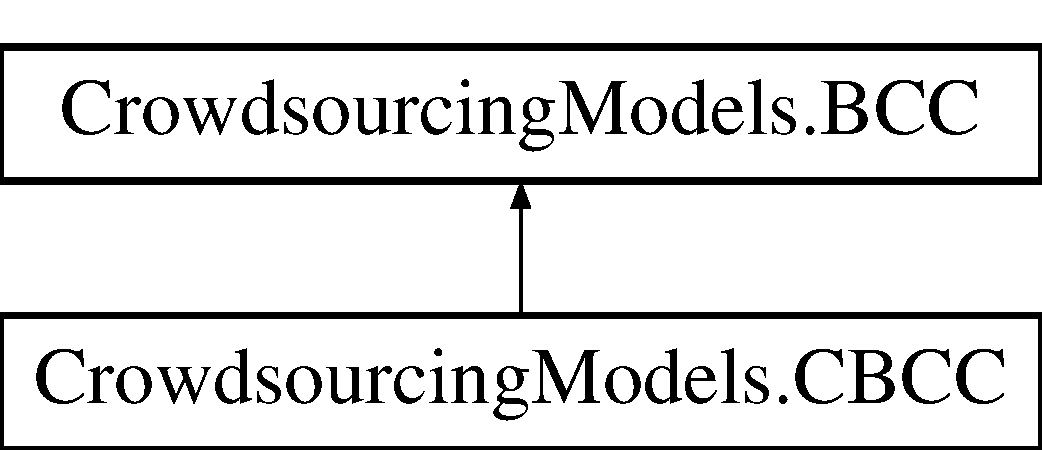
\includegraphics[height=2.000000cm]{class_crowdsourcing_models_1_1_b_c_c}
\end{center}
\end{figure}
\subsection*{Public Member Functions}
\begin{DoxyCompactItemize}
\item 
\hyperlink{class_crowdsourcing_models_1_1_b_c_c_aa8e876e451624f41cce4af6f38c3baf2}{B\+C\+C} ()
\begin{DoxyCompactList}\small\item\em Creates a \hyperlink{class_crowdsourcing_models_1_1_b_c_c}{B\+C\+C} model instance. \end{DoxyCompactList}\item 
virtual void \hyperlink{class_crowdsourcing_models_1_1_b_c_c_a7940c454f99a2b108723e8fcc49e035f}{Create\+Model} (int task\+Count, int label\+Count)
\begin{DoxyCompactList}\small\item\em Initializes the ranges, the generative process and the inference engine of the \hyperlink{class_crowdsourcing_models_1_1_b_c_c}{B\+C\+C} model. \end{DoxyCompactList}\item 
virtual \hyperlink{class_crowdsourcing_models_1_1_b_c_c_posteriors}{B\+C\+C\+Posteriors} \hyperlink{class_crowdsourcing_models_1_1_b_c_c_afa59a76d3c6fe11db2c3c037f8cf3efc}{Infer} (int\mbox{[}$\,$\mbox{]}\mbox{[}$\,$\mbox{]} task\+Indices, int\mbox{[}$\,$\mbox{]}\mbox{[}$\,$\mbox{]} worker\+Labels, \hyperlink{class_crowdsourcing_models_1_1_b_c_c_posteriors}{B\+C\+C\+Posteriors} priors)
\begin{DoxyCompactList}\small\item\em Infers the posteriors of \hyperlink{class_crowdsourcing_models_1_1_b_c_c}{B\+C\+C} using the attached data and priors. \end{DoxyCompactList}\item 
Dirichlet\mbox{[}$\,$\mbox{]} \hyperlink{class_crowdsourcing_models_1_1_b_c_c_aa31adcf5b6b498dd0bc86baa4f96434d}{Get\+Confusion\+Matrix\+Prior} ()
\begin{DoxyCompactList}\small\item\em Returns the confusion matrix prior of each worker. \end{DoxyCompactList}\end{DoxyCompactItemize}
\subsection*{Protected Member Functions}
\begin{DoxyCompactItemize}
\item 
virtual void \hyperlink{class_crowdsourcing_models_1_1_b_c_c_a3b4e301c3101dc790850548006d3aac8}{Define\+Variables\+And\+Ranges} (int task\+Count, int label\+Count)
\begin{DoxyCompactList}\small\item\em Initializes the ranges of the variables. \end{DoxyCompactList}\item 
virtual void \hyperlink{class_crowdsourcing_models_1_1_b_c_c_a0a4a80dc6093a006c87e43dcbf29c463}{Define\+Generative\+Process} ()
\begin{DoxyCompactList}\small\item\em Defines the \hyperlink{class_crowdsourcing_models_1_1_b_c_c}{B\+C\+C} generative process. \end{DoxyCompactList}\item 
virtual void \hyperlink{class_crowdsourcing_models_1_1_b_c_c_ab167badeccdb1951f97b6ed5b3b4dcd6}{Define\+Inference\+Engine} ()
\begin{DoxyCompactList}\small\item\em Initializes the \hyperlink{class_crowdsourcing_models_1_1_b_c_c}{B\+C\+C} inference engine. \end{DoxyCompactList}\item 
virtual void \hyperlink{class_crowdsourcing_models_1_1_b_c_c_ad08c9c0b6592cf6559118a68b56cfd07}{Set\+Priors} (int worker\+Count, \hyperlink{class_crowdsourcing_models_1_1_b_c_c_posteriors}{B\+C\+C\+Posteriors} priors)
\begin{DoxyCompactList}\small\item\em Sets the priors of \hyperlink{class_crowdsourcing_models_1_1_b_c_c}{B\+C\+C}. \end{DoxyCompactList}\item 
virtual void \hyperlink{class_crowdsourcing_models_1_1_b_c_c_af3806b7091a6bcc0116e3c8619d42daf}{Attach\+Data} (int\mbox{[}$\,$\mbox{]}\mbox{[}$\,$\mbox{]} task\+Indices, int\mbox{[}$\,$\mbox{]}\mbox{[}$\,$\mbox{]} worker\+Labels)
\begin{DoxyCompactList}\small\item\em Attachs the data to the workers labels. \end{DoxyCompactList}\item 
virtual void \hyperlink{class_crowdsourcing_models_1_1_b_c_c_ab40b3e7f5bd90c85672fb927a16f5fd6}{Attach\+Data} (int\mbox{[}$\,$\mbox{]}\mbox{[}$\,$\mbox{]} task\+Indices, int\mbox{[}$\,$\mbox{]}\mbox{[}$\,$\mbox{]} worker\+Labels, Dirichlet\mbox{[}$\,$\mbox{]}\mbox{[}$\,$\mbox{]} confusion\+Matrix\+Prior)
\begin{DoxyCompactList}\small\item\em Attachs the data to the workers labels with and sets the workers\textquotesingle{} confusion matrix priors. \end{DoxyCompactList}\end{DoxyCompactItemize}
\subsection*{Protected Attributes}
\begin{DoxyCompactItemize}
\item 
\hypertarget{class_crowdsourcing_models_1_1_b_c_c_aa58ee434d4e8d8b391040d117054938d}{}Range {\bfseries n}\label{class_crowdsourcing_models_1_1_b_c_c_aa58ee434d4e8d8b391040d117054938d}

\item 
\hypertarget{class_crowdsourcing_models_1_1_b_c_c_afd5435718898d47b9c3ff5594fa2f283}{}Range {\bfseries k}\label{class_crowdsourcing_models_1_1_b_c_c_afd5435718898d47b9c3ff5594fa2f283}

\item 
\hypertarget{class_crowdsourcing_models_1_1_b_c_c_a97200049317251fa92243337840b2328}{}Range {\bfseries c}\label{class_crowdsourcing_models_1_1_b_c_c_a97200049317251fa92243337840b2328}

\item 
\hypertarget{class_crowdsourcing_models_1_1_b_c_c_a2b3ffffefe49c01347455642fd863ef9}{}Range {\bfseries kn}\label{class_crowdsourcing_models_1_1_b_c_c_a2b3ffffefe49c01347455642fd863ef9}

\item 
\hypertarget{class_crowdsourcing_models_1_1_b_c_c_a685b9761476672147cc8936b1bfcc648}{}Variable$<$ int $>$ {\bfseries Worker\+Count}\label{class_crowdsourcing_models_1_1_b_c_c_a685b9761476672147cc8936b1bfcc648}

\item 
\hypertarget{class_crowdsourcing_models_1_1_b_c_c_a42f64f08ee33de60165c9e636f689434}{}Variable\+Array$<$ int $>$ {\bfseries True\+Label}\label{class_crowdsourcing_models_1_1_b_c_c_a42f64f08ee33de60165c9e636f689434}

\item 
\hypertarget{class_crowdsourcing_models_1_1_b_c_c_a0a39bdc086e5fbb275295379ba4d97a2}{}Variable\+Array$<$ int $>$ {\bfseries Worker\+Task\+Count}\label{class_crowdsourcing_models_1_1_b_c_c_a0a39bdc086e5fbb275295379ba4d97a2}

\item 
\hypertarget{class_crowdsourcing_models_1_1_b_c_c_a937ccca220ce098a54e11e19e57e6a40}{}Variable\+Array$<$ Variable\+Array$<$ int $>$, int\mbox{[}$\,$\mbox{]}\mbox{[}$\,$\mbox{]}$>$ {\bfseries Worker\+Task\+Index}\label{class_crowdsourcing_models_1_1_b_c_c_a937ccca220ce098a54e11e19e57e6a40}

\item 
\hypertarget{class_crowdsourcing_models_1_1_b_c_c_a725288eab6a1d504644e575538b8096f}{}Variable\+Array$<$ Variable\+Array$<$ int $>$, int\mbox{[}$\,$\mbox{]}\mbox{[}$\,$\mbox{]}$>$ {\bfseries Worker\+Label}\label{class_crowdsourcing_models_1_1_b_c_c_a725288eab6a1d504644e575538b8096f}

\item 
\hypertarget{class_crowdsourcing_models_1_1_b_c_c_aedd35546a335dd210693c23cdf33426b}{}Variable$<$ Vector $>$ {\bfseries Background\+Label\+Prob}\label{class_crowdsourcing_models_1_1_b_c_c_aedd35546a335dd210693c23cdf33426b}

\item 
\hypertarget{class_crowdsourcing_models_1_1_b_c_c_ac3423e1c181209e137446d9cfbed4a69}{}Variable\+Array$<$ Variable\+Array$<$ Vector $>$, Vector\mbox{[}$\,$\mbox{]}\mbox{[}$\,$\mbox{]}$>$ {\bfseries Worker\+Confusion\+Matrix}\label{class_crowdsourcing_models_1_1_b_c_c_ac3423e1c181209e137446d9cfbed4a69}

\item 
\hypertarget{class_crowdsourcing_models_1_1_b_c_c_a386f9905a19a7abaa35aec10517ad30f}{}Variable$<$ bool $>$ {\bfseries Evidence}\label{class_crowdsourcing_models_1_1_b_c_c_a386f9905a19a7abaa35aec10517ad30f}

\item 
\hypertarget{class_crowdsourcing_models_1_1_b_c_c_a3ef6845c2072f001f77835c1e891e958}{}Variable$<$ Dirichlet $>$ {\bfseries Background\+Label\+Prob\+Prior}\label{class_crowdsourcing_models_1_1_b_c_c_a3ef6845c2072f001f77835c1e891e958}

\item 
\hypertarget{class_crowdsourcing_models_1_1_b_c_c_a12a1e36fa58b81c5b06260b624dd315b}{}Variable\+Array$<$ Variable\+Array$<$ Dirichlet $>$, Dirichlet\mbox{[}$\,$\mbox{]}\mbox{[}$\,$\mbox{]}$>$ {\bfseries Confusion\+Matrix\+Prior}\label{class_crowdsourcing_models_1_1_b_c_c_a12a1e36fa58b81c5b06260b624dd315b}

\item 
\hypertarget{class_crowdsourcing_models_1_1_b_c_c_a3631ed583e4307a270b7b9b0c4f98d82}{}Variable\+Array$<$ Discrete $>$ {\bfseries True\+Label\+Constraint}\label{class_crowdsourcing_models_1_1_b_c_c_a3631ed583e4307a270b7b9b0c4f98d82}

\item 
\hypertarget{class_crowdsourcing_models_1_1_b_c_c_afc07115edd21cd40cc322e2bfcb0a5b3}{}Variable$<$ Bernoulli $>$ {\bfseries Evidence\+Prior}\label{class_crowdsourcing_models_1_1_b_c_c_afc07115edd21cd40cc322e2bfcb0a5b3}

\item 
\hypertarget{class_crowdsourcing_models_1_1_b_c_c_aafa91c4ced5cd1174a37b703cfc8b0b7}{}Inference\+Engine {\bfseries Engine}\label{class_crowdsourcing_models_1_1_b_c_c_aafa91c4ced5cd1174a37b703cfc8b0b7}

\end{DoxyCompactItemize}
\subsection*{Properties}
\begin{DoxyCompactItemize}
\item 
int \hyperlink{class_crowdsourcing_models_1_1_b_c_c_a38f7ecffc9acead6a585fab6ceae67a8}{Label\+Count}\hspace{0.3cm}{\ttfamily  \mbox{[}get\mbox{]}}
\begin{DoxyCompactList}\small\item\em The number of label values. \end{DoxyCompactList}\item 
int \hyperlink{class_crowdsourcing_models_1_1_b_c_c_a79d1a31d02990f09b9b88eff57ad1920}{Task\+Count}\hspace{0.3cm}{\ttfamily  \mbox{[}get\mbox{]}}
\begin{DoxyCompactList}\small\item\em The number of tasks. \end{DoxyCompactList}\item 
\hypertarget{class_crowdsourcing_models_1_1_b_c_c_abb3255af092632ce5366f536b73f8d7e}{}double {\bfseries Initial\+Worker\+Belief}\hspace{0.3cm}{\ttfamily  \mbox{[}get, set\mbox{]}}\label{class_crowdsourcing_models_1_1_b_c_c_abb3255af092632ce5366f536b73f8d7e}

\item 
int \hyperlink{class_crowdsourcing_models_1_1_b_c_c_aa5cce09f39a4144782ac97f490747792}{Number\+Of\+Iterations}\hspace{0.3cm}{\ttfamily  \mbox{[}get, set\mbox{]}}
\begin{DoxyCompactList}\small\item\em The number of inference iterations. \end{DoxyCompactList}\end{DoxyCompactItemize}


\subsection{Detailed Description}
The \hyperlink{class_crowdsourcing_models_1_1_b_c_c}{B\+C\+C} model class. 



\subsection{Constructor \& Destructor Documentation}
\hypertarget{class_crowdsourcing_models_1_1_b_c_c_aa8e876e451624f41cce4af6f38c3baf2}{}\index{Crowdsourcing\+Models\+::\+B\+C\+C@{Crowdsourcing\+Models\+::\+B\+C\+C}!B\+C\+C@{B\+C\+C}}
\index{B\+C\+C@{B\+C\+C}!Crowdsourcing\+Models\+::\+B\+C\+C@{Crowdsourcing\+Models\+::\+B\+C\+C}}
\subsubsection[{B\+C\+C()}]{\setlength{\rightskip}{0pt plus 5cm}Crowdsourcing\+Models.\+B\+C\+C.\+B\+C\+C (
\begin{DoxyParamCaption}
{}
\end{DoxyParamCaption}
)\hspace{0.3cm}{\ttfamily [inline]}}\label{class_crowdsourcing_models_1_1_b_c_c_aa8e876e451624f41cce4af6f38c3baf2}


Creates a \hyperlink{class_crowdsourcing_models_1_1_b_c_c}{B\+C\+C} model instance. 



\subsection{Member Function Documentation}
\hypertarget{class_crowdsourcing_models_1_1_b_c_c_af3806b7091a6bcc0116e3c8619d42daf}{}\index{Crowdsourcing\+Models\+::\+B\+C\+C@{Crowdsourcing\+Models\+::\+B\+C\+C}!Attach\+Data@{Attach\+Data}}
\index{Attach\+Data@{Attach\+Data}!Crowdsourcing\+Models\+::\+B\+C\+C@{Crowdsourcing\+Models\+::\+B\+C\+C}}
\subsubsection[{Attach\+Data(int[][] task\+Indices, int[][] worker\+Labels)}]{\setlength{\rightskip}{0pt plus 5cm}virtual void Crowdsourcing\+Models.\+B\+C\+C.\+Attach\+Data (
\begin{DoxyParamCaption}
\item[{int}]{task\+Indices\mbox{[}$\,$\mbox{]}\mbox{[}$\,$\mbox{]}, }
\item[{int}]{worker\+Labels\mbox{[}$\,$\mbox{]}\mbox{[}$\,$\mbox{]}}
\end{DoxyParamCaption}
)\hspace{0.3cm}{\ttfamily [inline]}, {\ttfamily [protected]}, {\ttfamily [virtual]}}\label{class_crowdsourcing_models_1_1_b_c_c_af3806b7091a6bcc0116e3c8619d42daf}


Attachs the data to the workers labels. 


\begin{DoxyParams}{Parameters}
{\em task\+Indices} & The matrix of the task indices (columns) of each worker (rows).\\
\hline
{\em worker\+Labels} & The matrix of the labels (columns) of each worker (rows).\\
\hline
\end{DoxyParams}


Reimplemented in \hyperlink{class_crowdsourcing_models_1_1_c_b_c_c_a768dbc90e6215dafc03e3bab5df4eb5c}{Crowdsourcing\+Models.\+C\+B\+C\+C}.

\hypertarget{class_crowdsourcing_models_1_1_b_c_c_ab40b3e7f5bd90c85672fb927a16f5fd6}{}\index{Crowdsourcing\+Models\+::\+B\+C\+C@{Crowdsourcing\+Models\+::\+B\+C\+C}!Attach\+Data@{Attach\+Data}}
\index{Attach\+Data@{Attach\+Data}!Crowdsourcing\+Models\+::\+B\+C\+C@{Crowdsourcing\+Models\+::\+B\+C\+C}}
\subsubsection[{Attach\+Data(int[][] task\+Indices, int[][] worker\+Labels, Dirichlet[][] confusion\+Matrix\+Prior)}]{\setlength{\rightskip}{0pt plus 5cm}virtual void Crowdsourcing\+Models.\+B\+C\+C.\+Attach\+Data (
\begin{DoxyParamCaption}
\item[{int}]{task\+Indices\mbox{[}$\,$\mbox{]}\mbox{[}$\,$\mbox{]}, }
\item[{int}]{worker\+Labels\mbox{[}$\,$\mbox{]}\mbox{[}$\,$\mbox{]}, }
\item[{Dirichlet}]{confusion\+Matrix\+Prior\mbox{[}$\,$\mbox{]}\mbox{[}$\,$\mbox{]}}
\end{DoxyParamCaption}
)\hspace{0.3cm}{\ttfamily [inline]}, {\ttfamily [protected]}, {\ttfamily [virtual]}}\label{class_crowdsourcing_models_1_1_b_c_c_ab40b3e7f5bd90c85672fb927a16f5fd6}


Attachs the data to the workers labels with and sets the workers\textquotesingle{} confusion matrix priors. 


\begin{DoxyParams}{Parameters}
{\em task\+Indices} & The matrix of the task indices (columns) of each worker (rows).\\
\hline
{\em worker\+Labels} & The matrix of the labels (columns) of each worker (rows).\\
\hline
{\em confusion\+Matrix\+Prior} & The workers\textquotesingle{} confusion matrix priors.\\
\hline
\end{DoxyParams}
\hypertarget{class_crowdsourcing_models_1_1_b_c_c_a7940c454f99a2b108723e8fcc49e035f}{}\index{Crowdsourcing\+Models\+::\+B\+C\+C@{Crowdsourcing\+Models\+::\+B\+C\+C}!Create\+Model@{Create\+Model}}
\index{Create\+Model@{Create\+Model}!Crowdsourcing\+Models\+::\+B\+C\+C@{Crowdsourcing\+Models\+::\+B\+C\+C}}
\subsubsection[{Create\+Model(int task\+Count, int label\+Count)}]{\setlength{\rightskip}{0pt plus 5cm}virtual void Crowdsourcing\+Models.\+B\+C\+C.\+Create\+Model (
\begin{DoxyParamCaption}
\item[{int}]{task\+Count, }
\item[{int}]{label\+Count}
\end{DoxyParamCaption}
)\hspace{0.3cm}{\ttfamily [inline]}, {\ttfamily [virtual]}}\label{class_crowdsourcing_models_1_1_b_c_c_a7940c454f99a2b108723e8fcc49e035f}


Initializes the ranges, the generative process and the inference engine of the \hyperlink{class_crowdsourcing_models_1_1_b_c_c}{B\+C\+C} model. 


\begin{DoxyParams}{Parameters}
{\em task\+Count} & The number of tasks.\\
\hline
{\em label\+Count} & The number of labels.\\
\hline
\end{DoxyParams}


Reimplemented in \hyperlink{class_crowdsourcing_models_1_1_c_b_c_c_a9dc55362a1a756ced24bb3736075a180}{Crowdsourcing\+Models.\+C\+B\+C\+C}.

\hypertarget{class_crowdsourcing_models_1_1_b_c_c_a0a4a80dc6093a006c87e43dcbf29c463}{}\index{Crowdsourcing\+Models\+::\+B\+C\+C@{Crowdsourcing\+Models\+::\+B\+C\+C}!Define\+Generative\+Process@{Define\+Generative\+Process}}
\index{Define\+Generative\+Process@{Define\+Generative\+Process}!Crowdsourcing\+Models\+::\+B\+C\+C@{Crowdsourcing\+Models\+::\+B\+C\+C}}
\subsubsection[{Define\+Generative\+Process()}]{\setlength{\rightskip}{0pt plus 5cm}virtual void Crowdsourcing\+Models.\+B\+C\+C.\+Define\+Generative\+Process (
\begin{DoxyParamCaption}
{}
\end{DoxyParamCaption}
)\hspace{0.3cm}{\ttfamily [inline]}, {\ttfamily [protected]}, {\ttfamily [virtual]}}\label{class_crowdsourcing_models_1_1_b_c_c_a0a4a80dc6093a006c87e43dcbf29c463}


Defines the \hyperlink{class_crowdsourcing_models_1_1_b_c_c}{B\+C\+C} generative process. 



Reimplemented in \hyperlink{class_crowdsourcing_models_1_1_c_b_c_c_a11449d19d584834a5de6c877763d829e}{Crowdsourcing\+Models.\+C\+B\+C\+C}.

\hypertarget{class_crowdsourcing_models_1_1_b_c_c_ab167badeccdb1951f97b6ed5b3b4dcd6}{}\index{Crowdsourcing\+Models\+::\+B\+C\+C@{Crowdsourcing\+Models\+::\+B\+C\+C}!Define\+Inference\+Engine@{Define\+Inference\+Engine}}
\index{Define\+Inference\+Engine@{Define\+Inference\+Engine}!Crowdsourcing\+Models\+::\+B\+C\+C@{Crowdsourcing\+Models\+::\+B\+C\+C}}
\subsubsection[{Define\+Inference\+Engine()}]{\setlength{\rightskip}{0pt plus 5cm}virtual void Crowdsourcing\+Models.\+B\+C\+C.\+Define\+Inference\+Engine (
\begin{DoxyParamCaption}
{}
\end{DoxyParamCaption}
)\hspace{0.3cm}{\ttfamily [inline]}, {\ttfamily [protected]}, {\ttfamily [virtual]}}\label{class_crowdsourcing_models_1_1_b_c_c_ab167badeccdb1951f97b6ed5b3b4dcd6}


Initializes the \hyperlink{class_crowdsourcing_models_1_1_b_c_c}{B\+C\+C} inference engine. 



Reimplemented in \hyperlink{class_crowdsourcing_models_1_1_c_b_c_c_a48270c4aca4a4d42f0a914772950ac9d}{Crowdsourcing\+Models.\+C\+B\+C\+C}.

\hypertarget{class_crowdsourcing_models_1_1_b_c_c_a3b4e301c3101dc790850548006d3aac8}{}\index{Crowdsourcing\+Models\+::\+B\+C\+C@{Crowdsourcing\+Models\+::\+B\+C\+C}!Define\+Variables\+And\+Ranges@{Define\+Variables\+And\+Ranges}}
\index{Define\+Variables\+And\+Ranges@{Define\+Variables\+And\+Ranges}!Crowdsourcing\+Models\+::\+B\+C\+C@{Crowdsourcing\+Models\+::\+B\+C\+C}}
\subsubsection[{Define\+Variables\+And\+Ranges(int task\+Count, int label\+Count)}]{\setlength{\rightskip}{0pt plus 5cm}virtual void Crowdsourcing\+Models.\+B\+C\+C.\+Define\+Variables\+And\+Ranges (
\begin{DoxyParamCaption}
\item[{int}]{task\+Count, }
\item[{int}]{label\+Count}
\end{DoxyParamCaption}
)\hspace{0.3cm}{\ttfamily [inline]}, {\ttfamily [protected]}, {\ttfamily [virtual]}}\label{class_crowdsourcing_models_1_1_b_c_c_a3b4e301c3101dc790850548006d3aac8}


Initializes the ranges of the variables. 


\begin{DoxyParams}{Parameters}
{\em task\+Count} & The number of tasks.\\
\hline
{\em label\+Count} & The number of labels.\\
\hline
\end{DoxyParams}


Reimplemented in \hyperlink{class_crowdsourcing_models_1_1_c_b_c_c_a33085b5a8b123a62a890eca1367a40ba}{Crowdsourcing\+Models.\+C\+B\+C\+C}.

\hypertarget{class_crowdsourcing_models_1_1_b_c_c_aa31adcf5b6b498dd0bc86baa4f96434d}{}\index{Crowdsourcing\+Models\+::\+B\+C\+C@{Crowdsourcing\+Models\+::\+B\+C\+C}!Get\+Confusion\+Matrix\+Prior@{Get\+Confusion\+Matrix\+Prior}}
\index{Get\+Confusion\+Matrix\+Prior@{Get\+Confusion\+Matrix\+Prior}!Crowdsourcing\+Models\+::\+B\+C\+C@{Crowdsourcing\+Models\+::\+B\+C\+C}}
\subsubsection[{Get\+Confusion\+Matrix\+Prior()}]{\setlength{\rightskip}{0pt plus 5cm}Dirichlet \mbox{[}$\,$\mbox{]} Crowdsourcing\+Models.\+B\+C\+C.\+Get\+Confusion\+Matrix\+Prior (
\begin{DoxyParamCaption}
{}
\end{DoxyParamCaption}
)\hspace{0.3cm}{\ttfamily [inline]}}\label{class_crowdsourcing_models_1_1_b_c_c_aa31adcf5b6b498dd0bc86baa4f96434d}


Returns the confusion matrix prior of each worker. 

\begin{DoxyReturn}{Returns}
The confusion matrix prior of each worker.
\end{DoxyReturn}
\hypertarget{class_crowdsourcing_models_1_1_b_c_c_afa59a76d3c6fe11db2c3c037f8cf3efc}{}\index{Crowdsourcing\+Models\+::\+B\+C\+C@{Crowdsourcing\+Models\+::\+B\+C\+C}!Infer@{Infer}}
\index{Infer@{Infer}!Crowdsourcing\+Models\+::\+B\+C\+C@{Crowdsourcing\+Models\+::\+B\+C\+C}}
\subsubsection[{Infer(int[][] task\+Indices, int[][] worker\+Labels, B\+C\+C\+Posteriors priors)}]{\setlength{\rightskip}{0pt plus 5cm}virtual {\bf B\+C\+C\+Posteriors} Crowdsourcing\+Models.\+B\+C\+C.\+Infer (
\begin{DoxyParamCaption}
\item[{int}]{task\+Indices\mbox{[}$\,$\mbox{]}\mbox{[}$\,$\mbox{]}, }
\item[{int}]{worker\+Labels\mbox{[}$\,$\mbox{]}\mbox{[}$\,$\mbox{]}, }
\item[{{\bf B\+C\+C\+Posteriors}}]{priors}
\end{DoxyParamCaption}
)\hspace{0.3cm}{\ttfamily [inline]}, {\ttfamily [virtual]}}\label{class_crowdsourcing_models_1_1_b_c_c_afa59a76d3c6fe11db2c3c037f8cf3efc}


Infers the posteriors of \hyperlink{class_crowdsourcing_models_1_1_b_c_c}{B\+C\+C} using the attached data and priors. 


\begin{DoxyParams}{Parameters}
{\em task\+Indices} & The matrix of the task indices (columns) of each worker (rows).\\
\hline
{\em worker\+Labels} & The matrix of the labels (columns) of each worker (rows).\\
\hline
{\em priors} & The priors of the \hyperlink{class_crowdsourcing_models_1_1_b_c_c}{B\+C\+C} parameters.\\
\hline
\end{DoxyParams}
\begin{DoxyReturn}{Returns}

\end{DoxyReturn}


Reimplemented in \hyperlink{class_crowdsourcing_models_1_1_c_b_c_c_a538743585401f436f10bfc46c26c767a}{Crowdsourcing\+Models.\+C\+B\+C\+C}.

\hypertarget{class_crowdsourcing_models_1_1_b_c_c_ad08c9c0b6592cf6559118a68b56cfd07}{}\index{Crowdsourcing\+Models\+::\+B\+C\+C@{Crowdsourcing\+Models\+::\+B\+C\+C}!Set\+Priors@{Set\+Priors}}
\index{Set\+Priors@{Set\+Priors}!Crowdsourcing\+Models\+::\+B\+C\+C@{Crowdsourcing\+Models\+::\+B\+C\+C}}
\subsubsection[{Set\+Priors(int worker\+Count, B\+C\+C\+Posteriors priors)}]{\setlength{\rightskip}{0pt plus 5cm}virtual void Crowdsourcing\+Models.\+B\+C\+C.\+Set\+Priors (
\begin{DoxyParamCaption}
\item[{int}]{worker\+Count, }
\item[{{\bf B\+C\+C\+Posteriors}}]{priors}
\end{DoxyParamCaption}
)\hspace{0.3cm}{\ttfamily [inline]}, {\ttfamily [protected]}, {\ttfamily [virtual]}}\label{class_crowdsourcing_models_1_1_b_c_c_ad08c9c0b6592cf6559118a68b56cfd07}


Sets the priors of \hyperlink{class_crowdsourcing_models_1_1_b_c_c}{B\+C\+C}. 


\begin{DoxyParams}{Parameters}
{\em worker\+Count} & The number of workers.\\
\hline
{\em priors} & The priors.\\
\hline
\end{DoxyParams}


Reimplemented in \hyperlink{class_crowdsourcing_models_1_1_c_b_c_c_ab662d32f67474b73ad0ca6915d59901d}{Crowdsourcing\+Models.\+C\+B\+C\+C}.



\subsection{Property Documentation}
\hypertarget{class_crowdsourcing_models_1_1_b_c_c_a38f7ecffc9acead6a585fab6ceae67a8}{}\index{Crowdsourcing\+Models\+::\+B\+C\+C@{Crowdsourcing\+Models\+::\+B\+C\+C}!Label\+Count@{Label\+Count}}
\index{Label\+Count@{Label\+Count}!Crowdsourcing\+Models\+::\+B\+C\+C@{Crowdsourcing\+Models\+::\+B\+C\+C}}
\subsubsection[{Label\+Count}]{\setlength{\rightskip}{0pt plus 5cm}int Crowdsourcing\+Models.\+B\+C\+C.\+Label\+Count\hspace{0.3cm}{\ttfamily [get]}}\label{class_crowdsourcing_models_1_1_b_c_c_a38f7ecffc9acead6a585fab6ceae67a8}


The number of label values. 

\hypertarget{class_crowdsourcing_models_1_1_b_c_c_aa5cce09f39a4144782ac97f490747792}{}\index{Crowdsourcing\+Models\+::\+B\+C\+C@{Crowdsourcing\+Models\+::\+B\+C\+C}!Number\+Of\+Iterations@{Number\+Of\+Iterations}}
\index{Number\+Of\+Iterations@{Number\+Of\+Iterations}!Crowdsourcing\+Models\+::\+B\+C\+C@{Crowdsourcing\+Models\+::\+B\+C\+C}}
\subsubsection[{Number\+Of\+Iterations}]{\setlength{\rightskip}{0pt plus 5cm}int Crowdsourcing\+Models.\+B\+C\+C.\+Number\+Of\+Iterations\hspace{0.3cm}{\ttfamily [get]}, {\ttfamily [set]}}\label{class_crowdsourcing_models_1_1_b_c_c_aa5cce09f39a4144782ac97f490747792}


The number of inference iterations. 

\hypertarget{class_crowdsourcing_models_1_1_b_c_c_a79d1a31d02990f09b9b88eff57ad1920}{}\index{Crowdsourcing\+Models\+::\+B\+C\+C@{Crowdsourcing\+Models\+::\+B\+C\+C}!Task\+Count@{Task\+Count}}
\index{Task\+Count@{Task\+Count}!Crowdsourcing\+Models\+::\+B\+C\+C@{Crowdsourcing\+Models\+::\+B\+C\+C}}
\subsubsection[{Task\+Count}]{\setlength{\rightskip}{0pt plus 5cm}int Crowdsourcing\+Models.\+B\+C\+C.\+Task\+Count\hspace{0.3cm}{\ttfamily [get]}}\label{class_crowdsourcing_models_1_1_b_c_c_a79d1a31d02990f09b9b88eff57ad1920}


The number of tasks. 



The documentation for this class was generated from the following file\+:\begin{DoxyCompactItemize}
\item 
C\+:/\+Users/\+Matteo/\+Source/\+Repos/active-\/crowd/\+Crowdsourcing\+Models/B\+C\+C.\+cs\end{DoxyCompactItemize}

\hypertarget{class_crowdsourcing_models_1_1_b_c_c_posteriors}{}\section{Crowdsourcing\+Models.\+B\+C\+C\+Posteriors Class Reference}
\label{class_crowdsourcing_models_1_1_b_c_c_posteriors}\index{Crowdsourcing\+Models.\+B\+C\+C\+Posteriors@{Crowdsourcing\+Models.\+B\+C\+C\+Posteriors}}


The \hyperlink{class_crowdsourcing_models_1_1_b_c_c}{B\+C\+C} posteriors class.  


Inheritance diagram for Crowdsourcing\+Models.\+B\+C\+C\+Posteriors\+:\begin{figure}[H]
\begin{center}
\leavevmode
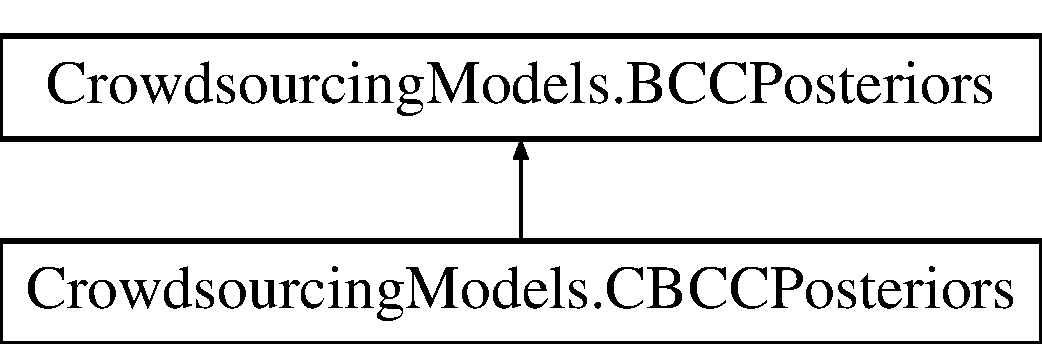
\includegraphics[height=2.000000cm]{class_crowdsourcing_models_1_1_b_c_c_posteriors}
\end{center}
\end{figure}
\subsection*{Public Attributes}
\begin{DoxyCompactItemize}
\item 
Dirichlet \hyperlink{class_crowdsourcing_models_1_1_b_c_c_posteriors_aaac52193d90fcc91d50472ddf6683eab}{Background\+Label\+Prob}
\begin{DoxyCompactList}\small\item\em The probabilities that generate the true labels of all the tasks. \end{DoxyCompactList}\item 
Discrete\mbox{[}$\,$\mbox{]} \hyperlink{class_crowdsourcing_models_1_1_b_c_c_posteriors_ab5020db40be02d3dedd50d61371e84c8}{True\+Label}
\begin{DoxyCompactList}\small\item\em The probabilities of the true label of each task. \end{DoxyCompactList}\item 
Dirichlet\mbox{[}$\,$\mbox{]}\mbox{[}$\,$\mbox{]} \hyperlink{class_crowdsourcing_models_1_1_b_c_c_posteriors_ab9ba40964b3fa2c9c349282dafa79fbb}{Worker\+Confusion\+Matrix}
\begin{DoxyCompactList}\small\item\em The Dirichlet parameters of the confusion matrix of each worker. \end{DoxyCompactList}\item 
Discrete\mbox{[}$\,$\mbox{]}\mbox{[}$\,$\mbox{]} \hyperlink{class_crowdsourcing_models_1_1_b_c_c_posteriors_a2bf09db28d0e9cdf9c6816c9e798ec95}{Worker\+Prediction}
\begin{DoxyCompactList}\small\item\em The predictive probabilities of the worker\textquotesingle{}s labels. \end{DoxyCompactList}\item 
Discrete\mbox{[}$\,$\mbox{]} \hyperlink{class_crowdsourcing_models_1_1_b_c_c_posteriors_ac3b5fc60bf5d2a625a7638bf5af91474}{True\+Label\+Constraint}
\begin{DoxyCompactList}\small\item\em The true label constraint used in online training. \end{DoxyCompactList}\item 
Bernoulli \hyperlink{class_crowdsourcing_models_1_1_b_c_c_posteriors_a9b35421059e1ce53b9eadccfe4d559bf}{Evidence}
\begin{DoxyCompactList}\small\item\em The model evidence. \end{DoxyCompactList}\end{DoxyCompactItemize}


\subsection{Detailed Description}
The \hyperlink{class_crowdsourcing_models_1_1_b_c_c}{B\+C\+C} posteriors class. 



\subsection{Member Data Documentation}
\hypertarget{class_crowdsourcing_models_1_1_b_c_c_posteriors_aaac52193d90fcc91d50472ddf6683eab}{}\index{Crowdsourcing\+Models\+::\+B\+C\+C\+Posteriors@{Crowdsourcing\+Models\+::\+B\+C\+C\+Posteriors}!Background\+Label\+Prob@{Background\+Label\+Prob}}
\index{Background\+Label\+Prob@{Background\+Label\+Prob}!Crowdsourcing\+Models\+::\+B\+C\+C\+Posteriors@{Crowdsourcing\+Models\+::\+B\+C\+C\+Posteriors}}
\subsubsection[{Background\+Label\+Prob}]{\setlength{\rightskip}{0pt plus 5cm}Dirichlet Crowdsourcing\+Models.\+B\+C\+C\+Posteriors.\+Background\+Label\+Prob}\label{class_crowdsourcing_models_1_1_b_c_c_posteriors_aaac52193d90fcc91d50472ddf6683eab}


The probabilities that generate the true labels of all the tasks. 

\hypertarget{class_crowdsourcing_models_1_1_b_c_c_posteriors_a9b35421059e1ce53b9eadccfe4d559bf}{}\index{Crowdsourcing\+Models\+::\+B\+C\+C\+Posteriors@{Crowdsourcing\+Models\+::\+B\+C\+C\+Posteriors}!Evidence@{Evidence}}
\index{Evidence@{Evidence}!Crowdsourcing\+Models\+::\+B\+C\+C\+Posteriors@{Crowdsourcing\+Models\+::\+B\+C\+C\+Posteriors}}
\subsubsection[{Evidence}]{\setlength{\rightskip}{0pt plus 5cm}Bernoulli Crowdsourcing\+Models.\+B\+C\+C\+Posteriors.\+Evidence}\label{class_crowdsourcing_models_1_1_b_c_c_posteriors_a9b35421059e1ce53b9eadccfe4d559bf}


The model evidence. 

\hypertarget{class_crowdsourcing_models_1_1_b_c_c_posteriors_ab5020db40be02d3dedd50d61371e84c8}{}\index{Crowdsourcing\+Models\+::\+B\+C\+C\+Posteriors@{Crowdsourcing\+Models\+::\+B\+C\+C\+Posteriors}!True\+Label@{True\+Label}}
\index{True\+Label@{True\+Label}!Crowdsourcing\+Models\+::\+B\+C\+C\+Posteriors@{Crowdsourcing\+Models\+::\+B\+C\+C\+Posteriors}}
\subsubsection[{True\+Label}]{\setlength{\rightskip}{0pt plus 5cm}Discrete \mbox{[}$\,$\mbox{]} Crowdsourcing\+Models.\+B\+C\+C\+Posteriors.\+True\+Label}\label{class_crowdsourcing_models_1_1_b_c_c_posteriors_ab5020db40be02d3dedd50d61371e84c8}


The probabilities of the true label of each task. 

\hypertarget{class_crowdsourcing_models_1_1_b_c_c_posteriors_ac3b5fc60bf5d2a625a7638bf5af91474}{}\index{Crowdsourcing\+Models\+::\+B\+C\+C\+Posteriors@{Crowdsourcing\+Models\+::\+B\+C\+C\+Posteriors}!True\+Label\+Constraint@{True\+Label\+Constraint}}
\index{True\+Label\+Constraint@{True\+Label\+Constraint}!Crowdsourcing\+Models\+::\+B\+C\+C\+Posteriors@{Crowdsourcing\+Models\+::\+B\+C\+C\+Posteriors}}
\subsubsection[{True\+Label\+Constraint}]{\setlength{\rightskip}{0pt plus 5cm}Discrete \mbox{[}$\,$\mbox{]} Crowdsourcing\+Models.\+B\+C\+C\+Posteriors.\+True\+Label\+Constraint}\label{class_crowdsourcing_models_1_1_b_c_c_posteriors_ac3b5fc60bf5d2a625a7638bf5af91474}


The true label constraint used in online training. 

\hypertarget{class_crowdsourcing_models_1_1_b_c_c_posteriors_ab9ba40964b3fa2c9c349282dafa79fbb}{}\index{Crowdsourcing\+Models\+::\+B\+C\+C\+Posteriors@{Crowdsourcing\+Models\+::\+B\+C\+C\+Posteriors}!Worker\+Confusion\+Matrix@{Worker\+Confusion\+Matrix}}
\index{Worker\+Confusion\+Matrix@{Worker\+Confusion\+Matrix}!Crowdsourcing\+Models\+::\+B\+C\+C\+Posteriors@{Crowdsourcing\+Models\+::\+B\+C\+C\+Posteriors}}
\subsubsection[{Worker\+Confusion\+Matrix}]{\setlength{\rightskip}{0pt plus 5cm}Dirichlet \mbox{[}$\,$\mbox{]}\mbox{[}$\,$\mbox{]} Crowdsourcing\+Models.\+B\+C\+C\+Posteriors.\+Worker\+Confusion\+Matrix}\label{class_crowdsourcing_models_1_1_b_c_c_posteriors_ab9ba40964b3fa2c9c349282dafa79fbb}


The Dirichlet parameters of the confusion matrix of each worker. 

\hypertarget{class_crowdsourcing_models_1_1_b_c_c_posteriors_a2bf09db28d0e9cdf9c6816c9e798ec95}{}\index{Crowdsourcing\+Models\+::\+B\+C\+C\+Posteriors@{Crowdsourcing\+Models\+::\+B\+C\+C\+Posteriors}!Worker\+Prediction@{Worker\+Prediction}}
\index{Worker\+Prediction@{Worker\+Prediction}!Crowdsourcing\+Models\+::\+B\+C\+C\+Posteriors@{Crowdsourcing\+Models\+::\+B\+C\+C\+Posteriors}}
\subsubsection[{Worker\+Prediction}]{\setlength{\rightskip}{0pt plus 5cm}Discrete \mbox{[}$\,$\mbox{]}\mbox{[}$\,$\mbox{]} Crowdsourcing\+Models.\+B\+C\+C\+Posteriors.\+Worker\+Prediction}\label{class_crowdsourcing_models_1_1_b_c_c_posteriors_a2bf09db28d0e9cdf9c6816c9e798ec95}


The predictive probabilities of the worker\textquotesingle{}s labels. 



The documentation for this class was generated from the following file\+:\begin{DoxyCompactItemize}
\item 
C\+:/\+Users/\+Matteo/\+Source/\+Repos/active-\/crowd/\+Crowdsourcing\+Models/B\+C\+C.\+cs\end{DoxyCompactItemize}

\hypertarget{class_crowdsourcing_models_1_1_c_b_c_c}{}\section{Crowdsourcing\+Models.\+C\+B\+C\+C Class Reference}
\label{class_crowdsourcing_models_1_1_c_b_c_c}\index{Crowdsourcing\+Models.\+C\+B\+C\+C@{Crowdsourcing\+Models.\+C\+B\+C\+C}}


The \hyperlink{class_crowdsourcing_models_1_1_c_b_c_c}{C\+B\+C\+C} model class.  


Inheritance diagram for Crowdsourcing\+Models.\+C\+B\+C\+C\+:\begin{figure}[H]
\begin{center}
\leavevmode
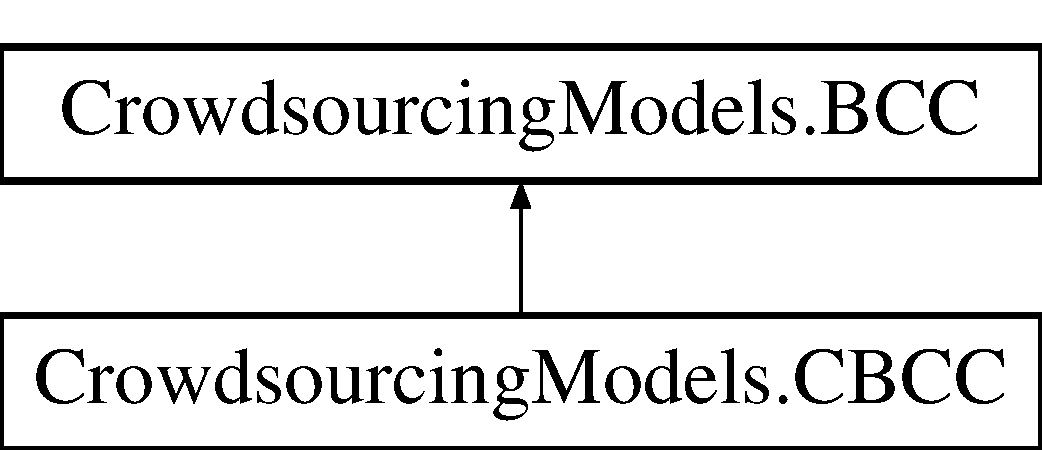
\includegraphics[height=2.000000cm]{class_crowdsourcing_models_1_1_c_b_c_c}
\end{center}
\end{figure}
\subsection*{Public Member Functions}
\begin{DoxyCompactItemize}
\item 
\hypertarget{class_crowdsourcing_models_1_1_c_b_c_c_a05bfcace3952fc2c97faad29b01cc5c2}{}void {\bfseries Set\+Community\+Count} (int \hyperlink{class_crowdsourcing_models_1_1_c_b_c_c_ab5f136f59f47bf4c8b35c36b227ab88c}{Community\+Count})\label{class_crowdsourcing_models_1_1_c_b_c_c_a05bfcace3952fc2c97faad29b01cc5c2}

\item 
\hyperlink{class_crowdsourcing_models_1_1_c_b_c_c_af72e2fcbacf20df12023895de3639301}{C\+B\+C\+C} ()
\begin{DoxyCompactList}\small\item\em Creates a \hyperlink{class_crowdsourcing_models_1_1_c_b_c_c}{C\+B\+C\+C} model instance. \end{DoxyCompactList}\item 
override void \hyperlink{class_crowdsourcing_models_1_1_c_b_c_c_a9dc55362a1a756ced24bb3736075a180}{Create\+Model} (int task\+Count, int label\+Count)
\begin{DoxyCompactList}\small\item\em Initializes the \hyperlink{class_crowdsourcing_models_1_1_c_b_c_c}{C\+B\+C\+C} model. \end{DoxyCompactList}\item 
virtual void \hyperlink{class_crowdsourcing_models_1_1_c_b_c_c_aeea050e9262f77d369278506586ef862}{Create\+Model} (int task\+Count, int label\+Count, int community\+Count)
\begin{DoxyCompactList}\small\item\em Initializes the \hyperlink{class_crowdsourcing_models_1_1_c_b_c_c}{C\+B\+C\+C} model with a number of communities. \end{DoxyCompactList}\item 
override \hyperlink{class_crowdsourcing_models_1_1_b_c_c_posteriors}{B\+C\+C\+Posteriors} \hyperlink{class_crowdsourcing_models_1_1_c_b_c_c_a538743585401f436f10bfc46c26c767a}{Infer} (int\mbox{[}$\,$\mbox{]}\mbox{[}$\,$\mbox{]} task\+Indices, int\mbox{[}$\,$\mbox{]}\mbox{[}$\,$\mbox{]} worker\+Labels, \hyperlink{class_crowdsourcing_models_1_1_b_c_c_posteriors}{B\+C\+C\+Posteriors} priors)
\begin{DoxyCompactList}\small\item\em Infers the posteriors of \hyperlink{class_crowdsourcing_models_1_1_c_b_c_c}{C\+B\+C\+C} using the attached data. \end{DoxyCompactList}\end{DoxyCompactItemize}
\subsection*{Protected Member Functions}
\begin{DoxyCompactItemize}
\item 
override void \hyperlink{class_crowdsourcing_models_1_1_c_b_c_c_a33085b5a8b123a62a890eca1367a40ba}{Define\+Variables\+And\+Ranges} (int task\+Count, int label\+Count)
\begin{DoxyCompactList}\small\item\em Defines the variables and the ranges of \hyperlink{class_crowdsourcing_models_1_1_c_b_c_c}{C\+B\+C\+C}. \end{DoxyCompactList}\item 
override void \hyperlink{class_crowdsourcing_models_1_1_c_b_c_c_a11449d19d584834a5de6c877763d829e}{Define\+Generative\+Process} ()
\begin{DoxyCompactList}\small\item\em Defines the generative process of \hyperlink{class_crowdsourcing_models_1_1_c_b_c_c}{C\+B\+C\+C}. \end{DoxyCompactList}\item 
override void \hyperlink{class_crowdsourcing_models_1_1_c_b_c_c_a48270c4aca4a4d42f0a914772950ac9d}{Define\+Inference\+Engine} ()
\begin{DoxyCompactList}\small\item\em Initializes the \hyperlink{class_crowdsourcing_models_1_1_c_b_c_c}{C\+B\+C\+C} inference engine. \end{DoxyCompactList}\item 
override void \hyperlink{class_crowdsourcing_models_1_1_c_b_c_c_a768dbc90e6215dafc03e3bab5df4eb5c}{Attach\+Data} (int\mbox{[}$\,$\mbox{]}\mbox{[}$\,$\mbox{]} task\+Indices, int\mbox{[}$\,$\mbox{]}\mbox{[}$\,$\mbox{]} worker\+Labels)
\begin{DoxyCompactList}\small\item\em Attachs the data to the workers labels. \end{DoxyCompactList}\item 
void \hyperlink{class_crowdsourcing_models_1_1_c_b_c_c_a466df8df2843675faf22a20531a8e54d}{Attach\+Data} (int\mbox{[}$\,$\mbox{]}\mbox{[}$\,$\mbox{]} task\+Indices, int\mbox{[}$\,$\mbox{]}\mbox{[}$\,$\mbox{]} worker\+Labels, Vector\+Gaussian\mbox{[}$\,$\mbox{]}\mbox{[}$\,$\mbox{]} score\+Constraint, Discrete\mbox{[}$\,$\mbox{]} community\+Constraint)
\begin{DoxyCompactList}\small\item\em Attachs the data to the workers labels and sets the constraints on the community score matrices and the community memberships (used for online training). \end{DoxyCompactList}\item 
override void \hyperlink{class_crowdsourcing_models_1_1_c_b_c_c_ab662d32f67474b73ad0ca6915d59901d}{Set\+Priors} (int worker\+Count, \hyperlink{class_crowdsourcing_models_1_1_b_c_c_posteriors}{B\+C\+C\+Posteriors} priors)
\begin{DoxyCompactList}\small\item\em Sets the priors of \hyperlink{class_crowdsourcing_models_1_1_c_b_c_c}{C\+B\+C\+C}. \end{DoxyCompactList}\end{DoxyCompactItemize}
\subsection*{Protected Attributes}
\begin{DoxyCompactItemize}
\item 
\hypertarget{class_crowdsourcing_models_1_1_c_b_c_c_a61ea38a925f1f5c35045d8e913efa2b9}{}Range {\bfseries m}\label{class_crowdsourcing_models_1_1_c_b_c_c_a61ea38a925f1f5c35045d8e913efa2b9}

\item 
\hypertarget{class_crowdsourcing_models_1_1_c_b_c_c_a3ce3100c9cfe1ab1973ca319226436c8}{}Variable\+Array$<$ int $>$ {\bfseries Community}\label{class_crowdsourcing_models_1_1_c_b_c_c_a3ce3100c9cfe1ab1973ca319226436c8}

\item 
\hypertarget{class_crowdsourcing_models_1_1_c_b_c_c_abb87ff094d5d2b6943533aa687be229c}{}Variable\+Array$<$ Discrete $>$ {\bfseries Community\+Init}\label{class_crowdsourcing_models_1_1_c_b_c_c_abb87ff094d5d2b6943533aa687be229c}

\item 
\hypertarget{class_crowdsourcing_models_1_1_c_b_c_c_aaa901257a56dc7c9f8093edab759bce2}{}Variable$<$ Vector $>$ {\bfseries Community\+Prob}\label{class_crowdsourcing_models_1_1_c_b_c_c_aaa901257a56dc7c9f8093edab759bce2}

\item 
\hypertarget{class_crowdsourcing_models_1_1_c_b_c_c_a2cf7340333c4216ecaa0fbcc85d24ab7}{}Variable\+Array$<$ Variable\+Array$<$ Vector $>$, Vector\mbox{[}$\,$\mbox{]}\mbox{[}$\,$\mbox{]}$>$ {\bfseries Score\+Matrix}\label{class_crowdsourcing_models_1_1_c_b_c_c_a2cf7340333c4216ecaa0fbcc85d24ab7}

\item 
\hypertarget{class_crowdsourcing_models_1_1_c_b_c_c_ac844f93790d57aabf155407f93e425d7}{}Variable\+Array$<$ Variable\+Array$<$ Vector $>$, Vector\mbox{[}$\,$\mbox{]}\mbox{[}$\,$\mbox{]}$>$ {\bfseries Community\+Score\+Matrix}\label{class_crowdsourcing_models_1_1_c_b_c_c_ac844f93790d57aabf155407f93e425d7}

\item 
\hypertarget{class_crowdsourcing_models_1_1_c_b_c_c_aa92337a4041cf062fb346a5321c7fa45}{}Variable\+Array$<$ Variable\+Array$<$ Vector $>$, Vector\mbox{[}$\,$\mbox{]}\mbox{[}$\,$\mbox{]}$>$ {\bfseries Community\+Confusion\+Matrix}\label{class_crowdsourcing_models_1_1_c_b_c_c_aa92337a4041cf062fb346a5321c7fa45}

\item 
\hypertarget{class_crowdsourcing_models_1_1_c_b_c_c_a4976a87b7cdd818f300d77d465372238}{}Variable$<$ Positive\+Definite\+Matrix $>$ {\bfseries Noise\+Matrix} = Variable.\+New$<$Positive\+Definite\+Matrix$>$().Named(\char`\"{}Noise\+Matrix\char`\"{})\label{class_crowdsourcing_models_1_1_c_b_c_c_a4976a87b7cdd818f300d77d465372238}

\item 
\hypertarget{class_crowdsourcing_models_1_1_c_b_c_c_a89a575fcd699ce633ed4db7a76f3a076}{}Variable\+Array$<$ Discrete $>$ {\bfseries Community\+Constraint}\label{class_crowdsourcing_models_1_1_c_b_c_c_a89a575fcd699ce633ed4db7a76f3a076}

\item 
\hypertarget{class_crowdsourcing_models_1_1_c_b_c_c_a412e6c94754375c29c6bcee068a9adde}{}Variable\+Array$<$ Variable\+Array$<$ Vector\+Gaussian $>$, Vector\+Gaussian\mbox{[}$\,$\mbox{]}\mbox{[}$\,$\mbox{]}$>$ {\bfseries Score\+Matrix\+Constraint}\label{class_crowdsourcing_models_1_1_c_b_c_c_a412e6c94754375c29c6bcee068a9adde}

\item 
\hypertarget{class_crowdsourcing_models_1_1_c_b_c_c_a87f32bd50b18072b9e8243501b44dd3b}{}Variable\+Array$<$ Variable\+Array$<$ Vector\+Gaussian $>$, Vector\+Gaussian\mbox{[}$\,$\mbox{]}\mbox{[}$\,$\mbox{]}$>$ {\bfseries Community\+Score\+Matrix\+Prior}\label{class_crowdsourcing_models_1_1_c_b_c_c_a87f32bd50b18072b9e8243501b44dd3b}

\item 
\hypertarget{class_crowdsourcing_models_1_1_c_b_c_c_a22ad4228c44dc68dadc00d7fd3428631}{}Variable$<$ Dirichlet $>$ {\bfseries Community\+Prob\+Prior}\label{class_crowdsourcing_models_1_1_c_b_c_c_a22ad4228c44dc68dadc00d7fd3428631}

\end{DoxyCompactItemize}
\subsection*{Properties}
\begin{DoxyCompactItemize}
\item 
double \hyperlink{class_crowdsourcing_models_1_1_c_b_c_c_acb50efae296073d8f9a3cd67c59a76cb}{Noise\+Precision}\hspace{0.3cm}{\ttfamily  \mbox{[}get, set\mbox{]}}
\begin{DoxyCompactList}\small\item\em The noise precision that generates the workers score matrix from the communities score matrix. \end{DoxyCompactList}\item 
int \hyperlink{class_crowdsourcing_models_1_1_c_b_c_c_ab5f136f59f47bf4c8b35c36b227ab88c}{Community\+Count}\hspace{0.3cm}{\ttfamily  \mbox{[}get, protected set\mbox{]}}
\begin{DoxyCompactList}\small\item\em The number of communities. \end{DoxyCompactList}\item 
Tuple$<$ double, double $>$\mbox{[}$\,$\mbox{]} \hyperlink{class_crowdsourcing_models_1_1_c_b_c_c_a8ef0b4450b90f90056b63b9e91d0e019}{Score\+Mean\+Parameters}\hspace{0.3cm}{\ttfamily  \mbox{[}get, set\mbox{]}}
\begin{DoxyCompactList}\small\item\em The mean vector of the Gaussian distribution generating the community score matrices. \end{DoxyCompactList}\item 
double\mbox{[}$\,$\mbox{]} \hyperlink{class_crowdsourcing_models_1_1_c_b_c_c_ac7e4f6e87b9a0da08b4ef2c5c55887ed}{Score\+Precision\+Parameters}\hspace{0.3cm}{\ttfamily  \mbox{[}get, set\mbox{]}}
\begin{DoxyCompactList}\small\item\em The precision matrix of the Gaussian distribution generating the community score matrices. \end{DoxyCompactList}\item 
double \hyperlink{class_crowdsourcing_models_1_1_c_b_c_c_a2f2892733a8d5e66d64a5795f70c11f5}{Community\+Pseudo\+Count}\hspace{0.3cm}{\ttfamily  \mbox{[}get, set\mbox{]}}
\begin{DoxyCompactList}\small\item\em The hyperparameter governing community membership. \end{DoxyCompactList}\item 
Vector\+Gaussian\mbox{[}$\,$\mbox{]}\mbox{[}$\,$\mbox{]} \hyperlink{class_crowdsourcing_models_1_1_c_b_c_c_a1ddbd4dcb9e3f9ddba4f8c34ff544aaa}{Community\+Score\+Matrix\+Prior\+Observed}\hspace{0.3cm}{\ttfamily  \mbox{[}get, protected set\mbox{]}}
\begin{DoxyCompactList}\small\item\em The prior for the score matrices. \end{DoxyCompactList}\item 
Dirichlet \hyperlink{class_crowdsourcing_models_1_1_c_b_c_c_aa07529c8b419539d9e3b0017dd295f4a}{Community\+Prob\+Prior\+Observed}\hspace{0.3cm}{\ttfamily  \mbox{[}get, protected set\mbox{]}}
\begin{DoxyCompactList}\small\item\em The prior for community membership. \end{DoxyCompactList}\end{DoxyCompactItemize}


\subsection{Detailed Description}
The \hyperlink{class_crowdsourcing_models_1_1_c_b_c_c}{C\+B\+C\+C} model class. 



\subsection{Constructor \& Destructor Documentation}
\hypertarget{class_crowdsourcing_models_1_1_c_b_c_c_af72e2fcbacf20df12023895de3639301}{}\index{Crowdsourcing\+Models\+::\+C\+B\+C\+C@{Crowdsourcing\+Models\+::\+C\+B\+C\+C}!C\+B\+C\+C@{C\+B\+C\+C}}
\index{C\+B\+C\+C@{C\+B\+C\+C}!Crowdsourcing\+Models\+::\+C\+B\+C\+C@{Crowdsourcing\+Models\+::\+C\+B\+C\+C}}
\subsubsection[{C\+B\+C\+C()}]{\setlength{\rightskip}{0pt plus 5cm}Crowdsourcing\+Models.\+C\+B\+C\+C.\+C\+B\+C\+C (
\begin{DoxyParamCaption}
{}
\end{DoxyParamCaption}
)\hspace{0.3cm}{\ttfamily [inline]}}\label{class_crowdsourcing_models_1_1_c_b_c_c_af72e2fcbacf20df12023895de3639301}


Creates a \hyperlink{class_crowdsourcing_models_1_1_c_b_c_c}{C\+B\+C\+C} model instance. 



\subsection{Member Function Documentation}
\hypertarget{class_crowdsourcing_models_1_1_c_b_c_c_a768dbc90e6215dafc03e3bab5df4eb5c}{}\index{Crowdsourcing\+Models\+::\+C\+B\+C\+C@{Crowdsourcing\+Models\+::\+C\+B\+C\+C}!Attach\+Data@{Attach\+Data}}
\index{Attach\+Data@{Attach\+Data}!Crowdsourcing\+Models\+::\+C\+B\+C\+C@{Crowdsourcing\+Models\+::\+C\+B\+C\+C}}
\subsubsection[{Attach\+Data(int[][] task\+Indices, int[][] worker\+Labels)}]{\setlength{\rightskip}{0pt plus 5cm}override void Crowdsourcing\+Models.\+C\+B\+C\+C.\+Attach\+Data (
\begin{DoxyParamCaption}
\item[{int}]{task\+Indices\mbox{[}$\,$\mbox{]}\mbox{[}$\,$\mbox{]}, }
\item[{int}]{worker\+Labels\mbox{[}$\,$\mbox{]}\mbox{[}$\,$\mbox{]}}
\end{DoxyParamCaption}
)\hspace{0.3cm}{\ttfamily [inline]}, {\ttfamily [protected]}, {\ttfamily [virtual]}}\label{class_crowdsourcing_models_1_1_c_b_c_c_a768dbc90e6215dafc03e3bab5df4eb5c}


Attachs the data to the workers labels. 


\begin{DoxyParams}{Parameters}
{\em task\+Indices} & The matrix of the task indices (columns) of each worker (rows).\\
\hline
{\em worker\+Labels} & The matrix of the labels (columns) of each worker (rows).\\
\hline
\end{DoxyParams}


Reimplemented from \hyperlink{class_crowdsourcing_models_1_1_b_c_c_af3806b7091a6bcc0116e3c8619d42daf}{Crowdsourcing\+Models.\+B\+C\+C}.

\hypertarget{class_crowdsourcing_models_1_1_c_b_c_c_a466df8df2843675faf22a20531a8e54d}{}\index{Crowdsourcing\+Models\+::\+C\+B\+C\+C@{Crowdsourcing\+Models\+::\+C\+B\+C\+C}!Attach\+Data@{Attach\+Data}}
\index{Attach\+Data@{Attach\+Data}!Crowdsourcing\+Models\+::\+C\+B\+C\+C@{Crowdsourcing\+Models\+::\+C\+B\+C\+C}}
\subsubsection[{Attach\+Data(int[][] task\+Indices, int[][] worker\+Labels, Vector\+Gaussian[][] score\+Constraint, Discrete[] community\+Constraint)}]{\setlength{\rightskip}{0pt plus 5cm}void Crowdsourcing\+Models.\+C\+B\+C\+C.\+Attach\+Data (
\begin{DoxyParamCaption}
\item[{int}]{task\+Indices\mbox{[}$\,$\mbox{]}\mbox{[}$\,$\mbox{]}, }
\item[{int}]{worker\+Labels\mbox{[}$\,$\mbox{]}\mbox{[}$\,$\mbox{]}, }
\item[{Vector\+Gaussian}]{score\+Constraint\mbox{[}$\,$\mbox{]}\mbox{[}$\,$\mbox{]}, }
\item[{Discrete\mbox{[}$\,$\mbox{]}}]{community\+Constraint}
\end{DoxyParamCaption}
)\hspace{0.3cm}{\ttfamily [inline]}, {\ttfamily [protected]}}\label{class_crowdsourcing_models_1_1_c_b_c_c_a466df8df2843675faf22a20531a8e54d}


Attachs the data to the workers labels and sets the constraints on the community score matrices and the community memberships (used for online training). 


\begin{DoxyParams}{Parameters}
{\em task\+Indices} & The matrix of the task indices (columns) of each worker (rows).\\
\hline
{\em worker\+Labels} & The matrix of the labels (columns) of each worker (rows).\\
\hline
{\em score\+Constraint} & The constraint of the community score matrices.\\
\hline
{\em community\+Constraint} & The constraint of the workers community membership.\\
\hline
\end{DoxyParams}
\hypertarget{class_crowdsourcing_models_1_1_c_b_c_c_a9dc55362a1a756ced24bb3736075a180}{}\index{Crowdsourcing\+Models\+::\+C\+B\+C\+C@{Crowdsourcing\+Models\+::\+C\+B\+C\+C}!Create\+Model@{Create\+Model}}
\index{Create\+Model@{Create\+Model}!Crowdsourcing\+Models\+::\+C\+B\+C\+C@{Crowdsourcing\+Models\+::\+C\+B\+C\+C}}
\subsubsection[{Create\+Model(int task\+Count, int label\+Count)}]{\setlength{\rightskip}{0pt plus 5cm}override void Crowdsourcing\+Models.\+C\+B\+C\+C.\+Create\+Model (
\begin{DoxyParamCaption}
\item[{int}]{task\+Count, }
\item[{int}]{label\+Count}
\end{DoxyParamCaption}
)\hspace{0.3cm}{\ttfamily [inline]}, {\ttfamily [virtual]}}\label{class_crowdsourcing_models_1_1_c_b_c_c_a9dc55362a1a756ced24bb3736075a180}


Initializes the \hyperlink{class_crowdsourcing_models_1_1_c_b_c_c}{C\+B\+C\+C} model. 


\begin{DoxyParams}{Parameters}
{\em task\+Count} & The number of tasks.\\
\hline
{\em label\+Count} & The number of labels.\\
\hline
\end{DoxyParams}


Reimplemented from \hyperlink{class_crowdsourcing_models_1_1_b_c_c_a7940c454f99a2b108723e8fcc49e035f}{Crowdsourcing\+Models.\+B\+C\+C}.

\hypertarget{class_crowdsourcing_models_1_1_c_b_c_c_aeea050e9262f77d369278506586ef862}{}\index{Crowdsourcing\+Models\+::\+C\+B\+C\+C@{Crowdsourcing\+Models\+::\+C\+B\+C\+C}!Create\+Model@{Create\+Model}}
\index{Create\+Model@{Create\+Model}!Crowdsourcing\+Models\+::\+C\+B\+C\+C@{Crowdsourcing\+Models\+::\+C\+B\+C\+C}}
\subsubsection[{Create\+Model(int task\+Count, int label\+Count, int community\+Count)}]{\setlength{\rightskip}{0pt plus 5cm}virtual void Crowdsourcing\+Models.\+C\+B\+C\+C.\+Create\+Model (
\begin{DoxyParamCaption}
\item[{int}]{task\+Count, }
\item[{int}]{label\+Count, }
\item[{int}]{community\+Count}
\end{DoxyParamCaption}
)\hspace{0.3cm}{\ttfamily [inline]}, {\ttfamily [virtual]}}\label{class_crowdsourcing_models_1_1_c_b_c_c_aeea050e9262f77d369278506586ef862}


Initializes the \hyperlink{class_crowdsourcing_models_1_1_c_b_c_c}{C\+B\+C\+C} model with a number of communities. 


\begin{DoxyParams}{Parameters}
{\em task\+Count} & The number of tasks.\\
\hline
{\em label\+Count} & The number of labels.\\
\hline
{\em community\+Count} & The number of communities.\\
\hline
\end{DoxyParams}
\hypertarget{class_crowdsourcing_models_1_1_c_b_c_c_a11449d19d584834a5de6c877763d829e}{}\index{Crowdsourcing\+Models\+::\+C\+B\+C\+C@{Crowdsourcing\+Models\+::\+C\+B\+C\+C}!Define\+Generative\+Process@{Define\+Generative\+Process}}
\index{Define\+Generative\+Process@{Define\+Generative\+Process}!Crowdsourcing\+Models\+::\+C\+B\+C\+C@{Crowdsourcing\+Models\+::\+C\+B\+C\+C}}
\subsubsection[{Define\+Generative\+Process()}]{\setlength{\rightskip}{0pt plus 5cm}override void Crowdsourcing\+Models.\+C\+B\+C\+C.\+Define\+Generative\+Process (
\begin{DoxyParamCaption}
{}
\end{DoxyParamCaption}
)\hspace{0.3cm}{\ttfamily [inline]}, {\ttfamily [protected]}, {\ttfamily [virtual]}}\label{class_crowdsourcing_models_1_1_c_b_c_c_a11449d19d584834a5de6c877763d829e}


Defines the generative process of \hyperlink{class_crowdsourcing_models_1_1_c_b_c_c}{C\+B\+C\+C}. 



Reimplemented from \hyperlink{class_crowdsourcing_models_1_1_b_c_c_a0a4a80dc6093a006c87e43dcbf29c463}{Crowdsourcing\+Models.\+B\+C\+C}.

\hypertarget{class_crowdsourcing_models_1_1_c_b_c_c_a48270c4aca4a4d42f0a914772950ac9d}{}\index{Crowdsourcing\+Models\+::\+C\+B\+C\+C@{Crowdsourcing\+Models\+::\+C\+B\+C\+C}!Define\+Inference\+Engine@{Define\+Inference\+Engine}}
\index{Define\+Inference\+Engine@{Define\+Inference\+Engine}!Crowdsourcing\+Models\+::\+C\+B\+C\+C@{Crowdsourcing\+Models\+::\+C\+B\+C\+C}}
\subsubsection[{Define\+Inference\+Engine()}]{\setlength{\rightskip}{0pt plus 5cm}override void Crowdsourcing\+Models.\+C\+B\+C\+C.\+Define\+Inference\+Engine (
\begin{DoxyParamCaption}
{}
\end{DoxyParamCaption}
)\hspace{0.3cm}{\ttfamily [inline]}, {\ttfamily [protected]}, {\ttfamily [virtual]}}\label{class_crowdsourcing_models_1_1_c_b_c_c_a48270c4aca4a4d42f0a914772950ac9d}


Initializes the \hyperlink{class_crowdsourcing_models_1_1_c_b_c_c}{C\+B\+C\+C} inference engine. 



Reimplemented from \hyperlink{class_crowdsourcing_models_1_1_b_c_c_ab167badeccdb1951f97b6ed5b3b4dcd6}{Crowdsourcing\+Models.\+B\+C\+C}.

\hypertarget{class_crowdsourcing_models_1_1_c_b_c_c_a33085b5a8b123a62a890eca1367a40ba}{}\index{Crowdsourcing\+Models\+::\+C\+B\+C\+C@{Crowdsourcing\+Models\+::\+C\+B\+C\+C}!Define\+Variables\+And\+Ranges@{Define\+Variables\+And\+Ranges}}
\index{Define\+Variables\+And\+Ranges@{Define\+Variables\+And\+Ranges}!Crowdsourcing\+Models\+::\+C\+B\+C\+C@{Crowdsourcing\+Models\+::\+C\+B\+C\+C}}
\subsubsection[{Define\+Variables\+And\+Ranges(int task\+Count, int label\+Count)}]{\setlength{\rightskip}{0pt plus 5cm}override void Crowdsourcing\+Models.\+C\+B\+C\+C.\+Define\+Variables\+And\+Ranges (
\begin{DoxyParamCaption}
\item[{int}]{task\+Count, }
\item[{int}]{label\+Count}
\end{DoxyParamCaption}
)\hspace{0.3cm}{\ttfamily [inline]}, {\ttfamily [protected]}, {\ttfamily [virtual]}}\label{class_crowdsourcing_models_1_1_c_b_c_c_a33085b5a8b123a62a890eca1367a40ba}


Defines the variables and the ranges of \hyperlink{class_crowdsourcing_models_1_1_c_b_c_c}{C\+B\+C\+C}. 


\begin{DoxyParams}{Parameters}
{\em task\+Count} & The number of tasks.\\
\hline
{\em label\+Count} & The number of labels.\\
\hline
\end{DoxyParams}


Reimplemented from \hyperlink{class_crowdsourcing_models_1_1_b_c_c_a3b4e301c3101dc790850548006d3aac8}{Crowdsourcing\+Models.\+B\+C\+C}.

\hypertarget{class_crowdsourcing_models_1_1_c_b_c_c_a538743585401f436f10bfc46c26c767a}{}\index{Crowdsourcing\+Models\+::\+C\+B\+C\+C@{Crowdsourcing\+Models\+::\+C\+B\+C\+C}!Infer@{Infer}}
\index{Infer@{Infer}!Crowdsourcing\+Models\+::\+C\+B\+C\+C@{Crowdsourcing\+Models\+::\+C\+B\+C\+C}}
\subsubsection[{Infer(int[][] task\+Indices, int[][] worker\+Labels, B\+C\+C\+Posteriors priors)}]{\setlength{\rightskip}{0pt plus 5cm}override {\bf B\+C\+C\+Posteriors} Crowdsourcing\+Models.\+C\+B\+C\+C.\+Infer (
\begin{DoxyParamCaption}
\item[{int}]{task\+Indices\mbox{[}$\,$\mbox{]}\mbox{[}$\,$\mbox{]}, }
\item[{int}]{worker\+Labels\mbox{[}$\,$\mbox{]}\mbox{[}$\,$\mbox{]}, }
\item[{{\bf B\+C\+C\+Posteriors}}]{priors}
\end{DoxyParamCaption}
)\hspace{0.3cm}{\ttfamily [inline]}, {\ttfamily [virtual]}}\label{class_crowdsourcing_models_1_1_c_b_c_c_a538743585401f436f10bfc46c26c767a}


Infers the posteriors of \hyperlink{class_crowdsourcing_models_1_1_c_b_c_c}{C\+B\+C\+C} using the attached data. 


\begin{DoxyParams}{Parameters}
{\em task\+Indices} & The matrix of the task indices (columns) of each worker (rows).\\
\hline
{\em worker\+Labels} & The matrix of the labels (columns) of each worker (rows).\\
\hline
{\em priors} & The priors.\\
\hline
\end{DoxyParams}
\begin{DoxyReturn}{Returns}

\end{DoxyReturn}


Reimplemented from \hyperlink{class_crowdsourcing_models_1_1_b_c_c_afa59a76d3c6fe11db2c3c037f8cf3efc}{Crowdsourcing\+Models.\+B\+C\+C}.

\hypertarget{class_crowdsourcing_models_1_1_c_b_c_c_ab662d32f67474b73ad0ca6915d59901d}{}\index{Crowdsourcing\+Models\+::\+C\+B\+C\+C@{Crowdsourcing\+Models\+::\+C\+B\+C\+C}!Set\+Priors@{Set\+Priors}}
\index{Set\+Priors@{Set\+Priors}!Crowdsourcing\+Models\+::\+C\+B\+C\+C@{Crowdsourcing\+Models\+::\+C\+B\+C\+C}}
\subsubsection[{Set\+Priors(int worker\+Count, B\+C\+C\+Posteriors priors)}]{\setlength{\rightskip}{0pt plus 5cm}override void Crowdsourcing\+Models.\+C\+B\+C\+C.\+Set\+Priors (
\begin{DoxyParamCaption}
\item[{int}]{worker\+Count, }
\item[{{\bf B\+C\+C\+Posteriors}}]{priors}
\end{DoxyParamCaption}
)\hspace{0.3cm}{\ttfamily [inline]}, {\ttfamily [protected]}, {\ttfamily [virtual]}}\label{class_crowdsourcing_models_1_1_c_b_c_c_ab662d32f67474b73ad0ca6915d59901d}


Sets the priors of \hyperlink{class_crowdsourcing_models_1_1_c_b_c_c}{C\+B\+C\+C}. 


\begin{DoxyParams}{Parameters}
{\em worker\+Count} & The number of workers.\\
\hline
{\em priors} & The priors.\\
\hline
\end{DoxyParams}


Reimplemented from \hyperlink{class_crowdsourcing_models_1_1_b_c_c_ad08c9c0b6592cf6559118a68b56cfd07}{Crowdsourcing\+Models.\+B\+C\+C}.



\subsection{Property Documentation}
\hypertarget{class_crowdsourcing_models_1_1_c_b_c_c_ab5f136f59f47bf4c8b35c36b227ab88c}{}\index{Crowdsourcing\+Models\+::\+C\+B\+C\+C@{Crowdsourcing\+Models\+::\+C\+B\+C\+C}!Community\+Count@{Community\+Count}}
\index{Community\+Count@{Community\+Count}!Crowdsourcing\+Models\+::\+C\+B\+C\+C@{Crowdsourcing\+Models\+::\+C\+B\+C\+C}}
\subsubsection[{Community\+Count}]{\setlength{\rightskip}{0pt plus 5cm}int Crowdsourcing\+Models.\+C\+B\+C\+C.\+Community\+Count\hspace{0.3cm}{\ttfamily [get]}, {\ttfamily [protected set]}}\label{class_crowdsourcing_models_1_1_c_b_c_c_ab5f136f59f47bf4c8b35c36b227ab88c}


The number of communities. 

\hypertarget{class_crowdsourcing_models_1_1_c_b_c_c_aa07529c8b419539d9e3b0017dd295f4a}{}\index{Crowdsourcing\+Models\+::\+C\+B\+C\+C@{Crowdsourcing\+Models\+::\+C\+B\+C\+C}!Community\+Prob\+Prior\+Observed@{Community\+Prob\+Prior\+Observed}}
\index{Community\+Prob\+Prior\+Observed@{Community\+Prob\+Prior\+Observed}!Crowdsourcing\+Models\+::\+C\+B\+C\+C@{Crowdsourcing\+Models\+::\+C\+B\+C\+C}}
\subsubsection[{Community\+Prob\+Prior\+Observed}]{\setlength{\rightskip}{0pt plus 5cm}Dirichlet Crowdsourcing\+Models.\+C\+B\+C\+C.\+Community\+Prob\+Prior\+Observed\hspace{0.3cm}{\ttfamily [get]}, {\ttfamily [protected set]}}\label{class_crowdsourcing_models_1_1_c_b_c_c_aa07529c8b419539d9e3b0017dd295f4a}


The prior for community membership. 

\hypertarget{class_crowdsourcing_models_1_1_c_b_c_c_a2f2892733a8d5e66d64a5795f70c11f5}{}\index{Crowdsourcing\+Models\+::\+C\+B\+C\+C@{Crowdsourcing\+Models\+::\+C\+B\+C\+C}!Community\+Pseudo\+Count@{Community\+Pseudo\+Count}}
\index{Community\+Pseudo\+Count@{Community\+Pseudo\+Count}!Crowdsourcing\+Models\+::\+C\+B\+C\+C@{Crowdsourcing\+Models\+::\+C\+B\+C\+C}}
\subsubsection[{Community\+Pseudo\+Count}]{\setlength{\rightskip}{0pt plus 5cm}double Crowdsourcing\+Models.\+C\+B\+C\+C.\+Community\+Pseudo\+Count\hspace{0.3cm}{\ttfamily [get]}, {\ttfamily [set]}}\label{class_crowdsourcing_models_1_1_c_b_c_c_a2f2892733a8d5e66d64a5795f70c11f5}


The hyperparameter governing community membership. 

\hypertarget{class_crowdsourcing_models_1_1_c_b_c_c_a1ddbd4dcb9e3f9ddba4f8c34ff544aaa}{}\index{Crowdsourcing\+Models\+::\+C\+B\+C\+C@{Crowdsourcing\+Models\+::\+C\+B\+C\+C}!Community\+Score\+Matrix\+Prior\+Observed@{Community\+Score\+Matrix\+Prior\+Observed}}
\index{Community\+Score\+Matrix\+Prior\+Observed@{Community\+Score\+Matrix\+Prior\+Observed}!Crowdsourcing\+Models\+::\+C\+B\+C\+C@{Crowdsourcing\+Models\+::\+C\+B\+C\+C}}
\subsubsection[{Community\+Score\+Matrix\+Prior\+Observed}]{\setlength{\rightskip}{0pt plus 5cm}Vector\+Gaussian \mbox{[}$\,$\mbox{]}\mbox{[}$\,$\mbox{]} Crowdsourcing\+Models.\+C\+B\+C\+C.\+Community\+Score\+Matrix\+Prior\+Observed\hspace{0.3cm}{\ttfamily [get]}, {\ttfamily [protected set]}}\label{class_crowdsourcing_models_1_1_c_b_c_c_a1ddbd4dcb9e3f9ddba4f8c34ff544aaa}


The prior for the score matrices. 

\hypertarget{class_crowdsourcing_models_1_1_c_b_c_c_acb50efae296073d8f9a3cd67c59a76cb}{}\index{Crowdsourcing\+Models\+::\+C\+B\+C\+C@{Crowdsourcing\+Models\+::\+C\+B\+C\+C}!Noise\+Precision@{Noise\+Precision}}
\index{Noise\+Precision@{Noise\+Precision}!Crowdsourcing\+Models\+::\+C\+B\+C\+C@{Crowdsourcing\+Models\+::\+C\+B\+C\+C}}
\subsubsection[{Noise\+Precision}]{\setlength{\rightskip}{0pt plus 5cm}double Crowdsourcing\+Models.\+C\+B\+C\+C.\+Noise\+Precision\hspace{0.3cm}{\ttfamily [get]}, {\ttfamily [set]}}\label{class_crowdsourcing_models_1_1_c_b_c_c_acb50efae296073d8f9a3cd67c59a76cb}


The noise precision that generates the workers score matrix from the communities score matrix. 

\hypertarget{class_crowdsourcing_models_1_1_c_b_c_c_a8ef0b4450b90f90056b63b9e91d0e019}{}\index{Crowdsourcing\+Models\+::\+C\+B\+C\+C@{Crowdsourcing\+Models\+::\+C\+B\+C\+C}!Score\+Mean\+Parameters@{Score\+Mean\+Parameters}}
\index{Score\+Mean\+Parameters@{Score\+Mean\+Parameters}!Crowdsourcing\+Models\+::\+C\+B\+C\+C@{Crowdsourcing\+Models\+::\+C\+B\+C\+C}}
\subsubsection[{Score\+Mean\+Parameters}]{\setlength{\rightskip}{0pt plus 5cm}Tuple$<$double, double$>$ \mbox{[}$\,$\mbox{]} Crowdsourcing\+Models.\+C\+B\+C\+C.\+Score\+Mean\+Parameters\hspace{0.3cm}{\ttfamily [get]}, {\ttfamily [set]}}\label{class_crowdsourcing_models_1_1_c_b_c_c_a8ef0b4450b90f90056b63b9e91d0e019}


The mean vector of the Gaussian distribution generating the community score matrices. 

\hypertarget{class_crowdsourcing_models_1_1_c_b_c_c_ac7e4f6e87b9a0da08b4ef2c5c55887ed}{}\index{Crowdsourcing\+Models\+::\+C\+B\+C\+C@{Crowdsourcing\+Models\+::\+C\+B\+C\+C}!Score\+Precision\+Parameters@{Score\+Precision\+Parameters}}
\index{Score\+Precision\+Parameters@{Score\+Precision\+Parameters}!Crowdsourcing\+Models\+::\+C\+B\+C\+C@{Crowdsourcing\+Models\+::\+C\+B\+C\+C}}
\subsubsection[{Score\+Precision\+Parameters}]{\setlength{\rightskip}{0pt plus 5cm}double \mbox{[}$\,$\mbox{]} Crowdsourcing\+Models.\+C\+B\+C\+C.\+Score\+Precision\+Parameters\hspace{0.3cm}{\ttfamily [get]}, {\ttfamily [set]}}\label{class_crowdsourcing_models_1_1_c_b_c_c_ac7e4f6e87b9a0da08b4ef2c5c55887ed}


The precision matrix of the Gaussian distribution generating the community score matrices. 



The documentation for this class was generated from the following file\+:\begin{DoxyCompactItemize}
\item 
C\+:/\+Users/\+Matteo/\+Source/\+Repos/active-\/crowd/\+Crowdsourcing\+Models/C\+B\+C\+C.\+cs\end{DoxyCompactItemize}

\hypertarget{class_crowdsourcing_models_1_1_c_b_c_c_posteriors}{}\section{Crowdsourcing\+Models.\+C\+B\+C\+C\+Posteriors Class Reference}
\label{class_crowdsourcing_models_1_1_c_b_c_c_posteriors}\index{Crowdsourcing\+Models.\+C\+B\+C\+C\+Posteriors@{Crowdsourcing\+Models.\+C\+B\+C\+C\+Posteriors}}


\hyperlink{class_crowdsourcing_models_1_1_c_b_c_c}{C\+B\+C\+C} posterior object.  


Inheritance diagram for Crowdsourcing\+Models.\+C\+B\+C\+C\+Posteriors\+:\begin{figure}[H]
\begin{center}
\leavevmode
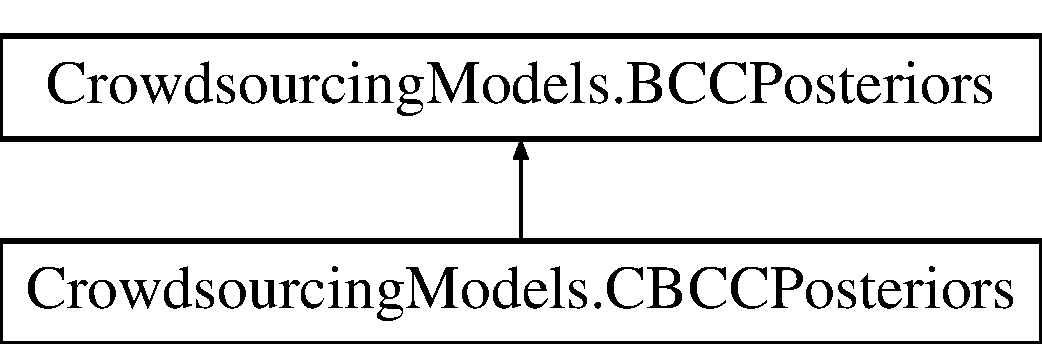
\includegraphics[height=2.000000cm]{class_crowdsourcing_models_1_1_c_b_c_c_posteriors}
\end{center}
\end{figure}
\subsection*{Public Attributes}
\begin{DoxyCompactItemize}
\item 
Dirichlet \hyperlink{class_crowdsourcing_models_1_1_c_b_c_c_posteriors_a5133c813b46dc47a1eca94f718c01560}{Community\+Prob}
\begin{DoxyCompactList}\small\item\em The Dirichlet posteriors of the workers community membership. \end{DoxyCompactList}\item 
Discrete\mbox{[}$\,$\mbox{]} \hyperlink{class_crowdsourcing_models_1_1_c_b_c_c_posteriors_ae0c96f63928949598cdd0051dc97c419}{Community}
\begin{DoxyCompactList}\small\item\em The posterior probabilities of the workers community membnerships. \end{DoxyCompactList}\item 
Dirichlet\mbox{[}$\,$\mbox{]}\mbox{[}$\,$\mbox{]} \hyperlink{class_crowdsourcing_models_1_1_c_b_c_c_posteriors_a66a61bd5cab64b9ada79b2ed55cf832a}{Community\+Confusion\+Matrix}
\begin{DoxyCompactList}\small\item\em The Dirichlet posteriors of the community confusion matrix. \end{DoxyCompactList}\item 
Vector\+Gaussian\mbox{[}$\,$\mbox{]}\mbox{[}$\,$\mbox{]} \hyperlink{class_crowdsourcing_models_1_1_c_b_c_c_posteriors_ad9a3f9c06a94f221a71bfa803f4b9434}{Community\+Score\+Matrix}
\begin{DoxyCompactList}\small\item\em The Gaussian posteriors of the community score matrix. \end{DoxyCompactList}\item 
Vector\+Gaussian\mbox{[}$\,$\mbox{]}\mbox{[}$\,$\mbox{]} \hyperlink{class_crowdsourcing_models_1_1_c_b_c_c_posteriors_a28a4852598eb85d4bc635c247d761f2b}{Worker\+Score\+Matrix\+Constraint}
\begin{DoxyCompactList}\small\item\em The Gaussian constraint of the community score matrix (used for online training). \end{DoxyCompactList}\item 
Discrete\mbox{[}$\,$\mbox{]} \hyperlink{class_crowdsourcing_models_1_1_c_b_c_c_posteriors_aa72e3388283ae2e52aaa15d232f38114}{Worker\+Community\+Constraint}
\begin{DoxyCompactList}\small\item\em Theconstraint of the workers community membership (used for online training). \end{DoxyCompactList}\end{DoxyCompactItemize}


\subsection{Detailed Description}
\hyperlink{class_crowdsourcing_models_1_1_c_b_c_c}{C\+B\+C\+C} posterior object. 



\subsection{Member Data Documentation}
\hypertarget{class_crowdsourcing_models_1_1_c_b_c_c_posteriors_ae0c96f63928949598cdd0051dc97c419}{}\index{Crowdsourcing\+Models\+::\+C\+B\+C\+C\+Posteriors@{Crowdsourcing\+Models\+::\+C\+B\+C\+C\+Posteriors}!Community@{Community}}
\index{Community@{Community}!Crowdsourcing\+Models\+::\+C\+B\+C\+C\+Posteriors@{Crowdsourcing\+Models\+::\+C\+B\+C\+C\+Posteriors}}
\subsubsection[{Community}]{\setlength{\rightskip}{0pt plus 5cm}Discrete \mbox{[}$\,$\mbox{]} Crowdsourcing\+Models.\+C\+B\+C\+C\+Posteriors.\+Community}\label{class_crowdsourcing_models_1_1_c_b_c_c_posteriors_ae0c96f63928949598cdd0051dc97c419}


The posterior probabilities of the workers community membnerships. 

\hypertarget{class_crowdsourcing_models_1_1_c_b_c_c_posteriors_a66a61bd5cab64b9ada79b2ed55cf832a}{}\index{Crowdsourcing\+Models\+::\+C\+B\+C\+C\+Posteriors@{Crowdsourcing\+Models\+::\+C\+B\+C\+C\+Posteriors}!Community\+Confusion\+Matrix@{Community\+Confusion\+Matrix}}
\index{Community\+Confusion\+Matrix@{Community\+Confusion\+Matrix}!Crowdsourcing\+Models\+::\+C\+B\+C\+C\+Posteriors@{Crowdsourcing\+Models\+::\+C\+B\+C\+C\+Posteriors}}
\subsubsection[{Community\+Confusion\+Matrix}]{\setlength{\rightskip}{0pt plus 5cm}Dirichlet \mbox{[}$\,$\mbox{]}\mbox{[}$\,$\mbox{]} Crowdsourcing\+Models.\+C\+B\+C\+C\+Posteriors.\+Community\+Confusion\+Matrix}\label{class_crowdsourcing_models_1_1_c_b_c_c_posteriors_a66a61bd5cab64b9ada79b2ed55cf832a}


The Dirichlet posteriors of the community confusion matrix. 

\hypertarget{class_crowdsourcing_models_1_1_c_b_c_c_posteriors_a5133c813b46dc47a1eca94f718c01560}{}\index{Crowdsourcing\+Models\+::\+C\+B\+C\+C\+Posteriors@{Crowdsourcing\+Models\+::\+C\+B\+C\+C\+Posteriors}!Community\+Prob@{Community\+Prob}}
\index{Community\+Prob@{Community\+Prob}!Crowdsourcing\+Models\+::\+C\+B\+C\+C\+Posteriors@{Crowdsourcing\+Models\+::\+C\+B\+C\+C\+Posteriors}}
\subsubsection[{Community\+Prob}]{\setlength{\rightskip}{0pt plus 5cm}Dirichlet Crowdsourcing\+Models.\+C\+B\+C\+C\+Posteriors.\+Community\+Prob}\label{class_crowdsourcing_models_1_1_c_b_c_c_posteriors_a5133c813b46dc47a1eca94f718c01560}


The Dirichlet posteriors of the workers community membership. 

\hypertarget{class_crowdsourcing_models_1_1_c_b_c_c_posteriors_ad9a3f9c06a94f221a71bfa803f4b9434}{}\index{Crowdsourcing\+Models\+::\+C\+B\+C\+C\+Posteriors@{Crowdsourcing\+Models\+::\+C\+B\+C\+C\+Posteriors}!Community\+Score\+Matrix@{Community\+Score\+Matrix}}
\index{Community\+Score\+Matrix@{Community\+Score\+Matrix}!Crowdsourcing\+Models\+::\+C\+B\+C\+C\+Posteriors@{Crowdsourcing\+Models\+::\+C\+B\+C\+C\+Posteriors}}
\subsubsection[{Community\+Score\+Matrix}]{\setlength{\rightskip}{0pt plus 5cm}Vector\+Gaussian \mbox{[}$\,$\mbox{]}\mbox{[}$\,$\mbox{]} Crowdsourcing\+Models.\+C\+B\+C\+C\+Posteriors.\+Community\+Score\+Matrix}\label{class_crowdsourcing_models_1_1_c_b_c_c_posteriors_ad9a3f9c06a94f221a71bfa803f4b9434}


The Gaussian posteriors of the community score matrix. 

\hypertarget{class_crowdsourcing_models_1_1_c_b_c_c_posteriors_aa72e3388283ae2e52aaa15d232f38114}{}\index{Crowdsourcing\+Models\+::\+C\+B\+C\+C\+Posteriors@{Crowdsourcing\+Models\+::\+C\+B\+C\+C\+Posteriors}!Worker\+Community\+Constraint@{Worker\+Community\+Constraint}}
\index{Worker\+Community\+Constraint@{Worker\+Community\+Constraint}!Crowdsourcing\+Models\+::\+C\+B\+C\+C\+Posteriors@{Crowdsourcing\+Models\+::\+C\+B\+C\+C\+Posteriors}}
\subsubsection[{Worker\+Community\+Constraint}]{\setlength{\rightskip}{0pt plus 5cm}Discrete \mbox{[}$\,$\mbox{]} Crowdsourcing\+Models.\+C\+B\+C\+C\+Posteriors.\+Worker\+Community\+Constraint}\label{class_crowdsourcing_models_1_1_c_b_c_c_posteriors_aa72e3388283ae2e52aaa15d232f38114}


Theconstraint of the workers community membership (used for online training). 

\hypertarget{class_crowdsourcing_models_1_1_c_b_c_c_posteriors_a28a4852598eb85d4bc635c247d761f2b}{}\index{Crowdsourcing\+Models\+::\+C\+B\+C\+C\+Posteriors@{Crowdsourcing\+Models\+::\+C\+B\+C\+C\+Posteriors}!Worker\+Score\+Matrix\+Constraint@{Worker\+Score\+Matrix\+Constraint}}
\index{Worker\+Score\+Matrix\+Constraint@{Worker\+Score\+Matrix\+Constraint}!Crowdsourcing\+Models\+::\+C\+B\+C\+C\+Posteriors@{Crowdsourcing\+Models\+::\+C\+B\+C\+C\+Posteriors}}
\subsubsection[{Worker\+Score\+Matrix\+Constraint}]{\setlength{\rightskip}{0pt plus 5cm}Vector\+Gaussian \mbox{[}$\,$\mbox{]}\mbox{[}$\,$\mbox{]} Crowdsourcing\+Models.\+C\+B\+C\+C\+Posteriors.\+Worker\+Score\+Matrix\+Constraint}\label{class_crowdsourcing_models_1_1_c_b_c_c_posteriors_a28a4852598eb85d4bc635c247d761f2b}


The Gaussian constraint of the community score matrix (used for online training). 



The documentation for this class was generated from the following file\+:\begin{DoxyCompactItemize}
\item 
C\+:/\+Users/\+Matteo/\+Source/\+Repos/active-\/crowd/\+Crowdsourcing\+Models/C\+B\+C\+C.\+cs\end{DoxyCompactItemize}

\hypertarget{class_crowdsourcing_project_1_1_statistics_1_1_confusion_matrix}{}\section{Crowdsourcing\+Project.\+Statistics.\+Confusion\+Matrix Class Reference}
\label{class_crowdsourcing_project_1_1_statistics_1_1_confusion_matrix}\index{Crowdsourcing\+Project.\+Statistics.\+Confusion\+Matrix@{Crowdsourcing\+Project.\+Statistics.\+Confusion\+Matrix}}


Confusion Matrix class  


Inheritance diagram for Crowdsourcing\+Project.\+Statistics.\+Confusion\+Matrix\+:\begin{figure}[H]
\begin{center}
\leavevmode
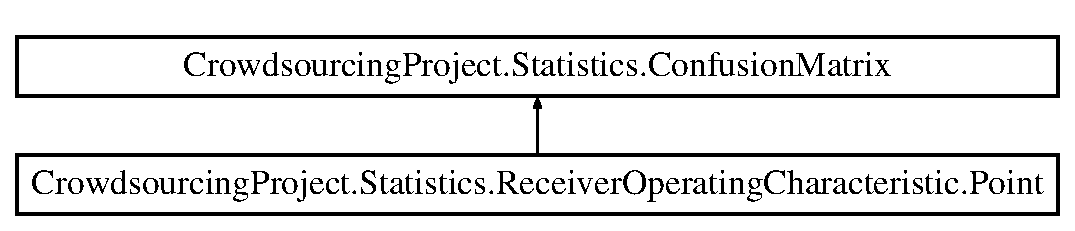
\includegraphics[height=2.000000cm]{class_crowdsourcing_project_1_1_statistics_1_1_confusion_matrix}
\end{center}
\end{figure}
\subsection*{Public Member Functions}
\begin{DoxyCompactItemize}
\item 
\hyperlink{class_crowdsourcing_project_1_1_statistics_1_1_confusion_matrix_add656d4ea4928b25ef16b0a35cba6f90}{Confusion\+Matrix} (int true\+Positives, int true\+Negatives, int false\+Positives, int false\+Negatives)
\begin{DoxyCompactList}\small\item\em Constructs a new Confusion Matrix. \end{DoxyCompactList}\end{DoxyCompactItemize}
\subsection*{Properties}
\begin{DoxyCompactItemize}
\item 
int \hyperlink{class_crowdsourcing_project_1_1_statistics_1_1_confusion_matrix_a9f421cb6ea3fab10b50af5c05e663146}{Observations}\hspace{0.3cm}{\ttfamily  \mbox{[}get\mbox{]}}
\begin{DoxyCompactList}\small\item\em Gets the number of observations for this matrix \end{DoxyCompactList}\item 
int \hyperlink{class_crowdsourcing_project_1_1_statistics_1_1_confusion_matrix_a5e9d3164713343c5fb0b2181247c6629}{Actual\+Positives}\hspace{0.3cm}{\ttfamily  \mbox{[}get\mbox{]}}
\begin{DoxyCompactList}\small\item\em Gets the number of actual positives \end{DoxyCompactList}\item 
int \hyperlink{class_crowdsourcing_project_1_1_statistics_1_1_confusion_matrix_ac0499cbf491c53f963cef98c734e036e}{Actual\+Negatives}\hspace{0.3cm}{\ttfamily  \mbox{[}get\mbox{]}}
\begin{DoxyCompactList}\small\item\em Gets the number of actual negatives \end{DoxyCompactList}\item 
int \hyperlink{class_crowdsourcing_project_1_1_statistics_1_1_confusion_matrix_a4e5867d4530373feab1bc0bedbb116c6}{Predicted\+Positives}\hspace{0.3cm}{\ttfamily  \mbox{[}get\mbox{]}}
\begin{DoxyCompactList}\small\item\em Gets the number of predicted positives \end{DoxyCompactList}\item 
int \hyperlink{class_crowdsourcing_project_1_1_statistics_1_1_confusion_matrix_a3206bbbeb0b665b1b597bd02d21a3b07}{Predicted\+Negatives}\hspace{0.3cm}{\ttfamily  \mbox{[}get\mbox{]}}
\begin{DoxyCompactList}\small\item\em Gets the number of predicted negatives \end{DoxyCompactList}\item 
int \hyperlink{class_crowdsourcing_project_1_1_statistics_1_1_confusion_matrix_ae1776127573af2d851e6102bb71acc30}{True\+Positives}\hspace{0.3cm}{\ttfamily  \mbox{[}get\mbox{]}}
\begin{DoxyCompactList}\small\item\em Cases correctly identified by the system as positives. \end{DoxyCompactList}\item 
int \hyperlink{class_crowdsourcing_project_1_1_statistics_1_1_confusion_matrix_a76af45bf60135f1f3d6cf64392be49c8}{True\+Negatives}\hspace{0.3cm}{\ttfamily  \mbox{[}get\mbox{]}}
\begin{DoxyCompactList}\small\item\em Cases correctly identified by the system as negatives. \end{DoxyCompactList}\item 
int \hyperlink{class_crowdsourcing_project_1_1_statistics_1_1_confusion_matrix_accb022837853f2f22fcd610aa5379c0e}{False\+Positives}\hspace{0.3cm}{\ttfamily  \mbox{[}get\mbox{]}}
\begin{DoxyCompactList}\small\item\em Cases incorrectly identified by the system as positives. \end{DoxyCompactList}\item 
int \hyperlink{class_crowdsourcing_project_1_1_statistics_1_1_confusion_matrix_a6e681408fc24887a2f64f711de077fe6}{False\+Negatives}\hspace{0.3cm}{\ttfamily  \mbox{[}get\mbox{]}}
\begin{DoxyCompactList}\small\item\em Cases incorrectly identified by the system as negatives. \end{DoxyCompactList}\item 
double \hyperlink{class_crowdsourcing_project_1_1_statistics_1_1_confusion_matrix_ac8c37fcc9f7bc87122cfb030ef4039a1}{Sensitivity}\hspace{0.3cm}{\ttfamily  \mbox{[}get\mbox{]}}
\begin{DoxyCompactList}\small\item\em Sensitivity, also known as True Positive Rate \end{DoxyCompactList}\item 
double \hyperlink{class_crowdsourcing_project_1_1_statistics_1_1_confusion_matrix_a214f269cbfeb96d7e50f013fd8e64c5c}{Specificity}\hspace{0.3cm}{\ttfamily  \mbox{[}get\mbox{]}}
\begin{DoxyCompactList}\small\item\em Specificity, also known as True Negative Rate \end{DoxyCompactList}\item 
double \hyperlink{class_crowdsourcing_project_1_1_statistics_1_1_confusion_matrix_a3450802726f22c62f6fbdf97e42451a8}{Efficiency}\hspace{0.3cm}{\ttfamily  \mbox{[}get\mbox{]}}
\begin{DoxyCompactList}\small\item\em Efficiency, the arithmetic mean of sensitivity and specificity \end{DoxyCompactList}\item 
double \hyperlink{class_crowdsourcing_project_1_1_statistics_1_1_confusion_matrix_a6cc65bbd56a6e577d4bae7650bab3897}{Accuracy}\hspace{0.3cm}{\ttfamily  \mbox{[}get\mbox{]}}
\begin{DoxyCompactList}\small\item\em Accuracy, or raw performance of the system \end{DoxyCompactList}\item 
double \hyperlink{class_crowdsourcing_project_1_1_statistics_1_1_confusion_matrix_afb699f40850b19bba5c430eab686eff2}{Positive\+Predictive\+Value}\hspace{0.3cm}{\ttfamily  \mbox{[}get\mbox{]}}
\begin{DoxyCompactList}\small\item\em Positive Predictive Value, also known as Positive Precision \end{DoxyCompactList}\item 
double \hyperlink{class_crowdsourcing_project_1_1_statistics_1_1_confusion_matrix_a53e260e21777e62a8880d57ae1a2d6b4}{Negative\+Predictive\+Value}\hspace{0.3cm}{\ttfamily  \mbox{[}get\mbox{]}}
\begin{DoxyCompactList}\small\item\em Negative Predictive Value, also known as Negative Precision \end{DoxyCompactList}\item 
double \hyperlink{class_crowdsourcing_project_1_1_statistics_1_1_confusion_matrix_a883fcaefecb1086c5931cd870c2ef4b1}{False\+Positive\+Rate}\hspace{0.3cm}{\ttfamily  \mbox{[}get\mbox{]}}
\begin{DoxyCompactList}\small\item\em False Positive Rate, also known as false alarm rate. \end{DoxyCompactList}\item 
double \hyperlink{class_crowdsourcing_project_1_1_statistics_1_1_confusion_matrix_a9cd513ee90fdf9d5746baf59a219725b}{False\+Discovery\+Rate}\hspace{0.3cm}{\ttfamily  \mbox{[}get\mbox{]}}
\begin{DoxyCompactList}\small\item\em False Discovery Rate, or the expected false positive rate. \end{DoxyCompactList}\item 
double \hyperlink{class_crowdsourcing_project_1_1_statistics_1_1_confusion_matrix_a6f7ebbf52b5ef320df88d4e5eba8ab4a}{Matthews\+Correlation\+Coefficient}\hspace{0.3cm}{\ttfamily  \mbox{[}get\mbox{]}}
\begin{DoxyCompactList}\small\item\em Matthews Correlation Coefficient, also known as Phi coefficient \end{DoxyCompactList}\end{DoxyCompactItemize}


\subsection{Detailed Description}
Confusion Matrix class 



\subsection{Constructor \& Destructor Documentation}
\hypertarget{class_crowdsourcing_project_1_1_statistics_1_1_confusion_matrix_add656d4ea4928b25ef16b0a35cba6f90}{}\index{Crowdsourcing\+Project\+::\+Statistics\+::\+Confusion\+Matrix@{Crowdsourcing\+Project\+::\+Statistics\+::\+Confusion\+Matrix}!Confusion\+Matrix@{Confusion\+Matrix}}
\index{Confusion\+Matrix@{Confusion\+Matrix}!Crowdsourcing\+Project\+::\+Statistics\+::\+Confusion\+Matrix@{Crowdsourcing\+Project\+::\+Statistics\+::\+Confusion\+Matrix}}
\subsubsection[{Confusion\+Matrix(int true\+Positives, int true\+Negatives, int false\+Positives, int false\+Negatives)}]{\setlength{\rightskip}{0pt plus 5cm}Crowdsourcing\+Project.\+Statistics.\+Confusion\+Matrix.\+Confusion\+Matrix (
\begin{DoxyParamCaption}
\item[{int}]{true\+Positives, }
\item[{int}]{true\+Negatives, }
\item[{int}]{false\+Positives, }
\item[{int}]{false\+Negatives}
\end{DoxyParamCaption}
)\hspace{0.3cm}{\ttfamily [inline]}}\label{class_crowdsourcing_project_1_1_statistics_1_1_confusion_matrix_add656d4ea4928b25ef16b0a35cba6f90}


Constructs a new Confusion Matrix. 



\subsection{Property Documentation}
\hypertarget{class_crowdsourcing_project_1_1_statistics_1_1_confusion_matrix_a6cc65bbd56a6e577d4bae7650bab3897}{}\index{Crowdsourcing\+Project\+::\+Statistics\+::\+Confusion\+Matrix@{Crowdsourcing\+Project\+::\+Statistics\+::\+Confusion\+Matrix}!Accuracy@{Accuracy}}
\index{Accuracy@{Accuracy}!Crowdsourcing\+Project\+::\+Statistics\+::\+Confusion\+Matrix@{Crowdsourcing\+Project\+::\+Statistics\+::\+Confusion\+Matrix}}
\subsubsection[{Accuracy}]{\setlength{\rightskip}{0pt plus 5cm}double Crowdsourcing\+Project.\+Statistics.\+Confusion\+Matrix.\+Accuracy\hspace{0.3cm}{\ttfamily [get]}}\label{class_crowdsourcing_project_1_1_statistics_1_1_confusion_matrix_a6cc65bbd56a6e577d4bae7650bab3897}


Accuracy, or raw performance of the system 

A\+C\+C = (T\+P + T\+N) / (P + N) \hypertarget{class_crowdsourcing_project_1_1_statistics_1_1_confusion_matrix_ac0499cbf491c53f963cef98c734e036e}{}\index{Crowdsourcing\+Project\+::\+Statistics\+::\+Confusion\+Matrix@{Crowdsourcing\+Project\+::\+Statistics\+::\+Confusion\+Matrix}!Actual\+Negatives@{Actual\+Negatives}}
\index{Actual\+Negatives@{Actual\+Negatives}!Crowdsourcing\+Project\+::\+Statistics\+::\+Confusion\+Matrix@{Crowdsourcing\+Project\+::\+Statistics\+::\+Confusion\+Matrix}}
\subsubsection[{Actual\+Negatives}]{\setlength{\rightskip}{0pt plus 5cm}int Crowdsourcing\+Project.\+Statistics.\+Confusion\+Matrix.\+Actual\+Negatives\hspace{0.3cm}{\ttfamily [get]}}\label{class_crowdsourcing_project_1_1_statistics_1_1_confusion_matrix_ac0499cbf491c53f963cef98c734e036e}


Gets the number of actual negatives 

\hypertarget{class_crowdsourcing_project_1_1_statistics_1_1_confusion_matrix_a5e9d3164713343c5fb0b2181247c6629}{}\index{Crowdsourcing\+Project\+::\+Statistics\+::\+Confusion\+Matrix@{Crowdsourcing\+Project\+::\+Statistics\+::\+Confusion\+Matrix}!Actual\+Positives@{Actual\+Positives}}
\index{Actual\+Positives@{Actual\+Positives}!Crowdsourcing\+Project\+::\+Statistics\+::\+Confusion\+Matrix@{Crowdsourcing\+Project\+::\+Statistics\+::\+Confusion\+Matrix}}
\subsubsection[{Actual\+Positives}]{\setlength{\rightskip}{0pt plus 5cm}int Crowdsourcing\+Project.\+Statistics.\+Confusion\+Matrix.\+Actual\+Positives\hspace{0.3cm}{\ttfamily [get]}}\label{class_crowdsourcing_project_1_1_statistics_1_1_confusion_matrix_a5e9d3164713343c5fb0b2181247c6629}


Gets the number of actual positives 

\hypertarget{class_crowdsourcing_project_1_1_statistics_1_1_confusion_matrix_a3450802726f22c62f6fbdf97e42451a8}{}\index{Crowdsourcing\+Project\+::\+Statistics\+::\+Confusion\+Matrix@{Crowdsourcing\+Project\+::\+Statistics\+::\+Confusion\+Matrix}!Efficiency@{Efficiency}}
\index{Efficiency@{Efficiency}!Crowdsourcing\+Project\+::\+Statistics\+::\+Confusion\+Matrix@{Crowdsourcing\+Project\+::\+Statistics\+::\+Confusion\+Matrix}}
\subsubsection[{Efficiency}]{\setlength{\rightskip}{0pt plus 5cm}double Crowdsourcing\+Project.\+Statistics.\+Confusion\+Matrix.\+Efficiency\hspace{0.3cm}{\ttfamily [get]}}\label{class_crowdsourcing_project_1_1_statistics_1_1_confusion_matrix_a3450802726f22c62f6fbdf97e42451a8}


Efficiency, the arithmetic mean of sensitivity and specificity 

\hypertarget{class_crowdsourcing_project_1_1_statistics_1_1_confusion_matrix_a9cd513ee90fdf9d5746baf59a219725b}{}\index{Crowdsourcing\+Project\+::\+Statistics\+::\+Confusion\+Matrix@{Crowdsourcing\+Project\+::\+Statistics\+::\+Confusion\+Matrix}!False\+Discovery\+Rate@{False\+Discovery\+Rate}}
\index{False\+Discovery\+Rate@{False\+Discovery\+Rate}!Crowdsourcing\+Project\+::\+Statistics\+::\+Confusion\+Matrix@{Crowdsourcing\+Project\+::\+Statistics\+::\+Confusion\+Matrix}}
\subsubsection[{False\+Discovery\+Rate}]{\setlength{\rightskip}{0pt plus 5cm}double Crowdsourcing\+Project.\+Statistics.\+Confusion\+Matrix.\+False\+Discovery\+Rate\hspace{0.3cm}{\ttfamily [get]}}\label{class_crowdsourcing_project_1_1_statistics_1_1_confusion_matrix_a9cd513ee90fdf9d5746baf59a219725b}


False Discovery Rate, or the expected false positive rate. 

The False Discovery Rate is actually the expected false positive rate.

For example, if 1000 observations were experimentally predicted to be different, and a maximum F\+D\+R for these observations was 0.\+10, then 100 of these observations would be expected to be false positives.

It is calculated as\+: F\+D\+R = F\+P / (F\+P + T\+P) \hypertarget{class_crowdsourcing_project_1_1_statistics_1_1_confusion_matrix_a6e681408fc24887a2f64f711de077fe6}{}\index{Crowdsourcing\+Project\+::\+Statistics\+::\+Confusion\+Matrix@{Crowdsourcing\+Project\+::\+Statistics\+::\+Confusion\+Matrix}!False\+Negatives@{False\+Negatives}}
\index{False\+Negatives@{False\+Negatives}!Crowdsourcing\+Project\+::\+Statistics\+::\+Confusion\+Matrix@{Crowdsourcing\+Project\+::\+Statistics\+::\+Confusion\+Matrix}}
\subsubsection[{False\+Negatives}]{\setlength{\rightskip}{0pt plus 5cm}int Crowdsourcing\+Project.\+Statistics.\+Confusion\+Matrix.\+False\+Negatives\hspace{0.3cm}{\ttfamily [get]}}\label{class_crowdsourcing_project_1_1_statistics_1_1_confusion_matrix_a6e681408fc24887a2f64f711de077fe6}


Cases incorrectly identified by the system as negatives. 

\hypertarget{class_crowdsourcing_project_1_1_statistics_1_1_confusion_matrix_a883fcaefecb1086c5931cd870c2ef4b1}{}\index{Crowdsourcing\+Project\+::\+Statistics\+::\+Confusion\+Matrix@{Crowdsourcing\+Project\+::\+Statistics\+::\+Confusion\+Matrix}!False\+Positive\+Rate@{False\+Positive\+Rate}}
\index{False\+Positive\+Rate@{False\+Positive\+Rate}!Crowdsourcing\+Project\+::\+Statistics\+::\+Confusion\+Matrix@{Crowdsourcing\+Project\+::\+Statistics\+::\+Confusion\+Matrix}}
\subsubsection[{False\+Positive\+Rate}]{\setlength{\rightskip}{0pt plus 5cm}double Crowdsourcing\+Project.\+Statistics.\+Confusion\+Matrix.\+False\+Positive\+Rate\hspace{0.3cm}{\ttfamily [get]}}\label{class_crowdsourcing_project_1_1_statistics_1_1_confusion_matrix_a883fcaefecb1086c5931cd870c2ef4b1}


False Positive Rate, also known as false alarm rate. 

It can be calculated as\+: F\+P\+R = F\+P / (F\+P + T\+N) or also as\+: F\+P\+R = (1-\/specifity) \hypertarget{class_crowdsourcing_project_1_1_statistics_1_1_confusion_matrix_accb022837853f2f22fcd610aa5379c0e}{}\index{Crowdsourcing\+Project\+::\+Statistics\+::\+Confusion\+Matrix@{Crowdsourcing\+Project\+::\+Statistics\+::\+Confusion\+Matrix}!False\+Positives@{False\+Positives}}
\index{False\+Positives@{False\+Positives}!Crowdsourcing\+Project\+::\+Statistics\+::\+Confusion\+Matrix@{Crowdsourcing\+Project\+::\+Statistics\+::\+Confusion\+Matrix}}
\subsubsection[{False\+Positives}]{\setlength{\rightskip}{0pt plus 5cm}int Crowdsourcing\+Project.\+Statistics.\+Confusion\+Matrix.\+False\+Positives\hspace{0.3cm}{\ttfamily [get]}}\label{class_crowdsourcing_project_1_1_statistics_1_1_confusion_matrix_accb022837853f2f22fcd610aa5379c0e}


Cases incorrectly identified by the system as positives. 

\hypertarget{class_crowdsourcing_project_1_1_statistics_1_1_confusion_matrix_a6f7ebbf52b5ef320df88d4e5eba8ab4a}{}\index{Crowdsourcing\+Project\+::\+Statistics\+::\+Confusion\+Matrix@{Crowdsourcing\+Project\+::\+Statistics\+::\+Confusion\+Matrix}!Matthews\+Correlation\+Coefficient@{Matthews\+Correlation\+Coefficient}}
\index{Matthews\+Correlation\+Coefficient@{Matthews\+Correlation\+Coefficient}!Crowdsourcing\+Project\+::\+Statistics\+::\+Confusion\+Matrix@{Crowdsourcing\+Project\+::\+Statistics\+::\+Confusion\+Matrix}}
\subsubsection[{Matthews\+Correlation\+Coefficient}]{\setlength{\rightskip}{0pt plus 5cm}double Crowdsourcing\+Project.\+Statistics.\+Confusion\+Matrix.\+Matthews\+Correlation\+Coefficient\hspace{0.3cm}{\ttfamily [get]}}\label{class_crowdsourcing_project_1_1_statistics_1_1_confusion_matrix_a6f7ebbf52b5ef320df88d4e5eba8ab4a}


Matthews Correlation Coefficient, also known as Phi coefficient 

A coefficient of +1 represents a perfect prediction, 0 an average random prediction and −1 an inverse prediction. \hypertarget{class_crowdsourcing_project_1_1_statistics_1_1_confusion_matrix_a53e260e21777e62a8880d57ae1a2d6b4}{}\index{Crowdsourcing\+Project\+::\+Statistics\+::\+Confusion\+Matrix@{Crowdsourcing\+Project\+::\+Statistics\+::\+Confusion\+Matrix}!Negative\+Predictive\+Value@{Negative\+Predictive\+Value}}
\index{Negative\+Predictive\+Value@{Negative\+Predictive\+Value}!Crowdsourcing\+Project\+::\+Statistics\+::\+Confusion\+Matrix@{Crowdsourcing\+Project\+::\+Statistics\+::\+Confusion\+Matrix}}
\subsubsection[{Negative\+Predictive\+Value}]{\setlength{\rightskip}{0pt plus 5cm}double Crowdsourcing\+Project.\+Statistics.\+Confusion\+Matrix.\+Negative\+Predictive\+Value\hspace{0.3cm}{\ttfamily [get]}}\label{class_crowdsourcing_project_1_1_statistics_1_1_confusion_matrix_a53e260e21777e62a8880d57ae1a2d6b4}


Negative Predictive Value, also known as Negative Precision 

The Negative Predictive Value tells us how likely it is that the disease is N\+O\+T present for a patient, given that the patient\textquotesingle{}s test for the disease is negative.

It can be calculated as\+: N\+P\+V = T\+N / (T\+N + F\+N) \hypertarget{class_crowdsourcing_project_1_1_statistics_1_1_confusion_matrix_a9f421cb6ea3fab10b50af5c05e663146}{}\index{Crowdsourcing\+Project\+::\+Statistics\+::\+Confusion\+Matrix@{Crowdsourcing\+Project\+::\+Statistics\+::\+Confusion\+Matrix}!Observations@{Observations}}
\index{Observations@{Observations}!Crowdsourcing\+Project\+::\+Statistics\+::\+Confusion\+Matrix@{Crowdsourcing\+Project\+::\+Statistics\+::\+Confusion\+Matrix}}
\subsubsection[{Observations}]{\setlength{\rightskip}{0pt plus 5cm}int Crowdsourcing\+Project.\+Statistics.\+Confusion\+Matrix.\+Observations\hspace{0.3cm}{\ttfamily [get]}}\label{class_crowdsourcing_project_1_1_statistics_1_1_confusion_matrix_a9f421cb6ea3fab10b50af5c05e663146}


Gets the number of observations for this matrix 

\hypertarget{class_crowdsourcing_project_1_1_statistics_1_1_confusion_matrix_afb699f40850b19bba5c430eab686eff2}{}\index{Crowdsourcing\+Project\+::\+Statistics\+::\+Confusion\+Matrix@{Crowdsourcing\+Project\+::\+Statistics\+::\+Confusion\+Matrix}!Positive\+Predictive\+Value@{Positive\+Predictive\+Value}}
\index{Positive\+Predictive\+Value@{Positive\+Predictive\+Value}!Crowdsourcing\+Project\+::\+Statistics\+::\+Confusion\+Matrix@{Crowdsourcing\+Project\+::\+Statistics\+::\+Confusion\+Matrix}}
\subsubsection[{Positive\+Predictive\+Value}]{\setlength{\rightskip}{0pt plus 5cm}double Crowdsourcing\+Project.\+Statistics.\+Confusion\+Matrix.\+Positive\+Predictive\+Value\hspace{0.3cm}{\ttfamily [get]}}\label{class_crowdsourcing_project_1_1_statistics_1_1_confusion_matrix_afb699f40850b19bba5c430eab686eff2}


Positive Predictive Value, also known as Positive Precision 

The Positive Predictive Value tells us how likely is that a patient has a disease, given that the test for this disease is positive.

It can be calculated as\+: P\+P\+V = T\+P / (T\+P + F\+P) \hypertarget{class_crowdsourcing_project_1_1_statistics_1_1_confusion_matrix_a3206bbbeb0b665b1b597bd02d21a3b07}{}\index{Crowdsourcing\+Project\+::\+Statistics\+::\+Confusion\+Matrix@{Crowdsourcing\+Project\+::\+Statistics\+::\+Confusion\+Matrix}!Predicted\+Negatives@{Predicted\+Negatives}}
\index{Predicted\+Negatives@{Predicted\+Negatives}!Crowdsourcing\+Project\+::\+Statistics\+::\+Confusion\+Matrix@{Crowdsourcing\+Project\+::\+Statistics\+::\+Confusion\+Matrix}}
\subsubsection[{Predicted\+Negatives}]{\setlength{\rightskip}{0pt plus 5cm}int Crowdsourcing\+Project.\+Statistics.\+Confusion\+Matrix.\+Predicted\+Negatives\hspace{0.3cm}{\ttfamily [get]}}\label{class_crowdsourcing_project_1_1_statistics_1_1_confusion_matrix_a3206bbbeb0b665b1b597bd02d21a3b07}


Gets the number of predicted negatives 

\hypertarget{class_crowdsourcing_project_1_1_statistics_1_1_confusion_matrix_a4e5867d4530373feab1bc0bedbb116c6}{}\index{Crowdsourcing\+Project\+::\+Statistics\+::\+Confusion\+Matrix@{Crowdsourcing\+Project\+::\+Statistics\+::\+Confusion\+Matrix}!Predicted\+Positives@{Predicted\+Positives}}
\index{Predicted\+Positives@{Predicted\+Positives}!Crowdsourcing\+Project\+::\+Statistics\+::\+Confusion\+Matrix@{Crowdsourcing\+Project\+::\+Statistics\+::\+Confusion\+Matrix}}
\subsubsection[{Predicted\+Positives}]{\setlength{\rightskip}{0pt plus 5cm}int Crowdsourcing\+Project.\+Statistics.\+Confusion\+Matrix.\+Predicted\+Positives\hspace{0.3cm}{\ttfamily [get]}}\label{class_crowdsourcing_project_1_1_statistics_1_1_confusion_matrix_a4e5867d4530373feab1bc0bedbb116c6}


Gets the number of predicted positives 

\hypertarget{class_crowdsourcing_project_1_1_statistics_1_1_confusion_matrix_ac8c37fcc9f7bc87122cfb030ef4039a1}{}\index{Crowdsourcing\+Project\+::\+Statistics\+::\+Confusion\+Matrix@{Crowdsourcing\+Project\+::\+Statistics\+::\+Confusion\+Matrix}!Sensitivity@{Sensitivity}}
\index{Sensitivity@{Sensitivity}!Crowdsourcing\+Project\+::\+Statistics\+::\+Confusion\+Matrix@{Crowdsourcing\+Project\+::\+Statistics\+::\+Confusion\+Matrix}}
\subsubsection[{Sensitivity}]{\setlength{\rightskip}{0pt plus 5cm}double Crowdsourcing\+Project.\+Statistics.\+Confusion\+Matrix.\+Sensitivity\hspace{0.3cm}{\ttfamily [get]}}\label{class_crowdsourcing_project_1_1_statistics_1_1_confusion_matrix_ac8c37fcc9f7bc87122cfb030ef4039a1}


Sensitivity, also known as True Positive Rate 

Sensitivity = T\+P\+R = T\+P / (T\+P + F\+N) \hypertarget{class_crowdsourcing_project_1_1_statistics_1_1_confusion_matrix_a214f269cbfeb96d7e50f013fd8e64c5c}{}\index{Crowdsourcing\+Project\+::\+Statistics\+::\+Confusion\+Matrix@{Crowdsourcing\+Project\+::\+Statistics\+::\+Confusion\+Matrix}!Specificity@{Specificity}}
\index{Specificity@{Specificity}!Crowdsourcing\+Project\+::\+Statistics\+::\+Confusion\+Matrix@{Crowdsourcing\+Project\+::\+Statistics\+::\+Confusion\+Matrix}}
\subsubsection[{Specificity}]{\setlength{\rightskip}{0pt plus 5cm}double Crowdsourcing\+Project.\+Statistics.\+Confusion\+Matrix.\+Specificity\hspace{0.3cm}{\ttfamily [get]}}\label{class_crowdsourcing_project_1_1_statistics_1_1_confusion_matrix_a214f269cbfeb96d7e50f013fd8e64c5c}


Specificity, also known as True Negative Rate 

Specificity = T\+N\+R = T\+N / (F\+P + T\+N) or also as\+: T\+N\+R = (1-\/\+False Positive Rate) \hypertarget{class_crowdsourcing_project_1_1_statistics_1_1_confusion_matrix_a76af45bf60135f1f3d6cf64392be49c8}{}\index{Crowdsourcing\+Project\+::\+Statistics\+::\+Confusion\+Matrix@{Crowdsourcing\+Project\+::\+Statistics\+::\+Confusion\+Matrix}!True\+Negatives@{True\+Negatives}}
\index{True\+Negatives@{True\+Negatives}!Crowdsourcing\+Project\+::\+Statistics\+::\+Confusion\+Matrix@{Crowdsourcing\+Project\+::\+Statistics\+::\+Confusion\+Matrix}}
\subsubsection[{True\+Negatives}]{\setlength{\rightskip}{0pt plus 5cm}int Crowdsourcing\+Project.\+Statistics.\+Confusion\+Matrix.\+True\+Negatives\hspace{0.3cm}{\ttfamily [get]}}\label{class_crowdsourcing_project_1_1_statistics_1_1_confusion_matrix_a76af45bf60135f1f3d6cf64392be49c8}


Cases correctly identified by the system as negatives. 

\hypertarget{class_crowdsourcing_project_1_1_statistics_1_1_confusion_matrix_ae1776127573af2d851e6102bb71acc30}{}\index{Crowdsourcing\+Project\+::\+Statistics\+::\+Confusion\+Matrix@{Crowdsourcing\+Project\+::\+Statistics\+::\+Confusion\+Matrix}!True\+Positives@{True\+Positives}}
\index{True\+Positives@{True\+Positives}!Crowdsourcing\+Project\+::\+Statistics\+::\+Confusion\+Matrix@{Crowdsourcing\+Project\+::\+Statistics\+::\+Confusion\+Matrix}}
\subsubsection[{True\+Positives}]{\setlength{\rightskip}{0pt plus 5cm}int Crowdsourcing\+Project.\+Statistics.\+Confusion\+Matrix.\+True\+Positives\hspace{0.3cm}{\ttfamily [get]}}\label{class_crowdsourcing_project_1_1_statistics_1_1_confusion_matrix_ae1776127573af2d851e6102bb71acc30}


Cases correctly identified by the system as positives. 



The documentation for this class was generated from the following file\+:\begin{DoxyCompactItemize}
\item 
C\+:/\+Users/\+Matteo/\+Source/\+Repos/active-\/crowd/\+Crowdsourcing\+Models/\+Statistics/Confusion\+Matrix.\+cs\end{DoxyCompactItemize}

\hypertarget{class_crowdsourcing_models_1_1_data_mapping}{}\section{Crowdsourcing\+Models.\+Data\+Mapping Class Reference}
\label{class_crowdsourcing_models_1_1_data_mapping}\index{Crowdsourcing\+Models.\+Data\+Mapping@{Crowdsourcing\+Models.\+Data\+Mapping}}


Data mapping class. This class manages the mapping between the data (which is in the form of task, worker ids, and labels) and the model data (which is in term of indices).  


\subsection*{Public Member Functions}
\begin{DoxyCompactItemize}
\item 
\hyperlink{class_crowdsourcing_models_1_1_data_mapping_aeb425a824cc4074db2857ac8ba6c1a69}{Data\+Mapping} (I\+Enumerable$<$ \hyperlink{class_crowdsourcing_models_1_1_datum}{Datum} $>$ data, int num\+Communities=-\/1, int label\+Min=int.\+Max\+Value, int label\+Max=int.\+Min\+Value)
\begin{DoxyCompactList}\small\item\em Creates a data mapping. \end{DoxyCompactList}\item 
int\mbox{[}$\,$\mbox{]}\mbox{[}$\,$\mbox{]} \hyperlink{class_crowdsourcing_models_1_1_data_mapping_a1d48c08325772a613b78f4a8a52c57e9}{Get\+Task\+Indices\+Per\+Worker\+Index} (I\+Enumerable$<$ \hyperlink{class_crowdsourcing_models_1_1_datum}{Datum} $>$ data)
\begin{DoxyCompactList}\small\item\em Returns the matrix of the task indices (columns) of each worker (rows). \end{DoxyCompactList}\item 
int\mbox{[}$\,$\mbox{]}\mbox{[}$\,$\mbox{]} \hyperlink{class_crowdsourcing_models_1_1_data_mapping_ad7a6b996ec247265bc7902b9e48d0c3d}{Get\+Labels\+Per\+Worker\+Index} (I\+Enumerable$<$ \hyperlink{class_crowdsourcing_models_1_1_datum}{Datum} $>$ data)
\begin{DoxyCompactList}\small\item\em Returns the matrix of the labels (columns) of each worker (rows). \end{DoxyCompactList}\item 
Dictionary$<$ string, int?$>$ \hyperlink{class_crowdsourcing_models_1_1_data_mapping_ad542e9c734bb68b141e7cb24f9236196}{Get\+Gold\+Labels\+Per\+Task\+Id} ()
\begin{DoxyCompactList}\small\item\em Returns the the gold labels of each task. \end{DoxyCompactList}\item 
\hypertarget{class_crowdsourcing_models_1_1_data_mapping_af69c3292c1b9522772007cc8433b1330}{}Dictionary$<$ string, int?$>$ {\bfseries Get\+Random\+Label\+Per\+Task\+Id} (I\+List$<$ \hyperlink{class_crowdsourcing_models_1_1_datum}{Datum} $>$ data)\label{class_crowdsourcing_models_1_1_data_mapping_af69c3292c1b9522772007cc8433b1330}

\item 
\hypertarget{class_crowdsourcing_models_1_1_data_mapping_ae52e28d46739ddf659e671b189a9d6a9}{}int\mbox{[}$\,$\mbox{]} {\bfseries Get\+Gold\+Labels\+Per\+Task\+Index} ()\label{class_crowdsourcing_models_1_1_data_mapping_ae52e28d46739ddf659e671b189a9d6a9}

\item 
\hypertarget{class_crowdsourcing_models_1_1_data_mapping_a93a884e4f60d956db1722e80ad3aeda2}{}double\mbox{[}$\,$\mbox{]}\mbox{[}$\,$\mbox{]} {\bfseries Get\+Time\+Spent\+Per\+Worker\+Index} (I\+Enumerable$<$ \hyperlink{class_crowdsourcing_models_1_1_datum}{Datum} $>$ data)\label{class_crowdsourcing_models_1_1_data_mapping_a93a884e4f60d956db1722e80ad3aeda2}

\item 
\hypertarget{class_crowdsourcing_models_1_1_data_mapping_a582a48c6dc7221ec0bdc6c2391fb63bb}{}List$<$ \hyperlink{class_crowdsourcing_models_1_1_datum}{Datum} $>$ {\bfseries Build\+Data\+From\+Assigned\+Labels} (Dictionary$<$ string, int?$>$ Assigned\+Labels, I\+List$<$ \hyperlink{class_crowdsourcing_models_1_1_datum}{Datum} $>$ Original\+Data)\label{class_crowdsourcing_models_1_1_data_mapping_a582a48c6dc7221ec0bdc6c2391fb63bb}

\item 
int\mbox{[}$\,$\mbox{]} \hyperlink{class_crowdsourcing_models_1_1_data_mapping_ae49f5c10a3ffd67112c3db12a2d55d2b}{Get\+Majority\+Votes\+Per\+Task\+Index} ()
\begin{DoxyCompactList}\small\item\em For each task, gets the majority vote label if it is unique. \end{DoxyCompactList}\item 
Dictionary$<$ string, int?$>$ \hyperlink{class_crowdsourcing_models_1_1_data_mapping_a1b49a16d4857e3c1903a4848c6b5086c}{Get\+Majority\+Votes\+Per\+Task\+Id} (I\+List$<$ \hyperlink{class_crowdsourcing_models_1_1_datum}{Datum} $>$ data)
\begin{DoxyCompactList}\small\item\em For each task Id, gets the majority vote label if it is unique. \end{DoxyCompactList}\item 
Discrete\mbox{[}$\,$\mbox{]} \hyperlink{class_crowdsourcing_models_1_1_data_mapping_a0b92226017087d546271ed10bb017528}{Get\+Vote\+Distrib\+Per\+Task\+Index} ()
\begin{DoxyCompactList}\small\item\em For each task, gets the empirical label distribution. \end{DoxyCompactList}\end{DoxyCompactItemize}
\subsection*{Public Attributes}
\begin{DoxyCompactItemize}
\item 
string\mbox{[}$\,$\mbox{]} \hyperlink{class_crowdsourcing_models_1_1_data_mapping_a37f768a9661a8d4156f10b747cd0dec0}{Worker\+Index\+To\+Id}
\begin{DoxyCompactList}\small\item\em The mapping from the worker index to the worker id. \end{DoxyCompactList}\item 
Dictionary$<$ string, int $>$ \hyperlink{class_crowdsourcing_models_1_1_data_mapping_a6c36a93683e83c27e0885ddd1df0fbc2}{Worker\+Id\+To\+Index}
\begin{DoxyCompactList}\small\item\em The mapping from the worker id to the worker index. \end{DoxyCompactList}\item 
Dictionary$<$ string, int $>$ \hyperlink{class_crowdsourcing_models_1_1_data_mapping_a60781898e954ab8137d6ef1e6546419a}{Community\+Id\+To\+Index}
\begin{DoxyCompactList}\small\item\em The mapping from the community id to the community index. \end{DoxyCompactList}\item 
string\mbox{[}$\,$\mbox{]} \hyperlink{class_crowdsourcing_models_1_1_data_mapping_af1db5e9d061b76544cca10847079b102}{Community\+Index\+To\+Id}
\begin{DoxyCompactList}\small\item\em The mapping from the community index to the community id. \end{DoxyCompactList}\item 
string\mbox{[}$\,$\mbox{]} \hyperlink{class_crowdsourcing_models_1_1_data_mapping_ae4da6289f06e9d087ce8b3c7458308ba}{Task\+Index\+To\+Id}
\begin{DoxyCompactList}\small\item\em The mapping from the task index to the task id. \end{DoxyCompactList}\item 
Dictionary$<$ string, int $>$ \hyperlink{class_crowdsourcing_models_1_1_data_mapping_a1c4dfca839294c04a199fd9b87c51866}{Task\+Id\+To\+Index}
\begin{DoxyCompactList}\small\item\em The mapping from the task id to the task index. \end{DoxyCompactList}\item 
int \hyperlink{class_crowdsourcing_models_1_1_data_mapping_ae3668cab21dd19e556898ead95378b38}{Label\+Min}
\begin{DoxyCompactList}\small\item\em The lower bound of the labels range. \end{DoxyCompactList}\item 
int \hyperlink{class_crowdsourcing_models_1_1_data_mapping_a952ec7abc5b934a2f24ddd333478a4c9}{Label\+Max}
\begin{DoxyCompactList}\small\item\em The upper bound of the labels range. \end{DoxyCompactList}\end{DoxyCompactItemize}
\subsection*{Properties}
\begin{DoxyCompactItemize}
\item 
I\+Enumerable$<$ \hyperlink{class_crowdsourcing_models_1_1_datum}{Datum} $>$ \hyperlink{class_crowdsourcing_models_1_1_data_mapping_a94564530928ba781bdcf79c2aa2fa242}{Data}\hspace{0.3cm}{\ttfamily  \mbox{[}get\mbox{]}}
\begin{DoxyCompactList}\small\item\em The enumerable list of data. \end{DoxyCompactList}\item 
I\+Enumerable$<$ \hyperlink{class_crowdsourcing_models_1_1_datum}{Datum} $>$ \hyperlink{class_crowdsourcing_models_1_1_data_mapping_a4baf480d5c8dcce5ecbf8ebeb9a55901}{Data\+With\+Gold}\hspace{0.3cm}{\ttfamily  \mbox{[}get\mbox{]}}
\begin{DoxyCompactList}\small\item\em The filtered enumerable list of data with gold labels. \end{DoxyCompactList}\item 
int \hyperlink{class_crowdsourcing_models_1_1_data_mapping_aecfecfc671fd79ea8ff2c1b7cb9c9846}{Label\+Count}\hspace{0.3cm}{\ttfamily  \mbox{[}get\mbox{]}}
\begin{DoxyCompactList}\small\item\em The number of label values. \end{DoxyCompactList}\item 
int \hyperlink{class_crowdsourcing_models_1_1_data_mapping_a9e7c646eda7ddcc56b2c8e9f582299cd}{Worker\+Count}\hspace{0.3cm}{\ttfamily  \mbox{[}get\mbox{]}}
\begin{DoxyCompactList}\small\item\em The number of workers. \end{DoxyCompactList}\item 
int \hyperlink{class_crowdsourcing_models_1_1_data_mapping_aa548c66dcf33e58829a676081b84c974}{Task\+Count}\hspace{0.3cm}{\ttfamily  \mbox{[}get\mbox{]}}
\begin{DoxyCompactList}\small\item\em The number of tasks. \end{DoxyCompactList}\end{DoxyCompactItemize}


\subsection{Detailed Description}
Data mapping class. This class manages the mapping between the data (which is in the form of task, worker ids, and labels) and the model data (which is in term of indices). 



\subsection{Constructor \& Destructor Documentation}
\hypertarget{class_crowdsourcing_models_1_1_data_mapping_aeb425a824cc4074db2857ac8ba6c1a69}{}\index{Crowdsourcing\+Models\+::\+Data\+Mapping@{Crowdsourcing\+Models\+::\+Data\+Mapping}!Data\+Mapping@{Data\+Mapping}}
\index{Data\+Mapping@{Data\+Mapping}!Crowdsourcing\+Models\+::\+Data\+Mapping@{Crowdsourcing\+Models\+::\+Data\+Mapping}}
\subsubsection[{Data\+Mapping(\+I\+Enumerable$<$ Datum $>$ data, int num\+Communities=-\/1, int label\+Min=int.\+Max\+Value, int label\+Max=int.\+Min\+Value)}]{\setlength{\rightskip}{0pt plus 5cm}Crowdsourcing\+Models.\+Data\+Mapping.\+Data\+Mapping (
\begin{DoxyParamCaption}
\item[{I\+Enumerable$<$ {\bf Datum} $>$}]{data, }
\item[{int}]{num\+Communities = {\ttfamily -\/1}, }
\item[{int}]{label\+Min = {\ttfamily int.MaxValue}, }
\item[{int}]{label\+Max = {\ttfamily int.MinValue}}
\end{DoxyParamCaption}
)\hspace{0.3cm}{\ttfamily [inline]}}\label{class_crowdsourcing_models_1_1_data_mapping_aeb425a824cc4074db2857ac8ba6c1a69}


Creates a data mapping. 


\begin{DoxyParams}{Parameters}
{\em data} & The data.\\
\hline
{\em num\+Communities} & The number of communities.\\
\hline
{\em label\+Min} & The lower bound of the labels range.\\
\hline
{\em label\+Max} & The upper bound of the labels range.\\
\hline
\end{DoxyParams}


\subsection{Member Function Documentation}
\hypertarget{class_crowdsourcing_models_1_1_data_mapping_ad542e9c734bb68b141e7cb24f9236196}{}\index{Crowdsourcing\+Models\+::\+Data\+Mapping@{Crowdsourcing\+Models\+::\+Data\+Mapping}!Get\+Gold\+Labels\+Per\+Task\+Id@{Get\+Gold\+Labels\+Per\+Task\+Id}}
\index{Get\+Gold\+Labels\+Per\+Task\+Id@{Get\+Gold\+Labels\+Per\+Task\+Id}!Crowdsourcing\+Models\+::\+Data\+Mapping@{Crowdsourcing\+Models\+::\+Data\+Mapping}}
\subsubsection[{Get\+Gold\+Labels\+Per\+Task\+Id()}]{\setlength{\rightskip}{0pt plus 5cm}Dictionary$<$string, int?$>$ Crowdsourcing\+Models.\+Data\+Mapping.\+Get\+Gold\+Labels\+Per\+Task\+Id (
\begin{DoxyParamCaption}
{}
\end{DoxyParamCaption}
)\hspace{0.3cm}{\ttfamily [inline]}}\label{class_crowdsourcing_models_1_1_data_mapping_ad542e9c734bb68b141e7cb24f9236196}


Returns the the gold labels of each task. 

\begin{DoxyReturn}{Returns}
The dictionary keyed by task id and the value is the gold label.
\end{DoxyReturn}
\hypertarget{class_crowdsourcing_models_1_1_data_mapping_ad7a6b996ec247265bc7902b9e48d0c3d}{}\index{Crowdsourcing\+Models\+::\+Data\+Mapping@{Crowdsourcing\+Models\+::\+Data\+Mapping}!Get\+Labels\+Per\+Worker\+Index@{Get\+Labels\+Per\+Worker\+Index}}
\index{Get\+Labels\+Per\+Worker\+Index@{Get\+Labels\+Per\+Worker\+Index}!Crowdsourcing\+Models\+::\+Data\+Mapping@{Crowdsourcing\+Models\+::\+Data\+Mapping}}
\subsubsection[{Get\+Labels\+Per\+Worker\+Index(\+I\+Enumerable$<$ Datum $>$ data)}]{\setlength{\rightskip}{0pt plus 5cm}int \mbox{[}$\,$\mbox{]}\mbox{[}$\,$\mbox{]} Crowdsourcing\+Models.\+Data\+Mapping.\+Get\+Labels\+Per\+Worker\+Index (
\begin{DoxyParamCaption}
\item[{I\+Enumerable$<$ {\bf Datum} $>$}]{data}
\end{DoxyParamCaption}
)\hspace{0.3cm}{\ttfamily [inline]}}\label{class_crowdsourcing_models_1_1_data_mapping_ad7a6b996ec247265bc7902b9e48d0c3d}


Returns the matrix of the labels (columns) of each worker (rows). 


\begin{DoxyParams}{Parameters}
{\em data} & The data.\\
\hline
\end{DoxyParams}
\begin{DoxyReturn}{Returns}
The matrix of the labels (columns) of each worker (rows).
\end{DoxyReturn}
\hypertarget{class_crowdsourcing_models_1_1_data_mapping_a1b49a16d4857e3c1903a4848c6b5086c}{}\index{Crowdsourcing\+Models\+::\+Data\+Mapping@{Crowdsourcing\+Models\+::\+Data\+Mapping}!Get\+Majority\+Votes\+Per\+Task\+Id@{Get\+Majority\+Votes\+Per\+Task\+Id}}
\index{Get\+Majority\+Votes\+Per\+Task\+Id@{Get\+Majority\+Votes\+Per\+Task\+Id}!Crowdsourcing\+Models\+::\+Data\+Mapping@{Crowdsourcing\+Models\+::\+Data\+Mapping}}
\subsubsection[{Get\+Majority\+Votes\+Per\+Task\+Id(\+I\+List$<$ Datum $>$ data)}]{\setlength{\rightskip}{0pt plus 5cm}Dictionary$<$string, int?$>$ Crowdsourcing\+Models.\+Data\+Mapping.\+Get\+Majority\+Votes\+Per\+Task\+Id (
\begin{DoxyParamCaption}
\item[{I\+List$<$ {\bf Datum} $>$}]{data}
\end{DoxyParamCaption}
)\hspace{0.3cm}{\ttfamily [inline]}}\label{class_crowdsourcing_models_1_1_data_mapping_a1b49a16d4857e3c1903a4848c6b5086c}


For each task Id, gets the majority vote label if it is unique. 

\begin{DoxyReturn}{Returns}
The dictionary of majority vote labels indexed by task id.
\end{DoxyReturn}
\hypertarget{class_crowdsourcing_models_1_1_data_mapping_ae49f5c10a3ffd67112c3db12a2d55d2b}{}\index{Crowdsourcing\+Models\+::\+Data\+Mapping@{Crowdsourcing\+Models\+::\+Data\+Mapping}!Get\+Majority\+Votes\+Per\+Task\+Index@{Get\+Majority\+Votes\+Per\+Task\+Index}}
\index{Get\+Majority\+Votes\+Per\+Task\+Index@{Get\+Majority\+Votes\+Per\+Task\+Index}!Crowdsourcing\+Models\+::\+Data\+Mapping@{Crowdsourcing\+Models\+::\+Data\+Mapping}}
\subsubsection[{Get\+Majority\+Votes\+Per\+Task\+Index()}]{\setlength{\rightskip}{0pt plus 5cm}int \mbox{[}$\,$\mbox{]} Crowdsourcing\+Models.\+Data\+Mapping.\+Get\+Majority\+Votes\+Per\+Task\+Index (
\begin{DoxyParamCaption}
{}
\end{DoxyParamCaption}
)\hspace{0.3cm}{\ttfamily [inline]}}\label{class_crowdsourcing_models_1_1_data_mapping_ae49f5c10a3ffd67112c3db12a2d55d2b}


For each task, gets the majority vote label if it is unique. 

\begin{DoxyReturn}{Returns}
The list of majority vote labels.
\end{DoxyReturn}
\hypertarget{class_crowdsourcing_models_1_1_data_mapping_a1d48c08325772a613b78f4a8a52c57e9}{}\index{Crowdsourcing\+Models\+::\+Data\+Mapping@{Crowdsourcing\+Models\+::\+Data\+Mapping}!Get\+Task\+Indices\+Per\+Worker\+Index@{Get\+Task\+Indices\+Per\+Worker\+Index}}
\index{Get\+Task\+Indices\+Per\+Worker\+Index@{Get\+Task\+Indices\+Per\+Worker\+Index}!Crowdsourcing\+Models\+::\+Data\+Mapping@{Crowdsourcing\+Models\+::\+Data\+Mapping}}
\subsubsection[{Get\+Task\+Indices\+Per\+Worker\+Index(\+I\+Enumerable$<$ Datum $>$ data)}]{\setlength{\rightskip}{0pt plus 5cm}int \mbox{[}$\,$\mbox{]}\mbox{[}$\,$\mbox{]} Crowdsourcing\+Models.\+Data\+Mapping.\+Get\+Task\+Indices\+Per\+Worker\+Index (
\begin{DoxyParamCaption}
\item[{I\+Enumerable$<$ {\bf Datum} $>$}]{data}
\end{DoxyParamCaption}
)\hspace{0.3cm}{\ttfamily [inline]}}\label{class_crowdsourcing_models_1_1_data_mapping_a1d48c08325772a613b78f4a8a52c57e9}


Returns the matrix of the task indices (columns) of each worker (rows). 


\begin{DoxyParams}{Parameters}
{\em data} & The data.\\
\hline
\end{DoxyParams}
\begin{DoxyReturn}{Returns}
The matrix of the task indices (columns) of each worker (rows).
\end{DoxyReturn}
\hypertarget{class_crowdsourcing_models_1_1_data_mapping_a0b92226017087d546271ed10bb017528}{}\index{Crowdsourcing\+Models\+::\+Data\+Mapping@{Crowdsourcing\+Models\+::\+Data\+Mapping}!Get\+Vote\+Distrib\+Per\+Task\+Index@{Get\+Vote\+Distrib\+Per\+Task\+Index}}
\index{Get\+Vote\+Distrib\+Per\+Task\+Index@{Get\+Vote\+Distrib\+Per\+Task\+Index}!Crowdsourcing\+Models\+::\+Data\+Mapping@{Crowdsourcing\+Models\+::\+Data\+Mapping}}
\subsubsection[{Get\+Vote\+Distrib\+Per\+Task\+Index()}]{\setlength{\rightskip}{0pt plus 5cm}Discrete \mbox{[}$\,$\mbox{]} Crowdsourcing\+Models.\+Data\+Mapping.\+Get\+Vote\+Distrib\+Per\+Task\+Index (
\begin{DoxyParamCaption}
{}
\end{DoxyParamCaption}
)\hspace{0.3cm}{\ttfamily [inline]}}\label{class_crowdsourcing_models_1_1_data_mapping_a0b92226017087d546271ed10bb017528}


For each task, gets the empirical label distribution. 

\begin{DoxyReturn}{Returns}

\end{DoxyReturn}


\subsection{Member Data Documentation}
\hypertarget{class_crowdsourcing_models_1_1_data_mapping_a60781898e954ab8137d6ef1e6546419a}{}\index{Crowdsourcing\+Models\+::\+Data\+Mapping@{Crowdsourcing\+Models\+::\+Data\+Mapping}!Community\+Id\+To\+Index@{Community\+Id\+To\+Index}}
\index{Community\+Id\+To\+Index@{Community\+Id\+To\+Index}!Crowdsourcing\+Models\+::\+Data\+Mapping@{Crowdsourcing\+Models\+::\+Data\+Mapping}}
\subsubsection[{Community\+Id\+To\+Index}]{\setlength{\rightskip}{0pt plus 5cm}Dictionary$<$string, int$>$ Crowdsourcing\+Models.\+Data\+Mapping.\+Community\+Id\+To\+Index}\label{class_crowdsourcing_models_1_1_data_mapping_a60781898e954ab8137d6ef1e6546419a}


The mapping from the community id to the community index. 

\hypertarget{class_crowdsourcing_models_1_1_data_mapping_af1db5e9d061b76544cca10847079b102}{}\index{Crowdsourcing\+Models\+::\+Data\+Mapping@{Crowdsourcing\+Models\+::\+Data\+Mapping}!Community\+Index\+To\+Id@{Community\+Index\+To\+Id}}
\index{Community\+Index\+To\+Id@{Community\+Index\+To\+Id}!Crowdsourcing\+Models\+::\+Data\+Mapping@{Crowdsourcing\+Models\+::\+Data\+Mapping}}
\subsubsection[{Community\+Index\+To\+Id}]{\setlength{\rightskip}{0pt plus 5cm}string \mbox{[}$\,$\mbox{]} Crowdsourcing\+Models.\+Data\+Mapping.\+Community\+Index\+To\+Id}\label{class_crowdsourcing_models_1_1_data_mapping_af1db5e9d061b76544cca10847079b102}


The mapping from the community index to the community id. 

\hypertarget{class_crowdsourcing_models_1_1_data_mapping_a952ec7abc5b934a2f24ddd333478a4c9}{}\index{Crowdsourcing\+Models\+::\+Data\+Mapping@{Crowdsourcing\+Models\+::\+Data\+Mapping}!Label\+Max@{Label\+Max}}
\index{Label\+Max@{Label\+Max}!Crowdsourcing\+Models\+::\+Data\+Mapping@{Crowdsourcing\+Models\+::\+Data\+Mapping}}
\subsubsection[{Label\+Max}]{\setlength{\rightskip}{0pt plus 5cm}int Crowdsourcing\+Models.\+Data\+Mapping.\+Label\+Max}\label{class_crowdsourcing_models_1_1_data_mapping_a952ec7abc5b934a2f24ddd333478a4c9}


The upper bound of the labels range. 

\hypertarget{class_crowdsourcing_models_1_1_data_mapping_ae3668cab21dd19e556898ead95378b38}{}\index{Crowdsourcing\+Models\+::\+Data\+Mapping@{Crowdsourcing\+Models\+::\+Data\+Mapping}!Label\+Min@{Label\+Min}}
\index{Label\+Min@{Label\+Min}!Crowdsourcing\+Models\+::\+Data\+Mapping@{Crowdsourcing\+Models\+::\+Data\+Mapping}}
\subsubsection[{Label\+Min}]{\setlength{\rightskip}{0pt plus 5cm}int Crowdsourcing\+Models.\+Data\+Mapping.\+Label\+Min}\label{class_crowdsourcing_models_1_1_data_mapping_ae3668cab21dd19e556898ead95378b38}


The lower bound of the labels range. 

\hypertarget{class_crowdsourcing_models_1_1_data_mapping_a1c4dfca839294c04a199fd9b87c51866}{}\index{Crowdsourcing\+Models\+::\+Data\+Mapping@{Crowdsourcing\+Models\+::\+Data\+Mapping}!Task\+Id\+To\+Index@{Task\+Id\+To\+Index}}
\index{Task\+Id\+To\+Index@{Task\+Id\+To\+Index}!Crowdsourcing\+Models\+::\+Data\+Mapping@{Crowdsourcing\+Models\+::\+Data\+Mapping}}
\subsubsection[{Task\+Id\+To\+Index}]{\setlength{\rightskip}{0pt plus 5cm}Dictionary$<$string, int$>$ Crowdsourcing\+Models.\+Data\+Mapping.\+Task\+Id\+To\+Index}\label{class_crowdsourcing_models_1_1_data_mapping_a1c4dfca839294c04a199fd9b87c51866}


The mapping from the task id to the task index. 

\hypertarget{class_crowdsourcing_models_1_1_data_mapping_ae4da6289f06e9d087ce8b3c7458308ba}{}\index{Crowdsourcing\+Models\+::\+Data\+Mapping@{Crowdsourcing\+Models\+::\+Data\+Mapping}!Task\+Index\+To\+Id@{Task\+Index\+To\+Id}}
\index{Task\+Index\+To\+Id@{Task\+Index\+To\+Id}!Crowdsourcing\+Models\+::\+Data\+Mapping@{Crowdsourcing\+Models\+::\+Data\+Mapping}}
\subsubsection[{Task\+Index\+To\+Id}]{\setlength{\rightskip}{0pt plus 5cm}string \mbox{[}$\,$\mbox{]} Crowdsourcing\+Models.\+Data\+Mapping.\+Task\+Index\+To\+Id}\label{class_crowdsourcing_models_1_1_data_mapping_ae4da6289f06e9d087ce8b3c7458308ba}


The mapping from the task index to the task id. 

\hypertarget{class_crowdsourcing_models_1_1_data_mapping_a6c36a93683e83c27e0885ddd1df0fbc2}{}\index{Crowdsourcing\+Models\+::\+Data\+Mapping@{Crowdsourcing\+Models\+::\+Data\+Mapping}!Worker\+Id\+To\+Index@{Worker\+Id\+To\+Index}}
\index{Worker\+Id\+To\+Index@{Worker\+Id\+To\+Index}!Crowdsourcing\+Models\+::\+Data\+Mapping@{Crowdsourcing\+Models\+::\+Data\+Mapping}}
\subsubsection[{Worker\+Id\+To\+Index}]{\setlength{\rightskip}{0pt plus 5cm}Dictionary$<$string, int$>$ Crowdsourcing\+Models.\+Data\+Mapping.\+Worker\+Id\+To\+Index}\label{class_crowdsourcing_models_1_1_data_mapping_a6c36a93683e83c27e0885ddd1df0fbc2}


The mapping from the worker id to the worker index. 

\hypertarget{class_crowdsourcing_models_1_1_data_mapping_a37f768a9661a8d4156f10b747cd0dec0}{}\index{Crowdsourcing\+Models\+::\+Data\+Mapping@{Crowdsourcing\+Models\+::\+Data\+Mapping}!Worker\+Index\+To\+Id@{Worker\+Index\+To\+Id}}
\index{Worker\+Index\+To\+Id@{Worker\+Index\+To\+Id}!Crowdsourcing\+Models\+::\+Data\+Mapping@{Crowdsourcing\+Models\+::\+Data\+Mapping}}
\subsubsection[{Worker\+Index\+To\+Id}]{\setlength{\rightskip}{0pt plus 5cm}string \mbox{[}$\,$\mbox{]} Crowdsourcing\+Models.\+Data\+Mapping.\+Worker\+Index\+To\+Id}\label{class_crowdsourcing_models_1_1_data_mapping_a37f768a9661a8d4156f10b747cd0dec0}


The mapping from the worker index to the worker id. 



\subsection{Property Documentation}
\hypertarget{class_crowdsourcing_models_1_1_data_mapping_a94564530928ba781bdcf79c2aa2fa242}{}\index{Crowdsourcing\+Models\+::\+Data\+Mapping@{Crowdsourcing\+Models\+::\+Data\+Mapping}!Data@{Data}}
\index{Data@{Data}!Crowdsourcing\+Models\+::\+Data\+Mapping@{Crowdsourcing\+Models\+::\+Data\+Mapping}}
\subsubsection[{Data}]{\setlength{\rightskip}{0pt plus 5cm}I\+Enumerable$<${\bf Datum}$>$ Crowdsourcing\+Models.\+Data\+Mapping.\+Data\hspace{0.3cm}{\ttfamily [get]}}\label{class_crowdsourcing_models_1_1_data_mapping_a94564530928ba781bdcf79c2aa2fa242}


The enumerable list of data. 

\hypertarget{class_crowdsourcing_models_1_1_data_mapping_a4baf480d5c8dcce5ecbf8ebeb9a55901}{}\index{Crowdsourcing\+Models\+::\+Data\+Mapping@{Crowdsourcing\+Models\+::\+Data\+Mapping}!Data\+With\+Gold@{Data\+With\+Gold}}
\index{Data\+With\+Gold@{Data\+With\+Gold}!Crowdsourcing\+Models\+::\+Data\+Mapping@{Crowdsourcing\+Models\+::\+Data\+Mapping}}
\subsubsection[{Data\+With\+Gold}]{\setlength{\rightskip}{0pt plus 5cm}I\+Enumerable$<${\bf Datum}$>$ Crowdsourcing\+Models.\+Data\+Mapping.\+Data\+With\+Gold\hspace{0.3cm}{\ttfamily [get]}}\label{class_crowdsourcing_models_1_1_data_mapping_a4baf480d5c8dcce5ecbf8ebeb9a55901}


The filtered enumerable list of data with gold labels. 

\hypertarget{class_crowdsourcing_models_1_1_data_mapping_aecfecfc671fd79ea8ff2c1b7cb9c9846}{}\index{Crowdsourcing\+Models\+::\+Data\+Mapping@{Crowdsourcing\+Models\+::\+Data\+Mapping}!Label\+Count@{Label\+Count}}
\index{Label\+Count@{Label\+Count}!Crowdsourcing\+Models\+::\+Data\+Mapping@{Crowdsourcing\+Models\+::\+Data\+Mapping}}
\subsubsection[{Label\+Count}]{\setlength{\rightskip}{0pt plus 5cm}int Crowdsourcing\+Models.\+Data\+Mapping.\+Label\+Count\hspace{0.3cm}{\ttfamily [get]}}\label{class_crowdsourcing_models_1_1_data_mapping_aecfecfc671fd79ea8ff2c1b7cb9c9846}


The number of label values. 

\hypertarget{class_crowdsourcing_models_1_1_data_mapping_aa548c66dcf33e58829a676081b84c974}{}\index{Crowdsourcing\+Models\+::\+Data\+Mapping@{Crowdsourcing\+Models\+::\+Data\+Mapping}!Task\+Count@{Task\+Count}}
\index{Task\+Count@{Task\+Count}!Crowdsourcing\+Models\+::\+Data\+Mapping@{Crowdsourcing\+Models\+::\+Data\+Mapping}}
\subsubsection[{Task\+Count}]{\setlength{\rightskip}{0pt plus 5cm}int Crowdsourcing\+Models.\+Data\+Mapping.\+Task\+Count\hspace{0.3cm}{\ttfamily [get]}}\label{class_crowdsourcing_models_1_1_data_mapping_aa548c66dcf33e58829a676081b84c974}


The number of tasks. 

\hypertarget{class_crowdsourcing_models_1_1_data_mapping_a9e7c646eda7ddcc56b2c8e9f582299cd}{}\index{Crowdsourcing\+Models\+::\+Data\+Mapping@{Crowdsourcing\+Models\+::\+Data\+Mapping}!Worker\+Count@{Worker\+Count}}
\index{Worker\+Count@{Worker\+Count}!Crowdsourcing\+Models\+::\+Data\+Mapping@{Crowdsourcing\+Models\+::\+Data\+Mapping}}
\subsubsection[{Worker\+Count}]{\setlength{\rightskip}{0pt plus 5cm}int Crowdsourcing\+Models.\+Data\+Mapping.\+Worker\+Count\hspace{0.3cm}{\ttfamily [get]}}\label{class_crowdsourcing_models_1_1_data_mapping_a9e7c646eda7ddcc56b2c8e9f582299cd}


The number of workers. 



The documentation for this class was generated from the following file\+:\begin{DoxyCompactItemize}
\item 
C\+:/\+Users/\+Matteo/\+Source/\+Repos/active-\/crowd/\+Crowdsourcing\+Models/Data\+Mapping.\+cs\end{DoxyCompactItemize}

\hypertarget{class_crowdsourcing_models_1_1_datum}{}\section{Crowdsourcing\+Models.\+Datum Class Reference}
\label{class_crowdsourcing_models_1_1_datum}\index{Crowdsourcing\+Models.\+Datum@{Crowdsourcing\+Models.\+Datum}}


This class represents a single datum, and has methods to read in data.  


\subsection*{Static Public Member Functions}
\begin{DoxyCompactItemize}
\item 
static I\+List$<$ \hyperlink{class_crowdsourcing_models_1_1_datum}{Datum} $>$ \hyperlink{class_crowdsourcing_models_1_1_datum_a3ae3b8439f5b675ff7970cb18f216138}{Load\+Data} (string filename)
\begin{DoxyCompactList}\small\item\em Loads the data file in the format (worker id, task id, worker label, ?gold label). \end{DoxyCompactList}\item 
static I\+List$<$ \hyperlink{class_crowdsourcing_models_1_1_datum}{Datum} $>$ \hyperlink{class_crowdsourcing_models_1_1_datum_a3dcd604b51bd0ed8165e83d23cb752a6}{Shuffle} (I\+List$<$ \hyperlink{class_crowdsourcing_models_1_1_datum}{Datum} $>$ data)
\begin{DoxyCompactList}\small\item\em Shuffle a data list \end{DoxyCompactList}\end{DoxyCompactItemize}
\subsection*{Public Attributes}
\begin{DoxyCompactItemize}
\item 
string \hyperlink{class_crowdsourcing_models_1_1_datum_a0cd6c2a571200b43b79db48f2bcdb0f4}{Worker\+Id}
\begin{DoxyCompactList}\small\item\em The worker id. \end{DoxyCompactList}\item 
string \hyperlink{class_crowdsourcing_models_1_1_datum_a7368e7071cd2d6ff2458763e913cb53e}{Task\+Id}
\begin{DoxyCompactList}\small\item\em The task id. \end{DoxyCompactList}\item 
int \hyperlink{class_crowdsourcing_models_1_1_datum_a12f58ddc5efdea89aa99d2fbe944744f}{Worker\+Label}
\begin{DoxyCompactList}\small\item\em The worker\textquotesingle{}s label. \end{DoxyCompactList}\item 
int \hyperlink{class_crowdsourcing_models_1_1_datum_a236dd06bbd0ef1a2333b5524e0e22db4}{Gold\+Label}
\begin{DoxyCompactList}\small\item\em The task\textquotesingle{}s gold label (optional). \end{DoxyCompactList}\item 
double \hyperlink{class_crowdsourcing_models_1_1_datum_a86eda72a08cbb7ac25a4898cefc91161}{Time\+Spent}
\begin{DoxyCompactList}\small\item\em The time spent by the worker to produce the label (optional) \end{DoxyCompactList}\item 
string \hyperlink{class_crowdsourcing_models_1_1_datum_a38025a1cc896d8e6b9add41381e59db7}{Body\+Text}
\begin{DoxyCompactList}\small\item\em The body text of the document (optional -\/ only for text sentiment labelling tasks). \end{DoxyCompactList}\end{DoxyCompactItemize}


\subsection{Detailed Description}
This class represents a single datum, and has methods to read in data. 



\subsection{Member Function Documentation}
\hypertarget{class_crowdsourcing_models_1_1_datum_a3ae3b8439f5b675ff7970cb18f216138}{}\index{Crowdsourcing\+Models\+::\+Datum@{Crowdsourcing\+Models\+::\+Datum}!Load\+Data@{Load\+Data}}
\index{Load\+Data@{Load\+Data}!Crowdsourcing\+Models\+::\+Datum@{Crowdsourcing\+Models\+::\+Datum}}
\subsubsection[{Load\+Data(string filename)}]{\setlength{\rightskip}{0pt plus 5cm}static I\+List$<${\bf Datum}$>$ Crowdsourcing\+Models.\+Datum.\+Load\+Data (
\begin{DoxyParamCaption}
\item[{string}]{filename}
\end{DoxyParamCaption}
)\hspace{0.3cm}{\ttfamily [inline]}, {\ttfamily [static]}}\label{class_crowdsourcing_models_1_1_datum_a3ae3b8439f5b675ff7970cb18f216138}


Loads the data file in the format (worker id, task id, worker label, ?gold label). 


\begin{DoxyParams}{Parameters}
{\em filename} & The data file.\\
\hline
\end{DoxyParams}
\begin{DoxyReturn}{Returns}
The list of parsed data.
\end{DoxyReturn}
\hypertarget{class_crowdsourcing_models_1_1_datum_a3dcd604b51bd0ed8165e83d23cb752a6}{}\index{Crowdsourcing\+Models\+::\+Datum@{Crowdsourcing\+Models\+::\+Datum}!Shuffle@{Shuffle}}
\index{Shuffle@{Shuffle}!Crowdsourcing\+Models\+::\+Datum@{Crowdsourcing\+Models\+::\+Datum}}
\subsubsection[{Shuffle(\+I\+List$<$ Datum $>$ data)}]{\setlength{\rightskip}{0pt plus 5cm}static I\+List$<${\bf Datum}$>$ Crowdsourcing\+Models.\+Datum.\+Shuffle (
\begin{DoxyParamCaption}
\item[{I\+List$<$ {\bf Datum} $>$}]{data}
\end{DoxyParamCaption}
)\hspace{0.3cm}{\ttfamily [inline]}, {\ttfamily [static]}}\label{class_crowdsourcing_models_1_1_datum_a3dcd604b51bd0ed8165e83d23cb752a6}


Shuffle a data list 


\begin{DoxyParams}{Parameters}
{\em data} & The data list\\
\hline
\end{DoxyParams}
\begin{DoxyReturn}{Returns}
The shuffled data list
\end{DoxyReturn}


\subsection{Member Data Documentation}
\hypertarget{class_crowdsourcing_models_1_1_datum_a38025a1cc896d8e6b9add41381e59db7}{}\index{Crowdsourcing\+Models\+::\+Datum@{Crowdsourcing\+Models\+::\+Datum}!Body\+Text@{Body\+Text}}
\index{Body\+Text@{Body\+Text}!Crowdsourcing\+Models\+::\+Datum@{Crowdsourcing\+Models\+::\+Datum}}
\subsubsection[{Body\+Text}]{\setlength{\rightskip}{0pt plus 5cm}string Crowdsourcing\+Models.\+Datum.\+Body\+Text}\label{class_crowdsourcing_models_1_1_datum_a38025a1cc896d8e6b9add41381e59db7}


The body text of the document (optional -\/ only for text sentiment labelling tasks). 

\hypertarget{class_crowdsourcing_models_1_1_datum_a236dd06bbd0ef1a2333b5524e0e22db4}{}\index{Crowdsourcing\+Models\+::\+Datum@{Crowdsourcing\+Models\+::\+Datum}!Gold\+Label@{Gold\+Label}}
\index{Gold\+Label@{Gold\+Label}!Crowdsourcing\+Models\+::\+Datum@{Crowdsourcing\+Models\+::\+Datum}}
\subsubsection[{Gold\+Label}]{\setlength{\rightskip}{0pt plus 5cm}int Crowdsourcing\+Models.\+Datum.\+Gold\+Label}\label{class_crowdsourcing_models_1_1_datum_a236dd06bbd0ef1a2333b5524e0e22db4}


The task\textquotesingle{}s gold label (optional). 

\hypertarget{class_crowdsourcing_models_1_1_datum_a7368e7071cd2d6ff2458763e913cb53e}{}\index{Crowdsourcing\+Models\+::\+Datum@{Crowdsourcing\+Models\+::\+Datum}!Task\+Id@{Task\+Id}}
\index{Task\+Id@{Task\+Id}!Crowdsourcing\+Models\+::\+Datum@{Crowdsourcing\+Models\+::\+Datum}}
\subsubsection[{Task\+Id}]{\setlength{\rightskip}{0pt plus 5cm}string Crowdsourcing\+Models.\+Datum.\+Task\+Id}\label{class_crowdsourcing_models_1_1_datum_a7368e7071cd2d6ff2458763e913cb53e}


The task id. 

\hypertarget{class_crowdsourcing_models_1_1_datum_a86eda72a08cbb7ac25a4898cefc91161}{}\index{Crowdsourcing\+Models\+::\+Datum@{Crowdsourcing\+Models\+::\+Datum}!Time\+Spent@{Time\+Spent}}
\index{Time\+Spent@{Time\+Spent}!Crowdsourcing\+Models\+::\+Datum@{Crowdsourcing\+Models\+::\+Datum}}
\subsubsection[{Time\+Spent}]{\setlength{\rightskip}{0pt plus 5cm}double Crowdsourcing\+Models.\+Datum.\+Time\+Spent}\label{class_crowdsourcing_models_1_1_datum_a86eda72a08cbb7ac25a4898cefc91161}


The time spent by the worker to produce the label (optional) 

\hypertarget{class_crowdsourcing_models_1_1_datum_a0cd6c2a571200b43b79db48f2bcdb0f4}{}\index{Crowdsourcing\+Models\+::\+Datum@{Crowdsourcing\+Models\+::\+Datum}!Worker\+Id@{Worker\+Id}}
\index{Worker\+Id@{Worker\+Id}!Crowdsourcing\+Models\+::\+Datum@{Crowdsourcing\+Models\+::\+Datum}}
\subsubsection[{Worker\+Id}]{\setlength{\rightskip}{0pt plus 5cm}string Crowdsourcing\+Models.\+Datum.\+Worker\+Id}\label{class_crowdsourcing_models_1_1_datum_a0cd6c2a571200b43b79db48f2bcdb0f4}


The worker id. 

\hypertarget{class_crowdsourcing_models_1_1_datum_a12f58ddc5efdea89aa99d2fbe944744f}{}\index{Crowdsourcing\+Models\+::\+Datum@{Crowdsourcing\+Models\+::\+Datum}!Worker\+Label@{Worker\+Label}}
\index{Worker\+Label@{Worker\+Label}!Crowdsourcing\+Models\+::\+Datum@{Crowdsourcing\+Models\+::\+Datum}}
\subsubsection[{Worker\+Label}]{\setlength{\rightskip}{0pt plus 5cm}int Crowdsourcing\+Models.\+Datum.\+Worker\+Label}\label{class_crowdsourcing_models_1_1_datum_a12f58ddc5efdea89aa99d2fbe944744f}


The worker\textquotesingle{}s label. 



The documentation for this class was generated from the following file\+:\begin{DoxyCompactItemize}
\item 
C\+:/\+Users/\+Matteo/\+Source/\+Repos/active-\/crowd/\+Crowdsourcing\+Models/Datum.\+cs\end{DoxyCompactItemize}

\hypertarget{class_get_another_label_1_1_dawid_skene}{}\section{Get\+Another\+Label.\+Dawid\+Skene Class Reference}
\label{class_get_another_label_1_1_dawid_skene}\index{Get\+Another\+Label.\+Dawid\+Skene@{Get\+Another\+Label.\+Dawid\+Skene}}
\subsection*{Public Member Functions}
\begin{DoxyCompactItemize}
\item 
\hypertarget{class_get_another_label_1_1_dawid_skene_a1003aff4ae2a4e35e159090f34164f58}{}{\bfseries Dawid\+Skene} (List$<$ \hyperlink{class_get_another_label_1_1_labeling}{Labeling} $>$ labels, List$<$ \hyperlink{class_get_another_label_1_1_labeling}{Labeling} $>$ correct\+\_\+labels, List$<$ \hyperlink{class_get_another_label_1_1_labeling}{Labeling} $>$ classification\+\_\+cost)\label{class_get_another_label_1_1_dawid_skene_a1003aff4ae2a4e35e159090f34164f58}

\item 
\hypertarget{class_get_another_label_1_1_dawid_skene_a931feec181cf2c2d3b8de7083215aba7}{}void {\bfseries Update\+Annotator\+Costs} ()\label{class_get_another_label_1_1_dawid_skene_a931feec181cf2c2d3b8de7083215aba7}

\item 
\hypertarget{class_get_another_label_1_1_dawid_skene_a17ece3815853ceed820bef7324c8ef7a}{}void {\bfseries Update\+Annotator\+Error\+Rates} ()\label{class_get_another_label_1_1_dawid_skene_a17ece3815853ceed820bef7324c8ef7a}

\item 
\hypertarget{class_get_another_label_1_1_dawid_skene_a9245a74a0cd4eed27ef61869610fb93b}{}void {\bfseries Update\+Object\+Class\+Probabilities} ()\label{class_get_another_label_1_1_dawid_skene_a9245a74a0cd4eed27ef61869610fb93b}

\item 
\hypertarget{class_get_another_label_1_1_dawid_skene_a3203d2a611322afd6e542eb3dd16ff3c}{}double\mbox{[}$\,$\mbox{]} {\bfseries Get\+Object\+Class\+Probabilities} (int oid, int lid)\label{class_get_another_label_1_1_dawid_skene_a3203d2a611322afd6e542eb3dd16ff3c}

\item 
\hypertarget{class_get_another_label_1_1_dawid_skene_a9d2f83822c4e863e16adcc39bb8b350e}{}void {\bfseries Update\+Priors} ()\label{class_get_another_label_1_1_dawid_skene_a9d2f83822c4e863e16adcc39bb8b350e}

\item 
double \hyperlink{class_get_another_label_1_1_dawid_skene_a8964fe474a669958bf68d0a8d42c4628}{Get\+Annotator\+Cost\+Naive} (int k)
\begin{DoxyCompactList}\small\item\em Estimates the cost for annotator k without attempting corrections of labels. \end{DoxyCompactList}\item 
double \hyperlink{class_get_another_label_1_1_dawid_skene_abd35ab6861753656bb1eb009f2c53b96}{Get\+Annotator\+Cost\+Minimized} (int k)
\begin{DoxyCompactList}\small\item\em Estimates the cost for annotator k after adjusting class estimates using the error rates of the annotator. \end{DoxyCompactList}\item 
double \hyperlink{class_get_another_label_1_1_dawid_skene_afda5d90190e29bea2f5f92112d8b712b}{Get\+Annotator\+Cost\+Adjusted} (int k)
\begin{DoxyCompactList}\small\item\em Estimates the cost for annotator k after adjusting class estimates using the error rates of the annotator \end{DoxyCompactList}\item 
\hypertarget{class_get_another_label_1_1_dawid_skene_ad561faec231559f32ddd2fa4657356e4}{}Dictionary$<$ string, string $>$ {\bfseries Get\+Majority\+Vote} ()\label{class_get_another_label_1_1_dawid_skene_ad561faec231559f32ddd2fa4657356e4}

\item 
\hypertarget{class_get_another_label_1_1_dawid_skene_a6292bfe3348e5eb5262f5082e1514dbe}{}Dictionary$<$ string, double\mbox{[}$\,$\mbox{]}\mbox{[}$\,$\mbox{]}$>$ {\bfseries Get\+Confusion\+Matrix} ()\label{class_get_another_label_1_1_dawid_skene_a6292bfe3348e5eb5262f5082e1514dbe}

\item 
\hypertarget{class_get_another_label_1_1_dawid_skene_a535c7809ddbb6271888a8ef9d320e7b1}{}void {\bfseries Estimate} (int iterations)\label{class_get_another_label_1_1_dawid_skene_a535c7809ddbb6271888a8ef9d320e7b1}

\item 
\hypertarget{class_get_another_label_1_1_dawid_skene_ab2d113fd5a414d3188dcf63b60d898d9}{}string {\bfseries Print\+Annotator\+Costs\+Summary} ()\label{class_get_another_label_1_1_dawid_skene_ab2d113fd5a414d3188dcf63b60d898d9}

\item 
\hypertarget{class_get_another_label_1_1_dawid_skene_aa468a9193551e38fd1ec50362eb940b0}{}string {\bfseries Print\+All\+Worker\+Scores} ()\label{class_get_another_label_1_1_dawid_skene_aa468a9193551e38fd1ec50362eb940b0}

\item 
string \hyperlink{class_get_another_label_1_1_dawid_skene_a24753822a3c4006d3311034936eae3c5}{Print\+Worker\+Score} (int workerid)
\begin{DoxyCompactList}\small\item\em Like print\+Annotator\+Costs, but doesn\textquotesingle{}t print cost\+\_\+naive and cost\+\_\+adj \end{DoxyCompactList}\item 
string \hyperlink{class_get_another_label_1_1_dawid_skene_a017f107bf478055a678308c0142bc54c}{Print\+Object\+Class\+Probabilities} (double entropy\+\_\+threshold)
\begin{DoxyCompactList}\small\item\em Prints the objects that have probability distributions with entropy higher than the given threshold. \end{DoxyCompactList}\item 
\hypertarget{class_get_another_label_1_1_dawid_skene_a9ee90b841c0e01dfa1c37e4b707faff2}{}void {\bfseries Print\+Object\+Class\+Probabilities} ()\label{class_get_another_label_1_1_dawid_skene_a9ee90b841c0e01dfa1c37e4b707faff2}

\item 
\hypertarget{class_get_another_label_1_1_dawid_skene_a84af6e79ba113e8e1e5edb05e004372e}{}double\mbox{[}$\,$\mbox{]}\mbox{[}$\,$\mbox{]} {\bfseries Get\+Object\+Class\+Probabilities} ()\label{class_get_another_label_1_1_dawid_skene_a84af6e79ba113e8e1e5edb05e004372e}

\item 
\hypertarget{class_get_another_label_1_1_dawid_skene_a49b67c96115292101cfa3a5dbf3827dd}{}string {\bfseries Print\+Priors} ()\label{class_get_another_label_1_1_dawid_skene_a49b67c96115292101cfa3a5dbf3827dd}

\item 
\hypertarget{class_get_another_label_1_1_dawid_skene_a586cba68bdc9752a39e2bfb2bcda6f43}{}string {\bfseries Print\+Diff\+Vote} (Dictionary$<$ string, string $>$ prior\+\_\+voting, Dictionary$<$ string, string $>$ posterior\+\_\+voting)\label{class_get_another_label_1_1_dawid_skene_a586cba68bdc9752a39e2bfb2bcda6f43}

\item 
\hypertarget{class_get_another_label_1_1_dawid_skene_a85c600bc6876021af8f2875dd8502464}{}string {\bfseries Print\+Vote} ()\label{class_get_another_label_1_1_dawid_skene_a85c600bc6876021af8f2875dd8502464}

\end{DoxyCompactItemize}
\subsection*{Static Public Member Functions}
\begin{DoxyCompactItemize}
\item 
\hypertarget{class_get_another_label_1_1_dawid_skene_a8b2ac6d2538cf25caf51aef934af079f}{}static double {\bfseries Entropy} (double\mbox{[},\mbox{]} p, int i)\label{class_get_another_label_1_1_dawid_skene_a8b2ac6d2538cf25caf51aef934af079f}

\end{DoxyCompactItemize}
\subsection*{Public Attributes}
\begin{DoxyCompactItemize}
\item 
\hypertarget{class_get_another_label_1_1_dawid_skene_a01dd556b369f1fa0e41f620c777d0cd8}{}Dictionary$<$ string, int $>$ {\bfseries classes}\label{class_get_another_label_1_1_dawid_skene_a01dd556b369f1fa0e41f620c777d0cd8}

\end{DoxyCompactItemize}
\subsection*{Static Public Attributes}
\begin{DoxyCompactItemize}
\item 
\hypertarget{class_get_another_label_1_1_dawid_skene_a9ddbc25ef17d0f1c6a719e8e09126d78}{}static char {\bfseries split\+Char} = \textquotesingle{},\textquotesingle{}\label{class_get_another_label_1_1_dawid_skene_a9ddbc25ef17d0f1c6a719e8e09126d78}

\end{DoxyCompactItemize}


\subsection{Member Function Documentation}
\hypertarget{class_get_another_label_1_1_dawid_skene_afda5d90190e29bea2f5f92112d8b712b}{}\index{Get\+Another\+Label\+::\+Dawid\+Skene@{Get\+Another\+Label\+::\+Dawid\+Skene}!Get\+Annotator\+Cost\+Adjusted@{Get\+Annotator\+Cost\+Adjusted}}
\index{Get\+Annotator\+Cost\+Adjusted@{Get\+Annotator\+Cost\+Adjusted}!Get\+Another\+Label\+::\+Dawid\+Skene@{Get\+Another\+Label\+::\+Dawid\+Skene}}
\subsubsection[{Get\+Annotator\+Cost\+Adjusted(int k)}]{\setlength{\rightskip}{0pt plus 5cm}double Get\+Another\+Label.\+Dawid\+Skene.\+Get\+Annotator\+Cost\+Adjusted (
\begin{DoxyParamCaption}
\item[{int}]{k}
\end{DoxyParamCaption}
)\hspace{0.3cm}{\ttfamily [inline]}}\label{class_get_another_label_1_1_dawid_skene_afda5d90190e29bea2f5f92112d8b712b}


Estimates the cost for annotator k after adjusting class estimates using the error rates of the annotator 


\begin{DoxyParams}{Parameters}
{\em k} & k\\
\hline
\end{DoxyParams}
\begin{DoxyReturn}{Returns}
The expected cost of misclassifications of annotator k
\end{DoxyReturn}
\hypertarget{class_get_another_label_1_1_dawid_skene_abd35ab6861753656bb1eb009f2c53b96}{}\index{Get\+Another\+Label\+::\+Dawid\+Skene@{Get\+Another\+Label\+::\+Dawid\+Skene}!Get\+Annotator\+Cost\+Minimized@{Get\+Annotator\+Cost\+Minimized}}
\index{Get\+Annotator\+Cost\+Minimized@{Get\+Annotator\+Cost\+Minimized}!Get\+Another\+Label\+::\+Dawid\+Skene@{Get\+Another\+Label\+::\+Dawid\+Skene}}
\subsubsection[{Get\+Annotator\+Cost\+Minimized(int k)}]{\setlength{\rightskip}{0pt plus 5cm}double Get\+Another\+Label.\+Dawid\+Skene.\+Get\+Annotator\+Cost\+Minimized (
\begin{DoxyParamCaption}
\item[{int}]{k}
\end{DoxyParamCaption}
)\hspace{0.3cm}{\ttfamily [inline]}}\label{class_get_another_label_1_1_dawid_skene_abd35ab6861753656bb1eb009f2c53b96}


Estimates the cost for annotator k after adjusting class estimates using the error rates of the annotator. 


\begin{DoxyParams}{Parameters}
{\em k} & k\\
\hline
\end{DoxyParams}
\begin{DoxyReturn}{Returns}
The expected cost of misclassifications of annotator k.
\end{DoxyReturn}
\hypertarget{class_get_another_label_1_1_dawid_skene_a8964fe474a669958bf68d0a8d42c4628}{}\index{Get\+Another\+Label\+::\+Dawid\+Skene@{Get\+Another\+Label\+::\+Dawid\+Skene}!Get\+Annotator\+Cost\+Naive@{Get\+Annotator\+Cost\+Naive}}
\index{Get\+Annotator\+Cost\+Naive@{Get\+Annotator\+Cost\+Naive}!Get\+Another\+Label\+::\+Dawid\+Skene@{Get\+Another\+Label\+::\+Dawid\+Skene}}
\subsubsection[{Get\+Annotator\+Cost\+Naive(int k)}]{\setlength{\rightskip}{0pt plus 5cm}double Get\+Another\+Label.\+Dawid\+Skene.\+Get\+Annotator\+Cost\+Naive (
\begin{DoxyParamCaption}
\item[{int}]{k}
\end{DoxyParamCaption}
)\hspace{0.3cm}{\ttfamily [inline]}}\label{class_get_another_label_1_1_dawid_skene_a8964fe474a669958bf68d0a8d42c4628}


Estimates the cost for annotator k without attempting corrections of labels. 


\begin{DoxyParams}{Parameters}
{\em k} & k\\
\hline
\end{DoxyParams}
\begin{DoxyReturn}{Returns}
The expected cost of misclassifications of annotator k.
\end{DoxyReturn}
\hypertarget{class_get_another_label_1_1_dawid_skene_a017f107bf478055a678308c0142bc54c}{}\index{Get\+Another\+Label\+::\+Dawid\+Skene@{Get\+Another\+Label\+::\+Dawid\+Skene}!Print\+Object\+Class\+Probabilities@{Print\+Object\+Class\+Probabilities}}
\index{Print\+Object\+Class\+Probabilities@{Print\+Object\+Class\+Probabilities}!Get\+Another\+Label\+::\+Dawid\+Skene@{Get\+Another\+Label\+::\+Dawid\+Skene}}
\subsubsection[{Print\+Object\+Class\+Probabilities(double entropy\+\_\+threshold)}]{\setlength{\rightskip}{0pt plus 5cm}string Get\+Another\+Label.\+Dawid\+Skene.\+Print\+Object\+Class\+Probabilities (
\begin{DoxyParamCaption}
\item[{double}]{entropy\+\_\+threshold}
\end{DoxyParamCaption}
)\hspace{0.3cm}{\ttfamily [inline]}}\label{class_get_another_label_1_1_dawid_skene_a017f107bf478055a678308c0142bc54c}


Prints the objects that have probability distributions with entropy higher than the given threshold. 


\begin{DoxyParams}{Parameters}
{\em entropy\+\_\+threshold} & entropy\+\_\+threshold\\
\hline
\end{DoxyParams}
\begin{DoxyReturn}{Returns}

\end{DoxyReturn}
\hypertarget{class_get_another_label_1_1_dawid_skene_a24753822a3c4006d3311034936eae3c5}{}\index{Get\+Another\+Label\+::\+Dawid\+Skene@{Get\+Another\+Label\+::\+Dawid\+Skene}!Print\+Worker\+Score@{Print\+Worker\+Score}}
\index{Print\+Worker\+Score@{Print\+Worker\+Score}!Get\+Another\+Label\+::\+Dawid\+Skene@{Get\+Another\+Label\+::\+Dawid\+Skene}}
\subsubsection[{Print\+Worker\+Score(int workerid)}]{\setlength{\rightskip}{0pt plus 5cm}string Get\+Another\+Label.\+Dawid\+Skene.\+Print\+Worker\+Score (
\begin{DoxyParamCaption}
\item[{int}]{workerid}
\end{DoxyParamCaption}
)\hspace{0.3cm}{\ttfamily [inline]}}\label{class_get_another_label_1_1_dawid_skene_a24753822a3c4006d3311034936eae3c5}


Like print\+Annotator\+Costs, but doesn\textquotesingle{}t print cost\+\_\+naive and cost\+\_\+adj 


\begin{DoxyParams}{Parameters}
{\em workerid} & \\
\hline
\end{DoxyParams}
\begin{DoxyReturn}{Returns}

\end{DoxyReturn}


The documentation for this class was generated from the following file\+:\begin{DoxyCompactItemize}
\item 
C\+:/\+Users/\+Matteo/\+Source/\+Repos/active-\/crowd/\+Crowdsourcing\+Models/\+Dawid\+Skene/Dawid\+Skene.\+cs\end{DoxyCompactItemize}

\hypertarget{class_get_another_label_1_1_labeling}{}\section{Get\+Another\+Label.\+Labeling Class Reference}
\label{class_get_another_label_1_1_labeling}\index{Get\+Another\+Label.\+Labeling@{Get\+Another\+Label.\+Labeling}}
\subsection*{Public Member Functions}
\begin{DoxyCompactItemize}
\item 
\hypertarget{class_get_another_label_1_1_labeling_ac3ee145752e15f249c0c22d3df452ee5}{}{\bfseries Labeling} (string a, string o, string c, string d)\label{class_get_another_label_1_1_labeling_ac3ee145752e15f249c0c22d3df452ee5}

\item 
\hypertarget{class_get_another_label_1_1_labeling_ab720bfcf76bdd4e0e9cb6058897a9d3e}{}override bool {\bfseries Equals} (object obj)\label{class_get_another_label_1_1_labeling_ab720bfcf76bdd4e0e9cb6058897a9d3e}

\item 
\hypertarget{class_get_another_label_1_1_labeling_a1b7edd199c225d5fe161f8d9edd60e7c}{}override int {\bfseries Get\+Hash\+Code} ()\label{class_get_another_label_1_1_labeling_a1b7edd199c225d5fe161f8d9edd60e7c}

\end{DoxyCompactItemize}
\subsection*{Properties}
\begin{DoxyCompactItemize}
\item 
\hypertarget{class_get_another_label_1_1_labeling_a22abeb51bc81fb8fe913f83bffc86177}{}string {\bfseries Label}\hspace{0.3cm}{\ttfamily  \mbox{[}get, protected set\mbox{]}}\label{class_get_another_label_1_1_labeling_a22abeb51bc81fb8fe913f83bffc86177}

\item 
\hypertarget{class_get_another_label_1_1_labeling_a96d96422218d574ea4d3a7b70661a548}{}string {\bfseries Annotator\+Id}\hspace{0.3cm}{\ttfamily  \mbox{[}get, protected set\mbox{]}}\label{class_get_another_label_1_1_labeling_a96d96422218d574ea4d3a7b70661a548}

\item 
\hypertarget{class_get_another_label_1_1_labeling_a1b5e444811a20dab08286ba8ccd1821e}{}string {\bfseries Object\+Id}\hspace{0.3cm}{\ttfamily  \mbox{[}get, protected set\mbox{]}}\label{class_get_another_label_1_1_labeling_a1b5e444811a20dab08286ba8ccd1821e}

\item 
\hypertarget{class_get_another_label_1_1_labeling_aaa17ca07d2091e9b8319c387d9e33164}{}string {\bfseries Gold\+Label}\hspace{0.3cm}{\ttfamily  \mbox{[}get, protected set\mbox{]}}\label{class_get_another_label_1_1_labeling_aaa17ca07d2091e9b8319c387d9e33164}

\end{DoxyCompactItemize}


The documentation for this class was generated from the following file\+:\begin{DoxyCompactItemize}
\item 
C\+:/\+Users/\+Matteo/\+Source/\+Repos/active-\/crowd/\+Crowdsourcing\+Models/\+Dawid\+Skene/Labeling.\+cs\end{DoxyCompactItemize}

\hypertarget{class_microsoft_research_1_1_infer_1_1_models_1_1_user_1_1_model___e_p}{}\section{Microsoft\+Research.\+Infer.\+Models.\+User.\+Model\+\_\+\+E\+P Class Reference}
\label{class_microsoft_research_1_1_infer_1_1_models_1_1_user_1_1_model___e_p}\index{Microsoft\+Research.\+Infer.\+Models.\+User.\+Model\+\_\+\+E\+P@{Microsoft\+Research.\+Infer.\+Models.\+User.\+Model\+\_\+\+E\+P}}


Generated algorithm for performing inference.  


Inheritance diagram for Microsoft\+Research.\+Infer.\+Models.\+User.\+Model\+\_\+\+E\+P\+:\begin{figure}[H]
\begin{center}
\leavevmode
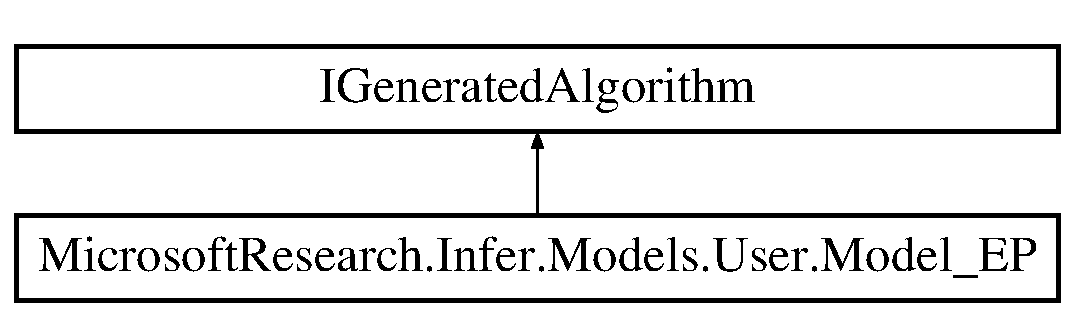
\includegraphics[height=2.000000cm]{class_microsoft_research_1_1_infer_1_1_models_1_1_user_1_1_model___e_p}
\end{center}
\end{figure}
\subsection*{Public Member Functions}
\begin{DoxyCompactItemize}
\item 
object \hyperlink{class_microsoft_research_1_1_infer_1_1_models_1_1_user_1_1_model___e_p_ad41ad455ee9c75d9eb227088e3908237}{Get\+Observed\+Value} (string variable\+Name)
\begin{DoxyCompactList}\small\item\em Get the observed value of the specified variable.\end{DoxyCompactList}\item 
void \hyperlink{class_microsoft_research_1_1_infer_1_1_models_1_1_user_1_1_model___e_p_a1784d712f959b19cf9b6dd1fad20aa9e}{Set\+Observed\+Value} (string variable\+Name, object value)
\begin{DoxyCompactList}\small\item\em Set the observed value of the specified variable.\end{DoxyCompactList}\item 
object \hyperlink{class_microsoft_research_1_1_infer_1_1_models_1_1_user_1_1_model___e_p_ad7fa30acf60524bfba9c5fa41db1dc32}{Marginal} (string variable\+Name)
\begin{DoxyCompactList}\small\item\em Get the marginal distribution (computed up to this point) of a variable\end{DoxyCompactList}\item 
T \hyperlink{class_microsoft_research_1_1_infer_1_1_models_1_1_user_1_1_model___e_p_a83c754cda6fc44c9d11b4b1f6a67de91}{Marginal$<$ T $>$} (string variable\+Name)
\begin{DoxyCompactList}\small\item\em Get the marginal distribution (computed up to this point) of a variable, converted to type T\end{DoxyCompactList}\item 
object \hyperlink{class_microsoft_research_1_1_infer_1_1_models_1_1_user_1_1_model___e_p_aebb71d022bc194202b191a255d3647fd}{Marginal} (string variable\+Name, string query)
\begin{DoxyCompactList}\small\item\em Get the query-\/specific marginal distribution of a variable.\end{DoxyCompactList}\item 
T \hyperlink{class_microsoft_research_1_1_infer_1_1_models_1_1_user_1_1_model___e_p_a5db0c41c9cd8c0896fea19890bf0184d}{Marginal$<$ T $>$} (string variable\+Name, string query)
\begin{DoxyCompactList}\small\item\em Get the query-\/specific marginal distribution of a variable, converted to type T\end{DoxyCompactList}\item 
void \hyperlink{class_microsoft_research_1_1_infer_1_1_models_1_1_user_1_1_model___e_p_a0555bf326d664050cd8706fe1ad718c9}{Execute} (int number\+Of\+Iterations)
\begin{DoxyCompactList}\small\item\em Update all marginals, by iterating message-\/passing the given number of times\end{DoxyCompactList}\item 
void \hyperlink{class_microsoft_research_1_1_infer_1_1_models_1_1_user_1_1_model___e_p_a666059fedd70c6ebafb77b7ba98adc35}{Update} (int additional\+Iterations)
\begin{DoxyCompactList}\small\item\em Update all marginals, by iterating message-\/passing an additional number of times\end{DoxyCompactList}\item 
void \hyperlink{class_microsoft_research_1_1_infer_1_1_models_1_1_user_1_1_model___e_p_a9b5187d265d55326778d4ed5144dafc9}{Reset} ()
\begin{DoxyCompactList}\small\item\em Reset all messages to their initial values. Sets Number\+Of\+Iterations\+Done to 0.\end{DoxyCompactList}\item 
Bernoulli \hyperlink{class_microsoft_research_1_1_infer_1_1_models_1_1_user_1_1_model___e_p_a4ec19be7ea41aaa244b21163ede5ef74}{Vbool0\+Marginal} ()
\begin{DoxyCompactList}\small\item\em Returns the marginal distribution for \textquotesingle{}vbool0\textquotesingle{} given by the current state of the message passing algorithm. \end{DoxyCompactList}\item 
Dirichlet \hyperlink{class_microsoft_research_1_1_infer_1_1_models_1_1_user_1_1_model___e_p_a952c766daae4076480acb780851fb3ad}{Background\+Label\+Prob\+Marginal} ()
\begin{DoxyCompactList}\small\item\em Returns the marginal distribution for \textquotesingle{}Background\+Label\+Prob\textquotesingle{} given by the current state of the message passing algorithm. \end{DoxyCompactList}\item 
Distribution\+Ref\+Array$<$ Distribution\+Ref\+Array$<$ Dirichlet, Vector $>$, Vector\mbox{[}$\,$\mbox{]}$>$ \hyperlink{class_microsoft_research_1_1_infer_1_1_models_1_1_user_1_1_model___e_p_ad8f6e5dd24857fe3d8874e77702f49ae}{Confusion\+Matrix\+Marginal} ()
\begin{DoxyCompactList}\small\item\em Returns the marginal distribution for \textquotesingle{}Confusion\+Matrix\textquotesingle{} given by the current state of the message passing algorithm. \end{DoxyCompactList}\item 
Distribution\+Ref\+Array$<$ Discrete, int $>$ \hyperlink{class_microsoft_research_1_1_infer_1_1_models_1_1_user_1_1_model___e_p_a9f3842349f089d86043d607a831d4307}{Truth\+Marginal} ()
\begin{DoxyCompactList}\small\item\em Returns the marginal distribution for \textquotesingle{}Truth\textquotesingle{} given by the current state of the message passing algorithm. \end{DoxyCompactList}\item 
Distribution\+Ref\+Array$<$ Discrete, int $>$ \hyperlink{class_microsoft_research_1_1_infer_1_1_models_1_1_user_1_1_model___e_p_a100991a01a0141905e4cf5bbab98108e}{Truth\+Marginal\+Divided\+By\+Prior} ()
\begin{DoxyCompactList}\small\item\em Returns the output message (the posterior divided by the prior) for \textquotesingle{}Truth\textquotesingle{} given by the current state of the message passing algorithm. \end{DoxyCompactList}\item 
Point\+Mass$<$ int $>$ \hyperlink{class_microsoft_research_1_1_infer_1_1_models_1_1_user_1_1_model___e_p_a03a6388334755ebd2aa0ff8c5ed1f4e2}{Worker\+Count\+Marginal} ()
\begin{DoxyCompactList}\small\item\em Returns the marginal distribution for \textquotesingle{}Worker\+Count\textquotesingle{} given by the current state of the message passing algorithm. \end{DoxyCompactList}\item 
Point\+Mass$<$ int\mbox{[}$\,$\mbox{]}$>$ \hyperlink{class_microsoft_research_1_1_infer_1_1_models_1_1_user_1_1_model___e_p_a94c95fb366462f663dc702374f1bea44}{Worker\+Task\+Count\+Marginal} ()
\begin{DoxyCompactList}\small\item\em Returns the marginal distribution for \textquotesingle{}Worker\+Task\+Count\textquotesingle{} given by the current state of the message passing algorithm. \end{DoxyCompactList}\item 
Point\+Mass$<$ int\mbox{[}$\,$\mbox{]}\mbox{[}$\,$\mbox{]}$>$ \hyperlink{class_microsoft_research_1_1_infer_1_1_models_1_1_user_1_1_model___e_p_a4010e430a8925a46d7a7098952773582}{Worker\+Task\+Index\+Marginal} ()
\begin{DoxyCompactList}\small\item\em Returns the marginal distribution for \textquotesingle{}Worker\+Task\+Index\textquotesingle{} given by the current state of the message passing algorithm. \end{DoxyCompactList}\item 
Point\+Mass$<$ Dirichlet $>$ \hyperlink{class_microsoft_research_1_1_infer_1_1_models_1_1_user_1_1_model___e_p_a217cb08f450040b58535d623bd7fa6b0}{Background\+Label\+Prob\+Prior\+Marginal} ()
\begin{DoxyCompactList}\small\item\em Returns the marginal distribution for \textquotesingle{}Background\+Label\+Prob\+Prior\textquotesingle{} given by the current state of the message passing algorithm. \end{DoxyCompactList}\item 
Point\+Mass$<$ Dirichlet\mbox{[}$\,$\mbox{]}\mbox{[}$\,$\mbox{]}$>$ \hyperlink{class_microsoft_research_1_1_infer_1_1_models_1_1_user_1_1_model___e_p_a31f2762b98ace26fd1659e251faf6379}{Confusion\+Matrix\+Prior\+Marginal} ()
\begin{DoxyCompactList}\small\item\em Returns the marginal distribution for \textquotesingle{}Confusion\+Matrix\+Prior\textquotesingle{} given by the current state of the message passing algorithm. \end{DoxyCompactList}\item 
Point\+Mass$<$ Discrete\mbox{[}$\,$\mbox{]}$>$ \hyperlink{class_microsoft_research_1_1_infer_1_1_models_1_1_user_1_1_model___e_p_a388fd0698994fcdf0afde5e07338fd6c}{Truth\+Constraint\+Marginal} ()
\begin{DoxyCompactList}\small\item\em Returns the marginal distribution for \textquotesingle{}Truth\+Constraint\textquotesingle{} given by the current state of the message passing algorithm. \end{DoxyCompactList}\item 
Distribution\+Ref\+Array$<$ Distribution\+Ref\+Array$<$ Discrete, int $>$, int\mbox{[}$\,$\mbox{]}$>$ \hyperlink{class_microsoft_research_1_1_infer_1_1_models_1_1_user_1_1_model___e_p_a8c09b2fe4a6625f7afd6b860187268af}{Worker\+Label\+Marginal} ()
\begin{DoxyCompactList}\small\item\em Returns the marginal distribution for \textquotesingle{}Worker\+Label\textquotesingle{} given by the current state of the message passing algorithm. \end{DoxyCompactList}\end{DoxyCompactItemize}
\subsection*{Public Attributes}
\begin{DoxyCompactItemize}
\item 
int \hyperlink{class_microsoft_research_1_1_infer_1_1_models_1_1_user_1_1_model___e_p_a68cc9b27a065511a79d56f87983fc56d}{Changed\+\_\+\+Worker\+Count\+\_\+\+Worker\+Task\+Count\+\_\+\+Worker\+Task\+Index\+\_\+\+Background\+Label\+Prob\+Prior\+\_\+\+Confusion\+Matrix\+Prior\+\_\+\+Tr0\+\_\+iterations\+Done}
\begin{DoxyCompactList}\small\item\em The number of iterations last computed by Changed\+\_\+\+Worker\+Count\+\_\+\+Worker\+Task\+Count\+\_\+\+Worker\+Task\+Index\+\_\+\+Background\+Label\+Prob\+Prior\+\_\+\+Confusion\+Matrix\+Prior\+\_\+\+Tr0. Set this to zero to force re-\/execution of Changed\+\_\+\+Worker\+Count\+\_\+\+Worker\+Task\+Count\+\_\+\+Worker\+Task\+Index\+\_\+\+Background\+Label\+Prob\+Prior\+\_\+\+Confusion\+Matrix\+Prior\+\_\+\+Tr0\end{DoxyCompactList}\item 
int \hyperlink{class_microsoft_research_1_1_infer_1_1_models_1_1_user_1_1_model___e_p_a6ba5341acb834c6b1b7afc6f339bc210}{Changed\+\_\+number\+Of\+Iterations\+Decreased\+\_\+\+Worker\+Count\+\_\+\+Confusion\+Matrix\+Prior\+\_\+\+Worker\+Task\+Count\+\_\+\+Worker\+Label\+\_\+\+Wor1\+\_\+iterations\+Done}
\begin{DoxyCompactList}\small\item\em The number of iterations last computed by Changed\+\_\+number\+Of\+Iterations\+Decreased\+\_\+\+Worker\+Count\+\_\+\+Confusion\+Matrix\+Prior\+\_\+\+Worker\+Task\+Count\+\_\+\+Worker\+Label\+\_\+\+Wor1. Set this to zero to force re-\/execution of Changed\+\_\+number\+Of\+Iterations\+Decreased\+\_\+\+Worker\+Count\+\_\+\+Confusion\+Matrix\+Prior\+\_\+\+Worker\+Task\+Count\+\_\+\+Worker\+Label\+\_\+\+Wor1\end{DoxyCompactList}\item 
int \hyperlink{class_microsoft_research_1_1_infer_1_1_models_1_1_user_1_1_model___e_p_a6dba112878fc8583d1a25218cb7da60d}{Changed\+\_\+\+Worker\+Count\+\_\+iterations\+Done}
\begin{DoxyCompactList}\small\item\em The number of iterations last computed by Changed\+\_\+\+Worker\+Count. Set this to zero to force re-\/execution of Changed\+\_\+\+Worker\+Count\end{DoxyCompactList}\item 
int \hyperlink{class_microsoft_research_1_1_infer_1_1_models_1_1_user_1_1_model___e_p_aa1a7d6b28fd11a566a03df6b6c06ddcb}{Changed\+\_\+\+Worker\+Count\+\_\+\+Worker\+Task\+Count\+\_\+iterations\+Done}
\begin{DoxyCompactList}\small\item\em The number of iterations last computed by Changed\+\_\+\+Worker\+Count\+\_\+\+Worker\+Task\+Count. Set this to zero to force re-\/execution of Changed\+\_\+\+Worker\+Count\+\_\+\+Worker\+Task\+Count\end{DoxyCompactList}\item 
int \hyperlink{class_microsoft_research_1_1_infer_1_1_models_1_1_user_1_1_model___e_p_a5bf8aef1624310fee144a221a1108716}{Changed\+\_\+\+Worker\+Count\+\_\+\+Worker\+Task\+Count\+\_\+\+Confusion\+Matrix\+Prior\+\_\+\+Init\+\_\+number\+Of\+Iterations\+Decreased\+\_\+\+Worker\+Labe4\+\_\+iterations\+Done}
\begin{DoxyCompactList}\small\item\em The number of iterations last computed by Changed\+\_\+\+Worker\+Count\+\_\+\+Worker\+Task\+Count\+\_\+\+Confusion\+Matrix\+Prior\+\_\+\+Init\+\_\+number\+Of\+Iterations\+Decreased\+\_\+\+Worker\+Labe4. Set this to zero to force re-\/execution of Changed\+\_\+\+Worker\+Count\+\_\+\+Worker\+Task\+Count\+\_\+\+Confusion\+Matrix\+Prior\+\_\+\+Init\+\_\+number\+Of\+Iterations\+Decreased\+\_\+\+Worker\+Labe4\end{DoxyCompactList}\item 
bool \hyperlink{class_microsoft_research_1_1_infer_1_1_models_1_1_user_1_1_model___e_p_ae305ba92155c72ca215b3948d87dd321}{Changed\+\_\+\+Worker\+Count\+\_\+\+Worker\+Task\+Count\+\_\+\+Confusion\+Matrix\+Prior\+\_\+\+Init\+\_\+number\+Of\+Iterations\+Decreased\+\_\+\+Worker\+Labe4\+\_\+is\+Initialised}
\begin{DoxyCompactList}\small\item\em True if Changed\+\_\+\+Worker\+Count\+\_\+\+Worker\+Task\+Count\+\_\+\+Confusion\+Matrix\+Prior\+\_\+\+Init\+\_\+number\+Of\+Iterations\+Decreased\+\_\+\+Worker\+Labe4 has performed initialisation. Set this to false to force re-\/execution of Changed\+\_\+\+Worker\+Count\+\_\+\+Worker\+Task\+Count\+\_\+\+Confusion\+Matrix\+Prior\+\_\+\+Init\+\_\+number\+Of\+Iterations\+Decreased\+\_\+\+Worker\+Labe4\end{DoxyCompactList}\item 
int \hyperlink{class_microsoft_research_1_1_infer_1_1_models_1_1_user_1_1_model___e_p_a90f97411af644a567896bd38068a3681}{Changed\+\_\+\+Worker\+Count\+\_\+\+Confusion\+Matrix\+Prior\+\_\+\+Init\+\_\+number\+Of\+Iterations\+Decreased\+\_\+\+Worker\+Task\+Count\+\_\+\+Worker\+Labe5\+\_\+iterations\+Done}
\begin{DoxyCompactList}\small\item\em The number of iterations last computed by Changed\+\_\+\+Worker\+Count\+\_\+\+Confusion\+Matrix\+Prior\+\_\+\+Init\+\_\+number\+Of\+Iterations\+Decreased\+\_\+\+Worker\+Task\+Count\+\_\+\+Worker\+Labe5. Set this to zero to force re-\/execution of Changed\+\_\+\+Worker\+Count\+\_\+\+Confusion\+Matrix\+Prior\+\_\+\+Init\+\_\+number\+Of\+Iterations\+Decreased\+\_\+\+Worker\+Task\+Count\+\_\+\+Worker\+Labe5\end{DoxyCompactList}\item 
bool \hyperlink{class_microsoft_research_1_1_infer_1_1_models_1_1_user_1_1_model___e_p_abad013c605a772f90c9b7c700fcfe077}{Changed\+\_\+\+Worker\+Count\+\_\+\+Confusion\+Matrix\+Prior\+\_\+\+Init\+\_\+number\+Of\+Iterations\+Decreased\+\_\+\+Worker\+Task\+Count\+\_\+\+Worker\+Labe5\+\_\+is\+Initialised}
\begin{DoxyCompactList}\small\item\em True if Changed\+\_\+\+Worker\+Count\+\_\+\+Confusion\+Matrix\+Prior\+\_\+\+Init\+\_\+number\+Of\+Iterations\+Decreased\+\_\+\+Worker\+Task\+Count\+\_\+\+Worker\+Labe5 has performed initialisation. Set this to false to force re-\/execution of Changed\+\_\+\+Worker\+Count\+\_\+\+Confusion\+Matrix\+Prior\+\_\+\+Init\+\_\+number\+Of\+Iterations\+Decreased\+\_\+\+Worker\+Task\+Count\+\_\+\+Worker\+Labe5\end{DoxyCompactList}\item 
int \hyperlink{class_microsoft_research_1_1_infer_1_1_models_1_1_user_1_1_model___e_p_a96cd83a67ce48692b2dd5f13b31f06b9}{Constant\+\_\+iterations\+Done}
\begin{DoxyCompactList}\small\item\em The number of iterations last computed by Constant. Set this to zero to force re-\/execution of Constant\end{DoxyCompactList}\item 
int \hyperlink{class_microsoft_research_1_1_infer_1_1_models_1_1_user_1_1_model___e_p_ae58eb5265f8700b885d370e8fe410802}{Changed\+\_\+\+Background\+Label\+Prob\+Prior\+\_\+\+Init\+\_\+number\+Of\+Iterations\+Decreased\+\_\+\+Worker\+Count\+\_\+\+Confusion\+Matrix\+Prior\+\_\+\+W7\+\_\+iterations\+Done}
\begin{DoxyCompactList}\small\item\em The number of iterations last computed by Changed\+\_\+\+Background\+Label\+Prob\+Prior\+\_\+\+Init\+\_\+number\+Of\+Iterations\+Decreased\+\_\+\+Worker\+Count\+\_\+\+Confusion\+Matrix\+Prior\+\_\+\+W7. Set this to zero to force re-\/execution of Changed\+\_\+\+Background\+Label\+Prob\+Prior\+\_\+\+Init\+\_\+number\+Of\+Iterations\+Decreased\+\_\+\+Worker\+Count\+\_\+\+Confusion\+Matrix\+Prior\+\_\+\+W7\end{DoxyCompactList}\item 
bool \hyperlink{class_microsoft_research_1_1_infer_1_1_models_1_1_user_1_1_model___e_p_a2e04d5d41ac542942b2b715e26bd4038}{Changed\+\_\+\+Background\+Label\+Prob\+Prior\+\_\+\+Init\+\_\+number\+Of\+Iterations\+Decreased\+\_\+\+Worker\+Count\+\_\+\+Confusion\+Matrix\+Prior\+\_\+\+W7\+\_\+is\+Initialised}
\begin{DoxyCompactList}\small\item\em True if Changed\+\_\+\+Background\+Label\+Prob\+Prior\+\_\+\+Init\+\_\+number\+Of\+Iterations\+Decreased\+\_\+\+Worker\+Count\+\_\+\+Confusion\+Matrix\+Prior\+\_\+\+W7 has performed initialisation. Set this to false to force re-\/execution of Changed\+\_\+\+Background\+Label\+Prob\+Prior\+\_\+\+Init\+\_\+number\+Of\+Iterations\+Decreased\+\_\+\+Worker\+Count\+\_\+\+Confusion\+Matrix\+Prior\+\_\+\+W7\end{DoxyCompactList}\item 
\hypertarget{class_microsoft_research_1_1_infer_1_1_models_1_1_user_1_1_model___e_p_aae95c2a5d450ae29e8296fef01dd762c}{}Distribution\+Ref\+Array$<$ Dirichlet, Vector $>$ {\bfseries Background\+Label\+Prob\+\_\+rep\+\_\+\+B}\label{class_microsoft_research_1_1_infer_1_1_models_1_1_user_1_1_model___e_p_aae95c2a5d450ae29e8296fef01dd762c}

\item 
Dirichlet \hyperlink{class_microsoft_research_1_1_infer_1_1_models_1_1_user_1_1_model___e_p_ada4c5df5755a4a5d434327e99fc0e52e}{Background\+Label\+Prob\+\_\+rep\+\_\+\+F\+\_\+marginal}
\begin{DoxyCompactList}\small\item\em Buffer for Replicate\+Op\+\_\+\+Divide.\+Uses\+Average\+Conditional$<$\+Dirichlet$>$\end{DoxyCompactList}\item 
\hypertarget{class_microsoft_research_1_1_infer_1_1_models_1_1_user_1_1_model___e_p_a23af40d289a65eda2de8c88cbbec3ff5}{}Distribution\+Ref\+Array$<$ Distribution\+Ref\+Array$<$ Distribution\+Ref\+Array$<$ Dirichlet, Vector $>$, Vector\mbox{[}$\,$\mbox{]}$>$, Vector\mbox{[}$\,$\mbox{]}\mbox{[}$\,$\mbox{]}$>$ {\bfseries Confusion\+Matrix\+\_\+rep\+\_\+\+B}\label{class_microsoft_research_1_1_infer_1_1_models_1_1_user_1_1_model___e_p_a23af40d289a65eda2de8c88cbbec3ff5}

\item 
Distribution\+Ref\+Array$<$ Distribution\+Ref\+Array$<$ Dirichlet, Vector $>$, Vector\mbox{[}$\,$\mbox{]}$>$ \hyperlink{class_microsoft_research_1_1_infer_1_1_models_1_1_user_1_1_model___e_p_a3590fbf0f60f036123242d4f0baa5c4f}{Confusion\+Matrix\+\_\+rep\+\_\+\+B\+\_\+to\+Def}
\begin{DoxyCompactList}\small\item\em Buffer for Replicate\+Op\+\_\+\+Divide.\+Marginal$<$\+Dirichlet$>$\end{DoxyCompactList}\item 
Distribution\+Ref\+Array$<$ Discrete, int $>$ \hyperlink{class_microsoft_research_1_1_infer_1_1_models_1_1_user_1_1_model___e_p_ac3fc54a4524ee40acdab6aad09631bc7}{Truth\+\_\+uses\+\_\+\+B\+\_\+n\+\_\+\+\_\+to\+Def}
\begin{DoxyCompactList}\small\item\em Buffer for Replicate\+Op\+\_\+\+Divide.\+Marginal$<$\+Discrete$>$\end{DoxyCompactList}\item 
Bernoulli \hyperlink{class_microsoft_research_1_1_infer_1_1_models_1_1_user_1_1_model___e_p_ac90e3796c29c3bbcb0ad85d8e8ac90c2}{vbool0\+\_\+marginal\+\_\+\+F}
\begin{DoxyCompactList}\small\item\em Message to marginal of \textquotesingle{}vbool0\textquotesingle{}\end{DoxyCompactList}\item 
Dirichlet \hyperlink{class_microsoft_research_1_1_infer_1_1_models_1_1_user_1_1_model___e_p_ad123c1c17c747bf809749496b903795e}{Background\+Label\+Prob\+\_\+marginal\+\_\+\+F}
\begin{DoxyCompactList}\small\item\em Message to marginal of \textquotesingle{}Background\+Label\+Prob\textquotesingle{}\end{DoxyCompactList}\item 
Distribution\+Ref\+Array$<$ Distribution\+Ref\+Array$<$ Dirichlet, Vector $>$, Vector\mbox{[}$\,$\mbox{]}$>$ \hyperlink{class_microsoft_research_1_1_infer_1_1_models_1_1_user_1_1_model___e_p_a826248ad56421c86f0f047e958f5fbce}{Confusion\+Matrix\+\_\+marginal\+\_\+\+F}
\begin{DoxyCompactList}\small\item\em Message to marginal of \textquotesingle{}Confusion\+Matrix\textquotesingle{}\end{DoxyCompactList}\item 
Distribution\+Ref\+Array$<$ Discrete, int $>$ \hyperlink{class_microsoft_research_1_1_infer_1_1_models_1_1_user_1_1_model___e_p_ac0f71b3998592b33f9b4025f39d97a40}{Truth\+\_\+marginal\+\_\+\+F}
\begin{DoxyCompactList}\small\item\em Message to marginal of \textquotesingle{}Truth\textquotesingle{}\end{DoxyCompactList}\item 
\hypertarget{class_microsoft_research_1_1_infer_1_1_models_1_1_user_1_1_model___e_p_ac05ae9eb4c7d49051bba627421994ad6}{}Point\+Mass$<$ int $>$ {\bfseries Worker\+Count\+\_\+marginal}\label{class_microsoft_research_1_1_infer_1_1_models_1_1_user_1_1_model___e_p_ac05ae9eb4c7d49051bba627421994ad6}

\item 
\hypertarget{class_microsoft_research_1_1_infer_1_1_models_1_1_user_1_1_model___e_p_ac236fcc7606e7135faf98300bdda2840}{}Point\+Mass$<$ int\mbox{[}$\,$\mbox{]}$>$ {\bfseries Worker\+Task\+Count\+\_\+marginal}\label{class_microsoft_research_1_1_infer_1_1_models_1_1_user_1_1_model___e_p_ac236fcc7606e7135faf98300bdda2840}

\item 
\hypertarget{class_microsoft_research_1_1_infer_1_1_models_1_1_user_1_1_model___e_p_abac4131c53e234262731e0a07c3852e6}{}Point\+Mass$<$ int\mbox{[}$\,$\mbox{]}\mbox{[}$\,$\mbox{]}$>$ {\bfseries Worker\+Task\+Index\+\_\+marginal}\label{class_microsoft_research_1_1_infer_1_1_models_1_1_user_1_1_model___e_p_abac4131c53e234262731e0a07c3852e6}

\item 
\hypertarget{class_microsoft_research_1_1_infer_1_1_models_1_1_user_1_1_model___e_p_a111766b07f18f7783077a68d3b1c989f}{}Point\+Mass$<$ Dirichlet $>$ {\bfseries Background\+Label\+Prob\+Prior\+\_\+marginal}\label{class_microsoft_research_1_1_infer_1_1_models_1_1_user_1_1_model___e_p_a111766b07f18f7783077a68d3b1c989f}

\item 
\hypertarget{class_microsoft_research_1_1_infer_1_1_models_1_1_user_1_1_model___e_p_a03edc2556c23997e63776a990ec4a6c2}{}Point\+Mass$<$ Dirichlet\mbox{[}$\,$\mbox{]}\mbox{[}$\,$\mbox{]}$>$ {\bfseries Confusion\+Matrix\+Prior\+\_\+marginal}\label{class_microsoft_research_1_1_infer_1_1_models_1_1_user_1_1_model___e_p_a03edc2556c23997e63776a990ec4a6c2}

\item 
\hypertarget{class_microsoft_research_1_1_infer_1_1_models_1_1_user_1_1_model___e_p_a3745e965cabc6957ea9eecfcd4015df5}{}Point\+Mass$<$ Discrete\mbox{[}$\,$\mbox{]}$>$ {\bfseries Truth\+Constraint\+\_\+marginal}\label{class_microsoft_research_1_1_infer_1_1_models_1_1_user_1_1_model___e_p_a3745e965cabc6957ea9eecfcd4015df5}

\item 
\hypertarget{class_microsoft_research_1_1_infer_1_1_models_1_1_user_1_1_model___e_p_a8e3e8801f3d7aa01655a3ec06aaeb4b4}{}Distribution\+Ref\+Array$<$ Distribution\+Ref\+Array$<$ Discrete, int $>$, int\mbox{[}$\,$\mbox{]}$>$ {\bfseries Worker\+Label\+\_\+marginal}\label{class_microsoft_research_1_1_infer_1_1_models_1_1_user_1_1_model___e_p_a8e3e8801f3d7aa01655a3ec06aaeb4b4}

\end{DoxyCompactItemize}
\subsection*{Properties}
\begin{DoxyCompactItemize}
\item 
int \hyperlink{class_microsoft_research_1_1_infer_1_1_models_1_1_user_1_1_model___e_p_a0a9e34e70ccab7709f1134b9b5889a47}{Number\+Of\+Iterations\+Done}\hspace{0.3cm}{\ttfamily  \mbox{[}get\mbox{]}}
\begin{DoxyCompactList}\small\item\em The number of iterations done from the initial state\end{DoxyCompactList}\item 
int \hyperlink{class_microsoft_research_1_1_infer_1_1_models_1_1_user_1_1_model___e_p_a918e710a2e7b4a123da74eced7421ece}{Worker\+Count}\hspace{0.3cm}{\ttfamily  \mbox{[}get, set\mbox{]}}
\begin{DoxyCompactList}\small\item\em The externally-\/specified value of \textquotesingle{}Worker\+Count\textquotesingle{}\end{DoxyCompactList}\item 
int\mbox{[}$\,$\mbox{]} \hyperlink{class_microsoft_research_1_1_infer_1_1_models_1_1_user_1_1_model___e_p_adba9d5853dd6a6ab74401c6c4316d348}{Worker\+Task\+Count}\hspace{0.3cm}{\ttfamily  \mbox{[}get, set\mbox{]}}
\begin{DoxyCompactList}\small\item\em The externally-\/specified value of \textquotesingle{}Worker\+Task\+Count\textquotesingle{}\end{DoxyCompactList}\item 
int\mbox{[}$\,$\mbox{]}\mbox{[}$\,$\mbox{]} \hyperlink{class_microsoft_research_1_1_infer_1_1_models_1_1_user_1_1_model___e_p_acabd7291b2d88f17a2df55a702f71e29}{Worker\+Task\+Index}\hspace{0.3cm}{\ttfamily  \mbox{[}get, set\mbox{]}}
\begin{DoxyCompactList}\small\item\em The externally-\/specified value of \textquotesingle{}Worker\+Task\+Index\textquotesingle{}\end{DoxyCompactList}\item 
Dirichlet \hyperlink{class_microsoft_research_1_1_infer_1_1_models_1_1_user_1_1_model___e_p_a5e94a159f468e8d365321779a4ac8ea1}{Background\+Label\+Prob\+Prior}\hspace{0.3cm}{\ttfamily  \mbox{[}get, set\mbox{]}}
\begin{DoxyCompactList}\small\item\em The externally-\/specified value of \textquotesingle{}Background\+Label\+Prob\+Prior\textquotesingle{}\end{DoxyCompactList}\item 
Dirichlet\mbox{[}$\,$\mbox{]}\mbox{[}$\,$\mbox{]} \hyperlink{class_microsoft_research_1_1_infer_1_1_models_1_1_user_1_1_model___e_p_a5d2f1483d0debe876c9c9504738761e7}{Confusion\+Matrix\+Prior}\hspace{0.3cm}{\ttfamily  \mbox{[}get, set\mbox{]}}
\begin{DoxyCompactList}\small\item\em The externally-\/specified value of \textquotesingle{}Confusion\+Matrix\+Prior\textquotesingle{}\end{DoxyCompactList}\item 
Discrete\mbox{[}$\,$\mbox{]} \hyperlink{class_microsoft_research_1_1_infer_1_1_models_1_1_user_1_1_model___e_p_acffd4167727f940a144a3efadfc2d805}{Truth\+Constraint}\hspace{0.3cm}{\ttfamily  \mbox{[}get, set\mbox{]}}
\begin{DoxyCompactList}\small\item\em The externally-\/specified value of \textquotesingle{}Truth\+Constraint\textquotesingle{}\end{DoxyCompactList}\item 
int\mbox{[}$\,$\mbox{]}\mbox{[}$\,$\mbox{]} \hyperlink{class_microsoft_research_1_1_infer_1_1_models_1_1_user_1_1_model___e_p_a719f0824f1c1f497c4c4e29e61125b67}{Worker\+Label}\hspace{0.3cm}{\ttfamily  \mbox{[}get, set\mbox{]}}
\begin{DoxyCompactList}\small\item\em The externally-\/specified value of \textquotesingle{}Worker\+Label\textquotesingle{}\end{DoxyCompactList}\end{DoxyCompactItemize}
\subsection*{Events}
\begin{DoxyCompactItemize}
\item 
Event\+Handler$<$ Progress\+Changed\+Event\+Args $>$ \hyperlink{class_microsoft_research_1_1_infer_1_1_models_1_1_user_1_1_model___e_p_ae3a4699a135334bb8924925ab33a1999}{Progress\+Changed}
\begin{DoxyCompactList}\small\item\em Event that is fired when the progress of inference changes, typically at the end of one iteration of the inference algorithm.\end{DoxyCompactList}\end{DoxyCompactItemize}


\subsection{Detailed Description}
Generated algorithm for performing inference. 

If you wish to use this class directly, you must perform the following steps\+: 1) Create an instance of the class. 2) Set the value of any externally-\/set fields e.\+g. data, priors. 3) Call the Execute(number\+Of\+Iterations) method. 4) Use the X\+X\+X\+Marginal() methods to retrieve posterior marginals for different variables.

Generated by Infer.\+N\+E\+T 2.\+6.\+41114.\+1 at 21\+:00 on 21 April 2015. 

\subsection{Member Function Documentation}
\hypertarget{class_microsoft_research_1_1_infer_1_1_models_1_1_user_1_1_model___e_p_a952c766daae4076480acb780851fb3ad}{}\index{Microsoft\+Research\+::\+Infer\+::\+Models\+::\+User\+::\+Model\+\_\+\+E\+P@{Microsoft\+Research\+::\+Infer\+::\+Models\+::\+User\+::\+Model\+\_\+\+E\+P}!Background\+Label\+Prob\+Marginal@{Background\+Label\+Prob\+Marginal}}
\index{Background\+Label\+Prob\+Marginal@{Background\+Label\+Prob\+Marginal}!Microsoft\+Research\+::\+Infer\+::\+Models\+::\+User\+::\+Model\+\_\+\+E\+P@{Microsoft\+Research\+::\+Infer\+::\+Models\+::\+User\+::\+Model\+\_\+\+E\+P}}
\subsubsection[{Background\+Label\+Prob\+Marginal()}]{\setlength{\rightskip}{0pt plus 5cm}Dirichlet Microsoft\+Research.\+Infer.\+Models.\+User.\+Model\+\_\+\+E\+P.\+Background\+Label\+Prob\+Marginal (
\begin{DoxyParamCaption}
{}
\end{DoxyParamCaption}
)\hspace{0.3cm}{\ttfamily [inline]}}\label{class_microsoft_research_1_1_infer_1_1_models_1_1_user_1_1_model___e_p_a952c766daae4076480acb780851fb3ad}


Returns the marginal distribution for \textquotesingle{}Background\+Label\+Prob\textquotesingle{} given by the current state of the message passing algorithm. 

\begin{DoxyReturn}{Returns}
The marginal distribution
\end{DoxyReturn}
\hypertarget{class_microsoft_research_1_1_infer_1_1_models_1_1_user_1_1_model___e_p_a217cb08f450040b58535d623bd7fa6b0}{}\index{Microsoft\+Research\+::\+Infer\+::\+Models\+::\+User\+::\+Model\+\_\+\+E\+P@{Microsoft\+Research\+::\+Infer\+::\+Models\+::\+User\+::\+Model\+\_\+\+E\+P}!Background\+Label\+Prob\+Prior\+Marginal@{Background\+Label\+Prob\+Prior\+Marginal}}
\index{Background\+Label\+Prob\+Prior\+Marginal@{Background\+Label\+Prob\+Prior\+Marginal}!Microsoft\+Research\+::\+Infer\+::\+Models\+::\+User\+::\+Model\+\_\+\+E\+P@{Microsoft\+Research\+::\+Infer\+::\+Models\+::\+User\+::\+Model\+\_\+\+E\+P}}
\subsubsection[{Background\+Label\+Prob\+Prior\+Marginal()}]{\setlength{\rightskip}{0pt plus 5cm}Point\+Mass$<$Dirichlet$>$ Microsoft\+Research.\+Infer.\+Models.\+User.\+Model\+\_\+\+E\+P.\+Background\+Label\+Prob\+Prior\+Marginal (
\begin{DoxyParamCaption}
{}
\end{DoxyParamCaption}
)\hspace{0.3cm}{\ttfamily [inline]}}\label{class_microsoft_research_1_1_infer_1_1_models_1_1_user_1_1_model___e_p_a217cb08f450040b58535d623bd7fa6b0}


Returns the marginal distribution for \textquotesingle{}Background\+Label\+Prob\+Prior\textquotesingle{} given by the current state of the message passing algorithm. 

\begin{DoxyReturn}{Returns}
The marginal distribution
\end{DoxyReturn}
\hypertarget{class_microsoft_research_1_1_infer_1_1_models_1_1_user_1_1_model___e_p_ad8f6e5dd24857fe3d8874e77702f49ae}{}\index{Microsoft\+Research\+::\+Infer\+::\+Models\+::\+User\+::\+Model\+\_\+\+E\+P@{Microsoft\+Research\+::\+Infer\+::\+Models\+::\+User\+::\+Model\+\_\+\+E\+P}!Confusion\+Matrix\+Marginal@{Confusion\+Matrix\+Marginal}}
\index{Confusion\+Matrix\+Marginal@{Confusion\+Matrix\+Marginal}!Microsoft\+Research\+::\+Infer\+::\+Models\+::\+User\+::\+Model\+\_\+\+E\+P@{Microsoft\+Research\+::\+Infer\+::\+Models\+::\+User\+::\+Model\+\_\+\+E\+P}}
\subsubsection[{Confusion\+Matrix\+Marginal()}]{\setlength{\rightskip}{0pt plus 5cm}Distribution\+Ref\+Array$<$Distribution\+Ref\+Array$<$Dirichlet,Vector$>$,Vector\mbox{[}$\,$\mbox{]}$>$ Microsoft\+Research.\+Infer.\+Models.\+User.\+Model\+\_\+\+E\+P.\+Confusion\+Matrix\+Marginal (
\begin{DoxyParamCaption}
{}
\end{DoxyParamCaption}
)\hspace{0.3cm}{\ttfamily [inline]}}\label{class_microsoft_research_1_1_infer_1_1_models_1_1_user_1_1_model___e_p_ad8f6e5dd24857fe3d8874e77702f49ae}


Returns the marginal distribution for \textquotesingle{}Confusion\+Matrix\textquotesingle{} given by the current state of the message passing algorithm. 

\begin{DoxyReturn}{Returns}
The marginal distribution
\end{DoxyReturn}
\hypertarget{class_microsoft_research_1_1_infer_1_1_models_1_1_user_1_1_model___e_p_a31f2762b98ace26fd1659e251faf6379}{}\index{Microsoft\+Research\+::\+Infer\+::\+Models\+::\+User\+::\+Model\+\_\+\+E\+P@{Microsoft\+Research\+::\+Infer\+::\+Models\+::\+User\+::\+Model\+\_\+\+E\+P}!Confusion\+Matrix\+Prior\+Marginal@{Confusion\+Matrix\+Prior\+Marginal}}
\index{Confusion\+Matrix\+Prior\+Marginal@{Confusion\+Matrix\+Prior\+Marginal}!Microsoft\+Research\+::\+Infer\+::\+Models\+::\+User\+::\+Model\+\_\+\+E\+P@{Microsoft\+Research\+::\+Infer\+::\+Models\+::\+User\+::\+Model\+\_\+\+E\+P}}
\subsubsection[{Confusion\+Matrix\+Prior\+Marginal()}]{\setlength{\rightskip}{0pt plus 5cm}Point\+Mass$<$Dirichlet\mbox{[}$\,$\mbox{]}\mbox{[}$\,$\mbox{]}$>$ Microsoft\+Research.\+Infer.\+Models.\+User.\+Model\+\_\+\+E\+P.\+Confusion\+Matrix\+Prior\+Marginal (
\begin{DoxyParamCaption}
{}
\end{DoxyParamCaption}
)\hspace{0.3cm}{\ttfamily [inline]}}\label{class_microsoft_research_1_1_infer_1_1_models_1_1_user_1_1_model___e_p_a31f2762b98ace26fd1659e251faf6379}


Returns the marginal distribution for \textquotesingle{}Confusion\+Matrix\+Prior\textquotesingle{} given by the current state of the message passing algorithm. 

\begin{DoxyReturn}{Returns}
The marginal distribution
\end{DoxyReturn}
\hypertarget{class_microsoft_research_1_1_infer_1_1_models_1_1_user_1_1_model___e_p_a0555bf326d664050cd8706fe1ad718c9}{}\index{Microsoft\+Research\+::\+Infer\+::\+Models\+::\+User\+::\+Model\+\_\+\+E\+P@{Microsoft\+Research\+::\+Infer\+::\+Models\+::\+User\+::\+Model\+\_\+\+E\+P}!Execute@{Execute}}
\index{Execute@{Execute}!Microsoft\+Research\+::\+Infer\+::\+Models\+::\+User\+::\+Model\+\_\+\+E\+P@{Microsoft\+Research\+::\+Infer\+::\+Models\+::\+User\+::\+Model\+\_\+\+E\+P}}
\subsubsection[{Execute(int number\+Of\+Iterations)}]{\setlength{\rightskip}{0pt plus 5cm}void Microsoft\+Research.\+Infer.\+Models.\+User.\+Model\+\_\+\+E\+P.\+Execute (
\begin{DoxyParamCaption}
\item[{int}]{number\+Of\+Iterations}
\end{DoxyParamCaption}
)\hspace{0.3cm}{\ttfamily [inline]}}\label{class_microsoft_research_1_1_infer_1_1_models_1_1_user_1_1_model___e_p_a0555bf326d664050cd8706fe1ad718c9}


Update all marginals, by iterating message-\/passing the given number of times


\begin{DoxyParams}{Parameters}
{\em number\+Of\+Iterations} & The total number of iterations that should be executed for the current set of observed values. If this is more than the number already done, only the extra iterations are done. If this is less than the number already done, message-\/passing is restarted from the beginning. Changing the observed values resets the iteration count to 0.\\
\hline
\end{DoxyParams}
\hypertarget{class_microsoft_research_1_1_infer_1_1_models_1_1_user_1_1_model___e_p_ad41ad455ee9c75d9eb227088e3908237}{}\index{Microsoft\+Research\+::\+Infer\+::\+Models\+::\+User\+::\+Model\+\_\+\+E\+P@{Microsoft\+Research\+::\+Infer\+::\+Models\+::\+User\+::\+Model\+\_\+\+E\+P}!Get\+Observed\+Value@{Get\+Observed\+Value}}
\index{Get\+Observed\+Value@{Get\+Observed\+Value}!Microsoft\+Research\+::\+Infer\+::\+Models\+::\+User\+::\+Model\+\_\+\+E\+P@{Microsoft\+Research\+::\+Infer\+::\+Models\+::\+User\+::\+Model\+\_\+\+E\+P}}
\subsubsection[{Get\+Observed\+Value(string variable\+Name)}]{\setlength{\rightskip}{0pt plus 5cm}object Microsoft\+Research.\+Infer.\+Models.\+User.\+Model\+\_\+\+E\+P.\+Get\+Observed\+Value (
\begin{DoxyParamCaption}
\item[{string}]{variable\+Name}
\end{DoxyParamCaption}
)\hspace{0.3cm}{\ttfamily [inline]}}\label{class_microsoft_research_1_1_infer_1_1_models_1_1_user_1_1_model___e_p_ad41ad455ee9c75d9eb227088e3908237}


Get the observed value of the specified variable.


\begin{DoxyParams}{Parameters}
{\em variable\+Name} & Variable name\\
\hline
\end{DoxyParams}
\hypertarget{class_microsoft_research_1_1_infer_1_1_models_1_1_user_1_1_model___e_p_ad7fa30acf60524bfba9c5fa41db1dc32}{}\index{Microsoft\+Research\+::\+Infer\+::\+Models\+::\+User\+::\+Model\+\_\+\+E\+P@{Microsoft\+Research\+::\+Infer\+::\+Models\+::\+User\+::\+Model\+\_\+\+E\+P}!Marginal@{Marginal}}
\index{Marginal@{Marginal}!Microsoft\+Research\+::\+Infer\+::\+Models\+::\+User\+::\+Model\+\_\+\+E\+P@{Microsoft\+Research\+::\+Infer\+::\+Models\+::\+User\+::\+Model\+\_\+\+E\+P}}
\subsubsection[{Marginal(string variable\+Name)}]{\setlength{\rightskip}{0pt plus 5cm}object Microsoft\+Research.\+Infer.\+Models.\+User.\+Model\+\_\+\+E\+P.\+Marginal (
\begin{DoxyParamCaption}
\item[{string}]{variable\+Name}
\end{DoxyParamCaption}
)\hspace{0.3cm}{\ttfamily [inline]}}\label{class_microsoft_research_1_1_infer_1_1_models_1_1_user_1_1_model___e_p_ad7fa30acf60524bfba9c5fa41db1dc32}


Get the marginal distribution (computed up to this point) of a variable


\begin{DoxyParams}{Parameters}
{\em variable\+Name} & Name of the variable in the generated code\\
\hline
\end{DoxyParams}
\begin{DoxyReturn}{Returns}
The marginal distribution computed up to this point
\end{DoxyReturn}


Execute, Update, or Reset must be called first to set the value of the marginal.\hypertarget{class_microsoft_research_1_1_infer_1_1_models_1_1_user_1_1_model___e_p_aebb71d022bc194202b191a255d3647fd}{}\index{Microsoft\+Research\+::\+Infer\+::\+Models\+::\+User\+::\+Model\+\_\+\+E\+P@{Microsoft\+Research\+::\+Infer\+::\+Models\+::\+User\+::\+Model\+\_\+\+E\+P}!Marginal@{Marginal}}
\index{Marginal@{Marginal}!Microsoft\+Research\+::\+Infer\+::\+Models\+::\+User\+::\+Model\+\_\+\+E\+P@{Microsoft\+Research\+::\+Infer\+::\+Models\+::\+User\+::\+Model\+\_\+\+E\+P}}
\subsubsection[{Marginal(string variable\+Name, string query)}]{\setlength{\rightskip}{0pt plus 5cm}object Microsoft\+Research.\+Infer.\+Models.\+User.\+Model\+\_\+\+E\+P.\+Marginal (
\begin{DoxyParamCaption}
\item[{string}]{variable\+Name, }
\item[{string}]{query}
\end{DoxyParamCaption}
)\hspace{0.3cm}{\ttfamily [inline]}}\label{class_microsoft_research_1_1_infer_1_1_models_1_1_user_1_1_model___e_p_aebb71d022bc194202b191a255d3647fd}


Get the query-\/specific marginal distribution of a variable.


\begin{DoxyParams}{Parameters}
{\em variable\+Name} & Name of the variable in the generated code\\
\hline
{\em query} & Query\+Type name. For example, Gibbs\+Sampling answers \textquotesingle{}Marginal\textquotesingle{}, \textquotesingle{}Samples\textquotesingle{}, and \textquotesingle{}Conditionals\textquotesingle{} queries\\
\hline
\end{DoxyParams}


Execute, Update, or Reset must be called first to set the value of the marginal.\hypertarget{class_microsoft_research_1_1_infer_1_1_models_1_1_user_1_1_model___e_p_a83c754cda6fc44c9d11b4b1f6a67de91}{}\index{Microsoft\+Research\+::\+Infer\+::\+Models\+::\+User\+::\+Model\+\_\+\+E\+P@{Microsoft\+Research\+::\+Infer\+::\+Models\+::\+User\+::\+Model\+\_\+\+E\+P}!Marginal$<$ T $>$@{Marginal$<$ T $>$}}
\index{Marginal$<$ T $>$@{Marginal$<$ T $>$}!Microsoft\+Research\+::\+Infer\+::\+Models\+::\+User\+::\+Model\+\_\+\+E\+P@{Microsoft\+Research\+::\+Infer\+::\+Models\+::\+User\+::\+Model\+\_\+\+E\+P}}
\subsubsection[{Marginal$<$ T $>$(string variable\+Name)}]{\setlength{\rightskip}{0pt plus 5cm}T {\bf Microsoft\+Research.\+Infer.\+Models.\+User.\+Model\+\_\+\+E\+P.\+Marginal}$<$ T $>$ (
\begin{DoxyParamCaption}
\item[{string}]{variable\+Name}
\end{DoxyParamCaption}
)\hspace{0.3cm}{\ttfamily [inline]}}\label{class_microsoft_research_1_1_infer_1_1_models_1_1_user_1_1_model___e_p_a83c754cda6fc44c9d11b4b1f6a67de91}


Get the marginal distribution (computed up to this point) of a variable, converted to type T


\begin{DoxyTemplParams}{Template Parameters}
{\em T} & The distribution type.\\
\hline
\end{DoxyTemplParams}

\begin{DoxyParams}{Parameters}
{\em variable\+Name} & Name of the variable in the generated code\\
\hline
\end{DoxyParams}
\begin{DoxyReturn}{Returns}
The marginal distribution computed up to this point
\end{DoxyReturn}


Execute, Update, or Reset must be called first to set the value of the marginal.\hypertarget{class_microsoft_research_1_1_infer_1_1_models_1_1_user_1_1_model___e_p_a5db0c41c9cd8c0896fea19890bf0184d}{}\index{Microsoft\+Research\+::\+Infer\+::\+Models\+::\+User\+::\+Model\+\_\+\+E\+P@{Microsoft\+Research\+::\+Infer\+::\+Models\+::\+User\+::\+Model\+\_\+\+E\+P}!Marginal$<$ T $>$@{Marginal$<$ T $>$}}
\index{Marginal$<$ T $>$@{Marginal$<$ T $>$}!Microsoft\+Research\+::\+Infer\+::\+Models\+::\+User\+::\+Model\+\_\+\+E\+P@{Microsoft\+Research\+::\+Infer\+::\+Models\+::\+User\+::\+Model\+\_\+\+E\+P}}
\subsubsection[{Marginal$<$ T $>$(string variable\+Name, string query)}]{\setlength{\rightskip}{0pt plus 5cm}T {\bf Microsoft\+Research.\+Infer.\+Models.\+User.\+Model\+\_\+\+E\+P.\+Marginal}$<$ T $>$ (
\begin{DoxyParamCaption}
\item[{string}]{variable\+Name, }
\item[{string}]{query}
\end{DoxyParamCaption}
)\hspace{0.3cm}{\ttfamily [inline]}}\label{class_microsoft_research_1_1_infer_1_1_models_1_1_user_1_1_model___e_p_a5db0c41c9cd8c0896fea19890bf0184d}


Get the query-\/specific marginal distribution of a variable, converted to type T


\begin{DoxyTemplParams}{Template Parameters}
{\em T} & The distribution type.\\
\hline
\end{DoxyTemplParams}

\begin{DoxyParams}{Parameters}
{\em variable\+Name} & Name of the variable in the generated code\\
\hline
{\em query} & Query\+Type name. For example, Gibbs\+Sampling answers \textquotesingle{}Marginal\textquotesingle{}, \textquotesingle{}Samples\textquotesingle{}, and \textquotesingle{}Conditionals\textquotesingle{} queries\\
\hline
\end{DoxyParams}


Execute, Update, or Reset must be called first to set the value of the marginal.\hypertarget{class_microsoft_research_1_1_infer_1_1_models_1_1_user_1_1_model___e_p_a9b5187d265d55326778d4ed5144dafc9}{}\index{Microsoft\+Research\+::\+Infer\+::\+Models\+::\+User\+::\+Model\+\_\+\+E\+P@{Microsoft\+Research\+::\+Infer\+::\+Models\+::\+User\+::\+Model\+\_\+\+E\+P}!Reset@{Reset}}
\index{Reset@{Reset}!Microsoft\+Research\+::\+Infer\+::\+Models\+::\+User\+::\+Model\+\_\+\+E\+P@{Microsoft\+Research\+::\+Infer\+::\+Models\+::\+User\+::\+Model\+\_\+\+E\+P}}
\subsubsection[{Reset()}]{\setlength{\rightskip}{0pt plus 5cm}void Microsoft\+Research.\+Infer.\+Models.\+User.\+Model\+\_\+\+E\+P.\+Reset (
\begin{DoxyParamCaption}
{}
\end{DoxyParamCaption}
)\hspace{0.3cm}{\ttfamily [inline]}}\label{class_microsoft_research_1_1_infer_1_1_models_1_1_user_1_1_model___e_p_a9b5187d265d55326778d4ed5144dafc9}


Reset all messages to their initial values. Sets Number\+Of\+Iterations\+Done to 0.

\hypertarget{class_microsoft_research_1_1_infer_1_1_models_1_1_user_1_1_model___e_p_a1784d712f959b19cf9b6dd1fad20aa9e}{}\index{Microsoft\+Research\+::\+Infer\+::\+Models\+::\+User\+::\+Model\+\_\+\+E\+P@{Microsoft\+Research\+::\+Infer\+::\+Models\+::\+User\+::\+Model\+\_\+\+E\+P}!Set\+Observed\+Value@{Set\+Observed\+Value}}
\index{Set\+Observed\+Value@{Set\+Observed\+Value}!Microsoft\+Research\+::\+Infer\+::\+Models\+::\+User\+::\+Model\+\_\+\+E\+P@{Microsoft\+Research\+::\+Infer\+::\+Models\+::\+User\+::\+Model\+\_\+\+E\+P}}
\subsubsection[{Set\+Observed\+Value(string variable\+Name, object value)}]{\setlength{\rightskip}{0pt plus 5cm}void Microsoft\+Research.\+Infer.\+Models.\+User.\+Model\+\_\+\+E\+P.\+Set\+Observed\+Value (
\begin{DoxyParamCaption}
\item[{string}]{variable\+Name, }
\item[{object}]{value}
\end{DoxyParamCaption}
)\hspace{0.3cm}{\ttfamily [inline]}}\label{class_microsoft_research_1_1_infer_1_1_models_1_1_user_1_1_model___e_p_a1784d712f959b19cf9b6dd1fad20aa9e}


Set the observed value of the specified variable.


\begin{DoxyParams}{Parameters}
{\em variable\+Name} & Variable name\\
\hline
{\em value} & Observed value\\
\hline
\end{DoxyParams}
\hypertarget{class_microsoft_research_1_1_infer_1_1_models_1_1_user_1_1_model___e_p_a388fd0698994fcdf0afde5e07338fd6c}{}\index{Microsoft\+Research\+::\+Infer\+::\+Models\+::\+User\+::\+Model\+\_\+\+E\+P@{Microsoft\+Research\+::\+Infer\+::\+Models\+::\+User\+::\+Model\+\_\+\+E\+P}!Truth\+Constraint\+Marginal@{Truth\+Constraint\+Marginal}}
\index{Truth\+Constraint\+Marginal@{Truth\+Constraint\+Marginal}!Microsoft\+Research\+::\+Infer\+::\+Models\+::\+User\+::\+Model\+\_\+\+E\+P@{Microsoft\+Research\+::\+Infer\+::\+Models\+::\+User\+::\+Model\+\_\+\+E\+P}}
\subsubsection[{Truth\+Constraint\+Marginal()}]{\setlength{\rightskip}{0pt plus 5cm}Point\+Mass$<$Discrete\mbox{[}$\,$\mbox{]}$>$ Microsoft\+Research.\+Infer.\+Models.\+User.\+Model\+\_\+\+E\+P.\+Truth\+Constraint\+Marginal (
\begin{DoxyParamCaption}
{}
\end{DoxyParamCaption}
)\hspace{0.3cm}{\ttfamily [inline]}}\label{class_microsoft_research_1_1_infer_1_1_models_1_1_user_1_1_model___e_p_a388fd0698994fcdf0afde5e07338fd6c}


Returns the marginal distribution for \textquotesingle{}Truth\+Constraint\textquotesingle{} given by the current state of the message passing algorithm. 

\begin{DoxyReturn}{Returns}
The marginal distribution
\end{DoxyReturn}
\hypertarget{class_microsoft_research_1_1_infer_1_1_models_1_1_user_1_1_model___e_p_a9f3842349f089d86043d607a831d4307}{}\index{Microsoft\+Research\+::\+Infer\+::\+Models\+::\+User\+::\+Model\+\_\+\+E\+P@{Microsoft\+Research\+::\+Infer\+::\+Models\+::\+User\+::\+Model\+\_\+\+E\+P}!Truth\+Marginal@{Truth\+Marginal}}
\index{Truth\+Marginal@{Truth\+Marginal}!Microsoft\+Research\+::\+Infer\+::\+Models\+::\+User\+::\+Model\+\_\+\+E\+P@{Microsoft\+Research\+::\+Infer\+::\+Models\+::\+User\+::\+Model\+\_\+\+E\+P}}
\subsubsection[{Truth\+Marginal()}]{\setlength{\rightskip}{0pt plus 5cm}Distribution\+Ref\+Array$<$Discrete,int$>$ Microsoft\+Research.\+Infer.\+Models.\+User.\+Model\+\_\+\+E\+P.\+Truth\+Marginal (
\begin{DoxyParamCaption}
{}
\end{DoxyParamCaption}
)\hspace{0.3cm}{\ttfamily [inline]}}\label{class_microsoft_research_1_1_infer_1_1_models_1_1_user_1_1_model___e_p_a9f3842349f089d86043d607a831d4307}


Returns the marginal distribution for \textquotesingle{}Truth\textquotesingle{} given by the current state of the message passing algorithm. 

\begin{DoxyReturn}{Returns}
The marginal distribution
\end{DoxyReturn}
\hypertarget{class_microsoft_research_1_1_infer_1_1_models_1_1_user_1_1_model___e_p_a100991a01a0141905e4cf5bbab98108e}{}\index{Microsoft\+Research\+::\+Infer\+::\+Models\+::\+User\+::\+Model\+\_\+\+E\+P@{Microsoft\+Research\+::\+Infer\+::\+Models\+::\+User\+::\+Model\+\_\+\+E\+P}!Truth\+Marginal\+Divided\+By\+Prior@{Truth\+Marginal\+Divided\+By\+Prior}}
\index{Truth\+Marginal\+Divided\+By\+Prior@{Truth\+Marginal\+Divided\+By\+Prior}!Microsoft\+Research\+::\+Infer\+::\+Models\+::\+User\+::\+Model\+\_\+\+E\+P@{Microsoft\+Research\+::\+Infer\+::\+Models\+::\+User\+::\+Model\+\_\+\+E\+P}}
\subsubsection[{Truth\+Marginal\+Divided\+By\+Prior()}]{\setlength{\rightskip}{0pt plus 5cm}Distribution\+Ref\+Array$<$Discrete,int$>$ Microsoft\+Research.\+Infer.\+Models.\+User.\+Model\+\_\+\+E\+P.\+Truth\+Marginal\+Divided\+By\+Prior (
\begin{DoxyParamCaption}
{}
\end{DoxyParamCaption}
)\hspace{0.3cm}{\ttfamily [inline]}}\label{class_microsoft_research_1_1_infer_1_1_models_1_1_user_1_1_model___e_p_a100991a01a0141905e4cf5bbab98108e}


Returns the output message (the posterior divided by the prior) for \textquotesingle{}Truth\textquotesingle{} given by the current state of the message passing algorithm. 

\begin{DoxyReturn}{Returns}
The output message (the posterior divided by the prior)
\end{DoxyReturn}
\hypertarget{class_microsoft_research_1_1_infer_1_1_models_1_1_user_1_1_model___e_p_a666059fedd70c6ebafb77b7ba98adc35}{}\index{Microsoft\+Research\+::\+Infer\+::\+Models\+::\+User\+::\+Model\+\_\+\+E\+P@{Microsoft\+Research\+::\+Infer\+::\+Models\+::\+User\+::\+Model\+\_\+\+E\+P}!Update@{Update}}
\index{Update@{Update}!Microsoft\+Research\+::\+Infer\+::\+Models\+::\+User\+::\+Model\+\_\+\+E\+P@{Microsoft\+Research\+::\+Infer\+::\+Models\+::\+User\+::\+Model\+\_\+\+E\+P}}
\subsubsection[{Update(int additional\+Iterations)}]{\setlength{\rightskip}{0pt plus 5cm}void Microsoft\+Research.\+Infer.\+Models.\+User.\+Model\+\_\+\+E\+P.\+Update (
\begin{DoxyParamCaption}
\item[{int}]{additional\+Iterations}
\end{DoxyParamCaption}
)\hspace{0.3cm}{\ttfamily [inline]}}\label{class_microsoft_research_1_1_infer_1_1_models_1_1_user_1_1_model___e_p_a666059fedd70c6ebafb77b7ba98adc35}


Update all marginals, by iterating message-\/passing an additional number of times


\begin{DoxyParams}{Parameters}
{\em additional\+Iterations} & The number of iterations that should be executed, starting from the current message state. Messages are not reset, even if observed values have changed.\\
\hline
\end{DoxyParams}
\hypertarget{class_microsoft_research_1_1_infer_1_1_models_1_1_user_1_1_model___e_p_a4ec19be7ea41aaa244b21163ede5ef74}{}\index{Microsoft\+Research\+::\+Infer\+::\+Models\+::\+User\+::\+Model\+\_\+\+E\+P@{Microsoft\+Research\+::\+Infer\+::\+Models\+::\+User\+::\+Model\+\_\+\+E\+P}!Vbool0\+Marginal@{Vbool0\+Marginal}}
\index{Vbool0\+Marginal@{Vbool0\+Marginal}!Microsoft\+Research\+::\+Infer\+::\+Models\+::\+User\+::\+Model\+\_\+\+E\+P@{Microsoft\+Research\+::\+Infer\+::\+Models\+::\+User\+::\+Model\+\_\+\+E\+P}}
\subsubsection[{Vbool0\+Marginal()}]{\setlength{\rightskip}{0pt plus 5cm}Bernoulli Microsoft\+Research.\+Infer.\+Models.\+User.\+Model\+\_\+\+E\+P.\+Vbool0\+Marginal (
\begin{DoxyParamCaption}
{}
\end{DoxyParamCaption}
)\hspace{0.3cm}{\ttfamily [inline]}}\label{class_microsoft_research_1_1_infer_1_1_models_1_1_user_1_1_model___e_p_a4ec19be7ea41aaa244b21163ede5ef74}


Returns the marginal distribution for \textquotesingle{}vbool0\textquotesingle{} given by the current state of the message passing algorithm. 

\begin{DoxyReturn}{Returns}
The marginal distribution
\end{DoxyReturn}
\hypertarget{class_microsoft_research_1_1_infer_1_1_models_1_1_user_1_1_model___e_p_a03a6388334755ebd2aa0ff8c5ed1f4e2}{}\index{Microsoft\+Research\+::\+Infer\+::\+Models\+::\+User\+::\+Model\+\_\+\+E\+P@{Microsoft\+Research\+::\+Infer\+::\+Models\+::\+User\+::\+Model\+\_\+\+E\+P}!Worker\+Count\+Marginal@{Worker\+Count\+Marginal}}
\index{Worker\+Count\+Marginal@{Worker\+Count\+Marginal}!Microsoft\+Research\+::\+Infer\+::\+Models\+::\+User\+::\+Model\+\_\+\+E\+P@{Microsoft\+Research\+::\+Infer\+::\+Models\+::\+User\+::\+Model\+\_\+\+E\+P}}
\subsubsection[{Worker\+Count\+Marginal()}]{\setlength{\rightskip}{0pt plus 5cm}Point\+Mass$<$int$>$ Microsoft\+Research.\+Infer.\+Models.\+User.\+Model\+\_\+\+E\+P.\+Worker\+Count\+Marginal (
\begin{DoxyParamCaption}
{}
\end{DoxyParamCaption}
)\hspace{0.3cm}{\ttfamily [inline]}}\label{class_microsoft_research_1_1_infer_1_1_models_1_1_user_1_1_model___e_p_a03a6388334755ebd2aa0ff8c5ed1f4e2}


Returns the marginal distribution for \textquotesingle{}Worker\+Count\textquotesingle{} given by the current state of the message passing algorithm. 

\begin{DoxyReturn}{Returns}
The marginal distribution
\end{DoxyReturn}
\hypertarget{class_microsoft_research_1_1_infer_1_1_models_1_1_user_1_1_model___e_p_a8c09b2fe4a6625f7afd6b860187268af}{}\index{Microsoft\+Research\+::\+Infer\+::\+Models\+::\+User\+::\+Model\+\_\+\+E\+P@{Microsoft\+Research\+::\+Infer\+::\+Models\+::\+User\+::\+Model\+\_\+\+E\+P}!Worker\+Label\+Marginal@{Worker\+Label\+Marginal}}
\index{Worker\+Label\+Marginal@{Worker\+Label\+Marginal}!Microsoft\+Research\+::\+Infer\+::\+Models\+::\+User\+::\+Model\+\_\+\+E\+P@{Microsoft\+Research\+::\+Infer\+::\+Models\+::\+User\+::\+Model\+\_\+\+E\+P}}
\subsubsection[{Worker\+Label\+Marginal()}]{\setlength{\rightskip}{0pt plus 5cm}Distribution\+Ref\+Array$<$Distribution\+Ref\+Array$<$Discrete,int$>$,int\mbox{[}$\,$\mbox{]}$>$ Microsoft\+Research.\+Infer.\+Models.\+User.\+Model\+\_\+\+E\+P.\+Worker\+Label\+Marginal (
\begin{DoxyParamCaption}
{}
\end{DoxyParamCaption}
)\hspace{0.3cm}{\ttfamily [inline]}}\label{class_microsoft_research_1_1_infer_1_1_models_1_1_user_1_1_model___e_p_a8c09b2fe4a6625f7afd6b860187268af}


Returns the marginal distribution for \textquotesingle{}Worker\+Label\textquotesingle{} given by the current state of the message passing algorithm. 

\begin{DoxyReturn}{Returns}
The marginal distribution
\end{DoxyReturn}
\hypertarget{class_microsoft_research_1_1_infer_1_1_models_1_1_user_1_1_model___e_p_a94c95fb366462f663dc702374f1bea44}{}\index{Microsoft\+Research\+::\+Infer\+::\+Models\+::\+User\+::\+Model\+\_\+\+E\+P@{Microsoft\+Research\+::\+Infer\+::\+Models\+::\+User\+::\+Model\+\_\+\+E\+P}!Worker\+Task\+Count\+Marginal@{Worker\+Task\+Count\+Marginal}}
\index{Worker\+Task\+Count\+Marginal@{Worker\+Task\+Count\+Marginal}!Microsoft\+Research\+::\+Infer\+::\+Models\+::\+User\+::\+Model\+\_\+\+E\+P@{Microsoft\+Research\+::\+Infer\+::\+Models\+::\+User\+::\+Model\+\_\+\+E\+P}}
\subsubsection[{Worker\+Task\+Count\+Marginal()}]{\setlength{\rightskip}{0pt plus 5cm}Point\+Mass$<$int\mbox{[}$\,$\mbox{]}$>$ Microsoft\+Research.\+Infer.\+Models.\+User.\+Model\+\_\+\+E\+P.\+Worker\+Task\+Count\+Marginal (
\begin{DoxyParamCaption}
{}
\end{DoxyParamCaption}
)\hspace{0.3cm}{\ttfamily [inline]}}\label{class_microsoft_research_1_1_infer_1_1_models_1_1_user_1_1_model___e_p_a94c95fb366462f663dc702374f1bea44}


Returns the marginal distribution for \textquotesingle{}Worker\+Task\+Count\textquotesingle{} given by the current state of the message passing algorithm. 

\begin{DoxyReturn}{Returns}
The marginal distribution
\end{DoxyReturn}
\hypertarget{class_microsoft_research_1_1_infer_1_1_models_1_1_user_1_1_model___e_p_a4010e430a8925a46d7a7098952773582}{}\index{Microsoft\+Research\+::\+Infer\+::\+Models\+::\+User\+::\+Model\+\_\+\+E\+P@{Microsoft\+Research\+::\+Infer\+::\+Models\+::\+User\+::\+Model\+\_\+\+E\+P}!Worker\+Task\+Index\+Marginal@{Worker\+Task\+Index\+Marginal}}
\index{Worker\+Task\+Index\+Marginal@{Worker\+Task\+Index\+Marginal}!Microsoft\+Research\+::\+Infer\+::\+Models\+::\+User\+::\+Model\+\_\+\+E\+P@{Microsoft\+Research\+::\+Infer\+::\+Models\+::\+User\+::\+Model\+\_\+\+E\+P}}
\subsubsection[{Worker\+Task\+Index\+Marginal()}]{\setlength{\rightskip}{0pt plus 5cm}Point\+Mass$<$int\mbox{[}$\,$\mbox{]}\mbox{[}$\,$\mbox{]}$>$ Microsoft\+Research.\+Infer.\+Models.\+User.\+Model\+\_\+\+E\+P.\+Worker\+Task\+Index\+Marginal (
\begin{DoxyParamCaption}
{}
\end{DoxyParamCaption}
)\hspace{0.3cm}{\ttfamily [inline]}}\label{class_microsoft_research_1_1_infer_1_1_models_1_1_user_1_1_model___e_p_a4010e430a8925a46d7a7098952773582}


Returns the marginal distribution for \textquotesingle{}Worker\+Task\+Index\textquotesingle{} given by the current state of the message passing algorithm. 

\begin{DoxyReturn}{Returns}
The marginal distribution
\end{DoxyReturn}


\subsection{Member Data Documentation}
\hypertarget{class_microsoft_research_1_1_infer_1_1_models_1_1_user_1_1_model___e_p_ad123c1c17c747bf809749496b903795e}{}\index{Microsoft\+Research\+::\+Infer\+::\+Models\+::\+User\+::\+Model\+\_\+\+E\+P@{Microsoft\+Research\+::\+Infer\+::\+Models\+::\+User\+::\+Model\+\_\+\+E\+P}!Background\+Label\+Prob\+\_\+marginal\+\_\+\+F@{Background\+Label\+Prob\+\_\+marginal\+\_\+\+F}}
\index{Background\+Label\+Prob\+\_\+marginal\+\_\+\+F@{Background\+Label\+Prob\+\_\+marginal\+\_\+\+F}!Microsoft\+Research\+::\+Infer\+::\+Models\+::\+User\+::\+Model\+\_\+\+E\+P@{Microsoft\+Research\+::\+Infer\+::\+Models\+::\+User\+::\+Model\+\_\+\+E\+P}}
\subsubsection[{Background\+Label\+Prob\+\_\+marginal\+\_\+\+F}]{\setlength{\rightskip}{0pt plus 5cm}Dirichlet Microsoft\+Research.\+Infer.\+Models.\+User.\+Model\+\_\+\+E\+P.\+Background\+Label\+Prob\+\_\+marginal\+\_\+\+F}\label{class_microsoft_research_1_1_infer_1_1_models_1_1_user_1_1_model___e_p_ad123c1c17c747bf809749496b903795e}


Message to marginal of \textquotesingle{}Background\+Label\+Prob\textquotesingle{}

\hypertarget{class_microsoft_research_1_1_infer_1_1_models_1_1_user_1_1_model___e_p_ada4c5df5755a4a5d434327e99fc0e52e}{}\index{Microsoft\+Research\+::\+Infer\+::\+Models\+::\+User\+::\+Model\+\_\+\+E\+P@{Microsoft\+Research\+::\+Infer\+::\+Models\+::\+User\+::\+Model\+\_\+\+E\+P}!Background\+Label\+Prob\+\_\+rep\+\_\+\+F\+\_\+marginal@{Background\+Label\+Prob\+\_\+rep\+\_\+\+F\+\_\+marginal}}
\index{Background\+Label\+Prob\+\_\+rep\+\_\+\+F\+\_\+marginal@{Background\+Label\+Prob\+\_\+rep\+\_\+\+F\+\_\+marginal}!Microsoft\+Research\+::\+Infer\+::\+Models\+::\+User\+::\+Model\+\_\+\+E\+P@{Microsoft\+Research\+::\+Infer\+::\+Models\+::\+User\+::\+Model\+\_\+\+E\+P}}
\subsubsection[{Background\+Label\+Prob\+\_\+rep\+\_\+\+F\+\_\+marginal}]{\setlength{\rightskip}{0pt plus 5cm}Dirichlet Microsoft\+Research.\+Infer.\+Models.\+User.\+Model\+\_\+\+E\+P.\+Background\+Label\+Prob\+\_\+rep\+\_\+\+F\+\_\+marginal}\label{class_microsoft_research_1_1_infer_1_1_models_1_1_user_1_1_model___e_p_ada4c5df5755a4a5d434327e99fc0e52e}


Buffer for Replicate\+Op\+\_\+\+Divide.\+Uses\+Average\+Conditional$<$\+Dirichlet$>$

\hypertarget{class_microsoft_research_1_1_infer_1_1_models_1_1_user_1_1_model___e_p_a2e04d5d41ac542942b2b715e26bd4038}{}\index{Microsoft\+Research\+::\+Infer\+::\+Models\+::\+User\+::\+Model\+\_\+\+E\+P@{Microsoft\+Research\+::\+Infer\+::\+Models\+::\+User\+::\+Model\+\_\+\+E\+P}!Changed\+\_\+\+Background\+Label\+Prob\+Prior\+\_\+\+Init\+\_\+number\+Of\+Iterations\+Decreased\+\_\+\+Worker\+Count\+\_\+\+Confusion\+Matrix\+Prior\+\_\+\+W7\+\_\+is\+Initialised@{Changed\+\_\+\+Background\+Label\+Prob\+Prior\+\_\+\+Init\+\_\+number\+Of\+Iterations\+Decreased\+\_\+\+Worker\+Count\+\_\+\+Confusion\+Matrix\+Prior\+\_\+\+W7\+\_\+is\+Initialised}}
\index{Changed\+\_\+\+Background\+Label\+Prob\+Prior\+\_\+\+Init\+\_\+number\+Of\+Iterations\+Decreased\+\_\+\+Worker\+Count\+\_\+\+Confusion\+Matrix\+Prior\+\_\+\+W7\+\_\+is\+Initialised@{Changed\+\_\+\+Background\+Label\+Prob\+Prior\+\_\+\+Init\+\_\+number\+Of\+Iterations\+Decreased\+\_\+\+Worker\+Count\+\_\+\+Confusion\+Matrix\+Prior\+\_\+\+W7\+\_\+is\+Initialised}!Microsoft\+Research\+::\+Infer\+::\+Models\+::\+User\+::\+Model\+\_\+\+E\+P@{Microsoft\+Research\+::\+Infer\+::\+Models\+::\+User\+::\+Model\+\_\+\+E\+P}}
\subsubsection[{Changed\+\_\+\+Background\+Label\+Prob\+Prior\+\_\+\+Init\+\_\+number\+Of\+Iterations\+Decreased\+\_\+\+Worker\+Count\+\_\+\+Confusion\+Matrix\+Prior\+\_\+\+W7\+\_\+is\+Initialised}]{\setlength{\rightskip}{0pt plus 5cm}bool Microsoft\+Research.\+Infer.\+Models.\+User.\+Model\+\_\+\+E\+P.\+Changed\+\_\+\+Background\+Label\+Prob\+Prior\+\_\+\+Init\+\_\+number\+Of\+Iterations\+Decreased\+\_\+\+Worker\+Count\+\_\+\+Confusion\+Matrix\+Prior\+\_\+\+W7\+\_\+is\+Initialised}\label{class_microsoft_research_1_1_infer_1_1_models_1_1_user_1_1_model___e_p_a2e04d5d41ac542942b2b715e26bd4038}


True if Changed\+\_\+\+Background\+Label\+Prob\+Prior\+\_\+\+Init\+\_\+number\+Of\+Iterations\+Decreased\+\_\+\+Worker\+Count\+\_\+\+Confusion\+Matrix\+Prior\+\_\+\+W7 has performed initialisation. Set this to false to force re-\/execution of Changed\+\_\+\+Background\+Label\+Prob\+Prior\+\_\+\+Init\+\_\+number\+Of\+Iterations\+Decreased\+\_\+\+Worker\+Count\+\_\+\+Confusion\+Matrix\+Prior\+\_\+\+W7

\hypertarget{class_microsoft_research_1_1_infer_1_1_models_1_1_user_1_1_model___e_p_ae58eb5265f8700b885d370e8fe410802}{}\index{Microsoft\+Research\+::\+Infer\+::\+Models\+::\+User\+::\+Model\+\_\+\+E\+P@{Microsoft\+Research\+::\+Infer\+::\+Models\+::\+User\+::\+Model\+\_\+\+E\+P}!Changed\+\_\+\+Background\+Label\+Prob\+Prior\+\_\+\+Init\+\_\+number\+Of\+Iterations\+Decreased\+\_\+\+Worker\+Count\+\_\+\+Confusion\+Matrix\+Prior\+\_\+\+W7\+\_\+iterations\+Done@{Changed\+\_\+\+Background\+Label\+Prob\+Prior\+\_\+\+Init\+\_\+number\+Of\+Iterations\+Decreased\+\_\+\+Worker\+Count\+\_\+\+Confusion\+Matrix\+Prior\+\_\+\+W7\+\_\+iterations\+Done}}
\index{Changed\+\_\+\+Background\+Label\+Prob\+Prior\+\_\+\+Init\+\_\+number\+Of\+Iterations\+Decreased\+\_\+\+Worker\+Count\+\_\+\+Confusion\+Matrix\+Prior\+\_\+\+W7\+\_\+iterations\+Done@{Changed\+\_\+\+Background\+Label\+Prob\+Prior\+\_\+\+Init\+\_\+number\+Of\+Iterations\+Decreased\+\_\+\+Worker\+Count\+\_\+\+Confusion\+Matrix\+Prior\+\_\+\+W7\+\_\+iterations\+Done}!Microsoft\+Research\+::\+Infer\+::\+Models\+::\+User\+::\+Model\+\_\+\+E\+P@{Microsoft\+Research\+::\+Infer\+::\+Models\+::\+User\+::\+Model\+\_\+\+E\+P}}
\subsubsection[{Changed\+\_\+\+Background\+Label\+Prob\+Prior\+\_\+\+Init\+\_\+number\+Of\+Iterations\+Decreased\+\_\+\+Worker\+Count\+\_\+\+Confusion\+Matrix\+Prior\+\_\+\+W7\+\_\+iterations\+Done}]{\setlength{\rightskip}{0pt plus 5cm}int Microsoft\+Research.\+Infer.\+Models.\+User.\+Model\+\_\+\+E\+P.\+Changed\+\_\+\+Background\+Label\+Prob\+Prior\+\_\+\+Init\+\_\+number\+Of\+Iterations\+Decreased\+\_\+\+Worker\+Count\+\_\+\+Confusion\+Matrix\+Prior\+\_\+\+W7\+\_\+iterations\+Done}\label{class_microsoft_research_1_1_infer_1_1_models_1_1_user_1_1_model___e_p_ae58eb5265f8700b885d370e8fe410802}


The number of iterations last computed by Changed\+\_\+\+Background\+Label\+Prob\+Prior\+\_\+\+Init\+\_\+number\+Of\+Iterations\+Decreased\+\_\+\+Worker\+Count\+\_\+\+Confusion\+Matrix\+Prior\+\_\+\+W7. Set this to zero to force re-\/execution of Changed\+\_\+\+Background\+Label\+Prob\+Prior\+\_\+\+Init\+\_\+number\+Of\+Iterations\+Decreased\+\_\+\+Worker\+Count\+\_\+\+Confusion\+Matrix\+Prior\+\_\+\+W7

\hypertarget{class_microsoft_research_1_1_infer_1_1_models_1_1_user_1_1_model___e_p_a6ba5341acb834c6b1b7afc6f339bc210}{}\index{Microsoft\+Research\+::\+Infer\+::\+Models\+::\+User\+::\+Model\+\_\+\+E\+P@{Microsoft\+Research\+::\+Infer\+::\+Models\+::\+User\+::\+Model\+\_\+\+E\+P}!Changed\+\_\+number\+Of\+Iterations\+Decreased\+\_\+\+Worker\+Count\+\_\+\+Confusion\+Matrix\+Prior\+\_\+\+Worker\+Task\+Count\+\_\+\+Worker\+Label\+\_\+\+Wor1\+\_\+iterations\+Done@{Changed\+\_\+number\+Of\+Iterations\+Decreased\+\_\+\+Worker\+Count\+\_\+\+Confusion\+Matrix\+Prior\+\_\+\+Worker\+Task\+Count\+\_\+\+Worker\+Label\+\_\+\+Wor1\+\_\+iterations\+Done}}
\index{Changed\+\_\+number\+Of\+Iterations\+Decreased\+\_\+\+Worker\+Count\+\_\+\+Confusion\+Matrix\+Prior\+\_\+\+Worker\+Task\+Count\+\_\+\+Worker\+Label\+\_\+\+Wor1\+\_\+iterations\+Done@{Changed\+\_\+number\+Of\+Iterations\+Decreased\+\_\+\+Worker\+Count\+\_\+\+Confusion\+Matrix\+Prior\+\_\+\+Worker\+Task\+Count\+\_\+\+Worker\+Label\+\_\+\+Wor1\+\_\+iterations\+Done}!Microsoft\+Research\+::\+Infer\+::\+Models\+::\+User\+::\+Model\+\_\+\+E\+P@{Microsoft\+Research\+::\+Infer\+::\+Models\+::\+User\+::\+Model\+\_\+\+E\+P}}
\subsubsection[{Changed\+\_\+number\+Of\+Iterations\+Decreased\+\_\+\+Worker\+Count\+\_\+\+Confusion\+Matrix\+Prior\+\_\+\+Worker\+Task\+Count\+\_\+\+Worker\+Label\+\_\+\+Wor1\+\_\+iterations\+Done}]{\setlength{\rightskip}{0pt plus 5cm}int Microsoft\+Research.\+Infer.\+Models.\+User.\+Model\+\_\+\+E\+P.\+Changed\+\_\+number\+Of\+Iterations\+Decreased\+\_\+\+Worker\+Count\+\_\+\+Confusion\+Matrix\+Prior\+\_\+\+Worker\+Task\+Count\+\_\+\+Worker\+Label\+\_\+\+Wor1\+\_\+iterations\+Done}\label{class_microsoft_research_1_1_infer_1_1_models_1_1_user_1_1_model___e_p_a6ba5341acb834c6b1b7afc6f339bc210}


The number of iterations last computed by Changed\+\_\+number\+Of\+Iterations\+Decreased\+\_\+\+Worker\+Count\+\_\+\+Confusion\+Matrix\+Prior\+\_\+\+Worker\+Task\+Count\+\_\+\+Worker\+Label\+\_\+\+Wor1. Set this to zero to force re-\/execution of Changed\+\_\+number\+Of\+Iterations\+Decreased\+\_\+\+Worker\+Count\+\_\+\+Confusion\+Matrix\+Prior\+\_\+\+Worker\+Task\+Count\+\_\+\+Worker\+Label\+\_\+\+Wor1

\hypertarget{class_microsoft_research_1_1_infer_1_1_models_1_1_user_1_1_model___e_p_abad013c605a772f90c9b7c700fcfe077}{}\index{Microsoft\+Research\+::\+Infer\+::\+Models\+::\+User\+::\+Model\+\_\+\+E\+P@{Microsoft\+Research\+::\+Infer\+::\+Models\+::\+User\+::\+Model\+\_\+\+E\+P}!Changed\+\_\+\+Worker\+Count\+\_\+\+Confusion\+Matrix\+Prior\+\_\+\+Init\+\_\+number\+Of\+Iterations\+Decreased\+\_\+\+Worker\+Task\+Count\+\_\+\+Worker\+Labe5\+\_\+is\+Initialised@{Changed\+\_\+\+Worker\+Count\+\_\+\+Confusion\+Matrix\+Prior\+\_\+\+Init\+\_\+number\+Of\+Iterations\+Decreased\+\_\+\+Worker\+Task\+Count\+\_\+\+Worker\+Labe5\+\_\+is\+Initialised}}
\index{Changed\+\_\+\+Worker\+Count\+\_\+\+Confusion\+Matrix\+Prior\+\_\+\+Init\+\_\+number\+Of\+Iterations\+Decreased\+\_\+\+Worker\+Task\+Count\+\_\+\+Worker\+Labe5\+\_\+is\+Initialised@{Changed\+\_\+\+Worker\+Count\+\_\+\+Confusion\+Matrix\+Prior\+\_\+\+Init\+\_\+number\+Of\+Iterations\+Decreased\+\_\+\+Worker\+Task\+Count\+\_\+\+Worker\+Labe5\+\_\+is\+Initialised}!Microsoft\+Research\+::\+Infer\+::\+Models\+::\+User\+::\+Model\+\_\+\+E\+P@{Microsoft\+Research\+::\+Infer\+::\+Models\+::\+User\+::\+Model\+\_\+\+E\+P}}
\subsubsection[{Changed\+\_\+\+Worker\+Count\+\_\+\+Confusion\+Matrix\+Prior\+\_\+\+Init\+\_\+number\+Of\+Iterations\+Decreased\+\_\+\+Worker\+Task\+Count\+\_\+\+Worker\+Labe5\+\_\+is\+Initialised}]{\setlength{\rightskip}{0pt plus 5cm}bool Microsoft\+Research.\+Infer.\+Models.\+User.\+Model\+\_\+\+E\+P.\+Changed\+\_\+\+Worker\+Count\+\_\+\+Confusion\+Matrix\+Prior\+\_\+\+Init\+\_\+number\+Of\+Iterations\+Decreased\+\_\+\+Worker\+Task\+Count\+\_\+\+Worker\+Labe5\+\_\+is\+Initialised}\label{class_microsoft_research_1_1_infer_1_1_models_1_1_user_1_1_model___e_p_abad013c605a772f90c9b7c700fcfe077}


True if Changed\+\_\+\+Worker\+Count\+\_\+\+Confusion\+Matrix\+Prior\+\_\+\+Init\+\_\+number\+Of\+Iterations\+Decreased\+\_\+\+Worker\+Task\+Count\+\_\+\+Worker\+Labe5 has performed initialisation. Set this to false to force re-\/execution of Changed\+\_\+\+Worker\+Count\+\_\+\+Confusion\+Matrix\+Prior\+\_\+\+Init\+\_\+number\+Of\+Iterations\+Decreased\+\_\+\+Worker\+Task\+Count\+\_\+\+Worker\+Labe5

\hypertarget{class_microsoft_research_1_1_infer_1_1_models_1_1_user_1_1_model___e_p_a90f97411af644a567896bd38068a3681}{}\index{Microsoft\+Research\+::\+Infer\+::\+Models\+::\+User\+::\+Model\+\_\+\+E\+P@{Microsoft\+Research\+::\+Infer\+::\+Models\+::\+User\+::\+Model\+\_\+\+E\+P}!Changed\+\_\+\+Worker\+Count\+\_\+\+Confusion\+Matrix\+Prior\+\_\+\+Init\+\_\+number\+Of\+Iterations\+Decreased\+\_\+\+Worker\+Task\+Count\+\_\+\+Worker\+Labe5\+\_\+iterations\+Done@{Changed\+\_\+\+Worker\+Count\+\_\+\+Confusion\+Matrix\+Prior\+\_\+\+Init\+\_\+number\+Of\+Iterations\+Decreased\+\_\+\+Worker\+Task\+Count\+\_\+\+Worker\+Labe5\+\_\+iterations\+Done}}
\index{Changed\+\_\+\+Worker\+Count\+\_\+\+Confusion\+Matrix\+Prior\+\_\+\+Init\+\_\+number\+Of\+Iterations\+Decreased\+\_\+\+Worker\+Task\+Count\+\_\+\+Worker\+Labe5\+\_\+iterations\+Done@{Changed\+\_\+\+Worker\+Count\+\_\+\+Confusion\+Matrix\+Prior\+\_\+\+Init\+\_\+number\+Of\+Iterations\+Decreased\+\_\+\+Worker\+Task\+Count\+\_\+\+Worker\+Labe5\+\_\+iterations\+Done}!Microsoft\+Research\+::\+Infer\+::\+Models\+::\+User\+::\+Model\+\_\+\+E\+P@{Microsoft\+Research\+::\+Infer\+::\+Models\+::\+User\+::\+Model\+\_\+\+E\+P}}
\subsubsection[{Changed\+\_\+\+Worker\+Count\+\_\+\+Confusion\+Matrix\+Prior\+\_\+\+Init\+\_\+number\+Of\+Iterations\+Decreased\+\_\+\+Worker\+Task\+Count\+\_\+\+Worker\+Labe5\+\_\+iterations\+Done}]{\setlength{\rightskip}{0pt plus 5cm}int Microsoft\+Research.\+Infer.\+Models.\+User.\+Model\+\_\+\+E\+P.\+Changed\+\_\+\+Worker\+Count\+\_\+\+Confusion\+Matrix\+Prior\+\_\+\+Init\+\_\+number\+Of\+Iterations\+Decreased\+\_\+\+Worker\+Task\+Count\+\_\+\+Worker\+Labe5\+\_\+iterations\+Done}\label{class_microsoft_research_1_1_infer_1_1_models_1_1_user_1_1_model___e_p_a90f97411af644a567896bd38068a3681}


The number of iterations last computed by Changed\+\_\+\+Worker\+Count\+\_\+\+Confusion\+Matrix\+Prior\+\_\+\+Init\+\_\+number\+Of\+Iterations\+Decreased\+\_\+\+Worker\+Task\+Count\+\_\+\+Worker\+Labe5. Set this to zero to force re-\/execution of Changed\+\_\+\+Worker\+Count\+\_\+\+Confusion\+Matrix\+Prior\+\_\+\+Init\+\_\+number\+Of\+Iterations\+Decreased\+\_\+\+Worker\+Task\+Count\+\_\+\+Worker\+Labe5

\hypertarget{class_microsoft_research_1_1_infer_1_1_models_1_1_user_1_1_model___e_p_a6dba112878fc8583d1a25218cb7da60d}{}\index{Microsoft\+Research\+::\+Infer\+::\+Models\+::\+User\+::\+Model\+\_\+\+E\+P@{Microsoft\+Research\+::\+Infer\+::\+Models\+::\+User\+::\+Model\+\_\+\+E\+P}!Changed\+\_\+\+Worker\+Count\+\_\+iterations\+Done@{Changed\+\_\+\+Worker\+Count\+\_\+iterations\+Done}}
\index{Changed\+\_\+\+Worker\+Count\+\_\+iterations\+Done@{Changed\+\_\+\+Worker\+Count\+\_\+iterations\+Done}!Microsoft\+Research\+::\+Infer\+::\+Models\+::\+User\+::\+Model\+\_\+\+E\+P@{Microsoft\+Research\+::\+Infer\+::\+Models\+::\+User\+::\+Model\+\_\+\+E\+P}}
\subsubsection[{Changed\+\_\+\+Worker\+Count\+\_\+iterations\+Done}]{\setlength{\rightskip}{0pt plus 5cm}int Microsoft\+Research.\+Infer.\+Models.\+User.\+Model\+\_\+\+E\+P.\+Changed\+\_\+\+Worker\+Count\+\_\+iterations\+Done}\label{class_microsoft_research_1_1_infer_1_1_models_1_1_user_1_1_model___e_p_a6dba112878fc8583d1a25218cb7da60d}


The number of iterations last computed by Changed\+\_\+\+Worker\+Count. Set this to zero to force re-\/execution of Changed\+\_\+\+Worker\+Count

\hypertarget{class_microsoft_research_1_1_infer_1_1_models_1_1_user_1_1_model___e_p_ae305ba92155c72ca215b3948d87dd321}{}\index{Microsoft\+Research\+::\+Infer\+::\+Models\+::\+User\+::\+Model\+\_\+\+E\+P@{Microsoft\+Research\+::\+Infer\+::\+Models\+::\+User\+::\+Model\+\_\+\+E\+P}!Changed\+\_\+\+Worker\+Count\+\_\+\+Worker\+Task\+Count\+\_\+\+Confusion\+Matrix\+Prior\+\_\+\+Init\+\_\+number\+Of\+Iterations\+Decreased\+\_\+\+Worker\+Labe4\+\_\+is\+Initialised@{Changed\+\_\+\+Worker\+Count\+\_\+\+Worker\+Task\+Count\+\_\+\+Confusion\+Matrix\+Prior\+\_\+\+Init\+\_\+number\+Of\+Iterations\+Decreased\+\_\+\+Worker\+Labe4\+\_\+is\+Initialised}}
\index{Changed\+\_\+\+Worker\+Count\+\_\+\+Worker\+Task\+Count\+\_\+\+Confusion\+Matrix\+Prior\+\_\+\+Init\+\_\+number\+Of\+Iterations\+Decreased\+\_\+\+Worker\+Labe4\+\_\+is\+Initialised@{Changed\+\_\+\+Worker\+Count\+\_\+\+Worker\+Task\+Count\+\_\+\+Confusion\+Matrix\+Prior\+\_\+\+Init\+\_\+number\+Of\+Iterations\+Decreased\+\_\+\+Worker\+Labe4\+\_\+is\+Initialised}!Microsoft\+Research\+::\+Infer\+::\+Models\+::\+User\+::\+Model\+\_\+\+E\+P@{Microsoft\+Research\+::\+Infer\+::\+Models\+::\+User\+::\+Model\+\_\+\+E\+P}}
\subsubsection[{Changed\+\_\+\+Worker\+Count\+\_\+\+Worker\+Task\+Count\+\_\+\+Confusion\+Matrix\+Prior\+\_\+\+Init\+\_\+number\+Of\+Iterations\+Decreased\+\_\+\+Worker\+Labe4\+\_\+is\+Initialised}]{\setlength{\rightskip}{0pt plus 5cm}bool Microsoft\+Research.\+Infer.\+Models.\+User.\+Model\+\_\+\+E\+P.\+Changed\+\_\+\+Worker\+Count\+\_\+\+Worker\+Task\+Count\+\_\+\+Confusion\+Matrix\+Prior\+\_\+\+Init\+\_\+number\+Of\+Iterations\+Decreased\+\_\+\+Worker\+Labe4\+\_\+is\+Initialised}\label{class_microsoft_research_1_1_infer_1_1_models_1_1_user_1_1_model___e_p_ae305ba92155c72ca215b3948d87dd321}


True if Changed\+\_\+\+Worker\+Count\+\_\+\+Worker\+Task\+Count\+\_\+\+Confusion\+Matrix\+Prior\+\_\+\+Init\+\_\+number\+Of\+Iterations\+Decreased\+\_\+\+Worker\+Labe4 has performed initialisation. Set this to false to force re-\/execution of Changed\+\_\+\+Worker\+Count\+\_\+\+Worker\+Task\+Count\+\_\+\+Confusion\+Matrix\+Prior\+\_\+\+Init\+\_\+number\+Of\+Iterations\+Decreased\+\_\+\+Worker\+Labe4

\hypertarget{class_microsoft_research_1_1_infer_1_1_models_1_1_user_1_1_model___e_p_a5bf8aef1624310fee144a221a1108716}{}\index{Microsoft\+Research\+::\+Infer\+::\+Models\+::\+User\+::\+Model\+\_\+\+E\+P@{Microsoft\+Research\+::\+Infer\+::\+Models\+::\+User\+::\+Model\+\_\+\+E\+P}!Changed\+\_\+\+Worker\+Count\+\_\+\+Worker\+Task\+Count\+\_\+\+Confusion\+Matrix\+Prior\+\_\+\+Init\+\_\+number\+Of\+Iterations\+Decreased\+\_\+\+Worker\+Labe4\+\_\+iterations\+Done@{Changed\+\_\+\+Worker\+Count\+\_\+\+Worker\+Task\+Count\+\_\+\+Confusion\+Matrix\+Prior\+\_\+\+Init\+\_\+number\+Of\+Iterations\+Decreased\+\_\+\+Worker\+Labe4\+\_\+iterations\+Done}}
\index{Changed\+\_\+\+Worker\+Count\+\_\+\+Worker\+Task\+Count\+\_\+\+Confusion\+Matrix\+Prior\+\_\+\+Init\+\_\+number\+Of\+Iterations\+Decreased\+\_\+\+Worker\+Labe4\+\_\+iterations\+Done@{Changed\+\_\+\+Worker\+Count\+\_\+\+Worker\+Task\+Count\+\_\+\+Confusion\+Matrix\+Prior\+\_\+\+Init\+\_\+number\+Of\+Iterations\+Decreased\+\_\+\+Worker\+Labe4\+\_\+iterations\+Done}!Microsoft\+Research\+::\+Infer\+::\+Models\+::\+User\+::\+Model\+\_\+\+E\+P@{Microsoft\+Research\+::\+Infer\+::\+Models\+::\+User\+::\+Model\+\_\+\+E\+P}}
\subsubsection[{Changed\+\_\+\+Worker\+Count\+\_\+\+Worker\+Task\+Count\+\_\+\+Confusion\+Matrix\+Prior\+\_\+\+Init\+\_\+number\+Of\+Iterations\+Decreased\+\_\+\+Worker\+Labe4\+\_\+iterations\+Done}]{\setlength{\rightskip}{0pt plus 5cm}int Microsoft\+Research.\+Infer.\+Models.\+User.\+Model\+\_\+\+E\+P.\+Changed\+\_\+\+Worker\+Count\+\_\+\+Worker\+Task\+Count\+\_\+\+Confusion\+Matrix\+Prior\+\_\+\+Init\+\_\+number\+Of\+Iterations\+Decreased\+\_\+\+Worker\+Labe4\+\_\+iterations\+Done}\label{class_microsoft_research_1_1_infer_1_1_models_1_1_user_1_1_model___e_p_a5bf8aef1624310fee144a221a1108716}


The number of iterations last computed by Changed\+\_\+\+Worker\+Count\+\_\+\+Worker\+Task\+Count\+\_\+\+Confusion\+Matrix\+Prior\+\_\+\+Init\+\_\+number\+Of\+Iterations\+Decreased\+\_\+\+Worker\+Labe4. Set this to zero to force re-\/execution of Changed\+\_\+\+Worker\+Count\+\_\+\+Worker\+Task\+Count\+\_\+\+Confusion\+Matrix\+Prior\+\_\+\+Init\+\_\+number\+Of\+Iterations\+Decreased\+\_\+\+Worker\+Labe4

\hypertarget{class_microsoft_research_1_1_infer_1_1_models_1_1_user_1_1_model___e_p_aa1a7d6b28fd11a566a03df6b6c06ddcb}{}\index{Microsoft\+Research\+::\+Infer\+::\+Models\+::\+User\+::\+Model\+\_\+\+E\+P@{Microsoft\+Research\+::\+Infer\+::\+Models\+::\+User\+::\+Model\+\_\+\+E\+P}!Changed\+\_\+\+Worker\+Count\+\_\+\+Worker\+Task\+Count\+\_\+iterations\+Done@{Changed\+\_\+\+Worker\+Count\+\_\+\+Worker\+Task\+Count\+\_\+iterations\+Done}}
\index{Changed\+\_\+\+Worker\+Count\+\_\+\+Worker\+Task\+Count\+\_\+iterations\+Done@{Changed\+\_\+\+Worker\+Count\+\_\+\+Worker\+Task\+Count\+\_\+iterations\+Done}!Microsoft\+Research\+::\+Infer\+::\+Models\+::\+User\+::\+Model\+\_\+\+E\+P@{Microsoft\+Research\+::\+Infer\+::\+Models\+::\+User\+::\+Model\+\_\+\+E\+P}}
\subsubsection[{Changed\+\_\+\+Worker\+Count\+\_\+\+Worker\+Task\+Count\+\_\+iterations\+Done}]{\setlength{\rightskip}{0pt plus 5cm}int Microsoft\+Research.\+Infer.\+Models.\+User.\+Model\+\_\+\+E\+P.\+Changed\+\_\+\+Worker\+Count\+\_\+\+Worker\+Task\+Count\+\_\+iterations\+Done}\label{class_microsoft_research_1_1_infer_1_1_models_1_1_user_1_1_model___e_p_aa1a7d6b28fd11a566a03df6b6c06ddcb}


The number of iterations last computed by Changed\+\_\+\+Worker\+Count\+\_\+\+Worker\+Task\+Count. Set this to zero to force re-\/execution of Changed\+\_\+\+Worker\+Count\+\_\+\+Worker\+Task\+Count

\hypertarget{class_microsoft_research_1_1_infer_1_1_models_1_1_user_1_1_model___e_p_a68cc9b27a065511a79d56f87983fc56d}{}\index{Microsoft\+Research\+::\+Infer\+::\+Models\+::\+User\+::\+Model\+\_\+\+E\+P@{Microsoft\+Research\+::\+Infer\+::\+Models\+::\+User\+::\+Model\+\_\+\+E\+P}!Changed\+\_\+\+Worker\+Count\+\_\+\+Worker\+Task\+Count\+\_\+\+Worker\+Task\+Index\+\_\+\+Background\+Label\+Prob\+Prior\+\_\+\+Confusion\+Matrix\+Prior\+\_\+\+Tr0\+\_\+iterations\+Done@{Changed\+\_\+\+Worker\+Count\+\_\+\+Worker\+Task\+Count\+\_\+\+Worker\+Task\+Index\+\_\+\+Background\+Label\+Prob\+Prior\+\_\+\+Confusion\+Matrix\+Prior\+\_\+\+Tr0\+\_\+iterations\+Done}}
\index{Changed\+\_\+\+Worker\+Count\+\_\+\+Worker\+Task\+Count\+\_\+\+Worker\+Task\+Index\+\_\+\+Background\+Label\+Prob\+Prior\+\_\+\+Confusion\+Matrix\+Prior\+\_\+\+Tr0\+\_\+iterations\+Done@{Changed\+\_\+\+Worker\+Count\+\_\+\+Worker\+Task\+Count\+\_\+\+Worker\+Task\+Index\+\_\+\+Background\+Label\+Prob\+Prior\+\_\+\+Confusion\+Matrix\+Prior\+\_\+\+Tr0\+\_\+iterations\+Done}!Microsoft\+Research\+::\+Infer\+::\+Models\+::\+User\+::\+Model\+\_\+\+E\+P@{Microsoft\+Research\+::\+Infer\+::\+Models\+::\+User\+::\+Model\+\_\+\+E\+P}}
\subsubsection[{Changed\+\_\+\+Worker\+Count\+\_\+\+Worker\+Task\+Count\+\_\+\+Worker\+Task\+Index\+\_\+\+Background\+Label\+Prob\+Prior\+\_\+\+Confusion\+Matrix\+Prior\+\_\+\+Tr0\+\_\+iterations\+Done}]{\setlength{\rightskip}{0pt plus 5cm}int Microsoft\+Research.\+Infer.\+Models.\+User.\+Model\+\_\+\+E\+P.\+Changed\+\_\+\+Worker\+Count\+\_\+\+Worker\+Task\+Count\+\_\+\+Worker\+Task\+Index\+\_\+\+Background\+Label\+Prob\+Prior\+\_\+\+Confusion\+Matrix\+Prior\+\_\+\+Tr0\+\_\+iterations\+Done}\label{class_microsoft_research_1_1_infer_1_1_models_1_1_user_1_1_model___e_p_a68cc9b27a065511a79d56f87983fc56d}


The number of iterations last computed by Changed\+\_\+\+Worker\+Count\+\_\+\+Worker\+Task\+Count\+\_\+\+Worker\+Task\+Index\+\_\+\+Background\+Label\+Prob\+Prior\+\_\+\+Confusion\+Matrix\+Prior\+\_\+\+Tr0. Set this to zero to force re-\/execution of Changed\+\_\+\+Worker\+Count\+\_\+\+Worker\+Task\+Count\+\_\+\+Worker\+Task\+Index\+\_\+\+Background\+Label\+Prob\+Prior\+\_\+\+Confusion\+Matrix\+Prior\+\_\+\+Tr0

\hypertarget{class_microsoft_research_1_1_infer_1_1_models_1_1_user_1_1_model___e_p_a826248ad56421c86f0f047e958f5fbce}{}\index{Microsoft\+Research\+::\+Infer\+::\+Models\+::\+User\+::\+Model\+\_\+\+E\+P@{Microsoft\+Research\+::\+Infer\+::\+Models\+::\+User\+::\+Model\+\_\+\+E\+P}!Confusion\+Matrix\+\_\+marginal\+\_\+\+F@{Confusion\+Matrix\+\_\+marginal\+\_\+\+F}}
\index{Confusion\+Matrix\+\_\+marginal\+\_\+\+F@{Confusion\+Matrix\+\_\+marginal\+\_\+\+F}!Microsoft\+Research\+::\+Infer\+::\+Models\+::\+User\+::\+Model\+\_\+\+E\+P@{Microsoft\+Research\+::\+Infer\+::\+Models\+::\+User\+::\+Model\+\_\+\+E\+P}}
\subsubsection[{Confusion\+Matrix\+\_\+marginal\+\_\+\+F}]{\setlength{\rightskip}{0pt plus 5cm}Distribution\+Ref\+Array$<$Distribution\+Ref\+Array$<$Dirichlet,Vector$>$,Vector\mbox{[}$\,$\mbox{]}$>$ Microsoft\+Research.\+Infer.\+Models.\+User.\+Model\+\_\+\+E\+P.\+Confusion\+Matrix\+\_\+marginal\+\_\+\+F}\label{class_microsoft_research_1_1_infer_1_1_models_1_1_user_1_1_model___e_p_a826248ad56421c86f0f047e958f5fbce}


Message to marginal of \textquotesingle{}Confusion\+Matrix\textquotesingle{}

\hypertarget{class_microsoft_research_1_1_infer_1_1_models_1_1_user_1_1_model___e_p_a3590fbf0f60f036123242d4f0baa5c4f}{}\index{Microsoft\+Research\+::\+Infer\+::\+Models\+::\+User\+::\+Model\+\_\+\+E\+P@{Microsoft\+Research\+::\+Infer\+::\+Models\+::\+User\+::\+Model\+\_\+\+E\+P}!Confusion\+Matrix\+\_\+rep\+\_\+\+B\+\_\+to\+Def@{Confusion\+Matrix\+\_\+rep\+\_\+\+B\+\_\+to\+Def}}
\index{Confusion\+Matrix\+\_\+rep\+\_\+\+B\+\_\+to\+Def@{Confusion\+Matrix\+\_\+rep\+\_\+\+B\+\_\+to\+Def}!Microsoft\+Research\+::\+Infer\+::\+Models\+::\+User\+::\+Model\+\_\+\+E\+P@{Microsoft\+Research\+::\+Infer\+::\+Models\+::\+User\+::\+Model\+\_\+\+E\+P}}
\subsubsection[{Confusion\+Matrix\+\_\+rep\+\_\+\+B\+\_\+to\+Def}]{\setlength{\rightskip}{0pt plus 5cm}Distribution\+Ref\+Array$<$Distribution\+Ref\+Array$<$Dirichlet,Vector$>$,Vector\mbox{[}$\,$\mbox{]}$>$ Microsoft\+Research.\+Infer.\+Models.\+User.\+Model\+\_\+\+E\+P.\+Confusion\+Matrix\+\_\+rep\+\_\+\+B\+\_\+to\+Def}\label{class_microsoft_research_1_1_infer_1_1_models_1_1_user_1_1_model___e_p_a3590fbf0f60f036123242d4f0baa5c4f}


Buffer for Replicate\+Op\+\_\+\+Divide.\+Marginal$<$\+Dirichlet$>$

\hypertarget{class_microsoft_research_1_1_infer_1_1_models_1_1_user_1_1_model___e_p_a96cd83a67ce48692b2dd5f13b31f06b9}{}\index{Microsoft\+Research\+::\+Infer\+::\+Models\+::\+User\+::\+Model\+\_\+\+E\+P@{Microsoft\+Research\+::\+Infer\+::\+Models\+::\+User\+::\+Model\+\_\+\+E\+P}!Constant\+\_\+iterations\+Done@{Constant\+\_\+iterations\+Done}}
\index{Constant\+\_\+iterations\+Done@{Constant\+\_\+iterations\+Done}!Microsoft\+Research\+::\+Infer\+::\+Models\+::\+User\+::\+Model\+\_\+\+E\+P@{Microsoft\+Research\+::\+Infer\+::\+Models\+::\+User\+::\+Model\+\_\+\+E\+P}}
\subsubsection[{Constant\+\_\+iterations\+Done}]{\setlength{\rightskip}{0pt plus 5cm}int Microsoft\+Research.\+Infer.\+Models.\+User.\+Model\+\_\+\+E\+P.\+Constant\+\_\+iterations\+Done}\label{class_microsoft_research_1_1_infer_1_1_models_1_1_user_1_1_model___e_p_a96cd83a67ce48692b2dd5f13b31f06b9}


The number of iterations last computed by Constant. Set this to zero to force re-\/execution of Constant

\hypertarget{class_microsoft_research_1_1_infer_1_1_models_1_1_user_1_1_model___e_p_ac0f71b3998592b33f9b4025f39d97a40}{}\index{Microsoft\+Research\+::\+Infer\+::\+Models\+::\+User\+::\+Model\+\_\+\+E\+P@{Microsoft\+Research\+::\+Infer\+::\+Models\+::\+User\+::\+Model\+\_\+\+E\+P}!Truth\+\_\+marginal\+\_\+\+F@{Truth\+\_\+marginal\+\_\+\+F}}
\index{Truth\+\_\+marginal\+\_\+\+F@{Truth\+\_\+marginal\+\_\+\+F}!Microsoft\+Research\+::\+Infer\+::\+Models\+::\+User\+::\+Model\+\_\+\+E\+P@{Microsoft\+Research\+::\+Infer\+::\+Models\+::\+User\+::\+Model\+\_\+\+E\+P}}
\subsubsection[{Truth\+\_\+marginal\+\_\+\+F}]{\setlength{\rightskip}{0pt plus 5cm}Distribution\+Ref\+Array$<$Discrete,int$>$ Microsoft\+Research.\+Infer.\+Models.\+User.\+Model\+\_\+\+E\+P.\+Truth\+\_\+marginal\+\_\+\+F}\label{class_microsoft_research_1_1_infer_1_1_models_1_1_user_1_1_model___e_p_ac0f71b3998592b33f9b4025f39d97a40}


Message to marginal of \textquotesingle{}Truth\textquotesingle{}

\hypertarget{class_microsoft_research_1_1_infer_1_1_models_1_1_user_1_1_model___e_p_ac3fc54a4524ee40acdab6aad09631bc7}{}\index{Microsoft\+Research\+::\+Infer\+::\+Models\+::\+User\+::\+Model\+\_\+\+E\+P@{Microsoft\+Research\+::\+Infer\+::\+Models\+::\+User\+::\+Model\+\_\+\+E\+P}!Truth\+\_\+uses\+\_\+\+B\+\_\+n\+\_\+\+\_\+to\+Def@{Truth\+\_\+uses\+\_\+\+B\+\_\+n\+\_\+\+\_\+to\+Def}}
\index{Truth\+\_\+uses\+\_\+\+B\+\_\+n\+\_\+\+\_\+to\+Def@{Truth\+\_\+uses\+\_\+\+B\+\_\+n\+\_\+\+\_\+to\+Def}!Microsoft\+Research\+::\+Infer\+::\+Models\+::\+User\+::\+Model\+\_\+\+E\+P@{Microsoft\+Research\+::\+Infer\+::\+Models\+::\+User\+::\+Model\+\_\+\+E\+P}}
\subsubsection[{Truth\+\_\+uses\+\_\+\+B\+\_\+n\+\_\+\+\_\+to\+Def}]{\setlength{\rightskip}{0pt plus 5cm}Distribution\+Ref\+Array$<$Discrete,int$>$ Microsoft\+Research.\+Infer.\+Models.\+User.\+Model\+\_\+\+E\+P.\+Truth\+\_\+uses\+\_\+\+B\+\_\+n\+\_\+\+\_\+to\+Def}\label{class_microsoft_research_1_1_infer_1_1_models_1_1_user_1_1_model___e_p_ac3fc54a4524ee40acdab6aad09631bc7}


Buffer for Replicate\+Op\+\_\+\+Divide.\+Marginal$<$\+Discrete$>$

\hypertarget{class_microsoft_research_1_1_infer_1_1_models_1_1_user_1_1_model___e_p_ac90e3796c29c3bbcb0ad85d8e8ac90c2}{}\index{Microsoft\+Research\+::\+Infer\+::\+Models\+::\+User\+::\+Model\+\_\+\+E\+P@{Microsoft\+Research\+::\+Infer\+::\+Models\+::\+User\+::\+Model\+\_\+\+E\+P}!vbool0\+\_\+marginal\+\_\+\+F@{vbool0\+\_\+marginal\+\_\+\+F}}
\index{vbool0\+\_\+marginal\+\_\+\+F@{vbool0\+\_\+marginal\+\_\+\+F}!Microsoft\+Research\+::\+Infer\+::\+Models\+::\+User\+::\+Model\+\_\+\+E\+P@{Microsoft\+Research\+::\+Infer\+::\+Models\+::\+User\+::\+Model\+\_\+\+E\+P}}
\subsubsection[{vbool0\+\_\+marginal\+\_\+\+F}]{\setlength{\rightskip}{0pt plus 5cm}Bernoulli Microsoft\+Research.\+Infer.\+Models.\+User.\+Model\+\_\+\+E\+P.\+vbool0\+\_\+marginal\+\_\+\+F}\label{class_microsoft_research_1_1_infer_1_1_models_1_1_user_1_1_model___e_p_ac90e3796c29c3bbcb0ad85d8e8ac90c2}


Message to marginal of \textquotesingle{}vbool0\textquotesingle{}



\subsection{Property Documentation}
\hypertarget{class_microsoft_research_1_1_infer_1_1_models_1_1_user_1_1_model___e_p_a5e94a159f468e8d365321779a4ac8ea1}{}\index{Microsoft\+Research\+::\+Infer\+::\+Models\+::\+User\+::\+Model\+\_\+\+E\+P@{Microsoft\+Research\+::\+Infer\+::\+Models\+::\+User\+::\+Model\+\_\+\+E\+P}!Background\+Label\+Prob\+Prior@{Background\+Label\+Prob\+Prior}}
\index{Background\+Label\+Prob\+Prior@{Background\+Label\+Prob\+Prior}!Microsoft\+Research\+::\+Infer\+::\+Models\+::\+User\+::\+Model\+\_\+\+E\+P@{Microsoft\+Research\+::\+Infer\+::\+Models\+::\+User\+::\+Model\+\_\+\+E\+P}}
\subsubsection[{Background\+Label\+Prob\+Prior}]{\setlength{\rightskip}{0pt plus 5cm}Dirichlet Microsoft\+Research.\+Infer.\+Models.\+User.\+Model\+\_\+\+E\+P.\+Background\+Label\+Prob\+Prior\hspace{0.3cm}{\ttfamily [get]}, {\ttfamily [set]}}\label{class_microsoft_research_1_1_infer_1_1_models_1_1_user_1_1_model___e_p_a5e94a159f468e8d365321779a4ac8ea1}


The externally-\/specified value of \textquotesingle{}Background\+Label\+Prob\+Prior\textquotesingle{}

\hypertarget{class_microsoft_research_1_1_infer_1_1_models_1_1_user_1_1_model___e_p_a5d2f1483d0debe876c9c9504738761e7}{}\index{Microsoft\+Research\+::\+Infer\+::\+Models\+::\+User\+::\+Model\+\_\+\+E\+P@{Microsoft\+Research\+::\+Infer\+::\+Models\+::\+User\+::\+Model\+\_\+\+E\+P}!Confusion\+Matrix\+Prior@{Confusion\+Matrix\+Prior}}
\index{Confusion\+Matrix\+Prior@{Confusion\+Matrix\+Prior}!Microsoft\+Research\+::\+Infer\+::\+Models\+::\+User\+::\+Model\+\_\+\+E\+P@{Microsoft\+Research\+::\+Infer\+::\+Models\+::\+User\+::\+Model\+\_\+\+E\+P}}
\subsubsection[{Confusion\+Matrix\+Prior}]{\setlength{\rightskip}{0pt plus 5cm}Dirichlet \mbox{[}$\,$\mbox{]}\mbox{[}$\,$\mbox{]} Microsoft\+Research.\+Infer.\+Models.\+User.\+Model\+\_\+\+E\+P.\+Confusion\+Matrix\+Prior\hspace{0.3cm}{\ttfamily [get]}, {\ttfamily [set]}}\label{class_microsoft_research_1_1_infer_1_1_models_1_1_user_1_1_model___e_p_a5d2f1483d0debe876c9c9504738761e7}


The externally-\/specified value of \textquotesingle{}Confusion\+Matrix\+Prior\textquotesingle{}

\hypertarget{class_microsoft_research_1_1_infer_1_1_models_1_1_user_1_1_model___e_p_a0a9e34e70ccab7709f1134b9b5889a47}{}\index{Microsoft\+Research\+::\+Infer\+::\+Models\+::\+User\+::\+Model\+\_\+\+E\+P@{Microsoft\+Research\+::\+Infer\+::\+Models\+::\+User\+::\+Model\+\_\+\+E\+P}!Number\+Of\+Iterations\+Done@{Number\+Of\+Iterations\+Done}}
\index{Number\+Of\+Iterations\+Done@{Number\+Of\+Iterations\+Done}!Microsoft\+Research\+::\+Infer\+::\+Models\+::\+User\+::\+Model\+\_\+\+E\+P@{Microsoft\+Research\+::\+Infer\+::\+Models\+::\+User\+::\+Model\+\_\+\+E\+P}}
\subsubsection[{Number\+Of\+Iterations\+Done}]{\setlength{\rightskip}{0pt plus 5cm}int Microsoft\+Research.\+Infer.\+Models.\+User.\+Model\+\_\+\+E\+P.\+Number\+Of\+Iterations\+Done\hspace{0.3cm}{\ttfamily [get]}}\label{class_microsoft_research_1_1_infer_1_1_models_1_1_user_1_1_model___e_p_a0a9e34e70ccab7709f1134b9b5889a47}


The number of iterations done from the initial state

\hypertarget{class_microsoft_research_1_1_infer_1_1_models_1_1_user_1_1_model___e_p_acffd4167727f940a144a3efadfc2d805}{}\index{Microsoft\+Research\+::\+Infer\+::\+Models\+::\+User\+::\+Model\+\_\+\+E\+P@{Microsoft\+Research\+::\+Infer\+::\+Models\+::\+User\+::\+Model\+\_\+\+E\+P}!Truth\+Constraint@{Truth\+Constraint}}
\index{Truth\+Constraint@{Truth\+Constraint}!Microsoft\+Research\+::\+Infer\+::\+Models\+::\+User\+::\+Model\+\_\+\+E\+P@{Microsoft\+Research\+::\+Infer\+::\+Models\+::\+User\+::\+Model\+\_\+\+E\+P}}
\subsubsection[{Truth\+Constraint}]{\setlength{\rightskip}{0pt plus 5cm}Discrete \mbox{[}$\,$\mbox{]} Microsoft\+Research.\+Infer.\+Models.\+User.\+Model\+\_\+\+E\+P.\+Truth\+Constraint\hspace{0.3cm}{\ttfamily [get]}, {\ttfamily [set]}}\label{class_microsoft_research_1_1_infer_1_1_models_1_1_user_1_1_model___e_p_acffd4167727f940a144a3efadfc2d805}


The externally-\/specified value of \textquotesingle{}Truth\+Constraint\textquotesingle{}

\hypertarget{class_microsoft_research_1_1_infer_1_1_models_1_1_user_1_1_model___e_p_a918e710a2e7b4a123da74eced7421ece}{}\index{Microsoft\+Research\+::\+Infer\+::\+Models\+::\+User\+::\+Model\+\_\+\+E\+P@{Microsoft\+Research\+::\+Infer\+::\+Models\+::\+User\+::\+Model\+\_\+\+E\+P}!Worker\+Count@{Worker\+Count}}
\index{Worker\+Count@{Worker\+Count}!Microsoft\+Research\+::\+Infer\+::\+Models\+::\+User\+::\+Model\+\_\+\+E\+P@{Microsoft\+Research\+::\+Infer\+::\+Models\+::\+User\+::\+Model\+\_\+\+E\+P}}
\subsubsection[{Worker\+Count}]{\setlength{\rightskip}{0pt plus 5cm}int Microsoft\+Research.\+Infer.\+Models.\+User.\+Model\+\_\+\+E\+P.\+Worker\+Count\hspace{0.3cm}{\ttfamily [get]}, {\ttfamily [set]}}\label{class_microsoft_research_1_1_infer_1_1_models_1_1_user_1_1_model___e_p_a918e710a2e7b4a123da74eced7421ece}


The externally-\/specified value of \textquotesingle{}Worker\+Count\textquotesingle{}

\hypertarget{class_microsoft_research_1_1_infer_1_1_models_1_1_user_1_1_model___e_p_a719f0824f1c1f497c4c4e29e61125b67}{}\index{Microsoft\+Research\+::\+Infer\+::\+Models\+::\+User\+::\+Model\+\_\+\+E\+P@{Microsoft\+Research\+::\+Infer\+::\+Models\+::\+User\+::\+Model\+\_\+\+E\+P}!Worker\+Label@{Worker\+Label}}
\index{Worker\+Label@{Worker\+Label}!Microsoft\+Research\+::\+Infer\+::\+Models\+::\+User\+::\+Model\+\_\+\+E\+P@{Microsoft\+Research\+::\+Infer\+::\+Models\+::\+User\+::\+Model\+\_\+\+E\+P}}
\subsubsection[{Worker\+Label}]{\setlength{\rightskip}{0pt plus 5cm}int \mbox{[}$\,$\mbox{]}\mbox{[}$\,$\mbox{]} Microsoft\+Research.\+Infer.\+Models.\+User.\+Model\+\_\+\+E\+P.\+Worker\+Label\hspace{0.3cm}{\ttfamily [get]}, {\ttfamily [set]}}\label{class_microsoft_research_1_1_infer_1_1_models_1_1_user_1_1_model___e_p_a719f0824f1c1f497c4c4e29e61125b67}


The externally-\/specified value of \textquotesingle{}Worker\+Label\textquotesingle{}

\hypertarget{class_microsoft_research_1_1_infer_1_1_models_1_1_user_1_1_model___e_p_adba9d5853dd6a6ab74401c6c4316d348}{}\index{Microsoft\+Research\+::\+Infer\+::\+Models\+::\+User\+::\+Model\+\_\+\+E\+P@{Microsoft\+Research\+::\+Infer\+::\+Models\+::\+User\+::\+Model\+\_\+\+E\+P}!Worker\+Task\+Count@{Worker\+Task\+Count}}
\index{Worker\+Task\+Count@{Worker\+Task\+Count}!Microsoft\+Research\+::\+Infer\+::\+Models\+::\+User\+::\+Model\+\_\+\+E\+P@{Microsoft\+Research\+::\+Infer\+::\+Models\+::\+User\+::\+Model\+\_\+\+E\+P}}
\subsubsection[{Worker\+Task\+Count}]{\setlength{\rightskip}{0pt plus 5cm}int \mbox{[}$\,$\mbox{]} Microsoft\+Research.\+Infer.\+Models.\+User.\+Model\+\_\+\+E\+P.\+Worker\+Task\+Count\hspace{0.3cm}{\ttfamily [get]}, {\ttfamily [set]}}\label{class_microsoft_research_1_1_infer_1_1_models_1_1_user_1_1_model___e_p_adba9d5853dd6a6ab74401c6c4316d348}


The externally-\/specified value of \textquotesingle{}Worker\+Task\+Count\textquotesingle{}

\hypertarget{class_microsoft_research_1_1_infer_1_1_models_1_1_user_1_1_model___e_p_acabd7291b2d88f17a2df55a702f71e29}{}\index{Microsoft\+Research\+::\+Infer\+::\+Models\+::\+User\+::\+Model\+\_\+\+E\+P@{Microsoft\+Research\+::\+Infer\+::\+Models\+::\+User\+::\+Model\+\_\+\+E\+P}!Worker\+Task\+Index@{Worker\+Task\+Index}}
\index{Worker\+Task\+Index@{Worker\+Task\+Index}!Microsoft\+Research\+::\+Infer\+::\+Models\+::\+User\+::\+Model\+\_\+\+E\+P@{Microsoft\+Research\+::\+Infer\+::\+Models\+::\+User\+::\+Model\+\_\+\+E\+P}}
\subsubsection[{Worker\+Task\+Index}]{\setlength{\rightskip}{0pt plus 5cm}int \mbox{[}$\,$\mbox{]}\mbox{[}$\,$\mbox{]} Microsoft\+Research.\+Infer.\+Models.\+User.\+Model\+\_\+\+E\+P.\+Worker\+Task\+Index\hspace{0.3cm}{\ttfamily [get]}, {\ttfamily [set]}}\label{class_microsoft_research_1_1_infer_1_1_models_1_1_user_1_1_model___e_p_acabd7291b2d88f17a2df55a702f71e29}


The externally-\/specified value of \textquotesingle{}Worker\+Task\+Index\textquotesingle{}



\subsection{Event Documentation}
\hypertarget{class_microsoft_research_1_1_infer_1_1_models_1_1_user_1_1_model___e_p_ae3a4699a135334bb8924925ab33a1999}{}\index{Microsoft\+Research\+::\+Infer\+::\+Models\+::\+User\+::\+Model\+\_\+\+E\+P@{Microsoft\+Research\+::\+Infer\+::\+Models\+::\+User\+::\+Model\+\_\+\+E\+P}!Progress\+Changed@{Progress\+Changed}}
\index{Progress\+Changed@{Progress\+Changed}!Microsoft\+Research\+::\+Infer\+::\+Models\+::\+User\+::\+Model\+\_\+\+E\+P@{Microsoft\+Research\+::\+Infer\+::\+Models\+::\+User\+::\+Model\+\_\+\+E\+P}}
\subsubsection[{Progress\+Changed}]{\setlength{\rightskip}{0pt plus 5cm}Event\+Handler$<$Progress\+Changed\+Event\+Args$>$ Microsoft\+Research.\+Infer.\+Models.\+User.\+Model\+\_\+\+E\+P.\+Progress\+Changed}\label{class_microsoft_research_1_1_infer_1_1_models_1_1_user_1_1_model___e_p_ae3a4699a135334bb8924925ab33a1999}


Event that is fired when the progress of inference changes, typically at the end of one iteration of the inference algorithm.



The documentation for this class was generated from the following file\+:\begin{DoxyCompactItemize}
\item 
C\+:/\+Users/\+Matteo/\+Source/\+Repos/active-\/crowd/\+Crowdsourcing\+Models/bin/\+Debug/\+Generated\+Source/Model\+\_\+\+E\+P.\+cs\end{DoxyCompactItemize}

\hypertarget{struct_crowdsourcing_models_1_1_results_1_1_non_task_worker_parameters}{}\section{Crowdsourcing\+Models.\+Results.\+Non\+Task\+Worker\+Parameters Struct Reference}
\label{struct_crowdsourcing_models_1_1_results_1_1_non_task_worker_parameters}\index{Crowdsourcing\+Models.\+Results.\+Non\+Task\+Worker\+Parameters@{Crowdsourcing\+Models.\+Results.\+Non\+Task\+Worker\+Parameters}}
\subsection*{Public Attributes}
\begin{DoxyCompactItemize}
\item 
\hypertarget{struct_crowdsourcing_models_1_1_results_1_1_non_task_worker_parameters_aeea138db47c40d8de56ff9afe24823cc}{}Dirichlet {\bfseries Background\+Label\+Prob}\label{struct_crowdsourcing_models_1_1_results_1_1_non_task_worker_parameters_aeea138db47c40d8de56ff9afe24823cc}

\item 
\hypertarget{struct_crowdsourcing_models_1_1_results_1_1_non_task_worker_parameters_aead375b5ccbf276f264aacb1faa2b8aa}{}Dirichlet {\bfseries Community\+Prob}\label{struct_crowdsourcing_models_1_1_results_1_1_non_task_worker_parameters_aead375b5ccbf276f264aacb1faa2b8aa}

\item 
\hypertarget{struct_crowdsourcing_models_1_1_results_1_1_non_task_worker_parameters_af38687d971647ce135741f976b7b0ad0}{}Vector\+Gaussian\mbox{[}$\,$\mbox{]}\mbox{[}$\,$\mbox{]} {\bfseries Community\+Score\+Matrix}\label{struct_crowdsourcing_models_1_1_results_1_1_non_task_worker_parameters_af38687d971647ce135741f976b7b0ad0}

\end{DoxyCompactItemize}


The documentation for this struct was generated from the following file\+:\begin{DoxyCompactItemize}
\item 
C\+:/\+Users/\+Matteo/\+Source/\+Repos/active-\/crowd/\+Crowdsourcing\+Models/Results.\+cs\end{DoxyCompactItemize}

\hypertarget{class_crowdsourcing_project_1_1_statistics_1_1_receiver_operating_characteristic_1_1_point}{}\section{Crowdsourcing\+Project.\+Statistics.\+Receiver\+Operating\+Characteristic.\+Point Class Reference}
\label{class_crowdsourcing_project_1_1_statistics_1_1_receiver_operating_characteristic_1_1_point}\index{Crowdsourcing\+Project.\+Statistics.\+Receiver\+Operating\+Characteristic.\+Point@{Crowdsourcing\+Project.\+Statistics.\+Receiver\+Operating\+Characteristic.\+Point}}


Object to hold information about a Receiver Operating Characteristic Curve \hyperlink{class_crowdsourcing_project_1_1_statistics_1_1_receiver_operating_characteristic_1_1_point}{Point}  


Inheritance diagram for Crowdsourcing\+Project.\+Statistics.\+Receiver\+Operating\+Characteristic.\+Point\+:\begin{figure}[H]
\begin{center}
\leavevmode
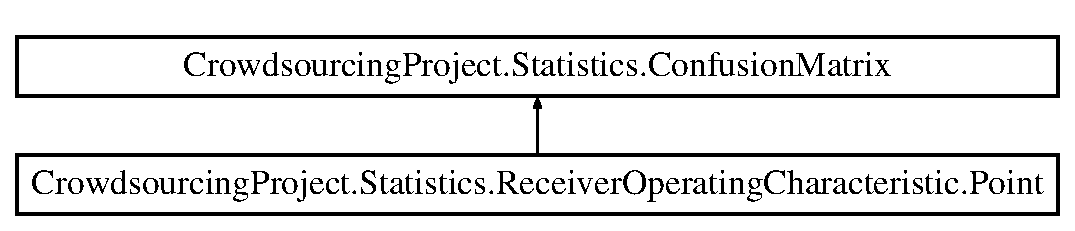
\includegraphics[height=2.000000cm]{class_crowdsourcing_project_1_1_statistics_1_1_receiver_operating_characteristic_1_1_point}
\end{center}
\end{figure}
\subsection*{Properties}
\begin{DoxyCompactItemize}
\item 
double \hyperlink{class_crowdsourcing_project_1_1_statistics_1_1_receiver_operating_characteristic_1_1_point_aba21bd4e1ac0f108580c8387eb8a933d}{Cutoff}\hspace{0.3cm}{\ttfamily  \mbox{[}get\mbox{]}}
\begin{DoxyCompactList}\small\item\em Gets the cutoff value (discrimination threshold) for this point. \end{DoxyCompactList}\end{DoxyCompactItemize}
\subsection*{Additional Inherited Members}


\subsection{Detailed Description}
Object to hold information about a Receiver Operating Characteristic Curve \hyperlink{class_crowdsourcing_project_1_1_statistics_1_1_receiver_operating_characteristic_1_1_point}{Point} 



\subsection{Property Documentation}
\hypertarget{class_crowdsourcing_project_1_1_statistics_1_1_receiver_operating_characteristic_1_1_point_aba21bd4e1ac0f108580c8387eb8a933d}{}\index{Crowdsourcing\+Project\+::\+Statistics\+::\+Receiver\+Operating\+Characteristic\+::\+Point@{Crowdsourcing\+Project\+::\+Statistics\+::\+Receiver\+Operating\+Characteristic\+::\+Point}!Cutoff@{Cutoff}}
\index{Cutoff@{Cutoff}!Crowdsourcing\+Project\+::\+Statistics\+::\+Receiver\+Operating\+Characteristic\+::\+Point@{Crowdsourcing\+Project\+::\+Statistics\+::\+Receiver\+Operating\+Characteristic\+::\+Point}}
\subsubsection[{Cutoff}]{\setlength{\rightskip}{0pt plus 5cm}double Crowdsourcing\+Project.\+Statistics.\+Receiver\+Operating\+Characteristic.\+Point.\+Cutoff\hspace{0.3cm}{\ttfamily [get]}}\label{class_crowdsourcing_project_1_1_statistics_1_1_receiver_operating_characteristic_1_1_point_aba21bd4e1ac0f108580c8387eb8a933d}


Gets the cutoff value (discrimination threshold) for this point. 



The documentation for this class was generated from the following file\+:\begin{DoxyCompactItemize}
\item 
C\+:/\+Users/\+Matteo/\+Source/\+Repos/active-\/crowd/\+Crowdsourcing\+Models/\+Statistics/Receiver\+Operating\+Characteristic.\+cs\end{DoxyCompactItemize}

\hypertarget{class_crowdsourcing_project_1_1_statistics_1_1_receiver_operating_characteristic_1_1_point_collection}{}\section{Crowdsourcing\+Project.\+Statistics.\+Receiver\+Operating\+Characteristic.\+Point\+Collection Class Reference}
\label{class_crowdsourcing_project_1_1_statistics_1_1_receiver_operating_characteristic_1_1_point_collection}\index{Crowdsourcing\+Project.\+Statistics.\+Receiver\+Operating\+Characteristic.\+Point\+Collection@{Crowdsourcing\+Project.\+Statistics.\+Receiver\+Operating\+Characteristic.\+Point\+Collection}}


Represents a Collection of Receiver Operating Characteristic (R\+O\+C) Curve points. This class cannot be instantiated.  


Inheritance diagram for Crowdsourcing\+Project.\+Statistics.\+Receiver\+Operating\+Characteristic.\+Point\+Collection\+:\begin{figure}[H]
\begin{center}
\leavevmode
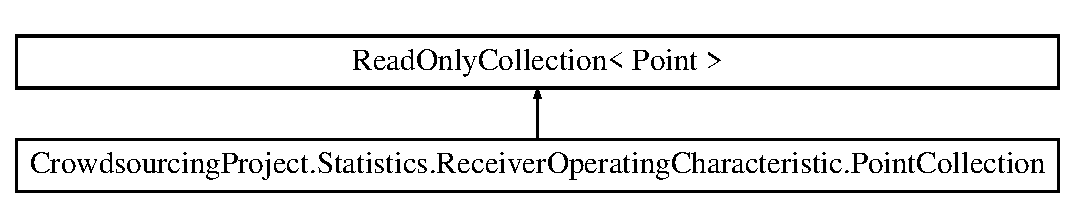
\includegraphics[height=2.000000cm]{class_crowdsourcing_project_1_1_statistics_1_1_receiver_operating_characteristic_1_1_point_collection}
\end{center}
\end{figure}


\subsection{Detailed Description}
Represents a Collection of Receiver Operating Characteristic (R\+O\+C) Curve points. This class cannot be instantiated. 



The documentation for this class was generated from the following file\+:\begin{DoxyCompactItemize}
\item 
C\+:/\+Users/\+Matteo/\+Source/\+Repos/active-\/crowd/\+Crowdsourcing\+Models/\+Statistics/Receiver\+Operating\+Characteristic.\+cs\end{DoxyCompactItemize}

\hypertarget{class_crowdsourcing_models_1_1_program}{}\section{Crowdsourcing\+Models.\+Program Class Reference}
\label{class_crowdsourcing_models_1_1_program}\index{Crowdsourcing\+Models.\+Program@{Crowdsourcing\+Models.\+Program}}


The class for the main program.  


\subsection*{Static Public Member Functions}
\begin{DoxyCompactItemize}
\item 
static \hyperlink{class_crowdsourcing_models_1_1_results}{Results} \hyperlink{class_crowdsourcing_models_1_1_program_a0c8aba76a474add91e7ae5a31afb3a14}{Run\+Gold} (string data\+Set, I\+List$<$ \hyperlink{class_crowdsourcing_models_1_1_datum}{Datum} $>$ data, \hyperlink{namespace_crowdsourcing_models_ae187d0e1d9fe64e7ebcb9d948d02d2d0}{Run\+Type} run\+Type, \hyperlink{class_crowdsourcing_models_1_1_b_c_c}{B\+C\+C} model, int num\+Communities=2)
\begin{DoxyCompactList}\small\item\em Runs a model with the full gold set. \end{DoxyCompactList}\item 
static string \hyperlink{class_crowdsourcing_models_1_1_program_a277c2d73fa1de5d400eb0ae1925c014f}{Get\+Model\+Name} (string dataset, \hyperlink{namespace_crowdsourcing_models_ae187d0e1d9fe64e7ebcb9d948d02d2d0}{Run\+Type} run\+Type, \hyperlink{namespace_crowdsourcing_models_a1bb21d66b6c86daa36af97d919528356}{Task\+Selection\+Method} task\+Selection\+Method, \hyperlink{namespace_crowdsourcing_models_a1f0e849dc0691caa8fda0ce7778756a6}{Worker\+Selection\+Method} worker\+Selection\+Method, int \hyperlink{class_crowdsourcing_models_1_1_program_aaf063cf9af3dc47e84aaab11562a5b12}{Num\+Communities})
\begin{DoxyCompactList}\small\item\em Returns the model name as a string. \end{DoxyCompactList}\item 
static string \hyperlink{class_crowdsourcing_models_1_1_program_a1c0be23ce716b7d30addb497a0185861}{Get\+Model\+Name} (string dataset, \hyperlink{namespace_crowdsourcing_models_ae187d0e1d9fe64e7ebcb9d948d02d2d0}{Run\+Type} run\+Type)
\begin{DoxyCompactList}\small\item\em Returns the model name as a string. \end{DoxyCompactList}\end{DoxyCompactItemize}
\subsection*{Static Public Attributes}
\begin{DoxyCompactItemize}
\item 
static string\mbox{[}$\,$\mbox{]} \hyperlink{class_crowdsourcing_models_1_1_program_a4055096a1a87c6ef001b0ebe0a1cc467}{Datasets} = new string\mbox{[}$\,$\mbox{]} \{ \char`\"{}C\+F\char`\"{}, \char`\"{}Zen\+Crowd\+\_\+us\char`\"{}, \char`\"{}Zen\+Crowd\+\_\+in\char`\"{} \}
\begin{DoxyCompactList}\small\item\em The datasets. \end{DoxyCompactList}\item 
\hypertarget{class_crowdsourcing_models_1_1_program_a47f427b18fe8fe4abf17cb01576b7b14}{}static bool {\bfseries Use\+Real\+Data}\label{class_crowdsourcing_models_1_1_program_a47f427b18fe8fe4abf17cb01576b7b14}

\item 
static int\mbox{[}$\,$\mbox{]} \hyperlink{class_crowdsourcing_models_1_1_program_aaf063cf9af3dc47e84aaab11562a5b12}{Num\+Communities} = new int\mbox{[}$\,$\mbox{]} \{ 4 \}
\begin{DoxyCompactList}\small\item\em The number of communities of \hyperlink{class_crowdsourcing_models_1_1_c_b_c_c}{C\+B\+C\+C}. \end{DoxyCompactList}\item 
static bool \hyperlink{class_crowdsourcing_models_1_1_program_a77ef65213ec54609ff34903232672a3d}{is\+Recorded\+To\+Txt\+File} = false
\begin{DoxyCompactList}\small\item\em Flag to redirect the console output to txt file \end{DoxyCompactList}\item 
\hypertarget{class_crowdsourcing_models_1_1_program_a94c9761dbe8926f9f0f7658a16291b6d}{}static int {\bfseries start\+Index} = 0\label{class_crowdsourcing_models_1_1_program_a94c9761dbe8926f9f0f7658a16291b6d}

\item 
\hypertarget{class_crowdsourcing_models_1_1_program_afd9a093c86071eaa4ba6f342c894a6af}{}static int {\bfseries end\+Index} = 0\label{class_crowdsourcing_models_1_1_program_afd9a093c86071eaa4ba6f342c894a6af}

\item 
\hypertarget{class_crowdsourcing_models_1_1_program_a07e68b7cfe03887103512b56e795b4da}{}static int {\bfseries which\+Model}\label{class_crowdsourcing_models_1_1_program_a07e68b7cfe03887103512b56e795b4da}

\item 
\hypertarget{class_crowdsourcing_models_1_1_program_a98ba4d910dfe8dfa76c981f7c0bc26f2}{}static int {\bfseries cluster\+Iter}\label{class_crowdsourcing_models_1_1_program_a98ba4d910dfe8dfa76c981f7c0bc26f2}

\end{DoxyCompactItemize}


\subsection{Detailed Description}
The class for the main program. 



\subsection{Member Function Documentation}
\hypertarget{class_crowdsourcing_models_1_1_program_a277c2d73fa1de5d400eb0ae1925c014f}{}\index{Crowdsourcing\+Models\+::\+Program@{Crowdsourcing\+Models\+::\+Program}!Get\+Model\+Name@{Get\+Model\+Name}}
\index{Get\+Model\+Name@{Get\+Model\+Name}!Crowdsourcing\+Models\+::\+Program@{Crowdsourcing\+Models\+::\+Program}}
\subsubsection[{Get\+Model\+Name(string dataset, Run\+Type run\+Type, Task\+Selection\+Method task\+Selection\+Method, Worker\+Selection\+Method worker\+Selection\+Method, int Num\+Communities)}]{\setlength{\rightskip}{0pt plus 5cm}static string Crowdsourcing\+Models.\+Program.\+Get\+Model\+Name (
\begin{DoxyParamCaption}
\item[{string}]{dataset, }
\item[{{\bf Run\+Type}}]{run\+Type, }
\item[{{\bf Task\+Selection\+Method}}]{task\+Selection\+Method, }
\item[{{\bf Worker\+Selection\+Method}}]{worker\+Selection\+Method, }
\item[{int}]{Num\+Communities}
\end{DoxyParamCaption}
)\hspace{0.3cm}{\ttfamily [inline]}, {\ttfamily [static]}}\label{class_crowdsourcing_models_1_1_program_a277c2d73fa1de5d400eb0ae1925c014f}


Returns the model name as a string. 


\begin{DoxyParams}{Parameters}
{\em dataset} & The name of the data set.\\
\hline
{\em run\+Type} & The model run type.\\
\hline
{\em task\+Selection\+Method} & The method for selecting tasks (Random / Entropy).\\
\hline
{\em worker\+Selection\+Method} & The method for selecting workers (only Random is implemented).\\
\hline
{\em num\+Communities} & The number of communities (only for \hyperlink{class_crowdsourcing_models_1_1_c_b_c_c}{C\+B\+C\+C}).\\
\hline
\end{DoxyParams}
\begin{DoxyReturn}{Returns}
The model name
\end{DoxyReturn}
\hypertarget{class_crowdsourcing_models_1_1_program_a1c0be23ce716b7d30addb497a0185861}{}\index{Crowdsourcing\+Models\+::\+Program@{Crowdsourcing\+Models\+::\+Program}!Get\+Model\+Name@{Get\+Model\+Name}}
\index{Get\+Model\+Name@{Get\+Model\+Name}!Crowdsourcing\+Models\+::\+Program@{Crowdsourcing\+Models\+::\+Program}}
\subsubsection[{Get\+Model\+Name(string dataset, Run\+Type run\+Type)}]{\setlength{\rightskip}{0pt plus 5cm}static string Crowdsourcing\+Models.\+Program.\+Get\+Model\+Name (
\begin{DoxyParamCaption}
\item[{string}]{dataset, }
\item[{{\bf Run\+Type}}]{run\+Type}
\end{DoxyParamCaption}
)\hspace{0.3cm}{\ttfamily [inline]}, {\ttfamily [static]}}\label{class_crowdsourcing_models_1_1_program_a1c0be23ce716b7d30addb497a0185861}


Returns the model name as a string. 


\begin{DoxyParams}{Parameters}
{\em dataset} & The name of the data set.\\
\hline
{\em run\+Type} & The model run type.\\
\hline
\end{DoxyParams}
\begin{DoxyReturn}{Returns}
The model name
\end{DoxyReturn}
\hypertarget{class_crowdsourcing_models_1_1_program_a0c8aba76a474add91e7ae5a31afb3a14}{}\index{Crowdsourcing\+Models\+::\+Program@{Crowdsourcing\+Models\+::\+Program}!Run\+Gold@{Run\+Gold}}
\index{Run\+Gold@{Run\+Gold}!Crowdsourcing\+Models\+::\+Program@{Crowdsourcing\+Models\+::\+Program}}
\subsubsection[{Run\+Gold(string data\+Set, I\+List$<$ Datum $>$ data, Run\+Type run\+Type, B\+C\+C model, int num\+Communities=2)}]{\setlength{\rightskip}{0pt plus 5cm}static {\bf Results} Crowdsourcing\+Models.\+Program.\+Run\+Gold (
\begin{DoxyParamCaption}
\item[{string}]{data\+Set, }
\item[{I\+List$<$ {\bf Datum} $>$}]{data, }
\item[{{\bf Run\+Type}}]{run\+Type, }
\item[{{\bf B\+C\+C}}]{model, }
\item[{int}]{num\+Communities = {\ttfamily 2}}
\end{DoxyParamCaption}
)\hspace{0.3cm}{\ttfamily [inline]}, {\ttfamily [static]}}\label{class_crowdsourcing_models_1_1_program_a0c8aba76a474add91e7ae5a31afb3a14}


Runs a model with the full gold set. 


\begin{DoxyParams}{Parameters}
{\em data\+Set} & The data.\\
\hline
{\em current\+Task\+Selection\+Method} & Current Task Selection Method\\
\hline
{\em run\+Type} & The model run type.\\
\hline
{\em model} & The model instance.\\
\hline
{\em num\+Communities} & The number of communities (only for \hyperlink{class_crowdsourcing_models_1_1_c_b_c_c}{C\+B\+C\+C}).\\
\hline
\end{DoxyParams}
\begin{DoxyReturn}{Returns}
The inference results
\end{DoxyReturn}


\subsection{Member Data Documentation}
\hypertarget{class_crowdsourcing_models_1_1_program_a4055096a1a87c6ef001b0ebe0a1cc467}{}\index{Crowdsourcing\+Models\+::\+Program@{Crowdsourcing\+Models\+::\+Program}!Datasets@{Datasets}}
\index{Datasets@{Datasets}!Crowdsourcing\+Models\+::\+Program@{Crowdsourcing\+Models\+::\+Program}}
\subsubsection[{Datasets}]{\setlength{\rightskip}{0pt plus 5cm}string \mbox{[}$\,$\mbox{]} Crowdsourcing\+Models.\+Program.\+Datasets = new string\mbox{[}$\,$\mbox{]} \{ \char`\"{}C\+F\char`\"{}, \char`\"{}Zen\+Crowd\+\_\+us\char`\"{}, \char`\"{}Zen\+Crowd\+\_\+in\char`\"{} \}\hspace{0.3cm}{\ttfamily [static]}}\label{class_crowdsourcing_models_1_1_program_a4055096a1a87c6ef001b0ebe0a1cc467}


The datasets. 

\hypertarget{class_crowdsourcing_models_1_1_program_a77ef65213ec54609ff34903232672a3d}{}\index{Crowdsourcing\+Models\+::\+Program@{Crowdsourcing\+Models\+::\+Program}!is\+Recorded\+To\+Txt\+File@{is\+Recorded\+To\+Txt\+File}}
\index{is\+Recorded\+To\+Txt\+File@{is\+Recorded\+To\+Txt\+File}!Crowdsourcing\+Models\+::\+Program@{Crowdsourcing\+Models\+::\+Program}}
\subsubsection[{is\+Recorded\+To\+Txt\+File}]{\setlength{\rightskip}{0pt plus 5cm}bool Crowdsourcing\+Models.\+Program.\+is\+Recorded\+To\+Txt\+File = false\hspace{0.3cm}{\ttfamily [static]}}\label{class_crowdsourcing_models_1_1_program_a77ef65213ec54609ff34903232672a3d}


Flag to redirect the console output to txt file 

\hypertarget{class_crowdsourcing_models_1_1_program_aaf063cf9af3dc47e84aaab11562a5b12}{}\index{Crowdsourcing\+Models\+::\+Program@{Crowdsourcing\+Models\+::\+Program}!Num\+Communities@{Num\+Communities}}
\index{Num\+Communities@{Num\+Communities}!Crowdsourcing\+Models\+::\+Program@{Crowdsourcing\+Models\+::\+Program}}
\subsubsection[{Num\+Communities}]{\setlength{\rightskip}{0pt plus 5cm}int \mbox{[}$\,$\mbox{]} Crowdsourcing\+Models.\+Program.\+Num\+Communities = new int\mbox{[}$\,$\mbox{]} \{ 4 \}\hspace{0.3cm}{\ttfamily [static]}}\label{class_crowdsourcing_models_1_1_program_aaf063cf9af3dc47e84aaab11562a5b12}


The number of communities of \hyperlink{class_crowdsourcing_models_1_1_c_b_c_c}{C\+B\+C\+C}. 



The documentation for this class was generated from the following file\+:\begin{DoxyCompactItemize}
\item 
C\+:/\+Users/\+Matteo/\+Source/\+Repos/active-\/crowd/\+Crowdsourcing\+Models/Program.\+cs\end{DoxyCompactItemize}

\hypertarget{class_crowdsourcing_project_1_1_statistics_1_1_receiver_operating_characteristic}{}\section{Crowdsourcing\+Project.\+Statistics.\+Receiver\+Operating\+Characteristic Class Reference}
\label{class_crowdsourcing_project_1_1_statistics_1_1_receiver_operating_characteristic}\index{Crowdsourcing\+Project.\+Statistics.\+Receiver\+Operating\+Characteristic@{Crowdsourcing\+Project.\+Statistics.\+Receiver\+Operating\+Characteristic}}


Receiver Operating Characteristic (R\+O\+C) Curve  


\subsection*{Classes}
\begin{DoxyCompactItemize}
\item 
class \hyperlink{class_crowdsourcing_project_1_1_statistics_1_1_receiver_operating_characteristic_1_1_point}{Point}
\begin{DoxyCompactList}\small\item\em Object to hold information about a Receiver Operating Characteristic Curve \hyperlink{class_crowdsourcing_project_1_1_statistics_1_1_receiver_operating_characteristic_1_1_point}{Point} \end{DoxyCompactList}\item 
class \hyperlink{class_crowdsourcing_project_1_1_statistics_1_1_receiver_operating_characteristic_1_1_point_collection}{Point\+Collection}
\begin{DoxyCompactList}\small\item\em Represents a Collection of Receiver Operating Characteristic (R\+O\+C) Curve points. This class cannot be instantiated. \end{DoxyCompactList}\end{DoxyCompactItemize}
\subsection*{Public Member Functions}
\begin{DoxyCompactItemize}
\item 
\hyperlink{class_crowdsourcing_project_1_1_statistics_1_1_receiver_operating_characteristic_a9a4c7b63ce6eee404b29ed49918f7f15}{Receiver\+Operating\+Characteristic} (double\mbox{[}$\,$\mbox{]} measurement, double\mbox{[}$\,$\mbox{]} prediction)
\begin{DoxyCompactList}\small\item\em Constructs a new Receiver Operating Characteristic model \end{DoxyCompactList}\item 
void \hyperlink{class_crowdsourcing_project_1_1_statistics_1_1_receiver_operating_characteristic_a6f85910fcec4797bcf43ffa280dfd539}{Compute} (int points)
\begin{DoxyCompactList}\small\item\em Computes a n-\/points R\+O\+C curve. \end{DoxyCompactList}\item 
void \hyperlink{class_crowdsourcing_project_1_1_statistics_1_1_receiver_operating_characteristic_a7fcfa4f4ede738aee8496d5b8ea5733f}{Compute} (double increment)
\begin{DoxyCompactList}\small\item\em Computes a R\+O\+C curve with 1/increment points \end{DoxyCompactList}\item 
double \hyperlink{class_crowdsourcing_project_1_1_statistics_1_1_receiver_operating_characteristic_a1f75eac7968344a9459f2903ded545cc}{Compare} (\hyperlink{class_crowdsourcing_project_1_1_statistics_1_1_receiver_operating_characteristic}{Receiver\+Operating\+Characteristic} curve, double r)
\begin{DoxyCompactList}\small\item\em Compares two R\+O\+C curves. \end{DoxyCompactList}\end{DoxyCompactItemize}
\subsection*{Public Attributes}
\begin{DoxyCompactItemize}
\item 
\hypertarget{class_crowdsourcing_project_1_1_statistics_1_1_receiver_operating_characteristic_a991d81f989e5822b615bc768f38143d8}{}\hyperlink{class_crowdsourcing_project_1_1_statistics_1_1_receiver_operating_characteristic_1_1_point_collection}{Point\+Collection} {\bfseries collection}\label{class_crowdsourcing_project_1_1_statistics_1_1_receiver_operating_characteristic_a991d81f989e5822b615bc768f38143d8}

\end{DoxyCompactItemize}
\subsection*{Properties}
\begin{DoxyCompactItemize}
\item 
\hyperlink{class_crowdsourcing_project_1_1_statistics_1_1_receiver_operating_characteristic_1_1_point_collection}{Point\+Collection} \hyperlink{class_crowdsourcing_project_1_1_statistics_1_1_receiver_operating_characteristic_a0684231949d27fe15a40af511cedfa1e}{Points}\hspace{0.3cm}{\ttfamily  \mbox{[}get\mbox{]}}
\begin{DoxyCompactList}\small\item\em Gets the points of the curve. \end{DoxyCompactList}\item 
double \hyperlink{class_crowdsourcing_project_1_1_statistics_1_1_receiver_operating_characteristic_ac7cd3193e58dddd982b54b39a3284e1f}{Area}\hspace{0.3cm}{\ttfamily  \mbox{[}get\mbox{]}}
\begin{DoxyCompactList}\small\item\em The area under the R\+O\+C curve. Also known as A\+U\+C-\/\+R\+O\+C. \end{DoxyCompactList}\item 
double \hyperlink{class_crowdsourcing_project_1_1_statistics_1_1_receiver_operating_characteristic_a122e8eb0e99a3b298f7370736114511a}{Error}\hspace{0.3cm}{\ttfamily  \mbox{[}get\mbox{]}}
\begin{DoxyCompactList}\small\item\em Calculates the Standard Error associated with this R\+O\+C curve. \end{DoxyCompactList}\end{DoxyCompactItemize}


\subsection{Detailed Description}
Receiver Operating Characteristic (R\+O\+C) Curve 

In signal detection theory, a receiver operating characteristic (R\+O\+C), or simply R\+O\+C curve, is a graphical plot of the sensitivity vs. (1 − specificity) for a binary classifier system as its discrimination threshold is varied.

References\+: \href{http://en.wikipedia.org/wiki/Receiver_operating_characteristic}{\tt http\+://en.\+wikipedia.\+org/wiki/\+Receiver\+\_\+operating\+\_\+characteristic} \href{http://www.anaesthetist.com/mnm/stats/roc/Findex.htm}{\tt http\+://www.\+anaesthetist.\+com/mnm/stats/roc/\+Findex.\+htm} \href{http://radiology.rsna.org/content/148/3/839.full.pdf}{\tt http\+://radiology.\+rsna.\+org/content/148/3/839.\+full.\+pdf} 

\subsection{Constructor \& Destructor Documentation}
\hypertarget{class_crowdsourcing_project_1_1_statistics_1_1_receiver_operating_characteristic_a9a4c7b63ce6eee404b29ed49918f7f15}{}\index{Crowdsourcing\+Project\+::\+Statistics\+::\+Receiver\+Operating\+Characteristic@{Crowdsourcing\+Project\+::\+Statistics\+::\+Receiver\+Operating\+Characteristic}!Receiver\+Operating\+Characteristic@{Receiver\+Operating\+Characteristic}}
\index{Receiver\+Operating\+Characteristic@{Receiver\+Operating\+Characteristic}!Crowdsourcing\+Project\+::\+Statistics\+::\+Receiver\+Operating\+Characteristic@{Crowdsourcing\+Project\+::\+Statistics\+::\+Receiver\+Operating\+Characteristic}}
\subsubsection[{Receiver\+Operating\+Characteristic(double[] measurement, double[] prediction)}]{\setlength{\rightskip}{0pt plus 5cm}Crowdsourcing\+Project.\+Statistics.\+Receiver\+Operating\+Characteristic.\+Receiver\+Operating\+Characteristic (
\begin{DoxyParamCaption}
\item[{double\mbox{[}$\,$\mbox{]}}]{measurement, }
\item[{double\mbox{[}$\,$\mbox{]}}]{prediction}
\end{DoxyParamCaption}
)\hspace{0.3cm}{\ttfamily [inline]}}\label{class_crowdsourcing_project_1_1_statistics_1_1_receiver_operating_characteristic_a9a4c7b63ce6eee404b29ed49918f7f15}


Constructs a new Receiver Operating Characteristic model 


\begin{DoxyParams}{Parameters}
{\em output} & An array of binary values. Tipically 0 and 1, or -\/1 and 1, indicating negative and positive cases, respectively.\\
\hline
{\em predicted\+Output} & An array of continuous values trying to approximate the measurement array.\\
\hline
\end{DoxyParams}


\subsection{Member Function Documentation}
\hypertarget{class_crowdsourcing_project_1_1_statistics_1_1_receiver_operating_characteristic_a1f75eac7968344a9459f2903ded545cc}{}\index{Crowdsourcing\+Project\+::\+Statistics\+::\+Receiver\+Operating\+Characteristic@{Crowdsourcing\+Project\+::\+Statistics\+::\+Receiver\+Operating\+Characteristic}!Compare@{Compare}}
\index{Compare@{Compare}!Crowdsourcing\+Project\+::\+Statistics\+::\+Receiver\+Operating\+Characteristic@{Crowdsourcing\+Project\+::\+Statistics\+::\+Receiver\+Operating\+Characteristic}}
\subsubsection[{Compare(\+Receiver\+Operating\+Characteristic curve, double r)}]{\setlength{\rightskip}{0pt plus 5cm}double Crowdsourcing\+Project.\+Statistics.\+Receiver\+Operating\+Characteristic.\+Compare (
\begin{DoxyParamCaption}
\item[{{\bf Receiver\+Operating\+Characteristic}}]{curve, }
\item[{double}]{r}
\end{DoxyParamCaption}
)\hspace{0.3cm}{\ttfamily [inline]}}\label{class_crowdsourcing_project_1_1_statistics_1_1_receiver_operating_characteristic_a1f75eac7968344a9459f2903ded545cc}


Compares two R\+O\+C curves. 


\begin{DoxyParams}{Parameters}
{\em r} & The amount of correlation between the two curves\\
\hline
\end{DoxyParams}
\begin{DoxyReturn}{Returns}

\end{DoxyReturn}
\hypertarget{class_crowdsourcing_project_1_1_statistics_1_1_receiver_operating_characteristic_a6f85910fcec4797bcf43ffa280dfd539}{}\index{Crowdsourcing\+Project\+::\+Statistics\+::\+Receiver\+Operating\+Characteristic@{Crowdsourcing\+Project\+::\+Statistics\+::\+Receiver\+Operating\+Characteristic}!Compute@{Compute}}
\index{Compute@{Compute}!Crowdsourcing\+Project\+::\+Statistics\+::\+Receiver\+Operating\+Characteristic@{Crowdsourcing\+Project\+::\+Statistics\+::\+Receiver\+Operating\+Characteristic}}
\subsubsection[{Compute(int points)}]{\setlength{\rightskip}{0pt plus 5cm}void Crowdsourcing\+Project.\+Statistics.\+Receiver\+Operating\+Characteristic.\+Compute (
\begin{DoxyParamCaption}
\item[{int}]{points}
\end{DoxyParamCaption}
)\hspace{0.3cm}{\ttfamily [inline]}}\label{class_crowdsourcing_project_1_1_statistics_1_1_receiver_operating_characteristic_a6f85910fcec4797bcf43ffa280dfd539}


Computes a n-\/points R\+O\+C curve. 

Each point in the R\+O\+C curve will have a threshold increase of 1/npoints over the previous point, starting at zero. 


\begin{DoxyParams}{Parameters}
{\em points} & The number of points for the curve.\\
\hline
\end{DoxyParams}
\hypertarget{class_crowdsourcing_project_1_1_statistics_1_1_receiver_operating_characteristic_a7fcfa4f4ede738aee8496d5b8ea5733f}{}\index{Crowdsourcing\+Project\+::\+Statistics\+::\+Receiver\+Operating\+Characteristic@{Crowdsourcing\+Project\+::\+Statistics\+::\+Receiver\+Operating\+Characteristic}!Compute@{Compute}}
\index{Compute@{Compute}!Crowdsourcing\+Project\+::\+Statistics\+::\+Receiver\+Operating\+Characteristic@{Crowdsourcing\+Project\+::\+Statistics\+::\+Receiver\+Operating\+Characteristic}}
\subsubsection[{Compute(double increment)}]{\setlength{\rightskip}{0pt plus 5cm}void Crowdsourcing\+Project.\+Statistics.\+Receiver\+Operating\+Characteristic.\+Compute (
\begin{DoxyParamCaption}
\item[{double}]{increment}
\end{DoxyParamCaption}
)\hspace{0.3cm}{\ttfamily [inline]}}\label{class_crowdsourcing_project_1_1_statistics_1_1_receiver_operating_characteristic_a7fcfa4f4ede738aee8496d5b8ea5733f}


Computes a R\+O\+C curve with 1/increment points 


\begin{DoxyParams}{Parameters}
{\em increment} & The increment over the previous point for each point in the curve.\\
\hline
\end{DoxyParams}


\subsection{Property Documentation}
\hypertarget{class_crowdsourcing_project_1_1_statistics_1_1_receiver_operating_characteristic_ac7cd3193e58dddd982b54b39a3284e1f}{}\index{Crowdsourcing\+Project\+::\+Statistics\+::\+Receiver\+Operating\+Characteristic@{Crowdsourcing\+Project\+::\+Statistics\+::\+Receiver\+Operating\+Characteristic}!Area@{Area}}
\index{Area@{Area}!Crowdsourcing\+Project\+::\+Statistics\+::\+Receiver\+Operating\+Characteristic@{Crowdsourcing\+Project\+::\+Statistics\+::\+Receiver\+Operating\+Characteristic}}
\subsubsection[{Area}]{\setlength{\rightskip}{0pt plus 5cm}double Crowdsourcing\+Project.\+Statistics.\+Receiver\+Operating\+Characteristic.\+Area\hspace{0.3cm}{\ttfamily [get]}}\label{class_crowdsourcing_project_1_1_statistics_1_1_receiver_operating_characteristic_ac7cd3193e58dddd982b54b39a3284e1f}


The area under the R\+O\+C curve. Also known as A\+U\+C-\/\+R\+O\+C. 

\hypertarget{class_crowdsourcing_project_1_1_statistics_1_1_receiver_operating_characteristic_a122e8eb0e99a3b298f7370736114511a}{}\index{Crowdsourcing\+Project\+::\+Statistics\+::\+Receiver\+Operating\+Characteristic@{Crowdsourcing\+Project\+::\+Statistics\+::\+Receiver\+Operating\+Characteristic}!Error@{Error}}
\index{Error@{Error}!Crowdsourcing\+Project\+::\+Statistics\+::\+Receiver\+Operating\+Characteristic@{Crowdsourcing\+Project\+::\+Statistics\+::\+Receiver\+Operating\+Characteristic}}
\subsubsection[{Error}]{\setlength{\rightskip}{0pt plus 5cm}double Crowdsourcing\+Project.\+Statistics.\+Receiver\+Operating\+Characteristic.\+Error\hspace{0.3cm}{\ttfamily [get]}}\label{class_crowdsourcing_project_1_1_statistics_1_1_receiver_operating_characteristic_a122e8eb0e99a3b298f7370736114511a}


Calculates the Standard Error associated with this R\+O\+C curve. 

\hypertarget{class_crowdsourcing_project_1_1_statistics_1_1_receiver_operating_characteristic_a0684231949d27fe15a40af511cedfa1e}{}\index{Crowdsourcing\+Project\+::\+Statistics\+::\+Receiver\+Operating\+Characteristic@{Crowdsourcing\+Project\+::\+Statistics\+::\+Receiver\+Operating\+Characteristic}!Points@{Points}}
\index{Points@{Points}!Crowdsourcing\+Project\+::\+Statistics\+::\+Receiver\+Operating\+Characteristic@{Crowdsourcing\+Project\+::\+Statistics\+::\+Receiver\+Operating\+Characteristic}}
\subsubsection[{Points}]{\setlength{\rightskip}{0pt plus 5cm}{\bf Point\+Collection} Crowdsourcing\+Project.\+Statistics.\+Receiver\+Operating\+Characteristic.\+Points\hspace{0.3cm}{\ttfamily [get]}}\label{class_crowdsourcing_project_1_1_statistics_1_1_receiver_operating_characteristic_a0684231949d27fe15a40af511cedfa1e}


Gets the points of the curve. 



The documentation for this class was generated from the following file\+:\begin{DoxyCompactItemize}
\item 
C\+:/\+Users/\+Matteo/\+Source/\+Repos/active-\/crowd/\+Crowdsourcing\+Models/\+Statistics/Receiver\+Operating\+Characteristic.\+cs\end{DoxyCompactItemize}

\hypertarget{class_crowdsourcing_models_1_1_results}{}\section{Crowdsourcing\+Models.\+Results Class Reference}
\label{class_crowdsourcing_models_1_1_results}\index{Crowdsourcing\+Models.\+Results@{Crowdsourcing\+Models.\+Results}}
\subsection*{Classes}
\begin{DoxyCompactItemize}
\item 
struct \hyperlink{struct_crowdsourcing_models_1_1_results_1_1_non_task_worker_parameters}{Non\+Task\+Worker\+Parameters}
\end{DoxyCompactItemize}
\subsection*{Public Member Functions}
\begin{DoxyCompactItemize}
\item 
\hyperlink{class_crowdsourcing_models_1_1_results}{Results} \hyperlink{class_crowdsourcing_models_1_1_results_a9675f99c4cd7bfbe2229bc779fd1fab3}{Run\+Majority\+Vote} (I\+List$<$ \hyperlink{class_crowdsourcing_models_1_1_datum}{Datum} $>$ data, I\+List$<$ \hyperlink{class_crowdsourcing_models_1_1_datum}{Datum} $>$ full\+Data, bool calculate\+Accuracy, bool use\+Vote\+Distribution)
\begin{DoxyCompactList}\small\item\em Runs the majority vote method on the data. \end{DoxyCompactList}\item 
\hyperlink{class_crowdsourcing_models_1_1_results}{Results} \hyperlink{class_crowdsourcing_models_1_1_results_a1b0640e55fe37434f6afb2baad374519}{Run\+Dawid\+Skene} (I\+List$<$ \hyperlink{class_crowdsourcing_models_1_1_datum}{Datum} $>$ data, I\+List$<$ \hyperlink{class_crowdsourcing_models_1_1_datum}{Datum} $>$ full\+Data, bool calculate\+Accuracy)
\begin{DoxyCompactList}\small\item\em Run Dawid-\/\+Skene on the data. \end{DoxyCompactList}\item 
\hypertarget{class_crowdsourcing_models_1_1_results_a9604afa801fe1c5d55429f67043dd135}{}void {\bfseries Run\+B\+C\+C} (string model\+Name, I\+List$<$ \hyperlink{class_crowdsourcing_models_1_1_datum}{Datum} $>$ data, I\+List$<$ \hyperlink{class_crowdsourcing_models_1_1_datum}{Datum} $>$ full\+Data, \hyperlink{class_crowdsourcing_models_1_1_b_c_c}{B\+C\+C} model, \hyperlink{namespace_crowdsourcing_models_ac2299b85781ea82aa2c8850723c8a063}{Run\+Mode} mode, bool calculate\+Accuracy, int num\+Communities=-\/1, bool serialize=false, bool serialize\+Community\+Posteriors=false)\label{class_crowdsourcing_models_1_1_results_a9604afa801fe1c5d55429f67043dd135}

\item 
\hypertarget{class_crowdsourcing_models_1_1_results_a0741d9be4c6af7f634d7f88df02ac2c0}{}void {\bfseries Write\+Basic\+Statistics} (Stream\+Writer writer)\label{class_crowdsourcing_models_1_1_results_a0741d9be4c6af7f634d7f88df02ac2c0}

\item 
\hypertarget{class_crowdsourcing_models_1_1_results_a4aacf633a2db5d0bf1df5d2d5e9b62e2}{}virtual void {\bfseries Write\+Results} (Stream\+Writer writer, bool write\+Community\+Parameters, bool write\+Worker\+Parameters, bool write\+Worker\+Communities)\label{class_crowdsourcing_models_1_1_results_a4aacf633a2db5d0bf1df5d2d5e9b62e2}

\item 
\hypertarget{class_crowdsourcing_models_1_1_results_a5671a2613a1ac145ea46714be55fe6f9}{}virtual void {\bfseries Write\+Accuracy} (Stream\+Writer writer)\label{class_crowdsourcing_models_1_1_results_a5671a2613a1ac145ea46714be55fe6f9}

\item 
double\mbox{[},\mbox{]} \hyperlink{class_crowdsourcing_models_1_1_results_addf80aff1622db41d84d077d9aaddfbb}{Get\+Confusion\+Matrices} (string worker\+Id=\char`\"{}\char`\"{}, int community\+Index=-\/1)
\item 
Discrete \hyperlink{class_crowdsourcing_models_1_1_results_aa9600574fa6802c4a2703ecc1e27d73a}{get\+Task\+True\+Label} (string task\+Id)
\begin{DoxyCompactList}\small\item\em Get True Label values of the given task\+Id \end{DoxyCompactList}\end{DoxyCompactItemize}
\subsection*{Static Public Member Functions}
\begin{DoxyCompactItemize}
\item 
\hypertarget{class_crowdsourcing_models_1_1_results_ad84f5e51fdbb8934e2028965743f36b8}{}static double\mbox{[}$\,$\mbox{]} {\bfseries Get\+Confusion\+Matrix\+Diagonal} (Vector\mbox{[}$\,$\mbox{]} confusion\+Matrix\+Mean)\label{class_crowdsourcing_models_1_1_results_ad84f5e51fdbb8934e2028965743f36b8}

\item 
\hypertarget{class_crowdsourcing_models_1_1_results_ac5ec09f57d9177d414c2ae6e9155f631}{}static void {\bfseries Write\+Confusion\+Matrix} (Stream\+Writer writer, string worker, Dirichlet\mbox{[}$\,$\mbox{]} confusion\+Matrix)\label{class_crowdsourcing_models_1_1_results_ac5ec09f57d9177d414c2ae6e9155f631}

\item 
\hypertarget{class_crowdsourcing_models_1_1_results_ae5556eb0e898f4f991c51668350efa08}{}static void {\bfseries Write\+Worker\+Confusion\+Matrix} (Stream\+Writer writer, string worker, double\mbox{[},\mbox{]} confusion\+Matrix)\label{class_crowdsourcing_models_1_1_results_ae5556eb0e898f4f991c51668350efa08}

\item 
\hypertarget{class_crowdsourcing_models_1_1_results_ae5f852bf1ad4581c667c7aa5b0235320}{}static void {\bfseries Write\+Worker\+Confusion\+Matrix} (Stream\+Writer writer, string worker, Vector\mbox{[}$\,$\mbox{]} confusion\+Matrix)\label{class_crowdsourcing_models_1_1_results_ae5f852bf1ad4581c667c7aa5b0235320}

\item 
\hypertarget{class_crowdsourcing_models_1_1_results_a53a1a91b8f91b8c206acf44b01a29cab}{}static string {\bfseries Get\+Model\+Name} (string dataset, \hyperlink{namespace_crowdsourcing_models_ae187d0e1d9fe64e7ebcb9d948d02d2d0}{Run\+Type} run\+Type, \hyperlink{namespace_crowdsourcing_models_a1bb21d66b6c86daa36af97d919528356}{Task\+Selection\+Method} task\+Selection\+Metric, \hyperlink{namespace_crowdsourcing_models_a1f0e849dc0691caa8fda0ce7778756a6}{Worker\+Selection\+Method} worker\+Selection\+Metric, bool online, int task\+Samples=-\/1, int worker\+Samples=-\/1, int num\+Communities=-\/1)\label{class_crowdsourcing_models_1_1_results_a53a1a91b8f91b8c206acf44b01a29cab}

\end{DoxyCompactItemize}
\subsection*{Protected Member Functions}
\begin{DoxyCompactItemize}
\item 
\hypertarget{class_crowdsourcing_models_1_1_results_a2571bb4f6789430a83286b96e0d8059d}{}virtual void {\bfseries Clear\+Results} ()\label{class_crowdsourcing_models_1_1_results_a2571bb4f6789430a83286b96e0d8059d}

\item 
\hypertarget{class_crowdsourcing_models_1_1_results_a34576e53d2a70c54862fa350f0cb87d7}{}virtual void {\bfseries Update\+Results} (\hyperlink{class_crowdsourcing_models_1_1_b_c_c_posteriors}{B\+C\+C\+Posteriors} posteriors, \hyperlink{namespace_crowdsourcing_models_ac2299b85781ea82aa2c8850723c8a063}{Run\+Mode} mode)\label{class_crowdsourcing_models_1_1_results_a34576e53d2a70c54862fa350f0cb87d7}

\item 
virtual void \hyperlink{class_crowdsourcing_models_1_1_results_aabeef9fdac232ed2f8a904f3c15d2e0e}{Update\+Accuracy} ()
\begin{DoxyCompactList}\small\item\em Updates the accuracy using the current results. \end{DoxyCompactList}\end{DoxyCompactItemize}
\subsection*{Properties}
\begin{DoxyCompactItemize}
\item 
Dictionary$<$ string, Discrete $>$ \hyperlink{class_crowdsourcing_models_1_1_results_a140d71795dcea434130891de21d6747b}{True\+Label}\hspace{0.3cm}{\ttfamily  \mbox{[}get, protected set\mbox{]}}
\begin{DoxyCompactList}\small\item\em The posterior of the true label for each task. \end{DoxyCompactList}\item 
Dictionary$<$ string, Discrete $>$ \hyperlink{class_crowdsourcing_models_1_1_results_afc8f124040ec1cb49c569bae611aaa93}{Look\+Ahead\+True\+Label}\hspace{0.3cm}{\ttfamily  \mbox{[}get, protected set\mbox{]}}
\begin{DoxyCompactList}\small\item\em The predicted label for each task when doing simulations from the current model state. It avoids overwriting the true label posterior. \end{DoxyCompactList}\item 
Dictionary$<$ string, Discrete $>$ \hyperlink{class_crowdsourcing_models_1_1_results_a63c41834f4a0f9ecf4403594ae2f2cdc}{True\+Label\+Constraint}\hspace{0.3cm}{\ttfamily  \mbox{[}get, protected set\mbox{]}}
\begin{DoxyCompactList}\small\item\em The posterior for the constraint that allows online learning for the true label variable. \end{DoxyCompactList}\item 
Dictionary$<$ string, int?$>$ \hyperlink{class_crowdsourcing_models_1_1_results_ae5a5447d6999e2afe99d68dfa839daa5}{Predicted\+Label}\hspace{0.3cm}{\ttfamily  \mbox{[}get, protected set\mbox{]}}
\begin{DoxyCompactList}\small\item\em The predicted label for each task \end{DoxyCompactList}\item 
Dirichlet \hyperlink{class_crowdsourcing_models_1_1_results_ae14a29a61a13b39d0de986a4c7045df4}{Background\+Label\+Prob}\hspace{0.3cm}{\ttfamily  \mbox{[}get, protected set\mbox{]}}
\begin{DoxyCompactList}\small\item\em The probabilities that generate the true label of all the tasks. \end{DoxyCompactList}\item 
Dictionary$<$ string, Dirichlet\mbox{[}$\,$\mbox{]}$>$ \hyperlink{class_crowdsourcing_models_1_1_results_aeacd6050969e57759ccefe7760abfdff}{Worker\+Confusion\+Matrix}\hspace{0.3cm}{\ttfamily  \mbox{[}get, protected set\mbox{]}}
\begin{DoxyCompactList}\small\item\em The posterior of the confusion matrix of each worker. \end{DoxyCompactList}\item 
Dictionary$<$ string, Vector\mbox{[}$\,$\mbox{]}$>$ \hyperlink{class_crowdsourcing_models_1_1_results_a3f83c2aa1c8067278b72de879e2683df}{Worker\+Confusion\+Matrix\+Mean}\hspace{0.3cm}{\ttfamily  \mbox{[}get, protected set\mbox{]}}
\begin{DoxyCompactList}\small\item\em The mean of the posterior of the confusion matrix of each worker. \end{DoxyCompactList}\item 
Dictionary$<$ string, Dirichlet\mbox{[}$\,$\mbox{]}$>$ \hyperlink{class_crowdsourcing_models_1_1_results_a8c9bb0c3660f32404b453c169bb4e2e3}{Look\+Ahead\+Worker\+Confusion\+Matrix}\hspace{0.3cm}{\ttfamily  \mbox{[}get, protected set\mbox{]}}
\begin{DoxyCompactList}\small\item\em The look-\/ahead posterior of the confusion matrix of each worker obtained after simulating a new label in look-\/ahead run mode. \end{DoxyCompactList}\item 
Dictionary$<$ string, Dictionary$<$ string, Discrete $>$ $>$ \hyperlink{class_crowdsourcing_models_1_1_results_ade5b969fe6b048391a8da32cc1f9a113}{Worker\+Prediction}\hspace{0.3cm}{\ttfamily  \mbox{[}get, protected set\mbox{]}}
\begin{DoxyCompactList}\small\item\em The predictive probabilities of the labels produced by each worker. \end{DoxyCompactList}\item 
Dictionary$<$ string, Discrete $>$ \hyperlink{class_crowdsourcing_models_1_1_results_a898393862d585cafb14aa6a2d617641e}{Worker\+Community}\hspace{0.3cm}{\ttfamily  \mbox{[}get, protected set\mbox{]}}
\begin{DoxyCompactList}\small\item\em The community membership probabilities of each worker. \end{DoxyCompactList}\item 
Dirichlet\mbox{[}$\,$\mbox{]}\mbox{[}$\,$\mbox{]} \hyperlink{class_crowdsourcing_models_1_1_results_ad0d0152603265575be53ab612f892b6e}{Community\+Confusion\+Matrix}\hspace{0.3cm}{\ttfamily  \mbox{[}get, protected set\mbox{]}}
\begin{DoxyCompactList}\small\item\em The confusion matrix of each community. \end{DoxyCompactList}\item 
Vector\+Gaussian\mbox{[}$\,$\mbox{]}\mbox{[}$\,$\mbox{]} \hyperlink{class_crowdsourcing_models_1_1_results_ac7537fa71a408a747852b7970805dc91}{Community\+Score\+Matrix}\hspace{0.3cm}{\ttfamily  \mbox{[}get, protected set\mbox{]}}
\begin{DoxyCompactList}\small\item\em The score matrix of each community. \end{DoxyCompactList}\item 
Dictionary$<$ string, Vector\+Gaussian\mbox{[}$\,$\mbox{]}$>$ \hyperlink{class_crowdsourcing_models_1_1_results_acf297b7ce2319208a4875c77ca6aa535}{Worker\+Score\+Matrix\+Constraint}\hspace{0.3cm}{\ttfamily  \mbox{[}get, protected set\mbox{]}}
\begin{DoxyCompactList}\small\item\em The posterior for the constraint that allows online learning for worker confusion matrices int the community model. \end{DoxyCompactList}\item 
Dirichlet \hyperlink{class_crowdsourcing_models_1_1_results_af44b21781d8413575f1196752ec04851}{Community\+Prob}\hspace{0.3cm}{\ttfamily  \mbox{[}get, protected set\mbox{]}}
\begin{DoxyCompactList}\small\item\em The probabilities that generate the community memberships of all the workers. \end{DoxyCompactList}\item 
Dictionary$<$ string, Discrete $>$ \hyperlink{class_crowdsourcing_models_1_1_results_a71e11daa6e177bb987bb488c576e5ac5}{Community\+Constraint}\hspace{0.3cm}{\ttfamily  \mbox{[}get, protected set\mbox{]}}
\begin{DoxyCompactList}\small\item\em The posterior for the constraint that allows online learning for community membership. int the community model. \end{DoxyCompactList}\item 
Bernoulli \hyperlink{class_crowdsourcing_models_1_1_results_ad7d3df074d2f06c1d4c979a03b371e98}{Model\+Evidence}\hspace{0.3cm}{\ttfamily  \mbox{[}get, protected set\mbox{]}}
\begin{DoxyCompactList}\small\item\em Model evidence. \end{DoxyCompactList}\item 
\hyperlink{class_crowdsourcing_models_1_1_data_mapping}{Data\+Mapping} \hyperlink{class_crowdsourcing_models_1_1_results_ad5b164d844e8bace19604f8cf056e4fe}{Mapping}\hspace{0.3cm}{\ttfamily  \mbox{[}get, set\mbox{]}}
\begin{DoxyCompactList}\small\item\em The data mapping. \end{DoxyCompactList}\item 
\hyperlink{class_crowdsourcing_models_1_1_data_mapping}{Data\+Mapping} \hyperlink{class_crowdsourcing_models_1_1_results_a8ec786eadd78965d983b08cc44a650dc}{Full\+Mapping}\hspace{0.3cm}{\ttfamily  \mbox{[}get, set\mbox{]}}
\begin{DoxyCompactList}\small\item\em The full data mapping. \end{DoxyCompactList}\item 
Dictionary$<$ string, int?$>$ \hyperlink{class_crowdsourcing_models_1_1_results_a25fe8942765452821d24ed2b7fe9a472}{Gold\+Labels}\hspace{0.3cm}{\ttfamily  \mbox{[}get, protected set\mbox{]}}
\begin{DoxyCompactList}\small\item\em The gold labels of each task. The gold label type is nullable to support the (usual) situation where the is no labels. \end{DoxyCompactList}\item 
double \hyperlink{class_crowdsourcing_models_1_1_results_a0ae7118c643ec96ed7cf4f05db48c562}{Accuracy}\hspace{0.3cm}{\ttfamily  \mbox{[}get\mbox{]}}
\begin{DoxyCompactList}\small\item\em The accuracy of the current true label predictions. \end{DoxyCompactList}\item 
double \hyperlink{class_crowdsourcing_models_1_1_results_aab75338f84a6d1110365817b68691d4f}{Worker\+Label\+Accuracy}\hspace{0.3cm}{\ttfamily  \mbox{[}get, protected set\mbox{]}}
\begin{DoxyCompactList}\small\item\em The accuracy of the worker labels. \end{DoxyCompactList}\item 
double \hyperlink{class_crowdsourcing_models_1_1_results_a61808b2f35c5c4f739ed37eef609bfef}{Negative\+Log\+Prob}\hspace{0.3cm}{\ttfamily  \mbox{[}get\mbox{]}}
\begin{DoxyCompactList}\small\item\em The negative log probability density (N\+L\+P\+D) scores of the current true label predictions. \end{DoxyCompactList}\item 
double \hyperlink{class_crowdsourcing_models_1_1_results_a578be0205d443ac94124b8f7b89caa74}{Avg\+Recall}\hspace{0.3cm}{\ttfamily  \mbox{[}get\mbox{]}}
\begin{DoxyCompactList}\small\item\em The average recall of the current true label predictions. \end{DoxyCompactList}\item 
double\mbox{[},\mbox{]} \hyperlink{class_crowdsourcing_models_1_1_results_a3743219650ac6c051e146aa6c628da13}{Model\+Confusion\+Matrix}\hspace{0.3cm}{\ttfamily  \mbox{[}get\mbox{]}}
\begin{DoxyCompactList}\small\item\em The confusion matrix of the predicted true labels against the gold labels The rows are the gold labels and the columns are the predicted labels. \end{DoxyCompactList}\item 
bool \hyperlink{class_crowdsourcing_models_1_1_results_a87952670327f4e18a4183dab7238c3d4}{Is\+Community\+Model}\hspace{0.3cm}{\ttfamily  \mbox{[}get\mbox{]}}
\begin{DoxyCompactList}\small\item\em Flags whether the model instance is \hyperlink{class_crowdsourcing_models_1_1_c_b_c_c}{C\+B\+C\+C} (true) or \hyperlink{class_crowdsourcing_models_1_1_b_c_c}{B\+C\+C} (false). \end{DoxyCompactList}\item 
bool \hyperlink{class_crowdsourcing_models_1_1_results_a9b530081d9a4d406f071c7a3e8e3fb71}{Is\+Time\+Model}\hspace{0.3cm}{\ttfamily  \mbox{[}get\mbox{]}}
\begin{DoxyCompactList}\small\item\em Flags whether the model instance is a \hyperlink{class_crowdsourcing_models_1_1_b_c_c}{B\+C\+C} time model (true) or not (false). \end{DoxyCompactList}\item 
bool \hyperlink{class_crowdsourcing_models_1_1_results_a0ddff489da9fc4daab54d8fcc7163acb}{Is\+Time\+Multimode\+Model}\hspace{0.3cm}{\ttfamily  \mbox{[}get\mbox{]}}
\begin{DoxyCompactList}\small\item\em Flags whether the model instance is a \hyperlink{class_crowdsourcing_models_1_1_b_c_c}{B\+C\+C} time model (true) or not (false). \end{DoxyCompactList}\item 
\hypertarget{class_crowdsourcing_models_1_1_results_a73c4db10877ad67456a71f60dc687188}{}bool {\bfseries Is\+Time\+Task\+Propensity\+Model}\hspace{0.3cm}{\ttfamily  \mbox{[}get\mbox{]}}\label{class_crowdsourcing_models_1_1_results_a73c4db10877ad67456a71f60dc687188}

\item 
int \hyperlink{class_crowdsourcing_models_1_1_results_a90fd0653bd49b69cc9f12ad7cfb3fa9c}{Community\+Count}\hspace{0.3cm}{\ttfamily  \mbox{[}get\mbox{]}}
\begin{DoxyCompactList}\small\item\em The number of communities. \end{DoxyCompactList}\item 
\hypertarget{class_crowdsourcing_models_1_1_results_ab48ec731c1dcda12ec18ee13e17ac818}{}\hyperlink{class_crowdsourcing_project_1_1_statistics_1_1_confusion_matrix}{Confusion\+Matrix} {\bfseries Results\+Confusion\+Matrix\+For\+Binary\+Labels}\hspace{0.3cm}{\ttfamily  \mbox{[}get\mbox{]}}\label{class_crowdsourcing_models_1_1_results_ab48ec731c1dcda12ec18ee13e17ac818}

\item 
\hypertarget{class_crowdsourcing_models_1_1_results_a03c2364d9fbe636cc9d3889ff32dc60d}{}\hyperlink{class_crowdsourcing_project_1_1_statistics_1_1_receiver_operating_characteristic}{Receiver\+Operating\+Characteristic} {\bfseries Roc\+Curve}\hspace{0.3cm}{\ttfamily  \mbox{[}get\mbox{]}}\label{class_crowdsourcing_models_1_1_results_a03c2364d9fbe636cc9d3889ff32dc60d}

\end{DoxyCompactItemize}


\subsection{Detailed Description}
\hyperlink{class_crowdsourcing_models_1_1_results}{Results} class containing posteriors and predictions. 

\subsection{Member Function Documentation}
\hypertarget{class_crowdsourcing_models_1_1_results_addf80aff1622db41d84d077d9aaddfbb}{}\index{Crowdsourcing\+Models\+::\+Results@{Crowdsourcing\+Models\+::\+Results}!Get\+Confusion\+Matrices@{Get\+Confusion\+Matrices}}
\index{Get\+Confusion\+Matrices@{Get\+Confusion\+Matrices}!Crowdsourcing\+Models\+::\+Results@{Crowdsourcing\+Models\+::\+Results}}
\subsubsection[{Get\+Confusion\+Matrices(string worker\+Id="""", int community\+Index=-\/1)}]{\setlength{\rightskip}{0pt plus 5cm}double \mbox{[},\mbox{]} Crowdsourcing\+Models.\+Results.\+Get\+Confusion\+Matrices (
\begin{DoxyParamCaption}
\item[{string}]{worker\+Id = {\ttfamily \char`\"{}\char`\"{}}, }
\item[{int}]{community\+Index = {\ttfamily -\/1}}
\end{DoxyParamCaption}
)\hspace{0.3cm}{\ttfamily [inline]}}\label{class_crowdsourcing_models_1_1_results_addf80aff1622db41d84d077d9aaddfbb}





\begin{DoxyParams}{Parameters}
{\em worker\+Id} & if the worker\+Id is null and community\+Index $>$ -\/1, return the community confusion matrix; otherwise return the worker confusion matrix\\
\hline
{\em community\+Index} & \\
\hline
\end{DoxyParams}
\begin{DoxyReturn}{Returns}

\end{DoxyReturn}
\hypertarget{class_crowdsourcing_models_1_1_results_aa9600574fa6802c4a2703ecc1e27d73a}{}\index{Crowdsourcing\+Models\+::\+Results@{Crowdsourcing\+Models\+::\+Results}!get\+Task\+True\+Label@{get\+Task\+True\+Label}}
\index{get\+Task\+True\+Label@{get\+Task\+True\+Label}!Crowdsourcing\+Models\+::\+Results@{Crowdsourcing\+Models\+::\+Results}}
\subsubsection[{get\+Task\+True\+Label(string task\+Id)}]{\setlength{\rightskip}{0pt plus 5cm}Discrete Crowdsourcing\+Models.\+Results.\+get\+Task\+True\+Label (
\begin{DoxyParamCaption}
\item[{string}]{task\+Id}
\end{DoxyParamCaption}
)\hspace{0.3cm}{\ttfamily [inline]}}\label{class_crowdsourcing_models_1_1_results_aa9600574fa6802c4a2703ecc1e27d73a}


Get True Label values of the given task\+Id 


\begin{DoxyParams}{Parameters}
{\em task\+Id} & \\
\hline
\end{DoxyParams}
\begin{DoxyReturn}{Returns}

\end{DoxyReturn}
\hypertarget{class_crowdsourcing_models_1_1_results_a1b0640e55fe37434f6afb2baad374519}{}\index{Crowdsourcing\+Models\+::\+Results@{Crowdsourcing\+Models\+::\+Results}!Run\+Dawid\+Skene@{Run\+Dawid\+Skene}}
\index{Run\+Dawid\+Skene@{Run\+Dawid\+Skene}!Crowdsourcing\+Models\+::\+Results@{Crowdsourcing\+Models\+::\+Results}}
\subsubsection[{Run\+Dawid\+Skene(\+I\+List$<$ Datum $>$ data, I\+List$<$ Datum $>$ full\+Data, bool calculate\+Accuracy)}]{\setlength{\rightskip}{0pt plus 5cm}{\bf Results} Crowdsourcing\+Models.\+Results.\+Run\+Dawid\+Skene (
\begin{DoxyParamCaption}
\item[{I\+List$<$ {\bf Datum} $>$}]{data, }
\item[{I\+List$<$ {\bf Datum} $>$}]{full\+Data, }
\item[{bool}]{calculate\+Accuracy}
\end{DoxyParamCaption}
)\hspace{0.3cm}{\ttfamily [inline]}}\label{class_crowdsourcing_models_1_1_results_a1b0640e55fe37434f6afb2baad374519}


Run Dawid-\/\+Skene on the data. 


\begin{DoxyParams}{Parameters}
{\em data} & The data.\\
\hline
{\em calculate\+Accuracy} & Whether to calculate accuracy\\
\hline
\end{DoxyParams}
\begin{DoxyReturn}{Returns}
A results instance
\end{DoxyReturn}
\hypertarget{class_crowdsourcing_models_1_1_results_a9675f99c4cd7bfbe2229bc779fd1fab3}{}\index{Crowdsourcing\+Models\+::\+Results@{Crowdsourcing\+Models\+::\+Results}!Run\+Majority\+Vote@{Run\+Majority\+Vote}}
\index{Run\+Majority\+Vote@{Run\+Majority\+Vote}!Crowdsourcing\+Models\+::\+Results@{Crowdsourcing\+Models\+::\+Results}}
\subsubsection[{Run\+Majority\+Vote(\+I\+List$<$ Datum $>$ data, I\+List$<$ Datum $>$ full\+Data, bool calculate\+Accuracy, bool use\+Vote\+Distribution)}]{\setlength{\rightskip}{0pt plus 5cm}{\bf Results} Crowdsourcing\+Models.\+Results.\+Run\+Majority\+Vote (
\begin{DoxyParamCaption}
\item[{I\+List$<$ {\bf Datum} $>$}]{data, }
\item[{I\+List$<$ {\bf Datum} $>$}]{full\+Data, }
\item[{bool}]{calculate\+Accuracy, }
\item[{bool}]{use\+Vote\+Distribution}
\end{DoxyParamCaption}
)\hspace{0.3cm}{\ttfamily [inline]}}\label{class_crowdsourcing_models_1_1_results_a9675f99c4cd7bfbe2229bc779fd1fab3}


Runs the majority vote method on the data. 


\begin{DoxyParams}{Parameters}
{\em data} & The data\\
\hline
{\em calculate\+Accuracy} & Compute the accuracy (true).\\
\hline
{\em use\+Vote\+Distribution} & The true label is sampled from the vote distribution (true) or it is taken as the mode of the vote counts (false). In the latter case, ties are broken by sampling from the most voted classes.\\
\hline
\end{DoxyParams}
\begin{DoxyReturn}{Returns}
The updated results
\end{DoxyReturn}
\hypertarget{class_crowdsourcing_models_1_1_results_aabeef9fdac232ed2f8a904f3c15d2e0e}{}\index{Crowdsourcing\+Models\+::\+Results@{Crowdsourcing\+Models\+::\+Results}!Update\+Accuracy@{Update\+Accuracy}}
\index{Update\+Accuracy@{Update\+Accuracy}!Crowdsourcing\+Models\+::\+Results@{Crowdsourcing\+Models\+::\+Results}}
\subsubsection[{Update\+Accuracy()}]{\setlength{\rightskip}{0pt plus 5cm}virtual void Crowdsourcing\+Models.\+Results.\+Update\+Accuracy (
\begin{DoxyParamCaption}
{}
\end{DoxyParamCaption}
)\hspace{0.3cm}{\ttfamily [inline]}, {\ttfamily [protected]}, {\ttfamily [virtual]}}\label{class_crowdsourcing_models_1_1_results_aabeef9fdac232ed2f8a904f3c15d2e0e}


Updates the accuracy using the current results. 



\subsection{Property Documentation}
\hypertarget{class_crowdsourcing_models_1_1_results_a0ae7118c643ec96ed7cf4f05db48c562}{}\index{Crowdsourcing\+Models\+::\+Results@{Crowdsourcing\+Models\+::\+Results}!Accuracy@{Accuracy}}
\index{Accuracy@{Accuracy}!Crowdsourcing\+Models\+::\+Results@{Crowdsourcing\+Models\+::\+Results}}
\subsubsection[{Accuracy}]{\setlength{\rightskip}{0pt plus 5cm}double Crowdsourcing\+Models.\+Results.\+Accuracy\hspace{0.3cm}{\ttfamily [get]}}\label{class_crowdsourcing_models_1_1_results_a0ae7118c643ec96ed7cf4f05db48c562}


The accuracy of the current true label predictions. 

\hypertarget{class_crowdsourcing_models_1_1_results_a578be0205d443ac94124b8f7b89caa74}{}\index{Crowdsourcing\+Models\+::\+Results@{Crowdsourcing\+Models\+::\+Results}!Avg\+Recall@{Avg\+Recall}}
\index{Avg\+Recall@{Avg\+Recall}!Crowdsourcing\+Models\+::\+Results@{Crowdsourcing\+Models\+::\+Results}}
\subsubsection[{Avg\+Recall}]{\setlength{\rightskip}{0pt plus 5cm}double Crowdsourcing\+Models.\+Results.\+Avg\+Recall\hspace{0.3cm}{\ttfamily [get]}}\label{class_crowdsourcing_models_1_1_results_a578be0205d443ac94124b8f7b89caa74}


The average recall of the current true label predictions. 

\hypertarget{class_crowdsourcing_models_1_1_results_ae14a29a61a13b39d0de986a4c7045df4}{}\index{Crowdsourcing\+Models\+::\+Results@{Crowdsourcing\+Models\+::\+Results}!Background\+Label\+Prob@{Background\+Label\+Prob}}
\index{Background\+Label\+Prob@{Background\+Label\+Prob}!Crowdsourcing\+Models\+::\+Results@{Crowdsourcing\+Models\+::\+Results}}
\subsubsection[{Background\+Label\+Prob}]{\setlength{\rightskip}{0pt plus 5cm}Dirichlet Crowdsourcing\+Models.\+Results.\+Background\+Label\+Prob\hspace{0.3cm}{\ttfamily [get]}, {\ttfamily [protected set]}}\label{class_crowdsourcing_models_1_1_results_ae14a29a61a13b39d0de986a4c7045df4}


The probabilities that generate the true label of all the tasks. 

\hypertarget{class_crowdsourcing_models_1_1_results_ad0d0152603265575be53ab612f892b6e}{}\index{Crowdsourcing\+Models\+::\+Results@{Crowdsourcing\+Models\+::\+Results}!Community\+Confusion\+Matrix@{Community\+Confusion\+Matrix}}
\index{Community\+Confusion\+Matrix@{Community\+Confusion\+Matrix}!Crowdsourcing\+Models\+::\+Results@{Crowdsourcing\+Models\+::\+Results}}
\subsubsection[{Community\+Confusion\+Matrix}]{\setlength{\rightskip}{0pt plus 5cm}Dirichlet \mbox{[}$\,$\mbox{]}\mbox{[}$\,$\mbox{]} Crowdsourcing\+Models.\+Results.\+Community\+Confusion\+Matrix\hspace{0.3cm}{\ttfamily [get]}, {\ttfamily [protected set]}}\label{class_crowdsourcing_models_1_1_results_ad0d0152603265575be53ab612f892b6e}


The confusion matrix of each community. 

\hypertarget{class_crowdsourcing_models_1_1_results_a71e11daa6e177bb987bb488c576e5ac5}{}\index{Crowdsourcing\+Models\+::\+Results@{Crowdsourcing\+Models\+::\+Results}!Community\+Constraint@{Community\+Constraint}}
\index{Community\+Constraint@{Community\+Constraint}!Crowdsourcing\+Models\+::\+Results@{Crowdsourcing\+Models\+::\+Results}}
\subsubsection[{Community\+Constraint}]{\setlength{\rightskip}{0pt plus 5cm}Dictionary$<$string, Discrete$>$ Crowdsourcing\+Models.\+Results.\+Community\+Constraint\hspace{0.3cm}{\ttfamily [get]}, {\ttfamily [protected set]}}\label{class_crowdsourcing_models_1_1_results_a71e11daa6e177bb987bb488c576e5ac5}


The posterior for the constraint that allows online learning for community membership. int the community model. 

\hypertarget{class_crowdsourcing_models_1_1_results_a90fd0653bd49b69cc9f12ad7cfb3fa9c}{}\index{Crowdsourcing\+Models\+::\+Results@{Crowdsourcing\+Models\+::\+Results}!Community\+Count@{Community\+Count}}
\index{Community\+Count@{Community\+Count}!Crowdsourcing\+Models\+::\+Results@{Crowdsourcing\+Models\+::\+Results}}
\subsubsection[{Community\+Count}]{\setlength{\rightskip}{0pt plus 5cm}int Crowdsourcing\+Models.\+Results.\+Community\+Count\hspace{0.3cm}{\ttfamily [get]}}\label{class_crowdsourcing_models_1_1_results_a90fd0653bd49b69cc9f12ad7cfb3fa9c}


The number of communities. 

\hypertarget{class_crowdsourcing_models_1_1_results_af44b21781d8413575f1196752ec04851}{}\index{Crowdsourcing\+Models\+::\+Results@{Crowdsourcing\+Models\+::\+Results}!Community\+Prob@{Community\+Prob}}
\index{Community\+Prob@{Community\+Prob}!Crowdsourcing\+Models\+::\+Results@{Crowdsourcing\+Models\+::\+Results}}
\subsubsection[{Community\+Prob}]{\setlength{\rightskip}{0pt plus 5cm}Dirichlet Crowdsourcing\+Models.\+Results.\+Community\+Prob\hspace{0.3cm}{\ttfamily [get]}, {\ttfamily [protected set]}}\label{class_crowdsourcing_models_1_1_results_af44b21781d8413575f1196752ec04851}


The probabilities that generate the community memberships of all the workers. 

\hypertarget{class_crowdsourcing_models_1_1_results_ac7537fa71a408a747852b7970805dc91}{}\index{Crowdsourcing\+Models\+::\+Results@{Crowdsourcing\+Models\+::\+Results}!Community\+Score\+Matrix@{Community\+Score\+Matrix}}
\index{Community\+Score\+Matrix@{Community\+Score\+Matrix}!Crowdsourcing\+Models\+::\+Results@{Crowdsourcing\+Models\+::\+Results}}
\subsubsection[{Community\+Score\+Matrix}]{\setlength{\rightskip}{0pt plus 5cm}Vector\+Gaussian \mbox{[}$\,$\mbox{]}\mbox{[}$\,$\mbox{]} Crowdsourcing\+Models.\+Results.\+Community\+Score\+Matrix\hspace{0.3cm}{\ttfamily [get]}, {\ttfamily [protected set]}}\label{class_crowdsourcing_models_1_1_results_ac7537fa71a408a747852b7970805dc91}


The score matrix of each community. 

\hypertarget{class_crowdsourcing_models_1_1_results_a8ec786eadd78965d983b08cc44a650dc}{}\index{Crowdsourcing\+Models\+::\+Results@{Crowdsourcing\+Models\+::\+Results}!Full\+Mapping@{Full\+Mapping}}
\index{Full\+Mapping@{Full\+Mapping}!Crowdsourcing\+Models\+::\+Results@{Crowdsourcing\+Models\+::\+Results}}
\subsubsection[{Full\+Mapping}]{\setlength{\rightskip}{0pt plus 5cm}{\bf Data\+Mapping} Crowdsourcing\+Models.\+Results.\+Full\+Mapping\hspace{0.3cm}{\ttfamily [get]}, {\ttfamily [set]}}\label{class_crowdsourcing_models_1_1_results_a8ec786eadd78965d983b08cc44a650dc}


The full data mapping. 

\hypertarget{class_crowdsourcing_models_1_1_results_a25fe8942765452821d24ed2b7fe9a472}{}\index{Crowdsourcing\+Models\+::\+Results@{Crowdsourcing\+Models\+::\+Results}!Gold\+Labels@{Gold\+Labels}}
\index{Gold\+Labels@{Gold\+Labels}!Crowdsourcing\+Models\+::\+Results@{Crowdsourcing\+Models\+::\+Results}}
\subsubsection[{Gold\+Labels}]{\setlength{\rightskip}{0pt plus 5cm}Dictionary$<$string, int?$>$ Crowdsourcing\+Models.\+Results.\+Gold\+Labels\hspace{0.3cm}{\ttfamily [get]}, {\ttfamily [protected set]}}\label{class_crowdsourcing_models_1_1_results_a25fe8942765452821d24ed2b7fe9a472}


The gold labels of each task. The gold label type is nullable to support the (usual) situation where the is no labels. 

\hypertarget{class_crowdsourcing_models_1_1_results_a87952670327f4e18a4183dab7238c3d4}{}\index{Crowdsourcing\+Models\+::\+Results@{Crowdsourcing\+Models\+::\+Results}!Is\+Community\+Model@{Is\+Community\+Model}}
\index{Is\+Community\+Model@{Is\+Community\+Model}!Crowdsourcing\+Models\+::\+Results@{Crowdsourcing\+Models\+::\+Results}}
\subsubsection[{Is\+Community\+Model}]{\setlength{\rightskip}{0pt plus 5cm}bool Crowdsourcing\+Models.\+Results.\+Is\+Community\+Model\hspace{0.3cm}{\ttfamily [get]}}\label{class_crowdsourcing_models_1_1_results_a87952670327f4e18a4183dab7238c3d4}


Flags whether the model instance is \hyperlink{class_crowdsourcing_models_1_1_c_b_c_c}{C\+B\+C\+C} (true) or \hyperlink{class_crowdsourcing_models_1_1_b_c_c}{B\+C\+C} (false). 

\hypertarget{class_crowdsourcing_models_1_1_results_a9b530081d9a4d406f071c7a3e8e3fb71}{}\index{Crowdsourcing\+Models\+::\+Results@{Crowdsourcing\+Models\+::\+Results}!Is\+Time\+Model@{Is\+Time\+Model}}
\index{Is\+Time\+Model@{Is\+Time\+Model}!Crowdsourcing\+Models\+::\+Results@{Crowdsourcing\+Models\+::\+Results}}
\subsubsection[{Is\+Time\+Model}]{\setlength{\rightskip}{0pt plus 5cm}bool Crowdsourcing\+Models.\+Results.\+Is\+Time\+Model\hspace{0.3cm}{\ttfamily [get]}}\label{class_crowdsourcing_models_1_1_results_a9b530081d9a4d406f071c7a3e8e3fb71}


Flags whether the model instance is a \hyperlink{class_crowdsourcing_models_1_1_b_c_c}{B\+C\+C} time model (true) or not (false). 

\hypertarget{class_crowdsourcing_models_1_1_results_a0ddff489da9fc4daab54d8fcc7163acb}{}\index{Crowdsourcing\+Models\+::\+Results@{Crowdsourcing\+Models\+::\+Results}!Is\+Time\+Multimode\+Model@{Is\+Time\+Multimode\+Model}}
\index{Is\+Time\+Multimode\+Model@{Is\+Time\+Multimode\+Model}!Crowdsourcing\+Models\+::\+Results@{Crowdsourcing\+Models\+::\+Results}}
\subsubsection[{Is\+Time\+Multimode\+Model}]{\setlength{\rightskip}{0pt plus 5cm}bool Crowdsourcing\+Models.\+Results.\+Is\+Time\+Multimode\+Model\hspace{0.3cm}{\ttfamily [get]}}\label{class_crowdsourcing_models_1_1_results_a0ddff489da9fc4daab54d8fcc7163acb}


Flags whether the model instance is a \hyperlink{class_crowdsourcing_models_1_1_b_c_c}{B\+C\+C} time model (true) or not (false). 

\hypertarget{class_crowdsourcing_models_1_1_results_afc8f124040ec1cb49c569bae611aaa93}{}\index{Crowdsourcing\+Models\+::\+Results@{Crowdsourcing\+Models\+::\+Results}!Look\+Ahead\+True\+Label@{Look\+Ahead\+True\+Label}}
\index{Look\+Ahead\+True\+Label@{Look\+Ahead\+True\+Label}!Crowdsourcing\+Models\+::\+Results@{Crowdsourcing\+Models\+::\+Results}}
\subsubsection[{Look\+Ahead\+True\+Label}]{\setlength{\rightskip}{0pt plus 5cm}Dictionary$<$string, Discrete$>$ Crowdsourcing\+Models.\+Results.\+Look\+Ahead\+True\+Label\hspace{0.3cm}{\ttfamily [get]}, {\ttfamily [protected set]}}\label{class_crowdsourcing_models_1_1_results_afc8f124040ec1cb49c569bae611aaa93}


The predicted label for each task when doing simulations from the current model state. It avoids overwriting the true label posterior. 

\hypertarget{class_crowdsourcing_models_1_1_results_a8c9bb0c3660f32404b453c169bb4e2e3}{}\index{Crowdsourcing\+Models\+::\+Results@{Crowdsourcing\+Models\+::\+Results}!Look\+Ahead\+Worker\+Confusion\+Matrix@{Look\+Ahead\+Worker\+Confusion\+Matrix}}
\index{Look\+Ahead\+Worker\+Confusion\+Matrix@{Look\+Ahead\+Worker\+Confusion\+Matrix}!Crowdsourcing\+Models\+::\+Results@{Crowdsourcing\+Models\+::\+Results}}
\subsubsection[{Look\+Ahead\+Worker\+Confusion\+Matrix}]{\setlength{\rightskip}{0pt plus 5cm}Dictionary$<$string, Dirichlet\mbox{[}$\,$\mbox{]}$>$ Crowdsourcing\+Models.\+Results.\+Look\+Ahead\+Worker\+Confusion\+Matrix\hspace{0.3cm}{\ttfamily [get]}, {\ttfamily [protected set]}}\label{class_crowdsourcing_models_1_1_results_a8c9bb0c3660f32404b453c169bb4e2e3}


The look-\/ahead posterior of the confusion matrix of each worker obtained after simulating a new label in look-\/ahead run mode. 

\hypertarget{class_crowdsourcing_models_1_1_results_ad5b164d844e8bace19604f8cf056e4fe}{}\index{Crowdsourcing\+Models\+::\+Results@{Crowdsourcing\+Models\+::\+Results}!Mapping@{Mapping}}
\index{Mapping@{Mapping}!Crowdsourcing\+Models\+::\+Results@{Crowdsourcing\+Models\+::\+Results}}
\subsubsection[{Mapping}]{\setlength{\rightskip}{0pt plus 5cm}{\bf Data\+Mapping} Crowdsourcing\+Models.\+Results.\+Mapping\hspace{0.3cm}{\ttfamily [get]}, {\ttfamily [set]}}\label{class_crowdsourcing_models_1_1_results_ad5b164d844e8bace19604f8cf056e4fe}


The data mapping. 

\hypertarget{class_crowdsourcing_models_1_1_results_a3743219650ac6c051e146aa6c628da13}{}\index{Crowdsourcing\+Models\+::\+Results@{Crowdsourcing\+Models\+::\+Results}!Model\+Confusion\+Matrix@{Model\+Confusion\+Matrix}}
\index{Model\+Confusion\+Matrix@{Model\+Confusion\+Matrix}!Crowdsourcing\+Models\+::\+Results@{Crowdsourcing\+Models\+::\+Results}}
\subsubsection[{Model\+Confusion\+Matrix}]{\setlength{\rightskip}{0pt plus 5cm}double \mbox{[},\mbox{]} Crowdsourcing\+Models.\+Results.\+Model\+Confusion\+Matrix\hspace{0.3cm}{\ttfamily [get]}}\label{class_crowdsourcing_models_1_1_results_a3743219650ac6c051e146aa6c628da13}


The confusion matrix of the predicted true labels against the gold labels The rows are the gold labels and the columns are the predicted labels. 

\hypertarget{class_crowdsourcing_models_1_1_results_ad7d3df074d2f06c1d4c979a03b371e98}{}\index{Crowdsourcing\+Models\+::\+Results@{Crowdsourcing\+Models\+::\+Results}!Model\+Evidence@{Model\+Evidence}}
\index{Model\+Evidence@{Model\+Evidence}!Crowdsourcing\+Models\+::\+Results@{Crowdsourcing\+Models\+::\+Results}}
\subsubsection[{Model\+Evidence}]{\setlength{\rightskip}{0pt plus 5cm}Bernoulli Crowdsourcing\+Models.\+Results.\+Model\+Evidence\hspace{0.3cm}{\ttfamily [get]}, {\ttfamily [protected set]}}\label{class_crowdsourcing_models_1_1_results_ad7d3df074d2f06c1d4c979a03b371e98}


Model evidence. 

\hypertarget{class_crowdsourcing_models_1_1_results_a61808b2f35c5c4f739ed37eef609bfef}{}\index{Crowdsourcing\+Models\+::\+Results@{Crowdsourcing\+Models\+::\+Results}!Negative\+Log\+Prob@{Negative\+Log\+Prob}}
\index{Negative\+Log\+Prob@{Negative\+Log\+Prob}!Crowdsourcing\+Models\+::\+Results@{Crowdsourcing\+Models\+::\+Results}}
\subsubsection[{Negative\+Log\+Prob}]{\setlength{\rightskip}{0pt plus 5cm}double Crowdsourcing\+Models.\+Results.\+Negative\+Log\+Prob\hspace{0.3cm}{\ttfamily [get]}}\label{class_crowdsourcing_models_1_1_results_a61808b2f35c5c4f739ed37eef609bfef}


The negative log probability density (N\+L\+P\+D) scores of the current true label predictions. 

\hypertarget{class_crowdsourcing_models_1_1_results_ae5a5447d6999e2afe99d68dfa839daa5}{}\index{Crowdsourcing\+Models\+::\+Results@{Crowdsourcing\+Models\+::\+Results}!Predicted\+Label@{Predicted\+Label}}
\index{Predicted\+Label@{Predicted\+Label}!Crowdsourcing\+Models\+::\+Results@{Crowdsourcing\+Models\+::\+Results}}
\subsubsection[{Predicted\+Label}]{\setlength{\rightskip}{0pt plus 5cm}Dictionary$<$string, int?$>$ Crowdsourcing\+Models.\+Results.\+Predicted\+Label\hspace{0.3cm}{\ttfamily [get]}, {\ttfamily [protected set]}}\label{class_crowdsourcing_models_1_1_results_ae5a5447d6999e2afe99d68dfa839daa5}


The predicted label for each task 

\hypertarget{class_crowdsourcing_models_1_1_results_a140d71795dcea434130891de21d6747b}{}\index{Crowdsourcing\+Models\+::\+Results@{Crowdsourcing\+Models\+::\+Results}!True\+Label@{True\+Label}}
\index{True\+Label@{True\+Label}!Crowdsourcing\+Models\+::\+Results@{Crowdsourcing\+Models\+::\+Results}}
\subsubsection[{True\+Label}]{\setlength{\rightskip}{0pt plus 5cm}Dictionary$<$string, Discrete$>$ Crowdsourcing\+Models.\+Results.\+True\+Label\hspace{0.3cm}{\ttfamily [get]}, {\ttfamily [protected set]}}\label{class_crowdsourcing_models_1_1_results_a140d71795dcea434130891de21d6747b}


The posterior of the true label for each task. 

\hypertarget{class_crowdsourcing_models_1_1_results_a63c41834f4a0f9ecf4403594ae2f2cdc}{}\index{Crowdsourcing\+Models\+::\+Results@{Crowdsourcing\+Models\+::\+Results}!True\+Label\+Constraint@{True\+Label\+Constraint}}
\index{True\+Label\+Constraint@{True\+Label\+Constraint}!Crowdsourcing\+Models\+::\+Results@{Crowdsourcing\+Models\+::\+Results}}
\subsubsection[{True\+Label\+Constraint}]{\setlength{\rightskip}{0pt plus 5cm}Dictionary$<$string, Discrete$>$ Crowdsourcing\+Models.\+Results.\+True\+Label\+Constraint\hspace{0.3cm}{\ttfamily [get]}, {\ttfamily [protected set]}}\label{class_crowdsourcing_models_1_1_results_a63c41834f4a0f9ecf4403594ae2f2cdc}


The posterior for the constraint that allows online learning for the true label variable. 

\hypertarget{class_crowdsourcing_models_1_1_results_a898393862d585cafb14aa6a2d617641e}{}\index{Crowdsourcing\+Models\+::\+Results@{Crowdsourcing\+Models\+::\+Results}!Worker\+Community@{Worker\+Community}}
\index{Worker\+Community@{Worker\+Community}!Crowdsourcing\+Models\+::\+Results@{Crowdsourcing\+Models\+::\+Results}}
\subsubsection[{Worker\+Community}]{\setlength{\rightskip}{0pt plus 5cm}Dictionary$<$string, Discrete$>$ Crowdsourcing\+Models.\+Results.\+Worker\+Community\hspace{0.3cm}{\ttfamily [get]}, {\ttfamily [protected set]}}\label{class_crowdsourcing_models_1_1_results_a898393862d585cafb14aa6a2d617641e}


The community membership probabilities of each worker. 

\hypertarget{class_crowdsourcing_models_1_1_results_aeacd6050969e57759ccefe7760abfdff}{}\index{Crowdsourcing\+Models\+::\+Results@{Crowdsourcing\+Models\+::\+Results}!Worker\+Confusion\+Matrix@{Worker\+Confusion\+Matrix}}
\index{Worker\+Confusion\+Matrix@{Worker\+Confusion\+Matrix}!Crowdsourcing\+Models\+::\+Results@{Crowdsourcing\+Models\+::\+Results}}
\subsubsection[{Worker\+Confusion\+Matrix}]{\setlength{\rightskip}{0pt plus 5cm}Dictionary$<$string, Dirichlet\mbox{[}$\,$\mbox{]}$>$ Crowdsourcing\+Models.\+Results.\+Worker\+Confusion\+Matrix\hspace{0.3cm}{\ttfamily [get]}, {\ttfamily [protected set]}}\label{class_crowdsourcing_models_1_1_results_aeacd6050969e57759ccefe7760abfdff}


The posterior of the confusion matrix of each worker. 

\hypertarget{class_crowdsourcing_models_1_1_results_a3f83c2aa1c8067278b72de879e2683df}{}\index{Crowdsourcing\+Models\+::\+Results@{Crowdsourcing\+Models\+::\+Results}!Worker\+Confusion\+Matrix\+Mean@{Worker\+Confusion\+Matrix\+Mean}}
\index{Worker\+Confusion\+Matrix\+Mean@{Worker\+Confusion\+Matrix\+Mean}!Crowdsourcing\+Models\+::\+Results@{Crowdsourcing\+Models\+::\+Results}}
\subsubsection[{Worker\+Confusion\+Matrix\+Mean}]{\setlength{\rightskip}{0pt plus 5cm}Dictionary$<$string, Vector\mbox{[}$\,$\mbox{]}$>$ Crowdsourcing\+Models.\+Results.\+Worker\+Confusion\+Matrix\+Mean\hspace{0.3cm}{\ttfamily [get]}, {\ttfamily [protected set]}}\label{class_crowdsourcing_models_1_1_results_a3f83c2aa1c8067278b72de879e2683df}


The mean of the posterior of the confusion matrix of each worker. 

\hypertarget{class_crowdsourcing_models_1_1_results_aab75338f84a6d1110365817b68691d4f}{}\index{Crowdsourcing\+Models\+::\+Results@{Crowdsourcing\+Models\+::\+Results}!Worker\+Label\+Accuracy@{Worker\+Label\+Accuracy}}
\index{Worker\+Label\+Accuracy@{Worker\+Label\+Accuracy}!Crowdsourcing\+Models\+::\+Results@{Crowdsourcing\+Models\+::\+Results}}
\subsubsection[{Worker\+Label\+Accuracy}]{\setlength{\rightskip}{0pt plus 5cm}double Crowdsourcing\+Models.\+Results.\+Worker\+Label\+Accuracy\hspace{0.3cm}{\ttfamily [get]}, {\ttfamily [protected set]}}\label{class_crowdsourcing_models_1_1_results_aab75338f84a6d1110365817b68691d4f}


The accuracy of the worker labels. 

\hypertarget{class_crowdsourcing_models_1_1_results_ade5b969fe6b048391a8da32cc1f9a113}{}\index{Crowdsourcing\+Models\+::\+Results@{Crowdsourcing\+Models\+::\+Results}!Worker\+Prediction@{Worker\+Prediction}}
\index{Worker\+Prediction@{Worker\+Prediction}!Crowdsourcing\+Models\+::\+Results@{Crowdsourcing\+Models\+::\+Results}}
\subsubsection[{Worker\+Prediction}]{\setlength{\rightskip}{0pt plus 5cm}Dictionary$<$string, Dictionary$<$string, Discrete$>$ $>$ Crowdsourcing\+Models.\+Results.\+Worker\+Prediction\hspace{0.3cm}{\ttfamily [get]}, {\ttfamily [protected set]}}\label{class_crowdsourcing_models_1_1_results_ade5b969fe6b048391a8da32cc1f9a113}


The predictive probabilities of the labels produced by each worker. 

\hypertarget{class_crowdsourcing_models_1_1_results_acf297b7ce2319208a4875c77ca6aa535}{}\index{Crowdsourcing\+Models\+::\+Results@{Crowdsourcing\+Models\+::\+Results}!Worker\+Score\+Matrix\+Constraint@{Worker\+Score\+Matrix\+Constraint}}
\index{Worker\+Score\+Matrix\+Constraint@{Worker\+Score\+Matrix\+Constraint}!Crowdsourcing\+Models\+::\+Results@{Crowdsourcing\+Models\+::\+Results}}
\subsubsection[{Worker\+Score\+Matrix\+Constraint}]{\setlength{\rightskip}{0pt plus 5cm}Dictionary$<$string, Vector\+Gaussian\mbox{[}$\,$\mbox{]}$>$ Crowdsourcing\+Models.\+Results.\+Worker\+Score\+Matrix\+Constraint\hspace{0.3cm}{\ttfamily [get]}, {\ttfamily [protected set]}}\label{class_crowdsourcing_models_1_1_results_acf297b7ce2319208a4875c77ca6aa535}


The posterior for the constraint that allows online learning for worker confusion matrices int the community model. 



The documentation for this class was generated from the following file\+:\begin{DoxyCompactItemize}
\item 
C\+:/\+Users/\+Matteo/\+Source/\+Repos/active-\/crowd/\+Crowdsourcing\+Models/Results.\+cs\end{DoxyCompactItemize}

\hypertarget{class_crowdsourcing_project_1_1_statistics_1_1_statistics__test}{}\section{Crowdsourcing\+Project.\+Statistics.\+Statistics\+\_\+test Class Reference}
\label{class_crowdsourcing_project_1_1_statistics_1_1_statistics__test}\index{Crowdsourcing\+Project.\+Statistics.\+Statistics\+\_\+test@{Crowdsourcing\+Project.\+Statistics.\+Statistics\+\_\+test}}
\subsection*{Static Public Member Functions}
\begin{DoxyCompactItemize}
\item 
\hypertarget{class_crowdsourcing_project_1_1_statistics_1_1_statistics__test_a9e63f5a3dc0aba9d6d72ea4cf955093e}{}static void {\bfseries Test} ()\label{class_crowdsourcing_project_1_1_statistics_1_1_statistics__test_a9e63f5a3dc0aba9d6d72ea4cf955093e}

\end{DoxyCompactItemize}


The documentation for this class was generated from the following file\+:\begin{DoxyCompactItemize}
\item 
C\+:/\+Users/\+Matteo/\+Source/\+Repos/active-\/crowd/\+Crowdsourcing\+Models/\+Statistics/Statistics\+\_\+test.\+cs\end{DoxyCompactItemize}

%--- End generated contents ---

% Index
\backmatter
\newpage
\phantomsection
\clearemptydoublepage
\addcontentsline{toc}{chapter}{Index}
\printindex

\end{document}
